\chapter{Odpowiedzi skokowe}
\label{zad2}

\section{Wyznaczanie odpowiedzi skokwych}
\label{zad2_skoki}

\begin{figure}[t]
\centering
    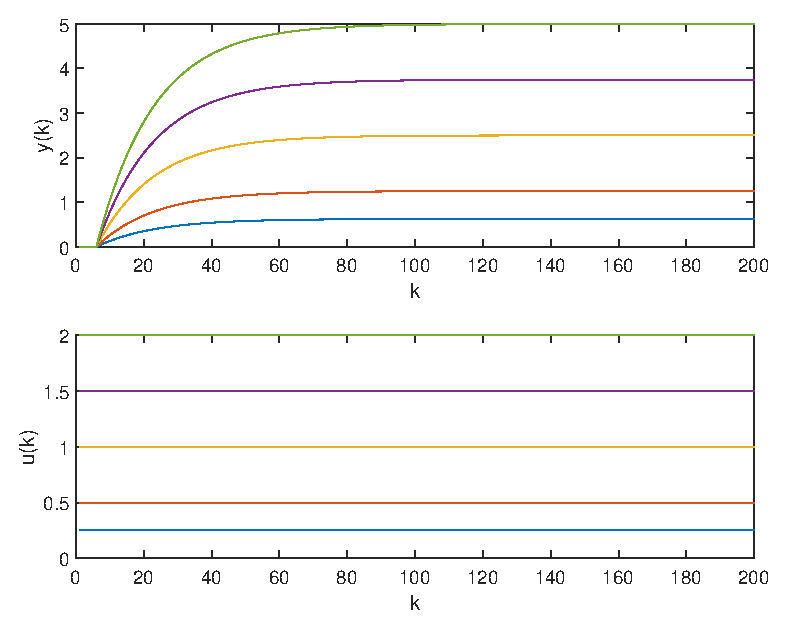
\includegraphics[scale=1]{Rys/odp_skok_u.eps}
    \caption{Odpowiedz procesu na skokową zmiane sterowania}
    \label{zad2_odp_skok_u}
\end{figure}

\begin{figure}[t]
	\centering
	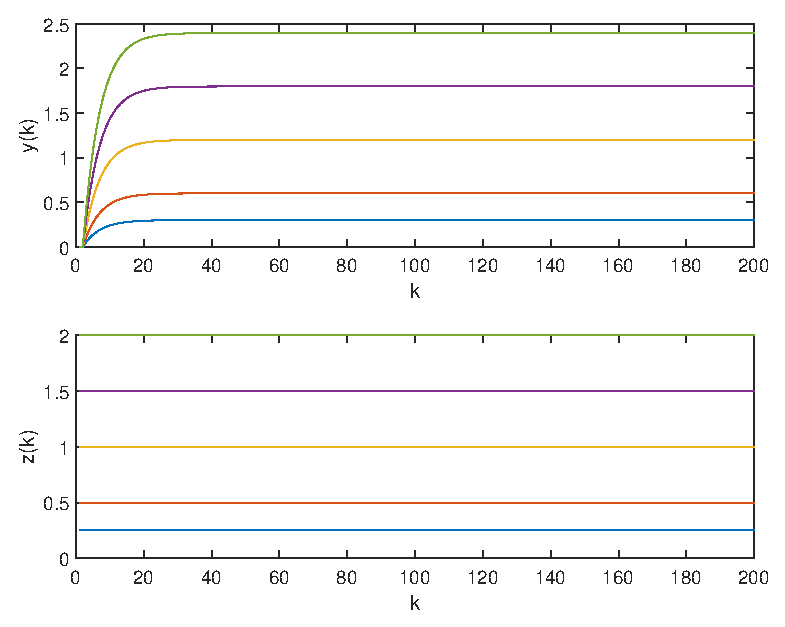
\includegraphics[scale=1]{Rys/odp_skok_z.eps}
	\caption{Odpowiedz procesu na skokową zmiane zakłócenia}
	\label{zad2_odp_skok_z}
\end{figure}

W celu wyznaczenia odpowiedzi skokowej obiekt, znajdujący się w punkcie pracy (tzn. $u= \num{0.0}$, $z= \num{0.0}$, $y= \num{0.0}$) pobudzony zostaje skokową wartością sterowania/zakłócenia. Rysunek \ref{zad2_odp_skok_u} oraz \ref{zad2_odp_skok_z} przedstawia odpowiedź obiektu na dane skoki.

\section{Wyznaczanie charakterystyki statycznej procesu}
\label{zad2_char_stat}
Aby wyznaczyć charakterystykę statyczną procesu przeprowadzono analogiczne działania co w rozdziale \ref{zad1}. Tym razem przy użyciu skryptu \verb+Zad2.m +dla wielu wartosci $u$ oraz $z$ wyznaczono odpowiadające im $y$ oraz z ich pomocą utworzono wykres \ref{zad2_char_stat}. Jak widać charakterystyka statyczna obiektu jest liniowa, a co za tym idzie obiekt jest liniowy.

\begin{figure}[b]   
     \label{zad2_char_stat}
    \centering
    % This file was created by matlab2tikz.
%
%The latest updates can be retrieved from
%  http://www.mathworks.com/matlabcentral/fileexchange/22022-matlab2tikz-matlab2tikz
%where you can also make suggestions and rate matlab2tikz.
%
\begin{tikzpicture}

\begin{axis}[%
width=3.56in,
height=3.566in,
at={(0.597in,0.481in)},
scale only axis,
xmin=0,
xmax=10,
tick align=outside,
xlabel style={font=\color{white!15!black}},
xlabel={z},
ymin=0,
ymax=10,
ylabel style={font=\color{white!15!black}},
ylabel={u},
zmin=0,
zmax=40,
zlabel style={font=\color{white!15!black}},
zlabel={y},
view={-37.5}{30},
axis background/.style={fill=white},
axis x line*=bottom,
axis y line*=left,
axis z line*=left,
xmajorgrids,
ymajorgrids,
zmajorgrids,
legend style={at={(1.03,1)}, anchor=north west, legend cell align=left, align=left, draw=white!15!black}
]

\addplot3[%
surf,
shader=flat corner, draw=black, z buffer=sort, colormap={mymap}{[1pt] rgb(0pt)=(0.2422,0.1504,0.6603); rgb(1pt)=(0.25039,0.164995,0.707614); rgb(2pt)=(0.257771,0.181781,0.751138); rgb(3pt)=(0.264729,0.197757,0.795214); rgb(4pt)=(0.270648,0.214676,0.836371); rgb(5pt)=(0.275114,0.234238,0.870986); rgb(6pt)=(0.2783,0.255871,0.899071); rgb(7pt)=(0.280333,0.278233,0.9221); rgb(8pt)=(0.281338,0.300595,0.941376); rgb(9pt)=(0.281014,0.322757,0.957886); rgb(10pt)=(0.279467,0.344671,0.971676); rgb(11pt)=(0.275971,0.366681,0.982905); rgb(12pt)=(0.269914,0.3892,0.9906); rgb(13pt)=(0.260243,0.412329,0.995157); rgb(14pt)=(0.244033,0.435833,0.998833); rgb(15pt)=(0.220643,0.460257,0.997286); rgb(16pt)=(0.196333,0.484719,0.989152); rgb(17pt)=(0.183405,0.507371,0.979795); rgb(18pt)=(0.178643,0.528857,0.968157); rgb(19pt)=(0.176438,0.549905,0.952019); rgb(20pt)=(0.168743,0.570262,0.935871); rgb(21pt)=(0.154,0.5902,0.9218); rgb(22pt)=(0.146029,0.609119,0.907857); rgb(23pt)=(0.138024,0.627629,0.89729); rgb(24pt)=(0.124814,0.645929,0.888343); rgb(25pt)=(0.111252,0.6635,0.876314); rgb(26pt)=(0.0952095,0.679829,0.859781); rgb(27pt)=(0.0688714,0.694771,0.839357); rgb(28pt)=(0.0296667,0.708167,0.816333); rgb(29pt)=(0.00357143,0.720267,0.7917); rgb(30pt)=(0.00665714,0.731214,0.766014); rgb(31pt)=(0.0433286,0.741095,0.73941); rgb(32pt)=(0.0963952,0.75,0.712038); rgb(33pt)=(0.140771,0.7584,0.684157); rgb(34pt)=(0.1717,0.766962,0.655443); rgb(35pt)=(0.193767,0.775767,0.6251); rgb(36pt)=(0.216086,0.7843,0.5923); rgb(37pt)=(0.246957,0.791795,0.556743); rgb(38pt)=(0.290614,0.79729,0.518829); rgb(39pt)=(0.340643,0.8008,0.478857); rgb(40pt)=(0.3909,0.802871,0.435448); rgb(41pt)=(0.445629,0.802419,0.390919); rgb(42pt)=(0.5044,0.7993,0.348); rgb(43pt)=(0.561562,0.794233,0.304481); rgb(44pt)=(0.617395,0.787619,0.261238); rgb(45pt)=(0.671986,0.779271,0.2227); rgb(46pt)=(0.7242,0.769843,0.191029); rgb(47pt)=(0.773833,0.759805,0.16461); rgb(48pt)=(0.820314,0.749814,0.153529); rgb(49pt)=(0.863433,0.7406,0.159633); rgb(50pt)=(0.903543,0.733029,0.177414); rgb(51pt)=(0.939257,0.728786,0.209957); rgb(52pt)=(0.972757,0.729771,0.239443); rgb(53pt)=(0.995648,0.743371,0.237148); rgb(54pt)=(0.996986,0.765857,0.219943); rgb(55pt)=(0.995205,0.789252,0.202762); rgb(56pt)=(0.9892,0.813567,0.188533); rgb(57pt)=(0.978629,0.838629,0.176557); rgb(58pt)=(0.967648,0.8639,0.16429); rgb(59pt)=(0.96101,0.889019,0.153676); rgb(60pt)=(0.959671,0.913457,0.142257); rgb(61pt)=(0.962795,0.937338,0.12651); rgb(62pt)=(0.969114,0.960629,0.106362); rgb(63pt)=(0.9769,0.9839,0.0805)}, mesh/rows=101]
table[row sep=crcr, point meta=\thisrow{c}] {%
%
x	y	z	c\\
0	0	0	0\\
0	0.1	0.249903474903477	0.249903474903477\\
0	0.2	0.499806949806954	0.499806949806954\\
0	0.3	0.749710424710437	0.749710424710437\\
0	0.4	0.999613899613908	0.999613899613908\\
0	0.5	1.2495173745174	1.2495173745174\\
0	0.6	1.49942084942087	1.49942084942087\\
0	0.7	1.74932432432434	1.74932432432434\\
0	0.8	1.99922779922782	1.99922779922782\\
0	0.9	2.24913127413129	2.24913127413129\\
0	1	2.4990347490348	2.4990347490348\\
0	1.1	2.74893822393823	2.74893822393823\\
0	1.2	2.99884169884175	2.99884169884175\\
0	1.3	3.24874517374517	3.24874517374517\\
0	1.4	3.49864864864869	3.49864864864869\\
0	1.5	3.74855212355212	3.74855212355212\\
0	1.6	3.99845559845563	3.99845559845563\\
0	1.7	4.24835907335906	4.24835907335906\\
0	1.8	4.49826254826259	4.49826254826259\\
0	1.9	4.74816602316607	4.74816602316607\\
0	2	4.99806949806959	4.99806949806959\\
0	2.1	5.24797297297295	5.24797297297295\\
0	2.2	5.49787644787646	5.49787644787646\\
0	2.3	5.74777992277997	5.74777992277997\\
0	2.4	5.9976833976835	5.9976833976835\\
0	2.5	6.24758687258684	6.24758687258684\\
0	2.6	6.49749034749034	6.49749034749034\\
0	2.7	6.74739382239386	6.74739382239386\\
0	2.8	6.99729729729738	6.99729729729738\\
0	2.9	7.24720077220089	7.24720077220089\\
0	3	7.49710424710424	7.49710424710424\\
0	3.1	7.74700772200776	7.74700772200776\\
0	3.2	7.99691119691127	7.99691119691127\\
0	3.3	8.2468146718148	8.2468146718148\\
0	3.4	8.49671814671812	8.49671814671812\\
0	3.5	8.74662162162165	8.74662162162165\\
0	3.6	8.99652509652518	8.99652509652518\\
0	3.7	9.24642857142863	9.24642857142863\\
0	3.8	9.49633204633214	9.49633204633214\\
0	3.9	9.74623552123566	9.74623552123566\\
0	4	9.99613899613918	9.99613899613918\\
0	4.1	10.2460424710424	10.2460424710424\\
0	4.2	10.4959459459459	10.4959459459459\\
0	4.3	10.7458494208494	10.7458494208494\\
0	4.4	10.9957528957529	10.9957528957529\\
0	4.5	11.2456563706564	11.2456563706564\\
0	4.6	11.4955598455599	11.4955598455599\\
0	4.7	11.7454633204635	11.7454633204635\\
0	4.8	11.995366795367	11.995366795367\\
0	4.9	12.2452702702705	12.2452702702705\\
0	5	12.4951737451737	12.4951737451737\\
0	5.1	12.7450772200772	12.7450772200772\\
0	5.2	12.9949806949807	12.9949806949807\\
0	5.3	13.2448841698842	13.2448841698842\\
0	5.4	13.4947876447877	13.4947876447877\\
0	5.5	13.7446911196912	13.7446911196912\\
0	5.6	13.9945945945948	13.9945945945948\\
0	5.7	14.2444980694983	14.2444980694983\\
0	5.8	14.4944015444018	14.4944015444018\\
0	5.9	14.744305019305	14.744305019305\\
0	6	14.9942084942085	14.9942084942085\\
0	6.1	15.244111969112	15.244111969112\\
0	6.2	15.4940154440155	15.4940154440155\\
0	6.3	15.743918918919	15.743918918919\\
0	6.4	15.9938223938225	15.9938223938225\\
0	6.5	16.2437258687261	16.2437258687261\\
0	6.6	16.4936293436296	16.4936293436296\\
0	6.7	16.7435328185328	16.7435328185328\\
0	6.8	16.9934362934362	16.9934362934362\\
0	6.9	17.2433397683398	17.2433397683398\\
0	7	17.4932432432433	17.4932432432433\\
0	7.1	17.7431467181468	17.7431467181468\\
0	7.2	17.9930501930504	17.9930501930504\\
0	7.3	18.2429536679538	18.2429536679538\\
0	7.4	18.4928571428573	18.4928571428573\\
0	7.5	18.7427606177608	18.7427606177608\\
0	7.6	18.9926640926643	18.9926640926643\\
0	7.7	19.2425675675679	19.2425675675679\\
0	7.8	19.4924710424713	19.4924710424713\\
0	7.9	19.7423745173749	19.7423745173749\\
0	8	19.9922779922784	19.9922779922784\\
0	8.1	20.2421814671812	20.2421814671812\\
0	8.2	20.4920849420847	20.4920849420847\\
0	8.3	20.7419884169883	20.7419884169883\\
0	8.4	20.9918918918918	20.9918918918918\\
0	8.5	21.2417953667953	21.2417953667953\\
0	8.6	21.4916988416988	21.4916988416988\\
0	8.7	21.7416023166023	21.7416023166023\\
0	8.8	21.9915057915059	21.9915057915059\\
0	8.9	22.2414092664094	22.2414092664094\\
0	9	22.4913127413129	22.4913127413129\\
0	9.1	22.7412162162164	22.7412162162164\\
0	9.2	22.9911196911199	22.9911196911199\\
0	9.3	23.2410231660234	23.2410231660234\\
0	9.4	23.4909266409269	23.4909266409269\\
0	9.5	23.7408301158305	23.7408301158305\\
0	9.6	23.990733590734	23.990733590734\\
0	9.7	24.2406370656375	24.2406370656375\\
0	9.8	24.490540540541	24.490540540541\\
0	9.9	24.7404440154438	24.7404440154438\\
0	10	24.9903474903474	24.9903474903474\\
0.1	0	0.11988416988417	0.11988416988417\\
0.1	0.1	0.369787644787649	0.369787644787649\\
0.1	0.2	0.61969111969113	0.61969111969113\\
0.1	0.3	0.869594594594604	0.869594594594604\\
0.1	0.4	1.11949806949808	1.11949806949808\\
0.1	0.5	1.36940154440157	1.36940154440157\\
0.1	0.6	1.61930501930504	1.61930501930504\\
0.1	0.7	1.86920849420851	1.86920849420851\\
0.1	0.8	2.11911196911198	2.11911196911198\\
0.1	0.9	2.36901544401549	2.36901544401549\\
0.1	1	2.61891891891893	2.61891891891893\\
0.1	1.1	2.86882239382244	2.86882239382244\\
0.1	1.2	3.11872586872586	3.11872586872586\\
0.1	1.3	3.36862934362938	3.36862934362938\\
0.1	1.4	3.61853281853282	3.61853281853282\\
0.1	1.5	3.86843629343633	3.86843629343633\\
0.1	1.6	4.11833976833977	4.11833976833977\\
0.1	1.7	4.36824324324329	4.36824324324329\\
0.1	1.8	4.61814671814668	4.61814671814668\\
0.1	1.9	4.86805019305021	4.86805019305021\\
0.1	2	5.11795366795373	5.11795366795373\\
0.1	2.1	5.36785714285725	5.36785714285725\\
0.1	2.2	5.61776061776058	5.61776061776058\\
0.1	2.3	5.8676640926641	5.8676640926641\\
0.1	2.4	6.11756756756761	6.11756756756761\\
0.1	2.5	6.36747104247113	6.36747104247113\\
0.1	2.6	6.61737451737448	6.61737451737448\\
0.1	2.7	6.86727799227799	6.86727799227799\\
0.1	2.8	7.1171814671815	7.1171814671815\\
0.1	2.9	7.36708494208501	7.36708494208501\\
0.1	3	7.61698841698853	7.61698841698853\\
0.1	3.1	7.86689189189188	7.86689189189188\\
0.1	3.2	8.11679536679543	8.11679536679543\\
0.1	3.3	8.36669884169891	8.36669884169891\\
0.1	3.4	8.6166023166024	8.6166023166024\\
0.1	3.5	8.86650579150579	8.86650579150579\\
0.1	3.6	9.11640926640946	9.11640926640946\\
0.1	3.7	9.36631274131295	9.36631274131295\\
0.1	3.8	9.6162162162161	9.6162162162161\\
0.1	3.9	9.86611969111962	9.86611969111962\\
0.1	4	10.1160231660232	10.1160231660232\\
0.1	4.1	10.3659266409267	10.3659266409267\\
0.1	4.2	10.6158301158302	10.6158301158302\\
0.1	4.3	10.8657335907337	10.8657335907337\\
0.1	4.4	11.1156370656372	11.1156370656372\\
0.1	4.5	11.3655405405407	11.3655405405407\\
0.1	4.6	11.6154440154442	11.6154440154442\\
0.1	4.7	11.8653474903474	11.8653474903474\\
0.1	4.8	12.1152509652509	12.1152509652509\\
0.1	4.9	12.3651544401544	12.3651544401544\\
0.1	5	12.6150579150579	12.6150579150579\\
0.1	5.1	12.8649613899615	12.8649613899615\\
0.1	5.2	13.114864864865	13.114864864865\\
0.1	5.3	13.3647683397685	13.3647683397685\\
0.1	5.4	13.614671814672	13.614671814672\\
0.1	5.5	13.8645752895755	13.8645752895755\\
0.1	5.6	14.1144787644787	14.1144787644787\\
0.1	5.7	14.3643822393822	14.3643822393822\\
0.1	5.8	14.6142857142857	14.6142857142857\\
0.1	5.9	14.8641891891893	14.8641891891893\\
0.1	6	15.1140926640928	15.1140926640928\\
0.1	6.1	15.3639961389963	15.3639961389963\\
0.1	6.2	15.6138996138998	15.6138996138998\\
0.1	6.3	15.8638030888033	15.8638030888033\\
0.1	6.4	16.1137065637065	16.1137065637065\\
0.1	6.5	16.36361003861	16.36361003861\\
0.1	6.6	16.6135135135136	16.6135135135136\\
0.1	6.7	16.8634169884171	16.8634169884171\\
0.1	6.8	17.1133204633206	17.1133204633206\\
0.1	6.9	17.3632239382241	17.3632239382241\\
0.1	7	17.6131274131275	17.6131274131275\\
0.1	7.1	17.8630308880312	17.8630308880312\\
0.1	7.2	18.1129343629344	18.1129343629344\\
0.1	7.3	18.3628378378377	18.3628378378377\\
0.1	7.4	18.6127413127413	18.6127413127413\\
0.1	7.5	18.8626447876447	18.8626447876447\\
0.1	7.6	19.1125482625483	19.1125482625483\\
0.1	7.7	19.3624517374518	19.3624517374518\\
0.1	7.8	19.6123552123553	19.6123552123553\\
0.1	7.9	19.8622586872588	19.8622586872588\\
0.1	8	20.1121621621623	20.1121621621623\\
0.1	8.1	20.3620656370659	20.3620656370659\\
0.1	8.2	20.6119691119694	20.6119691119694\\
0.1	8.3	20.8618725868729	20.8618725868729\\
0.1	8.4	21.1117760617764	21.1117760617764\\
0.1	8.5	21.36167953668	21.36167953668\\
0.1	8.6	21.6115830115834	21.6115830115834\\
0.1	8.7	21.8614864864862	21.8614864864862\\
0.1	8.8	22.1113899613898	22.1113899613898\\
0.1	8.9	22.3612934362933	22.3612934362933\\
0.1	9	22.6111969111968	22.6111969111968\\
0.1	9.1	22.8611003861003	22.8611003861003\\
0.1	9.2	23.1110038610038	23.1110038610038\\
0.1	9.3	23.3609073359074	23.3609073359074\\
0.1	9.4	23.6108108108109	23.6108108108109\\
0.1	9.5	23.8607142857144	23.8607142857144\\
0.1	9.6	24.1106177606179	24.1106177606179\\
0.1	9.7	24.3605212355214	24.3605212355214\\
0.1	9.8	24.6104247104249	24.6104247104249\\
0.1	9.9	24.8603281853285	24.8603281853285\\
0.1	10	25.110231660232	25.110231660232\\
0.2	0	0.23976833976834	0.23976833976834\\
0.2	0.1	0.489671814671816	0.489671814671816\\
0.2	0.2	0.739575289575299	0.739575289575299\\
0.2	0.3	0.989478764478772	0.989478764478772\\
0.2	0.4	1.23938223938226	1.23938223938226\\
0.2	0.5	1.48928571428573	1.48928571428573\\
0.2	0.6	1.73918918918921	1.73918918918921\\
0.2	0.7	1.98909266409268	1.98909266409268\\
0.2	0.8	2.23899613899616	2.23899613899616\\
0.2	0.9	2.48889961389962	2.48889961389962\\
0.2	1	2.73880308880314	2.73880308880314\\
0.2	1.1	2.98870656370656	2.98870656370656\\
0.2	1.2	3.23861003861008	3.23861003861008\\
0.2	1.3	3.48851351351351	3.48851351351351\\
0.2	1.4	3.73841698841702	3.73841698841702\\
0.2	1.5	3.98832046332045	3.98832046332045\\
0.2	1.6	4.23822393822397	4.23822393822397\\
0.2	1.7	4.4881274131274	4.4881274131274\\
0.2	1.8	4.73803088803099	4.73803088803099\\
0.2	1.9	4.98793436293433	4.98793436293433\\
0.2	2	5.23783783783785	5.23783783783785\\
0.2	2.1	5.48774131274137	5.48774131274137\\
0.2	2.2	5.73764478764488	5.73764478764488\\
0.2	2.3	5.98754826254822	5.98754826254822\\
0.2	2.4	6.23745173745173	6.23745173745173\\
0.2	2.5	6.48735521235526	6.48735521235526\\
0.2	2.6	6.73725868725877	6.73725868725877\\
0.2	2.7	6.98716216216228	6.98716216216228\\
0.2	2.8	7.23706563706563	7.23706563706563\\
0.2	2.9	7.48696911196915	7.48696911196915\\
0.2	3	7.73687258687266	7.73687258687266\\
0.2	3.1	7.98677606177617	7.98677606177617\\
0.2	3.2	8.23667953667953	8.23667953667953\\
0.2	3.3	8.48658301158305	8.48658301158305\\
0.2	3.4	8.73648648648658	8.73648648648658\\
0.2	3.5	8.9863899613901	8.9863899613901\\
0.2	3.6	9.23629343629335	9.23629343629335\\
0.2	3.7	9.48619691119689	9.48619691119689\\
0.2	3.8	9.73610038610041	9.73610038610041\\
0.2	3.9	9.98600386100393	9.98600386100393\\
0.2	4	10.2359073359075	10.2359073359075\\
0.2	4.1	10.485810810811	10.485810810811\\
0.2	4.2	10.7357142857145	10.7357142857145\\
0.2	4.3	10.9856177606176	10.9856177606176\\
0.2	4.4	11.2355212355212	11.2355212355212\\
0.2	4.5	11.4854247104247	11.4854247104247\\
0.2	4.6	11.7353281853282	11.7353281853282\\
0.2	4.7	11.9852316602317	11.9852316602317\\
0.2	4.8	12.2351351351352	12.2351351351352\\
0.2	4.9	12.4850386100387	12.4850386100387\\
0.2	5	12.7349420849423	12.7349420849423\\
0.2	5.1	12.9848455598458	12.9848455598458\\
0.2	5.2	13.234749034749	13.234749034749\\
0.2	5.3	13.4846525096525	13.4846525096525\\
0.2	5.4	13.734555984556	13.734555984556\\
0.2	5.5	13.9844594594595	13.9844594594595\\
0.2	5.6	14.234362934363	14.234362934363\\
0.2	5.7	14.4842664092665	14.4842664092665\\
0.2	5.8	14.73416988417	14.73416988417\\
0.2	5.9	14.9840733590736	14.9840733590736\\
0.2	6	15.2339768339771	15.2339768339771\\
0.2	6.1	15.4838803088802	15.4838803088802\\
0.2	6.2	15.7337837837838	15.7337837837838\\
0.2	6.3	15.9836872586873	15.9836872586873\\
0.2	6.4	16.2335907335909	16.2335907335909\\
0.2	6.5	16.4834942084943	16.4834942084943\\
0.2	6.6	16.7333976833978	16.7333976833978\\
0.2	6.7	16.9833011583014	16.9833011583014\\
0.2	6.8	17.2332046332048	17.2332046332048\\
0.2	6.9	17.4831081081084	17.4831081081084\\
0.2	7	17.7330115830116	17.7330115830116\\
0.2	7.1	17.9829150579151	17.9829150579151\\
0.2	7.2	18.2328185328189	18.2328185328189\\
0.2	7.3	18.4827220077224	18.4827220077224\\
0.2	7.4	18.7326254826259	18.7326254826259\\
0.2	7.5	18.9825289575287	18.9825289575287\\
0.2	7.6	19.2324324324322	19.2324324324322\\
0.2	7.7	19.4823359073357	19.4823359073357\\
0.2	7.8	19.7322393822392	19.7322393822392\\
0.2	7.9	19.9821428571428	19.9821428571428\\
0.2	8	20.2320463320463	20.2320463320463\\
0.2	8.1	20.4819498069498	20.4819498069498\\
0.2	8.2	20.7318532818534	20.7318532818534\\
0.2	8.3	20.9817567567569	20.9817567567569\\
0.2	8.4	21.2316602316604	21.2316602316604\\
0.2	8.5	21.4815637065639	21.4815637065639\\
0.2	8.6	21.7314671814674	21.7314671814674\\
0.2	8.7	21.9813706563709	21.9813706563709\\
0.2	8.8	22.2312741312745	22.2312741312745\\
0.2	8.9	22.4811776061779	22.4811776061779\\
0.2	9	22.7310810810815	22.7310810810815\\
0.2	9.1	22.980984555985	22.980984555985\\
0.2	9.2	23.2308880308885	23.2308880308885\\
0.2	9.3	23.4807915057913	23.4807915057913\\
0.2	9.4	23.7306949806949	23.7306949806949\\
0.2	9.5	23.9805984555983	23.9805984555983\\
0.2	9.6	24.2305019305018	24.2305019305018\\
0.2	9.7	24.4804054054054	24.4804054054054\\
0.2	9.8	24.7303088803089	24.7303088803089\\
0.2	9.9	24.9802123552124	24.9802123552124\\
0.2	10	25.2301158301159	25.2301158301159\\
0.3	0	0.359652509652514	0.359652509652514\\
0.3	0.1	0.609555984555993	0.609555984555993\\
0.3	0.2	0.859459459459466	0.859459459459466\\
0.3	0.3	1.10936293436294	1.10936293436294\\
0.3	0.4	1.35926640926643	1.35926640926643\\
0.3	0.5	1.6091698841699	1.6091698841699\\
0.3	0.6	1.85907335907337	1.85907335907337\\
0.3	0.7	2.10897683397685	2.10897683397685\\
0.3	0.8	2.35888030888032	2.35888030888032\\
0.3	0.9	2.60878378378383	2.60878378378383\\
0.3	1	2.85868725868726	2.85868725868726\\
0.3	1.1	3.10859073359078	3.10859073359078\\
0.3	1.2	3.3584942084942	3.3584942084942\\
0.3	1.3	3.60839768339772	3.60839768339772\\
0.3	1.4	3.85830115830115	3.85830115830115\\
0.3	1.5	4.10820463320466	4.10820463320466\\
0.3	1.6	4.35810810810809	4.35810810810809\\
0.3	1.7	4.60801158301158	4.60801158301158\\
0.3	1.8	4.85791505791511	4.85791505791511\\
0.3	1.9	5.10781853281862	5.10781853281862\\
0.3	2	5.35772200772198	5.35772200772198\\
0.3	2.1	5.60762548262549	5.60762548262549\\
0.3	2.2	5.857528957529	5.857528957529\\
0.3	2.3	6.10743243243253	6.10743243243253\\
0.3	2.4	6.35733590733587	6.35733590733587\\
0.3	2.5	6.60723938223936	6.60723938223936\\
0.3	2.6	6.85714285714289	6.85714285714289\\
0.3	2.7	7.10704633204641	7.10704633204641\\
0.3	2.8	7.35694980694992	7.35694980694992\\
0.3	2.9	7.60685328185327	7.60685328185327\\
0.3	3	7.85675675675679	7.85675675675679\\
0.3	3.1	8.10666023166028	8.10666023166028\\
0.3	3.2	8.35656370656383	8.35656370656383\\
0.3	3.3	8.60646718146715	8.60646718146715\\
0.3	3.4	8.85637065637068	8.85637065637068\\
0.3	3.5	9.10627413127414	9.10627413127414\\
0.3	3.6	9.35617760617766	9.35617760617766\\
0.3	3.7	9.6060810810812	9.6060810810812\\
0.3	3.8	9.85598455598469	9.85598455598469\\
0.3	3.9	10.1058880308882	10.1058880308882\\
0.3	4	10.3557915057914	10.3557915057914\\
0.3	4.1	10.6056949806949	10.6056949806949\\
0.3	4.2	10.8555984555984	10.8555984555984\\
0.3	4.3	11.105501930502	11.105501930502\\
0.3	4.4	11.3554054054055	11.3554054054055\\
0.3	4.5	11.605308880309	11.605308880309\\
0.3	4.6	11.8552123552125	11.8552123552125\\
0.3	4.7	12.105115830116	12.105115830116\\
0.3	4.8	12.3550193050195	12.3550193050195\\
0.3	4.9	12.6049227799227	12.6049227799227\\
0.3	5	12.8548262548262	12.8548262548262\\
0.3	5.1	13.1047297297297	13.1047297297297\\
0.3	5.2	13.3546332046332	13.3546332046332\\
0.3	5.3	13.6045366795368	13.6045366795368\\
0.3	5.4	13.8544401544403	13.8544401544403\\
0.3	5.5	14.1043436293438	14.1043436293438\\
0.3	5.6	14.3542471042473	14.3542471042473\\
0.3	5.7	14.6041505791508	14.6041505791508\\
0.3	5.8	14.854054054054	14.854054054054\\
0.3	5.9	15.1039575289575	15.1039575289575\\
0.3	6	15.353861003861	15.353861003861\\
0.3	6.1	15.6037644787645	15.6037644787645\\
0.3	6.2	15.853667953668	15.853667953668\\
0.3	6.3	16.1035714285715	16.1035714285715\\
0.3	6.4	16.3534749034752	16.3534749034752\\
0.3	6.5	16.6033783783786	16.6033783783786\\
0.3	6.6	16.8532818532821	16.8532818532821\\
0.3	6.7	17.1031853281853	17.1031853281853\\
0.3	6.8	17.3530888030888	17.3530888030888\\
0.3	6.9	17.6029922779923	17.6029922779923\\
0.3	7	17.8528957528958	17.8528957528958\\
0.3	7.1	18.1027992277994	18.1027992277994\\
0.3	7.2	18.3527027027028	18.3527027027028\\
0.3	7.3	18.6026061776063	18.6026061776063\\
0.3	7.4	18.8525096525099	18.8525096525099\\
0.3	7.5	19.1024131274133	19.1024131274133\\
0.3	7.6	19.3523166023169	19.3523166023169\\
0.3	7.7	19.6022200772203	19.6022200772203\\
0.3	7.8	19.8521235521239	19.8521235521239\\
0.3	7.9	20.1020270270274	20.1020270270274\\
0.3	8	20.3519305019302	20.3519305019302\\
0.3	8.1	20.6018339768338	20.6018339768338\\
0.3	8.2	20.8517374517373	20.8517374517373\\
0.3	8.3	21.1016409266408	21.1016409266408\\
0.3	8.4	21.3515444015443	21.3515444015443\\
0.3	8.5	21.6014478764478	21.6014478764478\\
0.3	8.6	21.8513513513513	21.8513513513513\\
0.3	8.7	22.1012548262549	22.1012548262549\\
0.3	8.8	22.3511583011584	22.3511583011584\\
0.3	8.9	22.6010617760619	22.6010617760619\\
0.3	9	22.8509652509654	22.8509652509654\\
0.3	9.1	23.1008687258689	23.1008687258689\\
0.3	9.2	23.3507722007724	23.3507722007724\\
0.3	9.3	23.600675675676	23.600675675676\\
0.3	9.4	23.8505791505795	23.8505791505795\\
0.3	9.5	24.100482625483	24.100482625483\\
0.3	9.6	24.3503861003865	24.3503861003865\\
0.3	9.7	24.60028957529	24.60028957529\\
0.3	9.8	24.8501930501929	24.8501930501929\\
0.3	9.9	25.1000965250963	25.1000965250963\\
0.3	10	25.3499999999999	25.3499999999999\\
0.4	0	0.47953667953668	0.47953667953668\\
0.4	0.1	0.729440154440162	0.729440154440162\\
0.4	0.2	0.979343629343632	0.979343629343632\\
0.4	0.3	1.22924710424712	1.22924710424712\\
0.4	0.4	1.4791505791506	1.4791505791506\\
0.4	0.5	1.72905405405407	1.72905405405407\\
0.4	0.6	1.97895752895754	1.97895752895754\\
0.4	0.7	2.22886100386102	2.22886100386102\\
0.4	0.8	2.47876447876452	2.47876447876452\\
0.4	0.9	2.72866795366796	2.72866795366796\\
0.4	1	2.97857142857147	2.97857142857147\\
0.4	1.1	3.22847490347489	3.22847490347489\\
0.4	1.2	3.47837837837842	3.47837837837842\\
0.4	1.3	3.72828185328185	3.72828185328185\\
0.4	1.4	3.97818532818536	3.97818532818536\\
0.4	1.5	4.2280888030888	4.2280888030888\\
0.4	1.6	4.47799227799232	4.47799227799232\\
0.4	1.7	4.72789575289572	4.72789575289572\\
0.4	1.8	4.97779922779923	4.97779922779923\\
0.4	1.9	5.22770270270276	5.22770270270276\\
0.4	2	5.47760617760627	5.47760617760627\\
0.4	2.1	5.72750965250961	5.72750965250961\\
0.4	2.2	5.97741312741313	5.97741312741313\\
0.4	2.3	6.22731660231664	6.22731660231664\\
0.4	2.4	6.47722007722016	6.47722007722016\\
0.4	2.5	6.7271235521235	6.7271235521235\\
0.4	2.6	6.97702702702702	6.97702702702702\\
0.4	2.7	7.22693050193054	7.22693050193054\\
0.4	2.8	7.47683397683404	7.47683397683404\\
0.4	2.9	7.72673745173757	7.72673745173757\\
0.4	3	7.97664092664091	7.97664092664091\\
0.4	3.1	8.22654440154446	8.22654440154446\\
0.4	3.2	8.47644787644794	8.47644787644794\\
0.4	3.3	8.72635135135146	8.72635135135146\\
0.4	3.4	8.97625482625479	8.97625482625479\\
0.4	3.5	9.22615830115849	9.22615830115849\\
0.4	3.6	9.47606177606198	9.47606177606198\\
0.4	3.7	9.72596525096513	9.72596525096513\\
0.4	3.8	9.97586872586865	9.97586872586865\\
0.4	3.9	10.2257722007722	10.2257722007722\\
0.4	4	10.4756756756757	10.4756756756757\\
0.4	4.1	10.7255791505792	10.7255791505792\\
0.4	4.2	10.9754826254827	10.9754826254827\\
0.4	4.3	11.2253861003863	11.2253861003863\\
0.4	4.4	11.4752895752898	11.4752895752898\\
0.4	4.5	11.7251930501933	11.7251930501933\\
0.4	4.6	11.9750965250964	11.9750965250964\\
0.4	4.7	12.225	12.225\\
0.4	4.8	12.4749034749035	12.4749034749035\\
0.4	4.9	12.724806949807	12.724806949807\\
0.4	5	12.9747104247105	12.9747104247105\\
0.4	5.1	13.224613899614	13.224613899614\\
0.4	5.2	13.4745173745175	13.4745173745175\\
0.4	5.3	13.7244208494211	13.7244208494211\\
0.4	5.4	13.9743243243246	13.9743243243246\\
0.4	5.5	14.2242277992277	14.2242277992277\\
0.4	5.6	14.4741312741313	14.4741312741313\\
0.4	5.7	14.7240347490348	14.7240347490348\\
0.4	5.8	14.9739382239383	14.9739382239383\\
0.4	5.9	15.2238416988418	15.2238416988418\\
0.4	6	15.4737451737453	15.4737451737453\\
0.4	6.1	15.7236486486488	15.7236486486488\\
0.4	6.2	15.9735521235523	15.9735521235523\\
0.4	6.3	16.2234555984555	16.2234555984555\\
0.4	6.4	16.4733590733591	16.4733590733591\\
0.4	6.5	16.7232625482626	16.7232625482626\\
0.4	6.6	16.9731660231661	16.9731660231661\\
0.4	6.7	17.2230694980696	17.2230694980696\\
0.4	6.8	17.4729729729732	17.4729729729732\\
0.4	6.9	17.7228764478766	17.7228764478766\\
0.4	7	17.9727799227802	17.9727799227802\\
0.4	7.1	18.2226833976832	18.2226833976832\\
0.4	7.2	18.4725868725867	18.4725868725867\\
0.4	7.3	18.7224903474903	18.7224903474903\\
0.4	7.4	18.9723938223938	18.9723938223938\\
0.4	7.5	19.2222972972973	19.2222972972973\\
0.4	7.6	19.4722007722008	19.4722007722008\\
0.4	7.7	19.7221042471043	19.7221042471043\\
0.4	7.8	19.9720077220079	19.9720077220079\\
0.4	7.9	20.2219111969114	20.2219111969114\\
0.4	8	20.4718146718149	20.4718146718149\\
0.4	8.1	20.7217181467184	20.7217181467184\\
0.4	8.2	20.971621621622	20.971621621622\\
0.4	8.3	21.2215250965254	21.2215250965254\\
0.4	8.4	21.471428571429	21.471428571429\\
0.4	8.5	21.7213320463325	21.7213320463325\\
0.4	8.6	21.9712355212353	21.9712355212353\\
0.4	8.7	22.2211389961388	22.2211389961388\\
0.4	8.8	22.4710424710423	22.4710424710423\\
0.4	8.9	22.7209459459459	22.7209459459459\\
0.4	9	22.9708494208493	22.9708494208493\\
0.4	9.1	23.2207528957528	23.2207528957528\\
0.4	9.2	23.4706563706564	23.4706563706564\\
0.4	9.3	23.7205598455599	23.7205598455599\\
0.4	9.4	23.9704633204634	23.9704633204634\\
0.4	9.5	24.220366795367	24.220366795367\\
0.4	9.6	24.4702702702704	24.4702702702704\\
0.4	9.7	24.720173745174	24.720173745174\\
0.4	9.8	24.9700772200775	24.9700772200775\\
0.4	9.9	25.219980694981	25.219980694981\\
0.4	10	25.4698841698845	25.4698841698845\\
0.5	0	0.59942084942086	0.59942084942086\\
0.5	0.1	0.849324324324329	0.849324324324329\\
0.5	0.2	1.09922779922781	1.09922779922781\\
0.5	0.3	1.34913127413129	1.34913127413129\\
0.5	0.4	1.59903474903477	1.59903474903477\\
0.5	0.5	1.84893822393824	1.84893822393824\\
0.5	0.6	2.09884169884171	2.09884169884171\\
0.5	0.7	2.34874517374522	2.34874517374522\\
0.5	0.8	2.59864864864865	2.59864864864865\\
0.5	0.9	2.84855212355217	2.84855212355217\\
0.5	1	3.09845559845559	3.09845559845559\\
0.5	1.1	3.34835907335911	3.34835907335911\\
0.5	1.2	3.59826254826254	3.59826254826254\\
0.5	1.3	3.84816602316605	3.84816602316605\\
0.5	1.4	4.0980694980695	4.0980694980695\\
0.5	1.5	4.34797297297302	4.34797297297302\\
0.5	1.6	4.59787644787651	4.59787644787651\\
0.5	1.7	4.84777992278001	4.84777992278001\\
0.5	1.8	5.09768339768336	5.09768339768336\\
0.5	1.9	5.34758687258688	5.34758687258688\\
0.5	2	5.59749034749039	5.59749034749039\\
0.5	2.1	5.84739382239391	5.84739382239391\\
0.5	2.2	6.09729729729726	6.09729729729726\\
0.5	2.3	6.34720077220076	6.34720077220076\\
0.5	2.4	6.59710424710429	6.59710424710429\\
0.5	2.5	6.8470077220078	6.8470077220078\\
0.5	2.6	7.09691119691131	7.09691119691131\\
0.5	2.7	7.34681467181466	7.34681467181466\\
0.5	2.8	7.59671814671818	7.59671814671818\\
0.5	2.9	7.84662162162169	7.84662162162169\\
0.5	3	8.09652509652524	8.09652509652524\\
0.5	3.1	8.34642857142856	8.34642857142856\\
0.5	3.2	8.59633204633208	8.59633204633208\\
0.5	3.3	8.84623552123561	8.84623552123561\\
0.5	3.4	9.09613899613889	9.09613899613889\\
0.5	3.5	9.34604247104241	9.34604247104241\\
0.5	3.6	9.59594594594592	9.59594594594592\\
0.5	3.7	9.84584942084944	9.84584942084944\\
0.5	3.8	10.0957528957529	10.0957528957529\\
0.5	3.9	10.3456563706565	10.3456563706565\\
0.5	4	10.59555984556	10.59555984556\\
0.5	4.1	10.8454633204635	10.8454633204635\\
0.5	4.2	11.0953667953667	11.0953667953667\\
0.5	4.3	11.3452702702702	11.3452702702702\\
0.5	4.4	11.5951737451737	11.5951737451737\\
0.5	4.5	11.8450772200772	11.8450772200772\\
0.5	4.6	12.0949806949807	12.0949806949807\\
0.5	4.7	12.3448841698842	12.3448841698842\\
0.5	4.8	12.5947876447878	12.5947876447878\\
0.5	4.9	12.8446911196913	12.8446911196913\\
0.5	5	13.0945945945948	13.0945945945948\\
0.5	5.1	13.344498069498	13.344498069498\\
0.5	5.2	13.5944015444015	13.5944015444015\\
0.5	5.3	13.844305019305	13.844305019305\\
0.5	5.4	14.0942084942085	14.0942084942085\\
0.5	5.5	14.3441119691121	14.3441119691121\\
0.5	5.6	14.5940154440155	14.5940154440155\\
0.5	5.7	14.843918918919	14.843918918919\\
0.5	5.8	15.0938223938226	15.0938223938226\\
0.5	5.9	15.3437258687261	15.3437258687261\\
0.5	6	15.5936293436293	15.5936293436293\\
0.5	6.1	15.8435328185328	15.8435328185328\\
0.5	6.2	16.0934362934363	16.0934362934363\\
0.5	6.3	16.3433397683399	16.3433397683399\\
0.5	6.4	16.5932432432434	16.5932432432434\\
0.5	6.5	16.8431467181468	16.8431467181468\\
0.5	6.6	17.0930501930504	17.0930501930504\\
0.5	6.7	17.3429536679539	17.3429536679539\\
0.5	6.8	17.5928571428575	17.5928571428575\\
0.5	6.9	17.8427606177606	17.8427606177606\\
0.5	7	18.0926640926642	18.0926640926642\\
0.5	7.1	18.342567567568	18.342567567568\\
0.5	7.2	18.5924710424714	18.5924710424714\\
0.5	7.3	18.8423745173742	18.8423745173742\\
0.5	7.4	19.0922779922778	19.0922779922778\\
0.5	7.5	19.3421814671812	19.3421814671812\\
0.5	7.6	19.5920849420847	19.5920849420847\\
0.5	7.7	19.8419884169883	19.8419884169883\\
0.5	7.8	20.0918918918917	20.0918918918917\\
0.5	7.9	20.3417953667953	20.3417953667953\\
0.5	8	20.5916988416988	20.5916988416988\\
0.5	8.1	20.8416023166024	20.8416023166024\\
0.5	8.2	21.0915057915059	21.0915057915059\\
0.5	8.3	21.3414092664094	21.3414092664094\\
0.5	8.4	21.5913127413129	21.5913127413129\\
0.5	8.5	21.8412162162164	21.8412162162164\\
0.5	8.6	22.09111969112	22.09111969112\\
0.5	8.7	22.3410231660235	22.3410231660235\\
0.5	8.8	22.590926640927	22.590926640927\\
0.5	8.9	22.8408301158305	22.8408301158305\\
0.5	9	23.090733590734	23.090733590734\\
0.5	9.1	23.3406370656369	23.3406370656369\\
0.5	9.2	23.5905405405403	23.5905405405403\\
0.5	9.3	23.8404440154439	23.8404440154439\\
0.5	9.4	24.0903474903474	24.0903474903474\\
0.5	9.5	24.3402509652509	24.3402509652509\\
0.5	9.6	24.5901544401544	24.5901544401544\\
0.5	9.7	24.8400579150579	24.8400579150579\\
0.5	9.8	25.0899613899614	25.0899613899614\\
0.5	9.9	25.3398648648649	25.3398648648649\\
0.5	10	25.5897683397685	25.5897683397685\\
0.6	0	0.719305019305027	0.719305019305027\\
0.6	0.1	0.969208494208496	0.969208494208496\\
0.6	0.2	1.21911196911199	1.21911196911199\\
0.6	0.3	1.46901544401546	1.46901544401546\\
0.6	0.4	1.71891891891893	1.71891891891893\\
0.6	0.5	1.9688223938224	1.9688223938224\\
0.6	0.6	2.21872586872588	2.21872586872588\\
0.6	0.7	2.46862934362934	2.46862934362934\\
0.6	0.8	2.71853281853286	2.71853281853286\\
0.6	0.9	2.96843629343629	2.96843629343629\\
0.6	1	3.21833976833981	3.21833976833981\\
0.6	1.1	3.46824324324324	3.46824324324324\\
0.6	1.2	3.71814671814675	3.71814671814675\\
0.6	1.3	3.96805019305018	3.96805019305018\\
0.6	1.4	4.2179536679537	4.2179536679537\\
0.6	1.5	4.46785714285721	4.46785714285721\\
0.6	1.6	4.71776061776064	4.71776061776064\\
0.6	1.7	4.96766409266414	4.96766409266414\\
0.6	1.8	5.21756756756766	5.21756756756766\\
0.6	1.9	5.467471042471	5.467471042471\\
0.6	2	5.71737451737452	5.71737451737452\\
0.6	2.1	5.96727799227803	5.96727799227803\\
0.6	2.2	6.21718146718156	6.21718146718156\\
0.6	2.3	6.4670849420849	6.4670849420849\\
0.6	2.4	6.71698841698839	6.71698841698839\\
0.6	2.5	6.96689189189192	6.96689189189192\\
0.6	2.6	7.21679536679543	7.21679536679543\\
0.6	2.7	7.46669884169895	7.46669884169895\\
0.6	2.8	7.7166023166023	7.7166023166023\\
0.6	2.9	7.96650579150581	7.96650579150581\\
0.6	3	8.21640926640931	8.21640926640931\\
0.6	3.1	8.46631274131286	8.46631274131286\\
0.6	3.2	8.71621621621618	8.71621621621618\\
0.6	3.3	8.96611969111971	8.96611969111971\\
0.6	3.4	9.21602316602317	9.21602316602317\\
0.6	3.5	9.4659266409267	9.4659266409267\\
0.6	3.6	9.71583011583023	9.71583011583023\\
0.6	3.7	9.96573359073372	9.96573359073372\\
0.6	3.8	10.2156370656372	10.2156370656372\\
0.6	3.9	10.4655405405404	10.4655405405404\\
0.6	4	10.715444015444	10.715444015444\\
0.6	4.1	10.9653474903475	10.9653474903475\\
0.6	4.2	11.215250965251	11.215250965251\\
0.6	4.3	11.4651544401545	11.4651544401545\\
0.6	4.4	11.715057915058	11.715057915058\\
0.6	4.5	11.9649613899615	11.9649613899615\\
0.6	4.6	12.2148648648651	12.2148648648651\\
0.6	4.7	12.4647683397686	12.4647683397686\\
0.6	4.8	12.7146718146717	12.7146718146717\\
0.6	4.9	12.9645752895753	12.9645752895753\\
0.6	5	13.2144787644787	13.2144787644787\\
0.6	5.1	13.4643822393823	13.4643822393823\\
0.6	5.2	13.7142857142858	13.7142857142858\\
0.6	5.3	13.9641891891893	13.9641891891893\\
0.6	5.4	14.2140926640928	14.2140926640928\\
0.6	5.5	14.4639961389963	14.4639961389963\\
0.6	5.6	14.7138996138998	14.7138996138998\\
0.6	5.7	14.963803088803	14.963803088803\\
0.6	5.8	15.2137065637065	15.2137065637065\\
0.6	5.9	15.46361003861	15.46361003861\\
0.6	6	15.7135135135136	15.7135135135136\\
0.6	6.1	15.9634169884171	15.9634169884171\\
0.6	6.2	16.2133204633206	16.2133204633206\\
0.6	6.3	16.4632239382242	16.4632239382242\\
0.6	6.4	16.7131274131277	16.7131274131277\\
0.6	6.5	16.9630308880312	16.9630308880312\\
0.6	6.6	17.2129343629343	17.2129343629343\\
0.6	6.7	17.4628378378379	17.4628378378379\\
0.6	6.8	17.7127413127414	17.7127413127414\\
0.6	6.9	17.9626447876449	17.9626447876449\\
0.6	7	18.2125482625483	18.2125482625483\\
0.6	7.1	18.4624517374519	18.4624517374519\\
0.6	7.2	18.7123552123553	18.7123552123553\\
0.6	7.3	18.9622586872589	18.9622586872589\\
0.6	7.4	19.2121621621624	19.2121621621624\\
0.6	7.5	19.4620656370659	19.4620656370659\\
0.6	7.6	19.7119691119694	19.7119691119694\\
0.6	7.7	19.961872586873	19.961872586873\\
0.6	7.8	20.2117760617764	20.2117760617764\\
0.6	7.9	20.4616795366796	20.4616795366796\\
0.6	8	20.7115830115828	20.7115830115828\\
0.6	8.1	20.9614864864863	20.9614864864863\\
0.6	8.2	21.2113899613898	21.2113899613898\\
0.6	8.3	21.4612934362934	21.4612934362934\\
0.6	8.4	21.7111969111969	21.7111969111969\\
0.6	8.5	21.9611003861004	21.9611003861004\\
0.6	8.6	22.2110038610039	22.2110038610039\\
0.6	8.7	22.4609073359074	22.4609073359074\\
0.6	8.8	22.710810810811	22.710810810811\\
0.6	8.9	22.9607142857144	22.9607142857144\\
0.6	9	23.210617760618	23.210617760618\\
0.6	9.1	23.4605212355215	23.4605212355215\\
0.6	9.2	23.710424710425	23.710424710425\\
0.6	9.3	23.9603281853285	23.9603281853285\\
0.6	9.4	24.2102316602321	24.2102316602321\\
0.6	9.5	24.4601351351355	24.4601351351355\\
0.6	9.6	24.7100386100391	24.7100386100391\\
0.6	9.7	24.9599420849423	24.9599420849423\\
0.6	9.8	25.2098455598454	25.2098455598454\\
0.6	9.9	25.4597490347489	25.4597490347489\\
0.6	10	25.7096525096524	25.7096525096524\\
0.7	0	0.839189189189196	0.839189189189196\\
0.7	0.1	1.08909266409267	1.08909266409267\\
0.7	0.2	1.33899613899615	1.33899613899615\\
0.7	0.3	1.58889961389963	1.58889961389963\\
0.7	0.4	1.8388030888031	1.8388030888031\\
0.7	0.5	2.08870656370658	2.08870656370658\\
0.7	0.6	2.33861003861004	2.33861003861004\\
0.7	0.7	2.58851351351355	2.58851351351355\\
0.7	0.8	2.83841698841699	2.83841698841699\\
0.7	0.9	3.0883204633205	3.0883204633205\\
0.7	1	3.33822393822392	3.33822393822392\\
0.7	1.1	3.58812741312744	3.58812741312744\\
0.7	1.2	3.83803088803088	3.83803088803088\\
0.7	1.3	4.0879343629344	4.0879343629344\\
0.7	1.4	4.3378378378379	4.3378378378379\\
0.7	1.5	4.5877413127414	4.5877413127414\\
0.7	1.6	4.83764478764473	4.83764478764473\\
0.7	1.7	5.08754826254826	5.08754826254826\\
0.7	1.8	5.33745173745179	5.33745173745179\\
0.7	1.9	5.5873552123553	5.5873552123553\\
0.7	2	5.83725868725864	5.83725868725864\\
0.7	2.1	6.08716216216216	6.08716216216216\\
0.7	2.2	6.33706563706568	6.33706563706568\\
0.7	2.3	6.58696911196919	6.58696911196919\\
0.7	2.4	6.83687258687271	6.83687258687271\\
0.7	2.5	7.08677606177605	7.08677606177605\\
0.7	2.6	7.33667953667956	7.33667953667956\\
0.7	2.7	7.58658301158307	7.58658301158307\\
0.7	2.8	7.83648648648658	7.83648648648658\\
0.7	2.9	8.08638996138996	8.08638996138996\\
0.7	3	8.33629343629348	8.33629343629348\\
0.7	3.1	8.58619691119697	8.58619691119697\\
0.7	3.2	8.83610038610049	8.83610038610049\\
0.7	3.3	9.08600386100398	9.08600386100398\\
0.7	3.4	9.33590733590752	9.33590733590752\\
0.7	3.5	9.585810810811	9.585810810811\\
0.7	3.6	9.83571428571416	9.83571428571416\\
0.7	3.7	10.0856177606177	10.0856177606177\\
0.7	3.8	10.3355212355212	10.3355212355212\\
0.7	3.9	10.5854247104247	10.5854247104247\\
0.7	4	10.8353281853282	10.8353281853282\\
0.7	4.1	11.0852316602317	11.0852316602317\\
0.7	4.2	11.3351351351353	11.3351351351353\\
0.7	4.3	11.5850386100388	11.5850386100388\\
0.7	4.4	11.8349420849423	11.8349420849423\\
0.7	4.5	12.0848455598455	12.0848455598455\\
0.7	4.6	12.334749034749	12.334749034749\\
0.7	4.7	12.5846525096525	12.5846525096525\\
0.7	4.8	12.834555984556	12.834555984556\\
0.7	4.9	13.0844594594595	13.0844594594595\\
0.7	5	13.334362934363	13.334362934363\\
0.7	5.1	13.5842664092666	13.5842664092666\\
0.7	5.2	13.8341698841701	13.8341698841701\\
0.7	5.3	14.0840733590736	14.0840733590736\\
0.7	5.4	14.3339768339768	14.3339768339768\\
0.7	5.5	14.5838803088803	14.5838803088803\\
0.7	5.6	14.8337837837838	14.8337837837838\\
0.7	5.7	15.0836872586873	15.0836872586873\\
0.7	5.8	15.3335907335908	15.3335907335908\\
0.7	5.9	15.5834942084943	15.5834942084943\\
0.7	6	15.8333976833979	15.8333976833979\\
0.7	6.1	16.0833011583015	16.0833011583015\\
0.7	6.2	16.3332046332049	16.3332046332049\\
0.7	6.3	16.5831081081081	16.5831081081081\\
0.7	6.4	16.8330115830116	16.8330115830116\\
0.7	6.5	17.0829150579151	17.0829150579151\\
0.7	6.6	17.3328185328186	17.3328185328186\\
0.7	6.7	17.5827220077222	17.5827220077222\\
0.7	6.8	17.8326254826256	17.8326254826256\\
0.7	6.9	18.082528957529	18.082528957529\\
0.7	7	18.3324324324323	18.3324324324323\\
0.7	7.1	18.5823359073357	18.5823359073357\\
0.7	7.2	18.8322393822393	18.8322393822393\\
0.7	7.3	19.0821428571428	19.0821428571428\\
0.7	7.4	19.3320463320464	19.3320463320464\\
0.7	7.5	19.5819498069499	19.5819498069499\\
0.7	7.6	19.8318532818533	19.8318532818533\\
0.7	7.7	20.0817567567569	20.0817567567569\\
0.7	7.8	20.3316602316604	20.3316602316604\\
0.7	7.9	20.5815637065639	20.5815637065639\\
0.7	8	20.8314671814674	20.8314671814674\\
0.7	8.1	21.081370656371	21.081370656371\\
0.7	8.2	21.3312741312744	21.3312741312744\\
0.7	8.3	21.581177606178	21.581177606178\\
0.7	8.4	21.8310810810815	21.8310810810815\\
0.7	8.5	22.0809845559843	22.0809845559843\\
0.7	8.6	22.3308880308879	22.3308880308879\\
0.7	8.7	22.5807915057914	22.5807915057914\\
0.7	8.8	22.8306949806949	22.8306949806949\\
0.7	8.9	23.0805984555984	23.0805984555984\\
0.7	9	23.3305019305019	23.3305019305019\\
0.7	9.1	23.5804054054054	23.5804054054054\\
0.7	9.2	23.8303088803089	23.8303088803089\\
0.7	9.3	24.0802123552124	24.0802123552124\\
0.7	9.4	24.330115830116	24.330115830116\\
0.7	9.5	24.5800193050195	24.5800193050195\\
0.7	9.6	24.829922779923	24.829922779923\\
0.7	9.7	25.0798262548265	25.0798262548265\\
0.7	9.8	25.32972972973	25.32972972973\\
0.7	9.9	25.5796332046336	25.5796332046336\\
0.7	10	25.829536679537	25.829536679537\\
0.8	0	0.959073359073361	0.959073359073361\\
0.8	0.1	1.20897683397685	1.20897683397685\\
0.8	0.2	1.45888030888032	1.45888030888032\\
0.8	0.3	1.70878378378379	1.70878378378379\\
0.8	0.4	1.95868725868726	1.95868725868726\\
0.8	0.5	2.20859073359075	2.20859073359075\\
0.8	0.6	2.45849420849425	2.45849420849425\\
0.8	0.7	2.70839768339768	2.70839768339768\\
0.8	0.8	2.9583011583012	2.9583011583012\\
0.8	0.9	3.20820463320462	3.20820463320462\\
0.8	1	3.45810810810814	3.45810810810814\\
0.8	1.1	3.70801158301157	3.70801158301157\\
0.8	1.2	3.95791505791509	3.95791505791509\\
0.8	1.3	4.20781853281854	4.20781853281854\\
0.8	1.4	4.45772200772205	4.45772200772205\\
0.8	1.5	4.70762548262554	4.70762548262554\\
0.8	1.6	4.95752895752904	4.95752895752904\\
0.8	1.7	5.2074324324324	5.2074324324324\\
0.8	1.8	5.45733590733591	5.45733590733591\\
0.8	1.9	5.70723938223943	5.70723938223943\\
0.8	2	5.95714285714294	5.95714285714294\\
0.8	2.1	6.20704633204629	6.20704633204629\\
0.8	2.2	6.45694980694979	6.45694980694979\\
0.8	2.3	6.70685328185331	6.70685328185331\\
0.8	2.4	6.95675675675683	6.95675675675683\\
0.8	2.5	7.20666023166034	7.20666023166034\\
0.8	2.6	7.45656370656369	7.45656370656369\\
0.8	2.7	7.70646718146721	7.70646718146721\\
0.8	2.8	7.95637065637072	7.95637065637072\\
0.8	2.9	8.20627413127427	8.20627413127427\\
0.8	3	8.45617760617759	8.45617760617759\\
0.8	3.1	8.70608108108111	8.70608108108111\\
0.8	3.2	8.95598455598464	8.95598455598464\\
0.8	3.3	9.20588803088794	9.20588803088794\\
0.8	3.4	9.45579150579144	9.45579150579144\\
0.8	3.5	9.70569498069495	9.70569498069495\\
0.8	3.6	9.95559845559847	9.95559845559847\\
0.8	3.7	10.205501930502	10.205501930502\\
0.8	3.8	10.4554054054055	10.4554054054055\\
0.8	3.9	10.705308880309	10.705308880309\\
0.8	4	10.9552123552125	10.9552123552125\\
0.8	4.1	11.2051158301161	11.2051158301161\\
0.8	4.2	11.4550193050192	11.4550193050192\\
0.8	4.3	11.7049227799227	11.7049227799227\\
0.8	4.4	11.9548262548263	11.9548262548263\\
0.8	4.5	12.2047297297298	12.2047297297298\\
0.8	4.6	12.4546332046333	12.4546332046333\\
0.8	4.7	12.7045366795368	12.7045366795368\\
0.8	4.8	12.9544401544403	12.9544401544403\\
0.8	4.9	13.2043436293438	13.2043436293438\\
0.8	5	13.454247104247	13.454247104247\\
0.8	5.1	13.7041505791505	13.7041505791505\\
0.8	5.2	13.954054054054	13.954054054054\\
0.8	5.3	14.2039575289576	14.2039575289576\\
0.8	5.4	14.4538610038611	14.4538610038611\\
0.8	5.5	14.7037644787646	14.7037644787646\\
0.8	5.6	14.9536679536681	14.9536679536681\\
0.8	5.7	15.2035714285716	15.2035714285716\\
0.8	5.8	15.4534749034751	15.4534749034751\\
0.8	5.9	15.7033783783786	15.7033783783786\\
0.8	6	15.9532818532818	15.9532818532818\\
0.8	6.1	16.2031853281853	16.2031853281853\\
0.8	6.2	16.4530888030889	16.4530888030889\\
0.8	6.3	16.7029922779924	16.7029922779924\\
0.8	6.4	16.9528957528959	16.9528957528959\\
0.8	6.5	17.2027992277994	17.2027992277994\\
0.8	6.6	17.4527027027029	17.4527027027029\\
0.8	6.7	17.7026061776065	17.7026061776065\\
0.8	6.8	17.9525096525096	17.9525096525096\\
0.8	6.9	18.2024131274134	18.2024131274134\\
0.8	7	18.452316602317	18.452316602317\\
0.8	7.1	18.7022200772204	18.7022200772204\\
0.8	7.2	18.952123552124	18.952123552124\\
0.8	7.3	19.2020270270268	19.2020270270268\\
0.8	7.4	19.4519305019303	19.4519305019303\\
0.8	7.5	19.7018339768338	19.7018339768338\\
0.8	7.6	19.9517374517373	19.9517374517373\\
0.8	7.7	20.2016409266408	20.2016409266408\\
0.8	7.8	20.4515444015444	20.4515444015444\\
0.8	7.9	20.7014478764478	20.7014478764478\\
0.8	8	20.9513513513514	20.9513513513514\\
0.8	8.1	21.2012548262549	21.2012548262549\\
0.8	8.2	21.4511583011584	21.4511583011584\\
0.8	8.3	21.7010617760619	21.7010617760619\\
0.8	8.4	21.9509652509655	21.9509652509655\\
0.8	8.5	22.200868725869	22.200868725869\\
0.8	8.6	22.4507722007725	22.4507722007725\\
0.8	8.7	22.700675675676	22.700675675676\\
0.8	8.8	22.9505791505795	22.9505791505795\\
0.8	8.9	23.200482625483	23.200482625483\\
0.8	9	23.4503861003866	23.4503861003866\\
0.8	9.1	23.7002895752894	23.7002895752894\\
0.8	9.2	23.9501930501929	23.9501930501929\\
0.8	9.3	24.2000965250965	24.2000965250965\\
0.8	9.4	24.4499999999999	24.4499999999999\\
0.8	9.5	24.6999034749034	24.6999034749034\\
0.8	9.6	24.9498069498069	24.9498069498069\\
0.8	9.7	25.1997104247105	25.1997104247105\\
0.8	9.8	25.449613899614	25.449613899614\\
0.8	9.9	25.6995173745175	25.6995173745175\\
0.8	10	25.949420849421	25.949420849421\\
0.9	0	1.07895752895753	1.07895752895753\\
0.9	0.1	1.32886100386102	1.32886100386102\\
0.9	0.2	1.57876447876449	1.57876447876449\\
0.9	0.3	1.82866795366796	1.82866795366796\\
0.9	0.4	2.07857142857144	2.07857142857144\\
0.9	0.5	2.32847490347495	2.32847490347495\\
0.9	0.6	2.57837837837837	2.57837837837837\\
0.9	0.7	2.82828185328189	2.82828185328189\\
0.9	0.8	3.07818532818532	3.07818532818532\\
0.9	0.9	3.32808880308884	3.32808880308884\\
0.9	1	3.57799227799226	3.57799227799226\\
0.9	1.1	3.82789575289578	3.82789575289578\\
0.9	1.2	4.07779922779924	4.07779922779924\\
0.9	1.3	4.32770270270273	4.32770270270273\\
0.9	1.4	4.57760617760614	4.57760617760614\\
0.9	1.5	4.82750965250966	4.82750965250966\\
0.9	1.6	5.07741312741317	5.07741312741317\\
0.9	1.7	5.32731660231668	5.32731660231668\\
0.9	1.8	5.57722007722003	5.57722007722003\\
0.9	1.9	5.82712355212355	5.82712355212355\\
0.9	2	6.07702702702706	6.07702702702706\\
0.9	2.1	6.32693050193057	6.32693050193057\\
0.9	2.2	6.5768339768341	6.5768339768341\\
0.9	2.3	6.82673745173744	6.82673745173744\\
0.9	2.4	7.07664092664095	7.07664092664095\\
0.9	2.5	7.32654440154446	7.32654440154446\\
0.9	2.6	7.57644787644798	7.57644787644798\\
0.9	2.7	7.82635135135133	7.82635135135133\\
0.9	2.8	8.07625482625485	8.07625482625485\\
0.9	2.9	8.32615830115837	8.32615830115837\\
0.9	3	8.57606177606189	8.57606177606189\\
0.9	3.1	8.82596525096521	8.82596525096521\\
0.9	3.2	9.07586872586881	9.07586872586881\\
0.9	3.3	9.32577220077224	9.32577220077224\\
0.9	3.4	9.57567567567575	9.57567567567575\\
0.9	3.5	9.82557915057926	9.82557915057926\\
0.9	3.6	10.0754826254828	10.0754826254828\\
0.9	3.7	10.3253861003863	10.3253861003863\\
0.9	3.8	10.5752895752895	10.5752895752895\\
0.9	3.9	10.825193050193	10.825193050193\\
0.9	4	11.0750965250965	11.0750965250965\\
0.9	4.1	11.325	11.325\\
0.9	4.2	11.5749034749035	11.5749034749035\\
0.9	4.3	11.824806949807	11.824806949807\\
0.9	4.4	12.0747104247106	12.0747104247106\\
0.9	4.5	12.3246138996141	12.3246138996141\\
0.9	4.6	12.5745173745176	12.5745173745176\\
0.9	4.7	12.8244208494208	12.8244208494208\\
0.9	4.8	13.0743243243243	13.0743243243243\\
0.9	4.9	13.3242277992278	13.3242277992278\\
0.9	5	13.5741312741313	13.5741312741313\\
0.9	5.1	13.8240347490348	13.8240347490348\\
0.9	5.2	14.0739382239383	14.0739382239383\\
0.9	5.3	14.3238416988418	14.3238416988418\\
0.9	5.4	14.5737451737454	14.5737451737454\\
0.9	5.5	14.8236486486489	14.8236486486489\\
0.9	5.6	15.073552123552	15.073552123552\\
0.9	5.7	15.3234555984556	15.3234555984556\\
0.9	5.8	15.5733590733591	15.5733590733591\\
0.9	5.9	15.8232625482626	15.8232625482626\\
0.9	6	16.0731660231662	16.0731660231662\\
0.9	6.1	16.3230694980696	16.3230694980696\\
0.9	6.2	16.5729729729732	16.5729729729732\\
0.9	6.3	16.8228764478767	16.8228764478767\\
0.9	6.4	17.0727799227802	17.0727799227802\\
0.9	6.5	17.3226833976833	17.3226833976833\\
0.9	6.6	17.5725868725869	17.5725868725869\\
0.9	6.7	17.8224903474903	17.8224903474903\\
0.9	6.8	18.072393822394	18.072393822394\\
0.9	6.9	18.3222972972973	18.3222972972973\\
0.9	7	18.5722007722009	18.5722007722009\\
0.9	7.1	18.8221042471044	18.8221042471044\\
0.9	7.2	19.0720077220079	19.0720077220079\\
0.9	7.3	19.3219111969114	19.3219111969114\\
0.9	7.4	19.571814671815	19.571814671815\\
0.9	7.5	19.8217181467184	19.8217181467184\\
0.9	7.6	20.0716216216219	20.0716216216219\\
0.9	7.7	20.3215250965254	20.3215250965254\\
0.9	7.8	20.571428571429	20.571428571429\\
0.9	7.9	20.8213320463318	20.8213320463318\\
0.9	8	21.0712355212353	21.0712355212353\\
0.9	8.1	21.3211389961389	21.3211389961389\\
0.9	8.2	21.5710424710424	21.5710424710424\\
0.9	8.3	21.8209459459459	21.8209459459459\\
0.9	8.4	22.0708494208494	22.0708494208494\\
0.9	8.5	22.3207528957529	22.3207528957529\\
0.9	8.6	22.5706563706565	22.5706563706565\\
0.9	8.7	22.82055984556	22.82055984556\\
0.9	8.8	23.0704633204635	23.0704633204635\\
0.9	8.9	23.320366795367	23.320366795367\\
0.9	9	23.5702702702705	23.5702702702705\\
0.9	9.1	23.820173745174	23.820173745174\\
0.9	9.2	24.0700772200776	24.0700772200776\\
0.9	9.3	24.3199806949811	24.3199806949811\\
0.9	9.4	24.5698841698846	24.5698841698846\\
0.9	9.5	24.8197876447881	24.8197876447881\\
0.9	9.6	25.0696911196916	25.0696911196916\\
0.9	9.7	25.3195945945944	25.3195945945944\\
0.9	9.8	25.569498069498	25.569498069498\\
0.9	9.9	25.8194015444014	25.8194015444014\\
0.9	10	26.069305019305	26.069305019305\\
1	0	1.19884169884172	1.19884169884172\\
1	0.1	1.44874517374519	1.44874517374519\\
1	0.2	1.69864864864866	1.69864864864866\\
1	0.3	1.94855212355213	1.94855212355213\\
1	0.4	2.19845559845561	2.19845559845561\\
1	0.5	2.44835907335907	2.44835907335907\\
1	0.6	2.69826254826258	2.69826254826258\\
1	0.7	2.94816602316602	2.94816602316602\\
1	0.8	3.19806949806953	3.19806949806953\\
1	0.9	3.44797297297296	3.44797297297296\\
1	1	3.69787644787647	3.69787644787647\\
1	1.1	3.94777992277991	3.94777992277991\\
1	1.2	4.19768339768343	4.19768339768343\\
1	1.3	4.44758687258695	4.44758687258695\\
1	1.4	4.69749034749043	4.69749034749043\\
1	1.5	4.94739382239376	4.94739382239376\\
1	1.6	5.19729729729731	5.19729729729731\\
1	1.7	5.44720077220082	5.44720077220082\\
1	1.8	5.69710424710433	5.69710424710433\\
1	1.9	5.94700772200767	5.94700772200767\\
1	2	6.19691119691118	6.19691119691118\\
1	2.1	6.44681467181471	6.44681467181471\\
1	2.2	6.69671814671822	6.69671814671822\\
1	2.3	6.94662162162173	6.94662162162173\\
1	2.4	7.19652509652508	7.19652509652508\\
1	2.5	7.44642857142859	7.44642857142859\\
1	2.6	7.6963320463321	7.6963320463321\\
1	2.7	7.94623552123562	7.94623552123562\\
1	2.8	8.19613899613899	8.19613899613899\\
1	2.9	8.44604247104251	8.44604247104251\\
1	3	8.69594594594603	8.69594594594603\\
1	3.1	8.9458494208495	8.9458494208495\\
1	3.2	9.19575289575301	9.19575289575301\\
1	3.3	9.4456563706565	9.4456563706565\\
1	3.4	9.69555984556003	9.69555984556003\\
1	3.5	9.94546332046319	9.94546332046319\\
1	3.6	10.1953667953667	10.1953667953667\\
1	3.7	10.4452702702702	10.4452702702702\\
1	3.8	10.6951737451738	10.6951737451738\\
1	3.9	10.9450772200773	10.9450772200773\\
1	4	11.1949806949808	11.1949806949808\\
1	4.1	11.4448841698843	11.4448841698843\\
1	4.2	11.6947876447878	11.6947876447878\\
1	4.3	11.9446911196913	11.9446911196913\\
1	4.4	12.1945945945945	12.1945945945945\\
1	4.5	12.444498069498	12.444498069498\\
1	4.6	12.6944015444015	12.6944015444015\\
1	4.7	12.9443050193051	12.9443050193051\\
1	4.8	13.1942084942086	13.1942084942086\\
1	4.9	13.4441119691121	13.4441119691121\\
1	5	13.6940154440156	13.6940154440156\\
1	5.1	13.9439189189191	13.9439189189191\\
1	5.2	14.1938223938226	14.1938223938226\\
1	5.3	14.4437258687258	14.4437258687258\\
1	5.4	14.6936293436293	14.6936293436293\\
1	5.5	14.9435328185328	14.9435328185328\\
1	5.6	15.1934362934364	15.1934362934364\\
1	5.7	15.4433397683399	15.4433397683399\\
1	5.8	15.6932432432434	15.6932432432434\\
1	5.9	15.9431467181469	15.9431467181469\\
1	6	16.1930501930505	16.1930501930505\\
1	6.1	16.442953667954	16.442953667954\\
1	6.2	16.6928571428571	16.6928571428571\\
1	6.3	16.9427606177607	16.9427606177607\\
1	6.4	17.1926640926642	17.1926640926642\\
1	6.5	17.4425675675676	17.4425675675676\\
1	6.6	17.6924710424712	17.6924710424712\\
1	6.7	17.9423745173746	17.9423745173746\\
1	6.8	18.1922779922778	18.1922779922778\\
1	6.9	18.4421814671813	18.4421814671813\\
1	7	18.6920849420848	18.6920849420848\\
1	7.1	18.9419884169883	18.9419884169883\\
1	7.2	19.1918918918918	19.1918918918918\\
1	7.3	19.4417953667954	19.4417953667954\\
1	7.4	19.6916988416989	19.6916988416989\\
1	7.5	19.9416023166023	19.9416023166023\\
1	7.6	20.1915057915059	20.1915057915059\\
1	7.7	20.4414092664094	20.4414092664094\\
1	7.8	20.691312741313	20.691312741313\\
1	7.9	20.9412162162165	20.9412162162165\\
1	8	21.19111969112	21.19111969112\\
1	8.1	21.4410231660234	21.4410231660234\\
1	8.2	21.690926640927	21.690926640927\\
1	8.3	21.9408301158305	21.9408301158305\\
1	8.4	22.1907335907334	22.1907335907334\\
1	8.5	22.4406370656369	22.4406370656369\\
1	8.6	22.6905405405404	22.6905405405404\\
1	8.7	22.9404440154439	22.9404440154439\\
1	8.8	23.1903474903474	23.1903474903474\\
1	8.9	23.4402509652509	23.4402509652509\\
1	9	23.6901544401545	23.6901544401545\\
1	9.1	23.940057915058	23.940057915058\\
1	9.2	24.1899613899615	24.1899613899615\\
1	9.3	24.439864864865	24.439864864865\\
1	9.4	24.6897683397685	24.6897683397685\\
1	9.5	24.939671814672	24.939671814672\\
1	9.6	25.1895752895756	25.1895752895756\\
1	9.7	25.4394787644791	25.4394787644791\\
1	9.8	25.6893822393826	25.6893822393826\\
1	9.9	25.9392857142861	25.9392857142861\\
1	10	26.1891891891896	26.1891891891896\\
1.1	0	1.31872586872589	1.31872586872589\\
1.1	0.1	1.56862934362935	1.56862934362935\\
1.1	0.2	1.81853281853282	1.81853281853282\\
1.1	0.3	2.06843629343629	2.06843629343629\\
1.1	0.4	2.31833976833977	2.31833976833977\\
1.1	0.5	2.56824324324328	2.56824324324328\\
1.1	0.6	2.81814671814671	2.81814671814671\\
1.1	0.7	3.06805019305023	3.06805019305023\\
1.1	0.8	3.31795366795365	3.31795366795365\\
1.1	0.9	3.56785714285717	3.56785714285717\\
1.1	1	3.8177606177606	3.8177606177606\\
1.1	1.1	4.06766409266413	4.06766409266413\\
1.1	1.2	4.31756756756764	4.31756756756764\\
1.1	1.3	4.56747104247105	4.56747104247105\\
1.1	1.4	4.81737451737457	4.81737451737457\\
1.1	1.5	5.06727799227807	5.06727799227807\\
1.1	1.6	5.31718146718143	5.31718146718143\\
1.1	1.7	5.56708494208494	5.56708494208494\\
1.1	1.8	5.81698841698845	5.81698841698845\\
1.1	1.9	6.06689189189198	6.06689189189198\\
1.1	2	6.31679536679532	6.31679536679532\\
1.1	2.1	6.56669884169882	6.56669884169882\\
1.1	2.2	6.81660231660234	6.81660231660234\\
1.1	2.3	7.06650579150586	7.06650579150586\\
1.1	2.4	7.31640926640937	7.31640926640937\\
1.1	2.5	7.56631274131272	7.56631274131272\\
1.1	2.6	7.81621621621624	7.81621621621624\\
1.1	2.7	8.06611969111977	8.06611969111977\\
1.1	2.8	8.3160231660233	8.3160231660233\\
1.1	2.9	8.56592664092662	8.56592664092662\\
1.1	3	8.81583011583014	8.81583011583014\\
1.1	3.1	9.06573359073369	9.06573359073369\\
1.1	3.2	9.31563706563698	9.31563706563698\\
1.1	3.3	9.56554054054047	9.56554054054047\\
1.1	3.4	9.81544401544396	9.81544401544396\\
1.1	3.5	10.0653474903475	10.0653474903475\\
1.1	3.6	10.315250965251	10.315250965251\\
1.1	3.7	10.5651544401545	10.5651544401545\\
1.1	3.8	10.8150579150581	10.8150579150581\\
1.1	3.9	11.0649613899616	11.0649613899616\\
1.1	4	11.3148648648651	11.3148648648651\\
1.1	4.1	11.5647683397683	11.5647683397683\\
1.1	4.2	11.8146718146718	11.8146718146718\\
1.1	4.3	12.0645752895753	12.0645752895753\\
1.1	4.4	12.3144787644788	12.3144787644788\\
1.1	4.5	12.5643822393823	12.5643822393823\\
1.1	4.6	12.8142857142858	12.8142857142858\\
1.1	4.7	13.0641891891894	13.0641891891894\\
1.1	4.8	13.3140926640929	13.3140926640929\\
1.1	4.9	13.5639961389964	13.5639961389964\\
1.1	5	13.8138996138996	13.8138996138996\\
1.1	5.1	14.0638030888031	14.0638030888031\\
1.1	5.2	14.3137065637066	14.3137065637066\\
1.1	5.3	14.5636100386101	14.5636100386101\\
1.1	5.4	14.8135135135136	14.8135135135136\\
1.1	5.5	15.0634169884171	15.0634169884171\\
1.1	5.6	15.3133204633206	15.3133204633206\\
1.1	5.7	15.5632239382242	15.5632239382242\\
1.1	5.8	15.8131274131277	15.8131274131277\\
1.1	5.9	16.0630308880309	16.0630308880309\\
1.1	6	16.3129343629344	16.3129343629344\\
1.1	6.1	16.5628378378379	16.5628378378379\\
1.1	6.2	16.8127413127414	16.8127413127414\\
1.1	6.3	17.0626447876449	17.0626447876449\\
1.1	6.4	17.3125482625485	17.3125482625485\\
1.1	6.5	17.5624517374519	17.5624517374519\\
1.1	6.6	17.8123552123555	17.8123552123555\\
1.1	6.7	18.0622586872587	18.0622586872587\\
1.1	6.8	18.3121621621624	18.3121621621624\\
1.1	6.9	18.562065637066	18.562065637066\\
1.1	7	18.8119691119694	18.8119691119694\\
1.1	7.1	19.061872586873	19.061872586873\\
1.1	7.2	19.3117760617758	19.3117760617758\\
1.1	7.3	19.5616795366793	19.5616795366793\\
1.1	7.4	19.8115830115828	19.8115830115828\\
1.1	7.5	20.0614864864863	20.0614864864863\\
1.1	7.6	20.3113899613899	20.3113899613899\\
1.1	7.7	20.5612934362934	20.5612934362934\\
1.1	7.8	20.8111969111969	20.8111969111969\\
1.1	7.9	21.0611003861004	21.0611003861004\\
1.1	8	21.311003861004	21.311003861004\\
1.1	8.1	21.5609073359075	21.5609073359075\\
1.1	8.2	21.810810810811	21.810810810811\\
1.1	8.3	22.0607142857145	22.0607142857145\\
1.1	8.4	22.310617760618	22.310617760618\\
1.1	8.5	22.5605212355215	22.5605212355215\\
1.1	8.6	22.8104247104251	22.8104247104251\\
1.1	8.7	23.0603281853286	23.0603281853286\\
1.1	8.8	23.3102316602321	23.3102316602321\\
1.1	8.9	23.5601351351356	23.5601351351356\\
1.1	9	23.8100386100384	23.8100386100384\\
1.1	9.1	24.059942084942	24.059942084942\\
1.1	9.2	24.3098455598454	24.3098455598454\\
1.1	9.3	24.5597490347489	24.5597490347489\\
1.1	9.4	24.8096525096524	24.8096525096524\\
1.1	9.5	25.0595559845559	25.0595559845559\\
1.1	9.6	25.3094594594595	25.3094594594595\\
1.1	9.7	25.559362934363	25.559362934363\\
1.1	9.8	25.8092664092665	25.8092664092665\\
1.1	9.9	26.05916988417	26.05916988417\\
1.1	10	26.3090733590735	26.3090733590735\\
1.2	0	1.43861003861005	1.43861003861005\\
1.2	0.1	1.68851351351352	1.68851351351352\\
1.2	0.2	1.93841698841699	1.93841698841699\\
1.2	0.3	2.18832046332047	2.18832046332047\\
1.2	0.4	2.43822393822397	2.43822393822397\\
1.2	0.5	2.68812741312741	2.68812741312741\\
1.2	0.6	2.93803088803092	2.93803088803092\\
1.2	0.7	3.18793436293435	3.18793436293435\\
1.2	0.8	3.43783783783787	3.43783783783787\\
1.2	0.9	3.68774131274129	3.68774131274129\\
1.2	1	3.9376447876448	3.9376447876448\\
1.2	1.1	4.18754826254834	4.18754826254834\\
1.2	1.2	4.43745173745176	4.43745173745176\\
1.2	1.3	4.68735521235517	4.68735521235517\\
1.2	1.4	4.93725868725869	4.93725868725869\\
1.2	1.5	5.18716216216221	5.18716216216221\\
1.2	1.6	5.43706563706573	5.43706563706573\\
1.2	1.7	5.68696911196908	5.68696911196908\\
1.2	1.8	5.93687258687258	5.93687258687258\\
1.2	1.9	6.18677606177609	6.18677606177609\\
1.2	2	6.43667953667962	6.43667953667962\\
1.2	2.1	6.68658301158312	6.68658301158312\\
1.2	2.2	6.93648648648647	6.93648648648647\\
1.2	2.3	7.18638996138999	7.18638996138999\\
1.2	2.4	7.4362934362935	7.4362934362935\\
1.2	2.5	7.68619691119701	7.68619691119701\\
1.2	2.6	7.93610038610036	7.93610038610036\\
1.2	2.7	8.18600386100388	8.18600386100388\\
1.2	2.8	8.4359073359074	8.4359073359074\\
1.2	2.9	8.68581081081092	8.68581081081092\\
1.2	3	8.93571428571441	8.93571428571441\\
1.2	3.1	9.18561776061775	9.18561776061775\\
1.2	3.2	9.43552123552127	9.43552123552127\\
1.2	3.3	9.68542471042478	9.68542471042478\\
1.2	3.4	9.93532818532827	9.93532818532827\\
1.2	3.5	10.1852316602318	10.1852316602318\\
1.2	3.6	10.4351351351353	10.4351351351353\\
1.2	3.7	10.6850386100385	10.6850386100385\\
1.2	3.8	10.934942084942	10.934942084942\\
1.2	3.9	11.1848455598455	11.1848455598455\\
1.2	4	11.434749034749	11.434749034749\\
1.2	4.1	11.6846525096526	11.6846525096526\\
1.2	4.2	11.9345559845561	11.9345559845561\\
1.2	4.3	12.1844594594596	12.1844594594596\\
1.2	4.4	12.4343629343631	12.4343629343631\\
1.2	4.5	12.6842664092666	12.6842664092666\\
1.2	4.6	12.9341698841698	12.9341698841698\\
1.2	4.7	13.1840733590733	13.1840733590733\\
1.2	4.8	13.4339768339768	13.4339768339768\\
1.2	4.9	13.6838803088803	13.6838803088803\\
1.2	5	13.9337837837838	13.9337837837838\\
1.2	5.1	14.1836872586873	14.1836872586873\\
1.2	5.2	14.4335907335909	14.4335907335909\\
1.2	5.3	14.6834942084944	14.6834942084944\\
1.2	5.4	14.9333976833979	14.9333976833979\\
1.2	5.5	15.1833011583011	15.1833011583011\\
1.2	5.6	15.4332046332046	15.4332046332046\\
1.2	5.7	15.6831081081081	15.6831081081081\\
1.2	5.8	15.9330115830116	15.9330115830116\\
1.2	5.9	16.1829150579152	16.1829150579152\\
1.2	6	16.4328185328186	16.4328185328186\\
1.2	6.1	16.6827220077222	16.6827220077222\\
1.2	6.2	16.9326254826257	16.9326254826257\\
1.2	6.3	17.1825289575292	17.1825289575292\\
1.2	6.4	17.4324324324324	17.4324324324324\\
1.2	6.5	17.6823359073359	17.6823359073359\\
1.2	6.6	17.9322393822394	17.9322393822394\\
1.2	6.7	18.1821428571429	18.1821428571429\\
1.2	6.8	18.4320463320463	18.4320463320463\\
1.2	6.9	18.6819498069499	18.6819498069499\\
1.2	7	18.9318532818534	18.9318532818534\\
1.2	7.1	19.181756756757	19.181756756757\\
1.2	7.2	19.4316602316605	19.4316602316605\\
1.2	7.3	19.681563706564	19.681563706564\\
1.2	7.4	19.9314671814674	19.9314671814674\\
1.2	7.5	20.181370656371	20.181370656371\\
1.2	7.6	20.4312741312745	20.4312741312745\\
1.2	7.7	20.681177606178	20.681177606178\\
1.2	7.8	20.9310810810808	20.9310810810808\\
1.2	7.9	21.1809845559844	21.1809845559844\\
1.2	8	21.4308880308879	21.4308880308879\\
1.2	8.1	21.6807915057914	21.6807915057914\\
1.2	8.2	21.9306949806949	21.9306949806949\\
1.2	8.3	22.1805984555984	22.1805984555984\\
1.2	8.4	22.430501930502	22.430501930502\\
1.2	8.5	22.6804054054055	22.6804054054055\\
1.2	8.6	22.930308880309	22.930308880309\\
1.2	8.7	23.1802123552125	23.1802123552125\\
1.2	8.8	23.430115830116	23.430115830116\\
1.2	8.9	23.6800193050195	23.6800193050195\\
1.2	9	23.9299227799231	23.9299227799231\\
1.2	9.1	24.1798262548266	24.1798262548266\\
1.2	9.2	24.4297297297301	24.4297297297301\\
1.2	9.3	24.6796332046336	24.6796332046336\\
1.2	9.4	24.9295366795371	24.9295366795371\\
1.2	9.5	25.1794401544403	25.1794401544403\\
1.2	9.6	25.4293436293435	25.4293436293435\\
1.2	9.7	25.679247104247	25.679247104247\\
1.2	9.8	25.9291505791505	25.9291505791505\\
1.2	9.9	26.1790540540539	26.1790540540539\\
1.2	10	26.4289575289575	26.4289575289575\\
1.3	0	1.55849420849422	1.55849420849422\\
1.3	0.1	1.80839768339769	1.80839768339769\\
1.3	0.2	2.05830115830117	2.05830115830117\\
1.3	0.3	2.30820463320467	2.30820463320467\\
1.3	0.4	2.5581081081081	2.5581081081081\\
1.3	0.5	2.80801158301162	2.80801158301162\\
1.3	0.6	3.05791505791504	3.05791505791504\\
1.3	0.7	3.30781853281856	3.30781853281856\\
1.3	0.8	3.55772200772199	3.55772200772199\\
1.3	0.9	3.8076254826255	3.8076254826255\\
1.3	1	4.05752895752897	4.05752895752897\\
1.3	1.1	4.30743243243246	4.30743243243246\\
1.3	1.2	4.55733590733596	4.55733590733596\\
1.3	1.3	4.80723938223946	4.80723938223946\\
1.3	1.4	5.05714285714281	5.05714285714281\\
1.3	1.5	5.30704633204634	5.30704633204634\\
1.3	1.6	5.55694980694985	5.55694980694985\\
1.3	1.7	5.80685328185336	5.80685328185336\\
1.3	1.8	6.05675675675671	6.05675675675671\\
1.3	1.9	6.30666023166021	6.30666023166021\\
1.3	2	6.55656370656374	6.55656370656374\\
1.3	2.1	6.80646718146725	6.80646718146725\\
1.3	2.2	7.05637065637076	7.05637065637076\\
1.3	2.3	7.30627413127412	7.30627413127412\\
1.3	2.4	7.55617760617763	7.55617760617763\\
1.3	2.5	7.80608108108113	7.80608108108113\\
1.3	2.6	8.05598455598466	8.05598455598466\\
1.3	2.7	8.30588803088802	8.30588803088802\\
1.3	2.8	8.55579150579154	8.55579150579154\\
1.3	2.9	8.80569498069506	8.80569498069506\\
1.3	3	9.05559845559842	9.05559845559842\\
1.3	3.1	9.30550193050204	9.30550193050204\\
1.3	3.2	9.55540540540553	9.55540540540553\\
1.3	3.3	9.80530888030906	9.80530888030906\\
1.3	3.4	10.0552123552122	10.0552123552122\\
1.3	3.5	10.3051158301157	10.3051158301157\\
1.3	3.6	10.5550193050193	10.5550193050193\\
1.3	3.7	10.8049227799228	10.8049227799228\\
1.3	3.8	11.0548262548263	11.0548262548263\\
1.3	3.9	11.3047297297298	11.3047297297298\\
1.3	4	11.5546332046333	11.5546332046333\\
1.3	4.1	11.8045366795369	11.8045366795369\\
1.3	4.2	12.0544401544404	12.0544401544404\\
1.3	4.3	12.3043436293436	12.3043436293436\\
1.3	4.4	12.5542471042471	12.5542471042471\\
1.3	4.5	12.8041505791506	12.8041505791506\\
1.3	4.6	13.0540540540541	13.0540540540541\\
1.3	4.7	13.3039575289576	13.3039575289576\\
1.3	4.8	13.5538610038611	13.5538610038611\\
1.3	4.9	13.8037644787646	13.8037644787646\\
1.3	5	14.0536679536681	14.0536679536681\\
1.3	5.1	14.3035714285717	14.3035714285717\\
1.3	5.2	14.5534749034748	14.5534749034748\\
1.3	5.3	14.8033783783783	14.8033783783783\\
1.3	5.4	15.0532818532819	15.0532818532819\\
1.3	5.5	15.3031853281854	15.3031853281854\\
1.3	5.6	15.5530888030889	15.5530888030889\\
1.3	5.7	15.8029922779924	15.8029922779924\\
1.3	5.8	16.0528957528959	16.0528957528959\\
1.3	5.9	16.3027992277995	16.3027992277995\\
1.3	6	16.552702702703	16.552702702703\\
1.3	6.1	16.8026061776061	16.8026061776061\\
1.3	6.2	17.0525096525097	17.0525096525097\\
1.3	6.3	17.3024131274132	17.3024131274132\\
1.3	6.4	17.5523166023167	17.5523166023167\\
1.3	6.5	17.8022200772202	17.8022200772202\\
1.3	6.6	18.0521235521237	18.0521235521237\\
1.3	6.7	18.3020270270269	18.3020270270269\\
1.3	6.8	18.5519305019303	18.5519305019303\\
1.3	6.9	18.8018339768338	18.8018339768338\\
1.3	7	19.0517374517374	19.0517374517374\\
1.3	7.1	19.3016409266409	19.3016409266409\\
1.3	7.2	19.5515444015444	19.5515444015444\\
1.3	7.3	19.8014478764479	19.8014478764479\\
1.3	7.4	20.0513513513514	20.0513513513514\\
1.3	7.5	20.3012548262549	20.3012548262549\\
1.3	7.6	20.5511583011584	20.5511583011584\\
1.3	7.7	20.801061776062	20.801061776062\\
1.3	7.8	21.0509652509655	21.0509652509655\\
1.3	7.9	21.300868725869	21.300868725869\\
1.3	8	21.5507722007725	21.5507722007725\\
1.3	8.1	21.8006756756761	21.8006756756761\\
1.3	8.2	22.0505791505796	22.0505791505796\\
1.3	8.3	22.3004826254824	22.3004826254824\\
1.3	8.4	22.5503861003859	22.5503861003859\\
1.3	8.5	22.8002895752894	22.8002895752894\\
1.3	8.6	23.0501930501929	23.0501930501929\\
1.3	8.7	23.3000965250964	23.3000965250964\\
1.3	8.8	23.5499999999999	23.5499999999999\\
1.3	8.9	23.7999034749035	23.7999034749035\\
1.3	9	24.049806949807	24.049806949807\\
1.3	9.1	24.2997104247105	24.2997104247105\\
1.3	9.2	24.549613899614	24.549613899614\\
1.3	9.3	24.7995173745175	24.7995173745175\\
1.3	9.4	25.0494208494211	25.0494208494211\\
1.3	9.5	25.2993243243246	25.2993243243246\\
1.3	9.6	25.5492277992281	25.5492277992281\\
1.3	9.7	25.7991312741316	25.7991312741316\\
1.3	9.8	26.0490347490351	26.0490347490351\\
1.3	9.9	26.2989382239386	26.2989382239386\\
1.3	10	26.5488416988422	26.5488416988422\\
1.4	0	1.67837837837839	1.67837837837839\\
1.4	0.1	1.92828185328185	1.92828185328185\\
1.4	0.2	2.17818532818533	2.17818532818533\\
1.4	0.3	2.4280888030888	2.4280888030888\\
1.4	0.4	2.67799227799231	2.67799227799231\\
1.4	0.5	2.92789575289574	2.92789575289574\\
1.4	0.6	3.17779922779926	3.17779922779926\\
1.4	0.7	3.42770270270268	3.42770270270268\\
1.4	0.8	3.6776061776062	3.6776061776062\\
1.4	0.9	3.92750965250972	3.92750965250972\\
1.4	1	4.17741312741316	4.17741312741316\\
1.4	1.1	4.42731660231667	4.42731660231667\\
1.4	1.2	4.67722007722008	4.67722007722008\\
1.4	1.3	4.9271235521236	4.9271235521236\\
1.4	1.4	5.17702702702711	5.17702702702711\\
1.4	1.5	5.42693050193046	5.42693050193046\\
1.4	1.6	5.67683397683397	5.67683397683397\\
1.4	1.7	5.92673745173748	5.92673745173748\\
1.4	1.8	6.17664092664101	6.17664092664101\\
1.4	1.9	6.42654440154452	6.42654440154452\\
1.4	2	6.67644787644785	6.67644787644785\\
1.4	2.1	6.92635135135138	6.92635135135138\\
1.4	2.2	7.17625482625489	7.17625482625489\\
1.4	2.3	7.4261583011584	7.4261583011584\\
1.4	2.4	7.67606177606175	7.67606177606175\\
1.4	2.5	7.92596525096525	7.92596525096525\\
1.4	2.6	8.1758687258688	8.1758687258688\\
1.4	2.7	8.42577220077233	8.42577220077233\\
1.4	2.8	8.67567567567581	8.67567567567581\\
1.4	2.9	8.92557915057917	8.92557915057917\\
1.4	3	9.1754826254828	9.1754826254828\\
1.4	3.1	9.425386100386	9.425386100386\\
1.4	3.2	9.67528957528947	9.67528957528947\\
1.4	3.3	9.92519305019299	9.92519305019299\\
1.4	3.4	10.1750965250965	10.1750965250965\\
1.4	3.5	10.4250000000001	10.4250000000001\\
1.4	3.6	10.6749034749036	10.6749034749036\\
1.4	3.7	10.9248069498071	10.9248069498071\\
1.4	3.8	11.1747104247106	11.1747104247106\\
1.4	3.9	11.4246138996141	11.4246138996141\\
1.4	4	11.6745173745173	11.6745173745173\\
1.4	4.1	11.9244208494208	11.9244208494208\\
1.4	4.2	12.1743243243243	12.1743243243243\\
1.4	4.3	12.4242277992278	12.4242277992278\\
1.4	4.4	12.6741312741314	12.6741312741314\\
1.4	4.5	12.9240347490349	12.9240347490349\\
1.4	4.6	13.1739382239384	13.1739382239384\\
1.4	4.7	13.4238416988419	13.4238416988419\\
1.4	4.8	13.6737451737454	13.6737451737454\\
1.4	4.9	13.9236486486486	13.9236486486486\\
1.4	5	14.1735521235521	14.1735521235521\\
1.4	5.1	14.4234555984556	14.4234555984556\\
1.4	5.2	14.6733590733591	14.6733590733591\\
1.4	5.3	14.9232625482626	14.9232625482626\\
1.4	5.4	15.1731660231661	15.1731660231661\\
1.4	5.5	15.4230694980697	15.4230694980697\\
1.4	5.6	15.6729729729732	15.6729729729732\\
1.4	5.7	15.9228764478767	15.9228764478767\\
1.4	5.8	16.1727799227799	16.1727799227799\\
1.4	5.9	16.4226833976833	16.4226833976833\\
1.4	6	16.672586872587	16.672586872587\\
1.4	6.1	16.9224903474904	16.9224903474904\\
1.4	6.2	17.1723938223939	17.1723938223939\\
1.4	6.3	17.4222972972975	17.4222972972975\\
1.4	6.4	17.672200772201	17.672200772201\\
1.4	6.5	17.9221042471045	17.9221042471045\\
1.4	6.6	18.172007722008	18.172007722008\\
1.4	6.7	18.4219111969115	18.4219111969115\\
1.4	6.8	18.671814671815	18.671814671815\\
1.4	6.9	18.9217181467185	18.9217181467185\\
1.4	7	19.171621621622	19.171621621622\\
1.4	7.1	19.4215250965249	19.4215250965249\\
1.4	7.2	19.6714285714283	19.6714285714283\\
1.4	7.3	19.9213320463318	19.9213320463318\\
1.4	7.4	20.1712355212354	20.1712355212354\\
1.4	7.5	20.4211389961389	20.4211389961389\\
1.4	7.6	20.6710424710424	20.6710424710424\\
1.4	7.7	20.9209459459459	20.9209459459459\\
1.4	7.8	21.1708494208495	21.1708494208495\\
1.4	7.9	21.420752895753	21.420752895753\\
1.4	8	21.6706563706565	21.6706563706565\\
1.4	8.1	21.92055984556	21.92055984556\\
1.4	8.2	22.1704633204635	22.1704633204635\\
1.4	8.3	22.420366795367	22.420366795367\\
1.4	8.4	22.6702702702706	22.6702702702706\\
1.4	8.5	22.9201737451741	22.9201737451741\\
1.4	8.6	23.1700772200776	23.1700772200776\\
1.4	8.7	23.4199806949811	23.4199806949811\\
1.4	8.8	23.6698841698846	23.6698841698846\\
1.4	8.9	23.9197876447875	23.9197876447875\\
1.4	9	24.1696911196909	24.1696911196909\\
1.4	9.1	24.4195945945945	24.4195945945945\\
1.4	9.2	24.669498069498	24.669498069498\\
1.4	9.3	24.9194015444014	24.9194015444014\\
1.4	9.4	25.169305019305	25.169305019305\\
1.4	9.5	25.4192084942085	25.4192084942085\\
1.4	9.6	25.669111969112	25.669111969112\\
1.4	9.7	25.9190154440156	25.9190154440156\\
1.4	9.8	26.1689189189191	26.1689189189191\\
1.4	9.9	26.4188223938226	26.4188223938226\\
1.4	10	26.6687258687261	26.6687258687261\\
1.5	0	1.79826254826256	1.79826254826256\\
1.5	0.1	2.04816602316603	2.04816602316603\\
1.5	0.2	2.29806949806949	2.29806949806949\\
1.5	0.3	2.547972972973	2.547972972973\\
1.5	0.4	2.79787644787644	2.79787644787644\\
1.5	0.5	3.04777992277995	3.04777992277995\\
1.5	0.6	3.29768339768338	3.29768339768338\\
1.5	0.7	3.54758687258689	3.54758687258689\\
1.5	0.8	3.79749034749041	3.79749034749041\\
1.5	0.9	4.04739382239384	4.04739382239384\\
1.5	1	4.29729729729737	4.29729729729737\\
1.5	1.1	4.54720077220086	4.54720077220086\\
1.5	1.2	4.7971042471042	4.7971042471042\\
1.5	1.3	5.04700772200771	5.04700772200771\\
1.5	1.4	5.29691119691123	5.29691119691123\\
1.5	1.5	5.54681467181476	5.54681467181476\\
1.5	1.6	5.7967181467182	5.7967181467182\\
1.5	1.7	6.04662162162161	6.04662162162161\\
1.5	1.8	6.29652509652512	6.29652509652512\\
1.5	1.9	6.54642857142864	6.54642857142864\\
1.5	2	6.79633204633216	6.79633204633216\\
1.5	2.1	7.0462355212355	7.0462355212355\\
1.5	2.2	7.29613899613902	7.29613899613902\\
1.5	2.3	7.54604247104253	7.54604247104253\\
1.5	2.4	7.79594594594605	7.79594594594605\\
1.5	2.5	8.04584942084942	8.04584942084942\\
1.5	2.6	8.2957528957529	8.2957528957529\\
1.5	2.7	8.54565637065643	8.54565637065643\\
1.5	2.8	8.79555984555995	8.79555984555995\\
1.5	2.9	9.04546332046334	9.04546332046334\\
1.5	3	9.29536679536678	9.29536679536678\\
1.5	3.1	9.5452702702703	9.5452702702703\\
1.5	3.2	9.79517374517381	9.79517374517381\\
1.5	3.3	10.0450772200773	10.0450772200773\\
1.5	3.4	10.2949806949808	10.2949806949808\\
1.5	3.5	10.5448841698843	10.5448841698843\\
1.5	3.6	10.7947876447879	10.7947876447879\\
1.5	3.7	11.044691119691	11.044691119691\\
1.5	3.8	11.2945945945945	11.2945945945945\\
1.5	3.9	11.5444980694981	11.5444980694981\\
1.5	4	11.7944015444016	11.7944015444016\\
1.5	4.1	12.0443050193051	12.0443050193051\\
1.5	4.2	12.2942084942086	12.2942084942086\\
1.5	4.3	12.5441119691121	12.5441119691121\\
1.5	4.4	12.7940154440156	12.7940154440156\\
1.5	4.5	13.043918918919	13.043918918919\\
1.5	4.6	13.2938223938223	13.2938223938223\\
1.5	4.7	13.5437258687259	13.5437258687259\\
1.5	4.8	13.7936293436294	13.7936293436294\\
1.5	4.9	14.0435328185329	14.0435328185329\\
1.5	5	14.2934362934364	14.2934362934364\\
1.5	5.1	14.5433397683399	14.5433397683399\\
1.5	5.2	14.7932432432434	14.7932432432434\\
1.5	5.3	15.0431467181469	15.0431467181469\\
1.5	5.4	15.2930501930504	15.2930501930504\\
1.5	5.5	15.5429536679536	15.5429536679536\\
1.5	5.6	15.7928571428571	15.7928571428571\\
1.5	5.7	16.0427606177607	16.0427606177607\\
1.5	5.8	16.2926640926642	16.2926640926642\\
1.5	5.9	16.5425675675677	16.5425675675677\\
1.5	6	16.7924710424713	16.7924710424713\\
1.5	6.1	17.0423745173748	17.0423745173748\\
1.5	6.2	17.2922779922782	17.2922779922782\\
1.5	6.3	17.5421814671814	17.5421814671814\\
1.5	6.4	17.792084942085	17.792084942085\\
1.5	6.5	18.0419884169885	18.0419884169885\\
1.5	6.6	18.2918918918919	18.2918918918919\\
1.5	6.7	18.5417953667955	18.5417953667955\\
1.5	6.8	18.7916988416989	18.7916988416989\\
1.5	6.9	19.0416023166024	19.0416023166024\\
1.5	7	19.291505791506	19.291505791506\\
1.5	7.1	19.5414092664095	19.5414092664095\\
1.5	7.2	19.791312741313	19.791312741313\\
1.5	7.3	20.0412162162165	20.0412162162165\\
1.5	7.4	20.29111969112	20.29111969112\\
1.5	7.5	20.5410231660235	20.5410231660235\\
1.5	7.6	20.790926640927	20.790926640927\\
1.5	7.7	21.0408301158299	21.0408301158299\\
1.5	7.8	21.2907335907334	21.2907335907334\\
1.5	7.9	21.5406370656369	21.5406370656369\\
1.5	8	21.7905405405404	21.7905405405404\\
1.5	8.1	22.0404440154439	22.0404440154439\\
1.5	8.2	22.2903474903475	22.2903474903475\\
1.5	8.3	22.540250965251	22.540250965251\\
1.5	8.4	22.7901544401545	22.7901544401545\\
1.5	8.5	23.040057915058	23.040057915058\\
1.5	8.6	23.2899613899615	23.2899613899615\\
1.5	8.7	23.539864864865	23.539864864865\\
1.5	8.8	23.7897683397686	23.7897683397686\\
1.5	8.9	24.0396718146721	24.0396718146721\\
1.5	9	24.2895752895756	24.2895752895756\\
1.5	9.1	24.5394787644791	24.5394787644791\\
1.5	9.2	24.7893822393826	24.7893822393826\\
1.5	9.3	25.0392857142861	25.0392857142861\\
1.5	9.4	25.2891891891897	25.2891891891897\\
1.5	9.5	25.5390926640925	25.5390926640925\\
1.5	9.6	25.788996138996	25.788996138996\\
1.5	9.7	26.0388996138995	26.0388996138995\\
1.5	9.8	26.288803088803	26.288803088803\\
1.5	9.9	26.5387065637065	26.5387065637065\\
1.5	10	26.78861003861	26.78861003861\\
1.6	0	1.91814671814672	1.91814671814672\\
1.6	0.1	2.1680501930502	2.1680501930502\\
1.6	0.2	2.4179536679537	2.4179536679537\\
1.6	0.3	2.66785714285713	2.66785714285713\\
1.6	0.4	2.91776061776065	2.91776061776065\\
1.6	0.5	3.16766409266407	3.16766409266407\\
1.6	0.6	3.41756756756759	3.41756756756759\\
1.6	0.7	3.66747104247106	3.66747104247106\\
1.6	0.8	3.91737451737453	3.91737451737453\\
1.6	0.9	4.16727799227807	4.16727799227807\\
1.6	1	4.41718146718149	4.41718146718149\\
1.6	1.1	4.66708494208497	4.66708494208497\\
1.6	1.2	4.91698841698849	4.91698841698849\\
1.6	1.3	5.16689189189184	5.16689189189184\\
1.6	1.4	5.41679536679537	5.41679536679537\\
1.6	1.5	5.66669884169888	5.66669884169888\\
1.6	1.6	5.91660231660239	5.91660231660239\\
1.6	1.7	6.16650579150583	6.16650579150583\\
1.6	1.8	6.41640926640924	6.41640926640924\\
1.6	1.9	6.66631274131276	6.66631274131276\\
1.6	2	6.91621621621628	6.91621621621628\\
1.6	2.1	7.16611969111979	7.16611969111979\\
1.6	2.2	7.41602316602314	7.41602316602314\\
1.6	2.3	7.66592664092666	7.66592664092666\\
1.6	2.4	7.91583011583017	7.91583011583017\\
1.6	2.5	8.16573359073369	8.16573359073369\\
1.6	2.6	8.41563706563709	8.41563706563709\\
1.6	2.7	8.66554054054057	8.66554054054057\\
1.6	2.8	8.91544401544409	8.91544401544409\\
1.6	2.9	9.16534749034756	9.16534749034756\\
1.6	3	9.41525096525109	9.41525096525109\\
1.6	3.1	9.66515444015456	9.66515444015456\\
1.6	3.2	9.91505791505809	9.91505791505809\\
1.6	3.3	10.1649613899612	10.1649613899612\\
1.6	3.4	10.4148648648648	10.4148648648648\\
1.6	3.5	10.6647683397683	10.6647683397683\\
1.6	3.6	10.9146718146718	10.9146718146718\\
1.6	3.7	11.1645752895753	11.1645752895753\\
1.6	3.8	11.4144787644789	11.4144787644789\\
1.6	3.9	11.6643822393824	11.6643822393824\\
1.6	4	11.9142857142859	11.9142857142859\\
1.6	4.1	12.1641891891894	12.1641891891894\\
1.6	4.2	12.4140926640926	12.4140926640926\\
1.6	4.3	12.6639961389961	12.6639961389961\\
1.6	4.4	12.9138996138996	12.9138996138996\\
1.6	4.5	13.1638030888031	13.1638030888031\\
1.6	4.6	13.4137065637066	13.4137065637066\\
1.6	4.7	13.6636100386101	13.6636100386101\\
1.6	4.8	13.9135135135137	13.9135135135137\\
1.6	4.9	14.1634169884172	14.1634169884172\\
1.6	5	14.4133204633207	14.4133204633207\\
1.6	5.1	14.6632239382239	14.6632239382239\\
1.6	5.2	14.9131274131274	14.9131274131274\\
1.6	5.3	15.1630308880309	15.1630308880309\\
1.6	5.4	15.4129343629344	15.4129343629344\\
1.6	5.5	15.6628378378379	15.6628378378379\\
1.6	5.6	15.9127413127414	15.9127413127414\\
1.6	5.7	16.162644787645	16.162644787645\\
1.6	5.8	16.4125482625485	16.4125482625485\\
1.6	5.9	16.662451737452	16.662451737452\\
1.6	6	16.9123552123552	16.9123552123552\\
1.6	6.1	17.1622586872587	17.1622586872587\\
1.6	6.2	17.4121621621622	17.4121621621622\\
1.6	6.3	17.6620656370657	17.6620656370657\\
1.6	6.4	17.9119691119693	17.9119691119693\\
1.6	6.5	18.1618725868725	18.1618725868725\\
1.6	6.6	18.4117760617759	18.4117760617759\\
1.6	6.7	18.6616795366794	18.6616795366794\\
1.6	6.8	18.9115830115829	18.9115830115829\\
1.6	6.9	19.1614864864864	19.1614864864864\\
1.6	7	19.4113899613899	19.4113899613899\\
1.6	7.1	19.6612934362935	19.6612934362935\\
1.6	7.2	19.9111969111969	19.9111969111969\\
1.6	7.3	20.1611003861005	20.1611003861005\\
1.6	7.4	20.411003861004	20.411003861004\\
1.6	7.5	20.6609073359075	20.6609073359075\\
1.6	7.6	20.910810810811	20.910810810811\\
1.6	7.7	21.1607142857146	21.1607142857146\\
1.6	7.8	21.4106177606181	21.4106177606181\\
1.6	7.9	21.6605212355215	21.6605212355215\\
1.6	8	21.9104247104251	21.9104247104251\\
1.6	8.1	22.1603281853286	22.1603281853286\\
1.6	8.2	22.4102316602321	22.4102316602321\\
1.6	8.3	22.660135135135	22.660135135135\\
1.6	8.4	22.9100386100384	22.9100386100384\\
1.6	8.5	23.159942084942	23.159942084942\\
1.6	8.6	23.4098455598455	23.4098455598455\\
1.6	8.7	23.659749034749	23.659749034749\\
1.6	8.8	23.9096525096525	23.9096525096525\\
1.6	8.9	24.159555984556	24.159555984556\\
1.6	9	24.4094594594595	24.4094594594595\\
1.6	9.1	24.6593629343631	24.6593629343631\\
1.6	9.2	24.9092664092666	24.9092664092666\\
1.6	9.3	25.1591698841701	25.1591698841701\\
1.6	9.4	25.4090733590736	25.4090733590736\\
1.6	9.5	25.6589768339771	25.6589768339771\\
1.6	9.6	25.9088803088806	25.9088803088806\\
1.6	9.7	26.1587837837842	26.1587837837842\\
1.6	9.8	26.4086872586877	26.4086872586877\\
1.6	9.9	26.6585907335912	26.6585907335912\\
1.6	10	26.908494208494	26.908494208494\\
1.7	0	2.03803088803089	2.03803088803089\\
1.7	0.1	2.2879343629344	2.2879343629344\\
1.7	0.2	2.53783783783782	2.53783783783782\\
1.7	0.3	2.78774131274134	2.78774131274134\\
1.7	0.4	3.03764478764477	3.03764478764477\\
1.7	0.5	3.28754826254829	3.28754826254829\\
1.7	0.6	3.53745173745172	3.53745173745172\\
1.7	0.7	3.78735521235523	3.78735521235523\\
1.7	0.8	4.03725868725875	4.03725868725875\\
1.7	0.9	4.28716216216219	4.28716216216219\\
1.7	1	4.53706563706563	4.53706563706563\\
1.7	1.1	4.78696911196911	4.78696911196911\\
1.7	1.2	5.03687258687263	5.03687258687263\\
1.7	1.3	5.28677606177614	5.28677606177614\\
1.7	1.4	5.53667953667949	5.53667953667949\\
1.7	1.5	5.786583011583	5.786583011583\\
1.7	1.6	6.03648648648651	6.03648648648651\\
1.7	1.7	6.28638996139004	6.28638996139004\\
1.7	1.8	6.53629343629355	6.53629343629355\\
1.7	1.9	6.78619691119687	6.78619691119687\\
1.7	2	7.03610038610041	7.03610038610041\\
1.7	2.1	7.28600386100392	7.28600386100392\\
1.7	2.2	7.53590733590743	7.53590733590743\\
1.7	2.3	7.78581081081078	7.78581081081078\\
1.7	2.4	8.03571428571431	8.03571428571431\\
1.7	2.5	8.28561776061783	8.28561776061783\\
1.7	2.6	8.53552123552136	8.53552123552136\\
1.7	2.7	8.78542471042483	8.78542471042483\\
1.7	2.8	9.03532818532824	9.03532818532824\\
1.7	2.9	9.28523166023183	9.28523166023183\\
1.7	3	9.53513513513503	9.53513513513503\\
1.7	3.1	9.78503861003853	9.78503861003853\\
1.7	3.2	10.034942084942	10.034942084942\\
1.7	3.3	10.2848455598456	10.2848455598456\\
1.7	3.4	10.5347490347491	10.5347490347491\\
1.7	3.5	10.7846525096526	10.7846525096526\\
1.7	3.6	11.0345559845561	11.0345559845561\\
1.7	3.7	11.2844594594596	11.2844594594596\\
1.7	3.8	11.5343629343632	11.5343629343632\\
1.7	3.9	11.7842664092663	11.7842664092663\\
1.7	4	12.0341698841698	12.0341698841698\\
1.7	4.1	12.2840733590733	12.2840733590733\\
1.7	4.2	12.5339768339769	12.5339768339769\\
1.7	4.3	12.7838803088804	12.7838803088804\\
1.7	4.4	13.0337837837839	13.0337837837839\\
1.7	4.5	13.2836872586874	13.2836872586874\\
1.7	4.6	13.5335907335909	13.5335907335909\\
1.7	4.7	13.7834942084944	13.7834942084944\\
1.7	4.8	14.0333976833976	14.0333976833976\\
1.7	4.9	14.2833011583011	14.2833011583011\\
1.7	5	14.5332046332046	14.5332046332046\\
1.7	5.1	14.7831081081082	14.7831081081082\\
1.7	5.2	15.0330115830116	15.0330115830116\\
1.7	5.3	15.2829150579152	15.2829150579152\\
1.7	5.4	15.5328185328187	15.5328185328187\\
1.7	5.5	15.7827220077222	15.7827220077222\\
1.7	5.6	16.0326254826257	16.0326254826257\\
1.7	5.7	16.282528957529	16.282528957529\\
1.7	5.8	16.5324324324324	16.5324324324324\\
1.7	5.9	16.782335907336	16.782335907336\\
1.7	6	17.0322393822395	17.0322393822395\\
1.7	6.1	17.282142857143	17.282142857143\\
1.7	6.2	17.5320463320465	17.5320463320465\\
1.7	6.3	17.78194980695	17.78194980695\\
1.7	6.4	18.0318532818536	18.0318532818536\\
1.7	6.5	18.281756756757	18.281756756757\\
1.7	6.6	18.5316602316605	18.5316602316605\\
1.7	6.7	18.781563706564	18.781563706564\\
1.7	6.8	19.0314671814675	19.0314671814675\\
1.7	6.9	19.281370656371	19.281370656371\\
1.7	7	19.5312741312738	19.5312741312738\\
1.7	7.1	19.7811776061774	19.7811776061774\\
1.7	7.2	20.0310810810809	20.0310810810809\\
1.7	7.3	20.2809845559844	20.2809845559844\\
1.7	7.4	20.5308880308879	20.5308880308879\\
1.7	7.5	20.7807915057915	20.7807915057915\\
1.7	7.6	21.030694980695	21.030694980695\\
1.7	7.7	21.2805984555985	21.2805984555985\\
1.7	7.8	21.530501930502	21.530501930502\\
1.7	7.9	21.7804054054055	21.7804054054055\\
1.7	8	22.030308880309	22.030308880309\\
1.7	8.1	22.2802123552126	22.2802123552126\\
1.7	8.2	22.5301158301161	22.5301158301161\\
1.7	8.3	22.7800193050196	22.7800193050196\\
1.7	8.4	23.0299227799231	23.0299227799231\\
1.7	8.5	23.2798262548266	23.2798262548266\\
1.7	8.6	23.5297297297301	23.5297297297301\\
1.7	8.7	23.7796332046337	23.7796332046337\\
1.7	8.8	24.0295366795365	24.0295366795365\\
1.7	8.9	24.27944015444	24.27944015444\\
1.7	9	24.5293436293435	24.5293436293435\\
1.7	9.1	24.779247104247	24.779247104247\\
1.7	9.2	25.0291505791505	25.0291505791505\\
1.7	9.3	25.279054054054	25.279054054054\\
1.7	9.4	25.5289575289576	25.5289575289576\\
1.7	9.5	25.778861003861	25.778861003861\\
1.7	9.6	26.0287644787646	26.0287644787646\\
1.7	9.7	26.2786679536681	26.2786679536681\\
1.7	9.8	26.5285714285716	26.5285714285716\\
1.7	9.9	26.7784749034751	26.7784749034751\\
1.7	10	27.0283783783786	27.0283783783786\\
1.8	0	2.15791505791505	2.15791505791505\\
1.8	0.1	2.40781853281852	2.40781853281852\\
1.8	0.2	2.65772200772203	2.65772200772203\\
1.8	0.3	2.90762548262546	2.90762548262546\\
1.8	0.4	3.15752895752899	3.15752895752899\\
1.8	0.5	3.40743243243241	3.40743243243241\\
1.8	0.6	3.65733590733592	3.65733590733592\\
1.8	0.7	3.90723938223944	3.90723938223944\\
1.8	0.8	4.15714285714287	4.15714285714287\\
1.8	0.9	4.4070463320464	4.4070463320464\\
1.8	1	4.65694980694989	4.65694980694989\\
1.8	1.1	4.90685328185323	4.90685328185323\\
1.8	1.2	5.15675675675674	5.15675675675674\\
1.8	1.3	5.40666023166027	5.40666023166027\\
1.8	1.4	5.65656370656378	5.65656370656378\\
1.8	1.5	5.90646718146714	5.90646718146714\\
1.8	1.6	6.15637065637064	6.15637065637064\\
1.8	1.7	6.40627413127416	6.40627413127416\\
1.8	1.8	6.65617760617767	6.65617760617767\\
1.8	1.9	6.90608108108119	6.90608108108119\\
1.8	2	7.15598455598453	7.15598455598453\\
1.8	2.1	7.40588803088805	7.40588803088805\\
1.8	2.2	7.65579150579155	7.65579150579155\\
1.8	2.3	7.90569498069508	7.90569498069508\\
1.8	2.4	8.15559845559848	8.15559845559848\\
1.8	2.5	8.40550193050193	8.40550193050193\\
1.8	2.6	8.65540540540546	8.65540540540546\\
1.8	2.7	8.90530888030898	8.90530888030898\\
1.8	2.8	9.15521235521229	9.15521235521229\\
1.8	2.9	9.40511583011581	9.40511583011581\\
1.8	3	9.65501930501931	9.65501930501931\\
1.8	3.1	9.90492277992283	9.90492277992283\\
1.8	3.2	10.1548262548263	10.1548262548263\\
1.8	3.3	10.4047297297299	10.4047297297299\\
1.8	3.4	10.6546332046334	10.6546332046334\\
1.8	3.5	10.9045366795369	10.9045366795369\\
1.8	3.6	11.1544401544401	11.1544401544401\\
1.8	3.7	11.4043436293436	11.4043436293436\\
1.8	3.8	11.6542471042471	11.6542471042471\\
1.8	3.9	11.9041505791506	11.9041505791506\\
1.8	4	12.1540540540541	12.1540540540541\\
1.8	4.1	12.4039575289576	12.4039575289576\\
1.8	4.2	12.6538610038611	12.6538610038611\\
1.8	4.3	12.9037644787647	12.9037644787647\\
1.8	4.4	13.1536679536682	13.1536679536682\\
1.8	4.5	13.4035714285714	13.4035714285714\\
1.8	4.6	13.6534749034749	13.6534749034749\\
1.8	4.7	13.9033783783784	13.9033783783784\\
1.8	4.8	14.1532818532819	14.1532818532819\\
1.8	4.9	14.4031853281854	14.4031853281854\\
1.8	5	14.6530888030889	14.6530888030889\\
1.8	5.1	14.9029922779924	14.9029922779924\\
1.8	5.2	15.152895752896	15.152895752896\\
1.8	5.3	15.4027992277995	15.4027992277995\\
1.8	5.4	15.6527027027027	15.6527027027027\\
1.8	5.5	15.9026061776062	15.9026061776062\\
1.8	5.6	16.1525096525097	16.1525096525097\\
1.8	5.7	16.4024131274133	16.4024131274133\\
1.8	5.8	16.6523166023167	16.6523166023167\\
1.8	5.9	16.9022200772203	16.9022200772203\\
1.8	6	17.1521235521238	17.1521235521238\\
1.8	6.1	17.4020270270273	17.4020270270273\\
1.8	6.2	17.6519305019304	17.6519305019304\\
1.8	6.3	17.9018339768339	17.9018339768339\\
1.8	6.4	18.1517374517376	18.1517374517376\\
1.8	6.5	18.4016409266409	18.4016409266409\\
1.8	6.6	18.6515444015445	18.6515444015445\\
1.8	6.7	18.901447876448	18.901447876448\\
1.8	6.8	19.1513513513515	19.1513513513515\\
1.8	6.9	19.401254826255	19.401254826255\\
1.8	7	19.6511583011585	19.6511583011585\\
1.8	7.1	19.9010617760621	19.9010617760621\\
1.8	7.2	20.1509652509656	20.1509652509656\\
1.8	7.3	20.400868725869	20.400868725869\\
1.8	7.4	20.6507722007726	20.6507722007726\\
1.8	7.5	20.9006756756761	20.9006756756761\\
1.8	7.6	21.1505791505789	21.1505791505789\\
1.8	7.7	21.4004826254824	21.4004826254824\\
1.8	7.8	21.650386100386	21.650386100386\\
1.8	7.9	21.9002895752895	21.9002895752895\\
1.8	8	22.150193050193	22.150193050193\\
1.8	8.1	22.4000965250965	22.4000965250965\\
1.8	8.2	22.65	22.65\\
1.8	8.3	22.8999034749035	22.8999034749035\\
1.8	8.4	23.1498069498071	23.1498069498071\\
1.8	8.5	23.3997104247105	23.3997104247105\\
1.8	8.6	23.6496138996141	23.6496138996141\\
1.8	8.7	23.8995173745176	23.8995173745176\\
1.8	8.8	24.1494208494211	24.1494208494211\\
1.8	8.9	24.3993243243247	24.3993243243247\\
1.8	9	24.6492277992282	24.6492277992282\\
1.8	9.1	24.8991312741317	24.8991312741317\\
1.8	9.2	25.1490347490352	25.1490347490352\\
1.8	9.3	25.3989382239387	25.3989382239387\\
1.8	9.4	25.6488416988415	25.6488416988415\\
1.8	9.5	25.8987451737451	25.8987451737451\\
1.8	9.6	26.1486486486486	26.1486486486486\\
1.8	9.7	26.3985521235521	26.3985521235521\\
1.8	9.8	26.6484555984556	26.6484555984556\\
1.8	9.9	26.8983590733591	26.8983590733591\\
1.8	10	27.1482625482626	27.1482625482626\\
1.9	0	2.27779922779923	2.27779922779923\\
1.9	0.1	2.52770270270273	2.52770270270273\\
1.9	0.2	2.77760617760616	2.77760617760616\\
1.9	0.3	3.02750965250968	3.02750965250968\\
1.9	0.4	3.2774131274131	3.2774131274131\\
1.9	0.5	3.52731660231662	3.52731660231662\\
1.9	0.6	3.7772200772201	3.7772200772201\\
1.9	0.7	4.02712355212356	4.02712355212356\\
1.9	0.8	4.27702702702708	4.27702702702708\\
1.9	0.9	4.52693050193054	4.52693050193054\\
1.9	1	4.77683397683402	4.77683397683402\\
1.9	1.1	5.02673745173752	5.02673745173752\\
1.9	1.2	5.27664092664088	5.27664092664088\\
1.9	1.3	5.52654440154439	5.52654440154439\\
1.9	1.4	5.77644787644791	5.77644787644791\\
1.9	1.5	6.02635135135142	6.02635135135142\\
1.9	1.6	6.27625482625494	6.27625482625494\\
1.9	1.7	6.52615830115827	6.52615830115827\\
1.9	1.8	6.77606177606179	6.77606177606179\\
1.9	1.9	7.02596525096531	7.02596525096531\\
1.9	2	7.27586872586882	7.27586872586882\\
1.9	2.1	7.52577220077218	7.52577220077218\\
1.9	2.2	7.77567567567569	7.77567567567569\\
1.9	2.3	8.02557915057924	8.02557915057924\\
1.9	2.4	8.27548262548272	8.27548262548272\\
1.9	2.5	8.52538610038612	8.52538610038612\\
1.9	2.6	8.7752895752896	8.7752895752896\\
1.9	2.7	9.02519305019312	9.02519305019312\\
1.9	2.8	9.27509652509656	9.27509652509656\\
1.9	2.9	9.52500000000012	9.52500000000012\\
1.9	3	9.77490347490359	9.77490347490359\\
1.9	3.1	10.0248069498071	10.0248069498071\\
1.9	3.2	10.2747104247103	10.2747104247103\\
1.9	3.3	10.5246138996138	10.5246138996138\\
1.9	3.4	10.7745173745173	10.7745173745173\\
1.9	3.5	11.0244208494209	11.0244208494209\\
1.9	3.6	11.2743243243244	11.2743243243244\\
1.9	3.7	11.5242277992279	11.5242277992279\\
1.9	3.8	11.7741312741314	11.7741312741314\\
1.9	3.9	12.0240347490349	12.0240347490349\\
1.9	4	12.2739382239384	12.2739382239384\\
1.9	4.1	12.5238416988416	12.5238416988416\\
1.9	4.2	12.7737451737451	12.7737451737451\\
1.9	4.3	13.0236486486486	13.0236486486486\\
1.9	4.4	13.2735521235521	13.2735521235521\\
1.9	4.5	13.5234555984557	13.5234555984557\\
1.9	4.6	13.7733590733592	13.7733590733592\\
1.9	4.7	14.0232625482627	14.0232625482627\\
1.9	4.8	14.2731660231662	14.2731660231662\\
1.9	4.9	14.5230694980697	14.5230694980697\\
1.9	5	14.7729729729729	14.7729729729729\\
1.9	5.1	15.0228764478764	15.0228764478764\\
1.9	5.2	15.2727799227799	15.2727799227799\\
1.9	5.3	15.5226833976834	15.5226833976834\\
1.9	5.4	15.772586872587	15.772586872587\\
1.9	5.5	16.0224903474905	16.0224903474905\\
1.9	5.6	16.272393822394	16.272393822394\\
1.9	5.7	16.5222972972976	16.5222972972976\\
1.9	5.8	16.772200772201	16.772200772201\\
1.9	5.9	17.0221042471042	17.0221042471042\\
1.9	6	17.2720077220078	17.2720077220078\\
1.9	6.1	17.5219111969113	17.5219111969113\\
1.9	6.2	17.7718146718147	17.7718146718147\\
1.9	6.3	18.0217181467183	18.0217181467183\\
1.9	6.4	18.2716216216213	18.2716216216213\\
1.9	6.5	18.5215250965249	18.5215250965249\\
1.9	6.6	18.7714285714284	18.7714285714284\\
1.9	6.7	19.0213320463318	19.0213320463318\\
1.9	6.8	19.2712355212354	19.2712355212354\\
1.9	6.9	19.5211389961389	19.5211389961389\\
1.9	7	19.7710424710425	19.7710424710425\\
1.9	7.1	20.020945945946	20.020945945946\\
1.9	7.2	20.2708494208495	20.2708494208495\\
1.9	7.3	20.520752895753	20.520752895753\\
1.9	7.4	20.7706563706565	20.7706563706565\\
1.9	7.5	21.0205598455601	21.0205598455601\\
1.9	7.6	21.2704633204636	21.2704633204636\\
1.9	7.7	21.5203667953671	21.5203667953671\\
1.9	7.8	21.7702702702706	21.7702702702706\\
1.9	7.9	22.0201737451741	22.0201737451741\\
1.9	8	22.2700772200776	22.2700772200776\\
1.9	8.1	22.5199806949805	22.5199806949805\\
1.9	8.2	22.769884169884	22.769884169884\\
1.9	8.3	23.0197876447875	23.0197876447875\\
1.9	8.4	23.2696911196909	23.2696911196909\\
1.9	8.5	23.5195945945945	23.5195945945945\\
1.9	8.6	23.769498069498	23.769498069498\\
1.9	8.7	24.0194015444015	24.0194015444015\\
1.9	8.8	24.2693050193051	24.2693050193051\\
1.9	8.9	24.5192084942086	24.5192084942086\\
1.9	9	24.7691119691121	24.7691119691121\\
1.9	9.1	25.0190154440156	25.0190154440156\\
1.9	9.2	25.2689189189191	25.2689189189191\\
1.9	9.3	25.5188223938226	25.5188223938226\\
1.9	9.4	25.7687258687262	25.7687258687262\\
1.9	9.5	26.0186293436297	26.0186293436297\\
1.9	9.6	26.2685328185332	26.2685328185332\\
1.9	9.7	26.5184362934367	26.5184362934367\\
1.9	9.8	26.7683397683402	26.7683397683402\\
1.9	9.9	27.018243243243	27.018243243243\\
1.9	10	27.2681467181465	27.2681467181465\\
2	0	2.39768339768344	2.39768339768344\\
2	0.1	2.64758687258686	2.64758687258686\\
2	0.2	2.89749034749037	2.89749034749037\\
2	0.3	3.1473938223938	3.1473938223938\\
2	0.4	3.39729729729732	3.39729729729732\\
2	0.5	3.64720077220079	3.64720077220079\\
2	0.6	3.89710424710425	3.89710424710425\\
2	0.7	4.14700772200778	4.14700772200778\\
2	0.8	4.39691119691122	4.39691119691122\\
2	0.9	4.64681467181462	4.64681467181462\\
2	1	4.89671814671814	4.89671814671814\\
2	1.1	5.14662162162166	5.14662162162166\\
2	1.2	5.39652509652516	5.39652509652516\\
2	1.3	5.64642857142852	5.64642857142852\\
2	1.4	5.89633204633203	5.89633204633203\\
2	1.5	6.14623552123554	6.14623552123554\\
2	1.6	6.39613899613907	6.39613899613907\\
2	1.7	6.64604247104258	6.64604247104258\\
2	1.8	6.89594594594592	6.89594594594592\\
2	1.9	7.14584942084943	7.14584942084943\\
2	2	7.39575289575294	7.39575289575294\\
2	2.1	7.64565637065646	7.64565637065646\\
2	2.2	7.89555984555981	7.89555984555981\\
2	2.3	8.14546332046334	8.14546332046334\\
2	2.4	8.39536679536686	8.39536679536686\\
2	2.5	8.64527027027039	8.64527027027039\\
2	2.6	8.89517374517391	8.89517374517391\\
2	2.7	9.14507722007735	9.14507722007735\\
2	2.8	9.39498069498087	9.39498069498087\\
2	2.9	9.64488416988406	9.64488416988406\\
2	3	9.89478764478753	9.89478764478753\\
2	3.1	10.1446911196911	10.1446911196911\\
2	3.2	10.3945945945946	10.3945945945946\\
2	3.3	10.6444980694981	10.6444980694981\\
2	3.4	10.8944015444016	10.8944015444016\\
2	3.5	11.1443050193051	11.1443050193051\\
2	3.6	11.3942084942087	11.3942084942087\\
2	3.7	11.6441119691122	11.6441119691122\\
2	3.8	11.8940154440153	11.8940154440153\\
2	3.9	12.1439189189188	12.1439189189188\\
2	4	12.3938223938224	12.3938223938224\\
2	4.1	12.6437258687259	12.6437258687259\\
2	4.2	12.8936293436294	12.8936293436294\\
2	4.3	13.1435328185329	13.1435328185329\\
2	4.4	13.3934362934364	13.3934362934364\\
2	4.5	13.6433397683399	13.6433397683399\\
2	4.6	13.8932432432435	13.8932432432435\\
2	4.7	14.1431467181466	14.1431467181466\\
2	4.8	14.3930501930502	14.3930501930502\\
2	4.9	14.6429536679537	14.6429536679537\\
2	5	14.8928571428572	14.8928571428572\\
2	5.1	15.1427606177607	15.1427606177607\\
2	5.2	15.3926640926642	15.3926640926642\\
2	5.3	15.6425675675677	15.6425675675677\\
2	5.4	15.8924710424712	15.8924710424712\\
2	5.5	16.1423745173748	16.1423745173748\\
2	5.6	16.392277992278	16.392277992278\\
2	5.7	16.6421814671815	16.6421814671815\\
2	5.8	16.892084942085	16.892084942085\\
2	5.9	17.1419884169885	17.1419884169885\\
2	6	17.3918918918921	17.3918918918921\\
2	6.1	17.6417953667956	17.6417953667956\\
2	6.2	17.891698841699	17.891698841699\\
2	6.3	18.1416023166023	18.1416023166023\\
2	6.4	18.391505791506	18.391505791506\\
2	6.5	18.6414092664095	18.6414092664095\\
2	6.6	18.891312741313	18.891312741313\\
2	6.7	19.1412162162165	19.1412162162165\\
2	6.8	19.3911196911201	19.3911196911201\\
2	6.9	19.6410231660229	19.6410231660229\\
2	7	19.8909266409264	19.8909266409264\\
2	7.1	20.14083011583	20.14083011583\\
2	7.2	20.3907335907334	20.3907335907334\\
2	7.3	20.6406370656369	20.6406370656369\\
2	7.4	20.8905405405405	20.8905405405405\\
2	7.5	21.140444015444	21.140444015444\\
2	7.6	21.3903474903475	21.3903474903475\\
2	7.7	21.640250965251	21.640250965251\\
2	7.8	21.8901544401546	21.8901544401546\\
2	7.9	22.1400579150581	22.1400579150581\\
2	8	22.3899613899616	22.3899613899616\\
2	8.1	22.6398648648651	22.6398648648651\\
2	8.2	22.8897683397686	22.8897683397686\\
2	8.3	23.1396718146721	23.1396718146721\\
2	8.4	23.3895752895756	23.3895752895756\\
2	8.5	23.6394787644792	23.6394787644792\\
2	8.6	23.8893822393827	23.8893822393827\\
2	8.7	24.1392857142859	24.1392857142859\\
2	8.8	24.389189189189	24.389189189189\\
2	8.9	24.6390926640925	24.6390926640925\\
2	9	24.888996138996	24.888996138996\\
2	9.1	25.1388996138995	25.1388996138995\\
2	9.2	25.3888030888031	25.3888030888031\\
2	9.3	25.6387065637066	25.6387065637066\\
2	9.4	25.8886100386101	25.8886100386101\\
2	9.5	26.1385135135136	26.1385135135136\\
2	9.6	26.3884169884171	26.3884169884171\\
2	9.7	26.6383204633206	26.6383204633206\\
2	9.8	26.8882239382241	26.8882239382241\\
2	9.9	27.1381274131277	27.1381274131277\\
2	10	27.3880308880312	27.3880308880312\\
2.1	0	2.51756756756757	2.51756756756757\\
2.1	0.1	2.76747104247106	2.76747104247106\\
2.1	0.2	3.01737451737449	3.01737451737449\\
2.1	0.3	3.26727799227802	3.26727799227802\\
2.1	0.4	3.51718146718144	3.51718146718144\\
2.1	0.5	3.76708494208495	3.76708494208495\\
2.1	0.6	4.01698841698848	4.01698841698848\\
2.1	0.7	4.2668918918919	4.2668918918919\\
2.1	0.8	4.51679536679536	4.51679536679536\\
2.1	0.9	4.76669884169892	4.76669884169892\\
2.1	1	5.01660231660226	5.01660231660226\\
2.1	1.1	5.26650579150579	5.26650579150579\\
2.1	1.2	5.5164092664093	5.5164092664093\\
2.1	1.3	5.76631274131281	5.76631274131281\\
2.1	1.4	6.01621621621624	6.01621621621624\\
2.1	1.5	6.26611969111966	6.26611969111966\\
2.1	1.6	6.51602316602319	6.51602316602319\\
2.1	1.7	6.7659266409267	6.7659266409267\\
2.1	1.8	7.01583011583022	7.01583011583022\\
2.1	1.9	7.26573359073356	7.26573359073356\\
2.1	2	7.51563706563707	7.51563706563707\\
2.1	2.1	7.76554054054058	7.76554054054058\\
2.1	2.2	8.01544401544409	8.01544401544409\\
2.1	2.3	8.26534749034751	8.26534749034751\\
2.1	2.4	8.51525096525096	8.51525096525096\\
2.1	2.5	8.76515444015449	8.76515444015449\\
2.1	2.6	9.01505791505801	9.01505791505801\\
2.1	2.7	9.26496138996131	9.26496138996131\\
2.1	2.8	9.51486486486484	9.51486486486484\\
2.1	2.9	9.76476833976834	9.76476833976834\\
2.1	3	10.0146718146719	10.0146718146719\\
2.1	3.1	10.2645752895754	10.2645752895754\\
2.1	3.2	10.5144787644789	10.5144787644789\\
2.1	3.3	10.7643822393824	10.7643822393824\\
2.1	3.4	11.0142857142859	11.0142857142859\\
2.1	3.5	11.2641891891891	11.2641891891891\\
2.1	3.6	11.5140926640926	11.5140926640926\\
2.1	3.7	11.7639961389961	11.7639961389961\\
2.1	3.8	12.0138996138997	12.0138996138997\\
2.1	3.9	12.2638030888032	12.2638030888032\\
2.1	4	12.5137065637067	12.5137065637067\\
2.1	4.1	12.7636100386102	12.7636100386102\\
2.1	4.2	13.0135135135137	13.0135135135137\\
2.1	4.3	13.2634169884171	13.2634169884171\\
2.1	4.4	13.5133204633204	13.5133204633204\\
2.1	4.5	13.7632239382239	13.7632239382239\\
2.1	4.6	14.0131274131274	14.0131274131274\\
2.1	4.7	14.2630308880309	14.2630308880309\\
2.1	4.8	14.5129343629345	14.5129343629345\\
2.1	4.9	14.7628378378379	14.7628378378379\\
2.1	5	15.0127413127415	15.0127413127415\\
2.1	5.1	15.262644787645	15.262644787645\\
2.1	5.2	15.5125482625484	15.5125482625484\\
2.1	5.3	15.7624517374517	15.7624517374517\\
2.1	5.4	16.0123552123552	16.0123552123552\\
2.1	5.5	16.2622586872587	16.2622586872587\\
2.1	5.6	16.5121621621623	16.5121621621623\\
2.1	5.7	16.7620656370657	16.7620656370657\\
2.1	5.8	17.0119691119693	17.0119691119693\\
2.1	5.9	17.2618725868728	17.2618725868728\\
2.1	6	17.5117760617763	17.5117760617763\\
2.1	6.1	17.7616795366799	17.7616795366799\\
2.1	6.2	18.011583011583	18.011583011583\\
2.1	6.3	18.2614864864865	18.2614864864865\\
2.1	6.4	18.51138996139	18.51138996139\\
2.1	6.5	18.7612934362935	18.7612934362935\\
2.1	6.6	19.011196911197	19.011196911197\\
2.1	6.7	19.2611003861005	19.2611003861005\\
2.1	6.8	19.511003861004	19.511003861004\\
2.1	6.9	19.7609073359075	19.7609073359075\\
2.1	7	20.0108108108111	20.0108108108111\\
2.1	7.1	20.2607142857146	20.2607142857146\\
2.1	7.2	20.510617760618	20.510617760618\\
2.1	7.3	20.7605212355216	20.7605212355216\\
2.1	7.4	21.0104247104252	21.0104247104252\\
2.1	7.5	21.2603281853279	21.2603281853279\\
2.1	7.6	21.5102316602315	21.5102316602315\\
2.1	7.7	21.760135135135	21.760135135135\\
2.1	7.8	22.0100386100385	22.0100386100385\\
2.1	7.9	22.259942084942	22.259942084942\\
2.1	8	22.5098455598455	22.5098455598455\\
2.1	8.1	22.7597490347491	22.7597490347491\\
2.1	8.2	23.0096525096526	23.0096525096526\\
2.1	8.3	23.2595559845561	23.2595559845561\\
2.1	8.4	23.5094594594596	23.5094594594596\\
2.1	8.5	23.7593629343631	23.7593629343631\\
2.1	8.6	24.0092664092666	24.0092664092666\\
2.1	8.7	24.2591698841701	24.2591698841701\\
2.1	8.8	24.5090733590737	24.5090733590737\\
2.1	8.9	24.7589768339771	24.7589768339771\\
2.1	9	25.0088803088807	25.0088803088807\\
2.1	9.1	25.2587837837842	25.2587837837842\\
2.1	9.2	25.5086872586877	25.5086872586877\\
2.1	9.3	25.7585907335905	25.7585907335905\\
2.1	9.4	26.008494208494	26.008494208494\\
2.1	9.5	26.2583976833976	26.2583976833976\\
2.1	9.6	26.5083011583011	26.5083011583011\\
2.1	9.7	26.7582046332045	26.7582046332045\\
2.1	9.8	27.0081081081081	27.0081081081081\\
2.1	9.9	27.2580115830116	27.2580115830116\\
2.1	10	27.5079150579151	27.5079150579151\\
2.2	0	2.63745173745177	2.63745173745177\\
2.2	0.1	2.88735521235519	2.88735521235519\\
2.2	0.2	3.13725868725871	3.13725868725871\\
2.2	0.3	3.38716216216219	3.38716216216219\\
2.2	0.4	3.63706563706565	3.63706563706565\\
2.2	0.5	3.88696911196917	3.88696911196917\\
2.2	0.6	4.13687258687259	4.13687258687259\\
2.2	0.7	4.38677606177611	4.38677606177611\\
2.2	0.8	4.63667953667954	4.63667953667954\\
2.2	0.9	4.88658301158303	4.88658301158303\\
2.2	1	5.13648648648655	5.13648648648655\\
2.2	1.1	5.38638996138991	5.38638996138991\\
2.2	1.2	5.63629343629342	5.63629343629342\\
2.2	1.3	5.88619691119694	5.88619691119694\\
2.2	1.4	6.13610038610046	6.13610038610046\\
2.2	1.5	6.38600386100397	6.38600386100397\\
2.2	1.6	6.6359073359073	6.6359073359073\\
2.2	1.7	6.88581081081083	6.88581081081083\\
2.2	1.8	7.13571428571433	7.13571428571433\\
2.2	1.9	7.38561776061785	7.38561776061785\\
2.2	2	7.6355212355212	7.6355212355212\\
2.2	2.1	7.88542471042472	7.88542471042472\\
2.2	2.2	8.13532818532827	8.13532818532827\\
2.2	2.3	8.38523166023175	8.38523166023175\\
2.2	2.4	8.63513513513527	8.63513513513527\\
2.2	2.5	8.88503861003863	8.88503861003863\\
2.2	2.6	9.1349420849421	9.1349420849421\\
2.2	2.7	9.38484555984562	9.38484555984562\\
2.2	2.8	9.63474903474915	9.63474903474915\\
2.2	2.9	9.88465250965262	9.88465250965262\\
2.2	3	10.1345559845561	10.1345559845561\\
2.2	3.1	10.3844594594593	10.3844594594593\\
2.2	3.2	10.6343629343629	10.6343629343629\\
2.2	3.3	10.8842664092664	10.8842664092664\\
2.2	3.4	11.1341698841699	11.1341698841699\\
2.2	3.5	11.3840733590734	11.3840733590734\\
2.2	3.6	11.6339768339769	11.6339768339769\\
2.2	3.7	11.8838803088804	11.8838803088804\\
2.2	3.8	12.133783783784	12.133783783784\\
2.2	3.9	12.3836872586875	12.3836872586875\\
2.2	4	12.6335907335906	12.6335907335906\\
2.2	4.1	12.8834942084941	12.8834942084941\\
2.2	4.2	13.1333976833976	13.1333976833976\\
2.2	4.3	13.3833011583012	13.3833011583012\\
2.2	4.4	13.6332046332047	13.6332046332047\\
2.2	4.5	13.8831081081082	13.8831081081082\\
2.2	4.6	14.1330115830117	14.1330115830117\\
2.2	4.7	14.3829150579152	14.3829150579152\\
2.2	4.8	14.6328185328187	14.6328185328187\\
2.2	4.9	14.8827220077219	14.8827220077219\\
2.2	5	15.1326254826254	15.1326254826254\\
2.2	5.1	15.382528957529	15.382528957529\\
2.2	5.2	15.6324324324325	15.6324324324325\\
2.2	5.3	15.882335907336	15.882335907336\\
2.2	5.4	16.1322393822395	16.1322393822395\\
2.2	5.5	16.382142857143	16.382142857143\\
2.2	5.6	16.6320463320466	16.6320463320466\\
2.2	5.7	16.88194980695	16.88194980695\\
2.2	5.8	17.1318532818532	17.1318532818532\\
2.2	5.9	17.3817567567568	17.3817567567568\\
2.2	6	17.6316602316603	17.6316602316603\\
2.2	6.1	17.8815637065638	17.8815637065638\\
2.2	6.2	18.1314671814674	18.1314671814674\\
2.2	6.3	18.3813706563704	18.3813706563704\\
2.2	6.4	18.631274131274	18.631274131274\\
2.2	6.5	18.8811776061774	18.8811776061774\\
2.2	6.6	19.1310810810809	19.1310810810809\\
2.2	6.7	19.3809845559845	19.3809845559845\\
2.2	6.8	19.6308880308879	19.6308880308879\\
2.2	6.9	19.8807915057915	19.8807915057915\\
2.2	7	20.130694980695	20.130694980695\\
2.2	7.1	20.3805984555985	20.3805984555985\\
2.2	7.2	20.630501930502	20.630501930502\\
2.2	7.3	20.8804054054056	20.8804054054056\\
2.2	7.4	21.1303088803091	21.1303088803091\\
2.2	7.5	21.3802123552126	21.3802123552126\\
2.2	7.6	21.6301158301161	21.6301158301161\\
2.2	7.7	21.8800193050196	21.8800193050196\\
2.2	7.8	22.1299227799232	22.1299227799232\\
2.2	7.9	22.3798262548267	22.3798262548267\\
2.2	8	22.6297297297302	22.6297297297302\\
2.2	8.1	22.879633204633	22.879633204633\\
2.2	8.2	23.1295366795365	23.1295366795365\\
2.2	8.3	23.37944015444	23.37944015444\\
2.2	8.4	23.6293436293436	23.6293436293436\\
2.2	8.5	23.879247104247	23.879247104247\\
2.2	8.6	24.1291505791506	24.1291505791506\\
2.2	8.7	24.3790540540541	24.3790540540541\\
2.2	8.8	24.6289575289576	24.6289575289576\\
2.2	8.9	24.8788610038611	24.8788610038611\\
2.2	9	25.1287644787646	25.1287644787646\\
2.2	9.1	25.3786679536682	25.3786679536682\\
2.2	9.2	25.6285714285717	25.6285714285717\\
2.2	9.3	25.8784749034752	25.8784749034752\\
2.2	9.4	26.1283783783787	26.1283783783787\\
2.2	9.5	26.3782818532822	26.3782818532822\\
2.2	9.6	26.6281853281857	26.6281853281857\\
2.2	9.7	26.8780888030892	26.8780888030892\\
2.2	9.8	27.1279922779928	27.1279922779928\\
2.2	9.9	27.3778957528956	27.3778957528956\\
2.2	10	27.6277992277991	27.6277992277991\\
2.3	0	2.7573359073359	2.7573359073359\\
2.3	0.1	3.0072393822394	3.0072393822394\\
2.3	0.2	3.25714285714291	3.25714285714291\\
2.3	0.3	3.50704633204635	3.50704633204635\\
2.3	0.4	3.75694980694986	3.75694980694986\\
2.3	0.5	4.0068532818533	4.0068532818533\\
2.3	0.6	4.25675675675681	4.25675675675681\\
2.3	0.7	4.50666023166025	4.50666023166025\\
2.3	0.8	4.75656370656365	4.75656370656365\\
2.3	0.9	5.00646718146717	5.00646718146717\\
2.3	1	5.25637065637069	5.25637065637069\\
2.3	1.1	5.50627413127421	5.50627413127421\\
2.3	1.2	5.75617760617772	5.75617760617772\\
2.3	1.3	6.00608108108106	6.00608108108106\\
2.3	1.4	6.25598455598457	6.25598455598457\\
2.3	1.5	6.5058880308881	6.5058880308881\\
2.3	1.6	6.75579150579161	6.75579150579161\\
2.3	1.7	7.00569498069495	7.00569498069495\\
2.3	1.8	7.25559845559847	7.25559845559847\\
2.3	1.9	7.50550193050197	7.50550193050197\\
2.3	2	7.75540540540549	7.75540540540549\\
2.3	2.1	8.00530888030904	8.00530888030904\\
2.3	2.2	8.25521235521234	8.25521235521234\\
2.3	2.3	8.50511583011589	8.50511583011589\\
2.3	2.4	8.75501930501942	8.75501930501942\\
2.3	2.5	9.00492277992294	9.00492277992294\\
2.3	2.6	9.25482625482638	9.25482625482638\\
2.3	2.7	9.5047297297299	9.5047297297299\\
2.3	2.8	9.75463320463309	9.75463320463309\\
2.3	2.9	10.0045366795366	10.0045366795366\\
2.3	3	10.2544401544401	10.2544401544401\\
2.3	3.1	10.5043436293436	10.5043436293436\\
2.3	3.2	10.7542471042471	10.7542471042471\\
2.3	3.3	11.0041505791507	11.0041505791507\\
2.3	3.4	11.2540540540542	11.2540540540542\\
2.3	3.5	11.5039575289577	11.5039575289577\\
2.3	3.6	11.7538610038612	11.7538610038612\\
2.3	3.7	12.0037644787644	12.0037644787644\\
2.3	3.8	12.2536679536679	12.2536679536679\\
2.3	3.9	12.5035714285714	12.5035714285714\\
2.3	4	12.7534749034749	12.7534749034749\\
2.3	4.1	13.0033783783784	13.0033783783784\\
2.3	4.2	13.2532818532819	13.2532818532819\\
2.3	4.3	13.5031853281855	13.5031853281855\\
2.3	4.4	13.753088803089	13.753088803089\\
2.3	4.5	14.0029922779925	14.0029922779925\\
2.3	4.6	14.2528957528957	14.2528957528957\\
2.3	4.7	14.5027992277992	14.5027992277992\\
2.3	4.8	14.7527027027027	14.7527027027027\\
2.3	4.9	15.0026061776062	15.0026061776062\\
2.3	5	15.2525096525097	15.2525096525097\\
2.3	5.1	15.5024131274132	15.5024131274132\\
2.3	5.2	15.7523166023168	15.7523166023168\\
2.3	5.3	16.0022200772203	16.0022200772203\\
2.3	5.4	16.2521235521238	16.2521235521238\\
2.3	5.5	16.502027027027	16.502027027027\\
2.3	5.6	16.7519305019304	16.7519305019304\\
2.3	5.7	17.0018339768341	17.0018339768341\\
2.3	5.8	17.2517374517375	17.2517374517375\\
2.3	5.9	17.5016409266411	17.5016409266411\\
2.3	6	17.7515444015446	17.7515444015446\\
2.3	6.1	18.001447876448	18.001447876448\\
2.3	6.2	18.2513513513515	18.2513513513515\\
2.3	6.3	18.5012548262551	18.5012548262551\\
2.3	6.4	18.7511583011586	18.7511583011586\\
2.3	6.5	19.0010617760621	19.0010617760621\\
2.3	6.6	19.2509652509656	19.2509652509656\\
2.3	6.7	19.5008687258691	19.5008687258691\\
2.3	6.8	19.7507722007726	19.7507722007726\\
2.3	6.9	20.0006756756754	20.0006756756754\\
2.3	7	20.250579150579	20.250579150579\\
2.3	7.1	20.5004826254825	20.5004826254825\\
2.3	7.2	20.750386100386	20.750386100386\\
2.3	7.3	21.0002895752895	21.0002895752895\\
2.3	7.4	21.250193050193	21.250193050193\\
2.3	7.5	21.5000965250966	21.5000965250966\\
2.3	7.6	21.7500000000001	21.7500000000001\\
2.3	7.7	21.9999034749036	21.9999034749036\\
2.3	7.8	22.2498069498071	22.2498069498071\\
2.3	7.9	22.4997104247106	22.4997104247106\\
2.3	8	22.7496138996141	22.7496138996141\\
2.3	8.1	22.9995173745177	22.9995173745177\\
2.3	8.2	23.2494208494212	23.2494208494212\\
2.3	8.3	23.4993243243247	23.4993243243247\\
2.3	8.4	23.7492277992282	23.7492277992282\\
2.3	8.5	23.9991312741317	23.9991312741317\\
2.3	8.6	24.2490347490346	24.2490347490346\\
2.3	8.7	24.498938223938	24.498938223938\\
2.3	8.8	24.7488416988415	24.7488416988415\\
2.3	8.9	24.9987451737451	24.9987451737451\\
2.3	9	25.2486486486485	25.2486486486485\\
2.3	9.1	25.4985521235521	25.4985521235521\\
2.3	9.2	25.7484555984556	25.7484555984556\\
2.3	9.3	25.9983590733591	25.9983590733591\\
2.3	9.4	26.2482625482626	26.2482625482626\\
2.3	9.5	26.4981660231662	26.4981660231662\\
2.3	9.6	26.7480694980697	26.7480694980697\\
2.3	9.7	26.9979729729732	26.9979729729732\\
2.3	9.8	27.2478764478767	27.2478764478767\\
2.3	9.9	27.4977799227802	27.4977799227802\\
2.3	10	27.7476833976837	27.7476833976837\\
2.4	0	2.87722007722011	2.87722007722011\\
2.4	0.1	3.12712355212352	3.12712355212352\\
2.4	0.2	3.37702702702704	3.37702702702704\\
2.4	0.3	3.62693050193056	3.62693050193056\\
2.4	0.4	3.87683397683398	3.87683397683398\\
2.4	0.5	4.12673745173751	4.12673745173751\\
2.4	0.6	4.37664092664093	4.37664092664093\\
2.4	0.7	4.62654440154444	4.62654440154444\\
2.4	0.8	4.87644787644795	4.87644787644795\\
2.4	0.9	5.12635135135129	5.12635135135129\\
2.4	1	5.37625482625482	5.37625482625482\\
2.4	1.1	5.62615830115833	5.62615830115833\\
2.4	1.2	5.87606177606184	5.87606177606184\\
2.4	1.3	6.12596525096537	6.12596525096537\\
2.4	1.4	6.37586872586869	6.37586872586869\\
2.4	1.5	6.62577220077222	6.62577220077222\\
2.4	1.6	6.87567567567573	6.87567567567573\\
2.4	1.7	7.12557915057925	7.12557915057925\\
2.4	1.8	7.37548262548259	7.37548262548259\\
2.4	1.9	7.62538610038611	7.62538610038611\\
2.4	2	7.87528957528961	7.87528957528961\\
2.4	2.1	8.12519305019315	8.12519305019315\\
2.4	2.2	8.37509652509667	8.37509652509667\\
2.4	2.3	8.62499999999999	8.62499999999999\\
2.4	2.4	8.87490347490352	8.87490347490352\\
2.4	2.5	9.12480694980682	9.12480694980682\\
2.4	2.6	9.37471042471034	9.37471042471034\\
2.4	2.7	9.62461389961387	9.62461389961387\\
2.4	2.8	9.87451737451737	9.87451737451737\\
2.4	2.9	10.1244208494209	10.1244208494209\\
2.4	3	10.3743243243244	10.3743243243244\\
2.4	3.1	10.6242277992279	10.6242277992279\\
2.4	3.2	10.8741312741315	10.8741312741315\\
2.4	3.3	11.124034749035	11.124034749035\\
2.4	3.4	11.3739382239382	11.3739382239382\\
2.4	3.5	11.6238416988416	11.6238416988416\\
2.4	3.6	11.8737451737452	11.8737451737452\\
2.4	3.7	12.1236486486487	12.1236486486487\\
2.4	3.8	12.3735521235522	12.3735521235522\\
2.4	3.9	12.6234555984557	12.6234555984557\\
2.4	4	12.8733590733592	12.8733590733592\\
2.4	4.1	13.1232625482627	13.1232625482627\\
2.4	4.2	13.3731660231662	13.3731660231662\\
2.4	4.3	13.6230694980694	13.6230694980694\\
2.4	4.4	13.8729729729729	13.8729729729729\\
2.4	4.5	14.1228764478764	14.1228764478764\\
2.4	4.6	14.37277992278	14.37277992278\\
2.4	4.7	14.6226833976835	14.6226833976835\\
2.4	4.8	14.872586872587	14.872586872587\\
2.4	4.9	15.1224903474905	15.1224903474905\\
2.4	5	15.372393822394	15.372393822394\\
2.4	5.1	15.6222972972975	15.6222972972975\\
2.4	5.2	15.8722007722007	15.8722007722007\\
2.4	5.3	16.1221042471042	16.1221042471042\\
2.4	5.4	16.3720077220078	16.3720077220078\\
2.4	5.5	16.6219111969113	16.6219111969113\\
2.4	5.6	16.8718146718148	16.8718146718148\\
2.4	5.7	17.1217181467184	17.1217181467184\\
2.4	5.8	17.3716216216218	17.3716216216218\\
2.4	5.9	17.6215250965253	17.6215250965253\\
2.4	6	17.8714285714288	17.8714285714288\\
2.4	6.1	18.1213320463321	18.1213320463321\\
2.4	6.2	18.3712355212355	18.3712355212355\\
2.4	6.3	18.621138996139	18.621138996139\\
2.4	6.4	18.8710424710425	18.8710424710425\\
2.4	6.5	19.120945945946	19.120945945946\\
2.4	6.6	19.3708494208496	19.3708494208496\\
2.4	6.7	19.620752895753	19.620752895753\\
2.4	6.8	19.8706563706565	19.8706563706565\\
2.4	6.9	20.1205598455601	20.1205598455601\\
2.4	7	20.3704633204636	20.3704633204636\\
2.4	7.1	20.6203667953671	20.6203667953671\\
2.4	7.2	20.8702702702706	20.8702702702706\\
2.4	7.3	21.1201737451742	21.1201737451742\\
2.4	7.4	21.370077220077	21.370077220077\\
2.4	7.5	21.6199806949805	21.6199806949805\\
2.4	7.6	21.869884169884	21.869884169884\\
2.4	7.7	22.1197876447875	22.1197876447875\\
2.4	7.8	22.369691119691	22.369691119691\\
2.4	7.9	22.6195945945945	22.6195945945945\\
2.4	8	22.8694980694981	22.8694980694981\\
2.4	8.1	23.1194015444016	23.1194015444016\\
2.4	8.2	23.3693050193051	23.3693050193051\\
2.4	8.3	23.6192084942087	23.6192084942087\\
2.4	8.4	23.8691119691121	23.8691119691121\\
2.4	8.5	24.1190154440157	24.1190154440157\\
2.4	8.6	24.3689189189192	24.3689189189192\\
2.4	8.7	24.6188223938227	24.6188223938227\\
2.4	8.8	24.8687258687262	24.8687258687262\\
2.4	8.9	25.1186293436297	25.1186293436297\\
2.4	9	25.3685328185332	25.3685328185332\\
2.4	9.1	25.6184362934368	25.6184362934368\\
2.4	9.2	25.8683397683396	25.8683397683396\\
2.4	9.3	26.1182432432431	26.1182432432431\\
2.4	9.4	26.3681467181466	26.3681467181466\\
2.4	9.5	26.6180501930501	26.6180501930501\\
2.4	9.6	26.8679536679536	26.8679536679536\\
2.4	9.7	27.1178571428572	27.1178571428572\\
2.4	9.8	27.3677606177607	27.3677606177607\\
2.4	9.9	27.6176640926642	27.6176640926642\\
2.4	10	27.8675675675677	27.8675675675677\\
2.5	0	2.99710424710423	2.99710424710423\\
2.5	0.1	3.24700772200774	3.24700772200774\\
2.5	0.2	3.49691119691121	3.49691119691121\\
2.5	0.3	3.74681467181468	3.74681467181468\\
2.5	0.4	3.9967181467182	3.9967181467182\\
2.5	0.5	4.24662162162162	4.24662162162162\\
2.5	0.6	4.49652509652515	4.49652509652515\\
2.5	0.7	4.74642857142857	4.74642857142857\\
2.5	0.8	4.99633204633207	4.99633204633207\\
2.5	0.9	5.24623552123559	5.24623552123559\\
2.5	1	5.49613899613894	5.49613899613894\\
2.5	1.1	5.74604247104245	5.74604247104245\\
2.5	1.2	5.99594594594596	5.99594594594596\\
2.5	1.3	6.24584942084949	6.24584942084949\\
2.5	1.4	6.495752895753	6.495752895753\\
2.5	1.5	6.74565637065634	6.74565637065634\\
2.5	1.6	6.99555984555986	6.99555984555986\\
2.5	1.7	7.24546332046337	7.24546332046337\\
2.5	1.8	7.49536679536688	7.49536679536688\\
2.5	1.9	7.74527027027023	7.74527027027023\\
2.5	2	7.99517374517375	7.99517374517375\\
2.5	2.1	8.2450772200773	8.2450772200773\\
2.5	2.2	8.49498069498081	8.49498069498081\\
2.5	2.3	8.7448841698843	8.7448841698843\\
2.5	2.4	8.99478764478763	8.99478764478763\\
2.5	2.5	9.24469111969113	9.24469111969113\\
2.5	2.6	9.49459459459465	9.49459459459465\\
2.5	2.7	9.74449806949817	9.74449806949817\\
2.5	2.8	9.9944015444017	9.9944015444017\\
2.5	2.9	10.2443050193052	10.2443050193052\\
2.5	3	10.4942084942086	10.4942084942086\\
2.5	3.1	10.7441119691119	10.7441119691119\\
2.5	3.2	10.9940154440154	10.9940154440154\\
2.5	3.3	11.2439189189189	11.2439189189189\\
2.5	3.4	11.4938223938224	11.4938223938224\\
2.5	3.5	11.7437258687259	11.7437258687259\\
2.5	3.6	11.9936293436295	11.9936293436295\\
2.5	3.7	12.243532818533	12.243532818533\\
2.5	3.8	12.4934362934365	12.4934362934365\\
2.5	3.9	12.7433397683399	12.7433397683399\\
2.5	4	12.9932432432432	12.9932432432432\\
2.5	4.1	13.2431467181467	13.2431467181467\\
2.5	4.2	13.4930501930502	13.4930501930502\\
2.5	4.3	13.7429536679537	13.7429536679537\\
2.5	4.4	13.9928571428572	13.9928571428572\\
2.5	4.5	14.2427606177607	14.2427606177607\\
2.5	4.6	14.4926640926643	14.4926640926643\\
2.5	4.7	14.7425675675678	14.7425675675678\\
2.5	4.8	14.9924710424711	14.9924710424711\\
2.5	4.9	15.2423745173745	15.2423745173745\\
2.5	5	15.492277992278	15.492277992278\\
2.5	5.1	15.7421814671815	15.7421814671815\\
2.5	5.2	15.992084942085	15.992084942085\\
2.5	5.3	16.2419884169886	16.2419884169886\\
2.5	5.4	16.491891891892	16.491891891892\\
2.5	5.5	16.7417953667956	16.7417953667956\\
2.5	5.6	16.9916988416991	16.9916988416991\\
2.5	5.7	17.2416023166023	17.2416023166023\\
2.5	5.8	17.4915057915058	17.4915057915058\\
2.5	5.9	17.7414092664093	17.7414092664093\\
2.5	6	17.9913127413128	17.9913127413128\\
2.5	6.1	18.2412162162166	18.2412162162166\\
2.5	6.2	18.4911196911194	18.4911196911194\\
2.5	6.3	18.741023166023	18.741023166023\\
2.5	6.4	18.9909266409264	18.9909266409264\\
2.5	6.5	19.2408301158299	19.2408301158299\\
2.5	6.6	19.4907335907335	19.4907335907335\\
2.5	6.7	19.740637065637	19.740637065637\\
2.5	6.8	19.9905405405406	19.9905405405406\\
2.5	6.9	20.240444015444	20.240444015444\\
2.5	7	20.4903474903475	20.4903474903475\\
2.5	7.1	20.7402509652511	20.7402509652511\\
2.5	7.2	20.9901544401546	20.9901544401546\\
2.5	7.3	21.2400579150581	21.2400579150581\\
2.5	7.4	21.4899613899616	21.4899613899616\\
2.5	7.5	21.7398648648652	21.7398648648652\\
2.5	7.6	21.9897683397687	21.9897683397687\\
2.5	7.7	22.2396718146722	22.2396718146722\\
2.5	7.8	22.4895752895757	22.4895752895757\\
2.5	7.9	22.7394787644792	22.7394787644792\\
2.5	8	22.989382239382	22.989382239382\\
2.5	8.1	23.2392857142855	23.2392857142855\\
2.5	8.2	23.4891891891891	23.4891891891891\\
2.5	8.3	23.7390926640926	23.7390926640926\\
2.5	8.4	23.9889961389961	23.9889961389961\\
2.5	8.5	24.2388996138996	24.2388996138996\\
2.5	8.6	24.4888030888031	24.4888030888031\\
2.5	8.7	24.7387065637066	24.7387065637066\\
2.5	8.8	24.9886100386102	24.9886100386102\\
2.5	8.9	25.2385135135137	25.2385135135137\\
2.5	9	25.4884169884172	25.4884169884172\\
2.5	9.1	25.7383204633207	25.7383204633207\\
2.5	9.2	25.9882239382242	25.9882239382242\\
2.5	9.3	26.2381274131277	26.2381274131277\\
2.5	9.4	26.4880308880313	26.4880308880313\\
2.5	9.5	26.7379343629347	26.7379343629347\\
2.5	9.6	26.9878378378383	26.9878378378383\\
2.5	9.7	27.2377413127418	27.2377413127418\\
2.5	9.8	27.4876447876446	27.4876447876446\\
2.5	9.9	27.7375482625481	27.7375482625481\\
2.5	10	27.9874517374517	27.9874517374517\\
2.6	0	3.11698841698845	3.11698841698845\\
2.6	0.1	3.36689189189186	3.36689189189186\\
2.6	0.2	3.61679536679538	3.61679536679538\\
2.6	0.3	3.86669884169886	3.86669884169886\\
2.6	0.4	4.11660231660233	4.11660231660233\\
2.6	0.5	4.36650579150584	4.36650579150584\\
2.6	0.6	4.61640926640933	4.61640926640933\\
2.6	0.7	4.86631274131268	4.86631274131268\\
2.6	0.8	5.1162162162162	5.1162162162162\\
2.6	0.9	5.36611969111972	5.36611969111972\\
2.6	1	5.61602316602324	5.61602316602324\\
2.6	1.1	5.86592664092665	5.86592664092665\\
2.6	1.2	6.11583011583009	6.11583011583009\\
2.6	1.3	6.3657335907336	6.3657335907336\\
2.6	1.4	6.61563706563712	6.61563706563712\\
2.6	1.5	6.86554054054064	6.86554054054064\\
2.6	1.6	7.11544401544398	7.11544401544398\\
2.6	1.7	7.36534749034749	7.36534749034749\\
2.6	1.8	7.61525096525101	7.61525096525101\\
2.6	1.9	7.86515444015453	7.86515444015453\\
2.6	2	8.11505791505794	8.11505791505794\\
2.6	2.1	8.36496138996137	8.36496138996137\\
2.6	2.2	8.61486486486492	8.61486486486492\\
2.6	2.3	8.86476833976845	8.86476833976845\\
2.6	2.4	9.11467181467192	9.11467181467192\\
2.6	2.5	9.36457528957541	9.36457528957541\\
2.6	2.6	9.61447876447893	9.61447876447893\\
2.6	2.7	9.86438223938211	9.86438223938211\\
2.6	2.8	10.1142857142856	10.1142857142856\\
2.6	2.9	10.3641891891891	10.3641891891891\\
2.6	3	10.6140926640927	10.6140926640927\\
2.6	3.1	10.8639961389962	10.8639961389962\\
2.6	3.2	11.1138996138997	11.1138996138997\\
2.6	3.3	11.3638030888032	11.3638030888032\\
2.6	3.4	11.6137065637067	11.6137065637067\\
2.6	3.5	11.8636100386102	11.8636100386102\\
2.6	3.6	12.1135135135134	12.1135135135134\\
2.6	3.7	12.3634169884169	12.3634169884169\\
2.6	3.8	12.6133204633204	12.6133204633204\\
2.6	3.9	12.863223938224	12.863223938224\\
2.6	4	13.1131274131275	13.1131274131275\\
2.6	4.1	13.363030888031	13.363030888031\\
2.6	4.2	13.6129343629345	13.6129343629345\\
2.6	4.3	13.862837837838	13.862837837838\\
2.6	4.4	14.1127413127415	14.1127413127415\\
2.6	4.5	14.3626447876447	14.3626447876447\\
2.6	4.6	14.6125482625482	14.6125482625482\\
2.6	4.7	14.8624517374517	14.8624517374517\\
2.6	4.8	15.1123552123553	15.1123552123553\\
2.6	4.9	15.3622586872587	15.3622586872587\\
2.6	5	15.6121621621623	15.6121621621623\\
2.6	5.1	15.8620656370658	15.8620656370658\\
2.6	5.2	16.1119691119693	16.1119691119693\\
2.6	5.3	16.3618725868728	16.3618725868728\\
2.6	5.4	16.611776061776	16.611776061776\\
2.6	5.5	16.8616795366795	16.8616795366795\\
2.6	5.6	17.1115830115831	17.1115830115831\\
2.6	5.7	17.3614864864866	17.3614864864866\\
2.6	5.8	17.6113899613901	17.6113899613901\\
2.6	5.9	17.8612934362936	17.8612934362936\\
2.6	6	18.1111969111968	18.1111969111968\\
2.6	6.1	18.3611003861006	18.3611003861006\\
2.6	6.2	18.6110038610041	18.6110038610041\\
2.6	6.3	18.8609073359076	18.8609073359076\\
2.6	6.4	19.1108108108111	19.1108108108111\\
2.6	6.5	19.3607142857146	19.3607142857146\\
2.6	6.6	19.6106177606181	19.6106177606181\\
2.6	6.7	19.860521235521	19.860521235521\\
2.6	6.8	20.1104247104244	20.1104247104244\\
2.6	6.9	20.360328185328	20.360328185328\\
2.6	7	20.6102316602315	20.6102316602315\\
2.6	7.1	20.860135135135	20.860135135135\\
2.6	7.2	21.1100386100385	21.1100386100385\\
2.6	7.3	21.3599420849421	21.3599420849421\\
2.6	7.4	21.6098455598456	21.6098455598456\\
2.6	7.5	21.8597490347491	21.8597490347491\\
2.6	7.6	22.1096525096526	22.1096525096526\\
2.6	7.7	22.3595559845561	22.3595559845561\\
2.6	7.8	22.6094594594596	22.6094594594596\\
2.6	7.9	22.8593629343632	22.8593629343632\\
2.6	8	23.1092664092667	23.1092664092667\\
2.6	8.1	23.3591698841702	23.3591698841702\\
2.6	8.2	23.6090733590737	23.6090733590737\\
2.6	8.3	23.8589768339772	23.8589768339772\\
2.6	8.4	24.1088803088807	24.1088803088807\\
2.6	8.5	24.3587837837836	24.3587837837836\\
2.6	8.6	24.6086872586871	24.6086872586871\\
2.6	8.7	24.8585907335906	24.8585907335906\\
2.6	8.8	25.1084942084941	25.1084942084941\\
2.6	8.9	25.3583976833976	25.3583976833976\\
2.6	9	25.6083011583011	25.6083011583011\\
2.6	9.1	25.8582046332046	25.8582046332046\\
2.6	9.2	26.1081081081082	26.1081081081082\\
2.6	9.3	26.3580115830117	26.3580115830117\\
2.6	9.4	26.6079150579152	26.6079150579152\\
2.6	9.5	26.8578185328187	26.8578185328187\\
2.6	9.6	27.1077220077222	27.1077220077222\\
2.6	9.7	27.3576254826257	27.3576254826257\\
2.6	9.8	27.6075289575293	27.6075289575293\\
2.6	9.9	27.8574324324328	27.8574324324328\\
2.6	10	28.1073359073363	28.1073359073363\\
2.7	0	3.2368725868726	3.2368725868726\\
2.7	0.1	3.48677606177607	3.48677606177607\\
2.7	0.2	3.73667953667959	3.73667953667959\\
2.7	0.3	3.98658301158301	3.98658301158301\\
2.7	0.4	4.23648648648653	4.23648648648653\\
2.7	0.5	4.48638996138998	4.48638996138998\\
2.7	0.6	4.73629343629347	4.73629343629347\\
2.7	0.7	4.98619691119698	4.98619691119698\\
2.7	0.8	5.23610038610033	5.23610038610033\\
2.7	0.9	5.48600386100385	5.48600386100385\\
2.7	1	5.73590733590736	5.73590733590736\\
2.7	1.1	5.98581081081087	5.98581081081087\\
2.7	1.2	6.2357142857144	6.2357142857144\\
2.7	1.3	6.48561776061772	6.48561776061772\\
2.7	1.4	6.73552123552125	6.73552123552125\\
2.7	1.5	6.98542471042476	6.98542471042476\\
2.7	1.6	7.23532818532827	7.23532818532827\\
2.7	1.7	7.48523166023163	7.48523166023163\\
2.7	1.8	7.73513513513514	7.73513513513514\\
2.7	1.9	7.98503861003865	7.98503861003865\\
2.7	2	8.23494208494215	8.23494208494215\\
2.7	2.1	8.4848455598457	8.4848455598457\\
2.7	2.2	8.73474903474902	8.73474903474902\\
2.7	2.3	8.98465250965254	8.98465250965254\\
2.7	2.4	9.23455598455585	9.23455598455585\\
2.7	2.5	9.48445945945937	9.48445945945937\\
2.7	2.6	9.7343629343629	9.7343629343629\\
2.7	2.7	9.9842664092664	9.9842664092664\\
2.7	2.8	10.2341698841699	10.2341698841699\\
2.7	2.9	10.4840733590735	10.4840733590735\\
2.7	3	10.733976833977	10.733976833977\\
2.7	3.1	10.9838803088805	10.9838803088805\\
2.7	3.2	11.233783783784	11.233783783784\\
2.7	3.3	11.4836872586872	11.4836872586872\\
2.7	3.4	11.7335907335907	11.7335907335907\\
2.7	3.5	11.9834942084942	11.9834942084942\\
2.7	3.6	12.2333976833977	12.2333976833977\\
2.7	3.7	12.4833011583012	12.4833011583012\\
2.7	3.8	12.7332046332047	12.7332046332047\\
2.7	3.9	12.9831081081083	12.9831081081083\\
2.7	4	13.2330115830118	13.2330115830118\\
2.7	4.1	13.4829150579153	13.4829150579153\\
2.7	4.2	13.7328185328185	13.7328185328185\\
2.7	4.3	13.982722007722	13.982722007722\\
2.7	4.4	14.2326254826255	14.2326254826255\\
2.7	4.5	14.482528957529	14.482528957529\\
2.7	4.6	14.7324324324325	14.7324324324325\\
2.7	4.7	14.982335907336	14.982335907336\\
2.7	4.8	15.2322393822395	15.2322393822395\\
2.7	4.9	15.4821428571431	15.4821428571431\\
2.7	5	15.7320463320466	15.7320463320466\\
2.7	5.1	15.9819498069497	15.9819498069497\\
2.7	5.2	16.2318532818533	16.2318532818533\\
2.7	5.3	16.4817567567568	16.4817567567568\\
2.7	5.4	16.7316602316603	16.7316602316603\\
2.7	5.5	16.9815637065638	16.9815637065638\\
2.7	5.6	17.2314671814674	17.2314671814674\\
2.7	5.7	17.4813706563709	17.4813706563709\\
2.7	5.8	17.7312741312744	17.7312741312744\\
2.7	5.9	17.9811776061779	17.9811776061779\\
2.7	6	18.2310810810809	18.2310810810809\\
2.7	6.1	18.4809845559845	18.4809845559845\\
2.7	6.2	18.730888030888	18.730888030888\\
2.7	6.3	18.9807915057916	18.9807915057916\\
2.7	6.4	19.2306949806951	19.2306949806951\\
2.7	6.5	19.4805984555986	19.4805984555986\\
2.7	6.6	19.7305019305021	19.7305019305021\\
2.7	6.7	19.9804054054056	19.9804054054056\\
2.7	6.8	20.2303088803092	20.2303088803092\\
2.7	6.9	20.4802123552126	20.4802123552126\\
2.7	7	20.7301158301161	20.7301158301161\\
2.7	7.1	20.9800193050197	20.9800193050197\\
2.7	7.2	21.2299227799232	21.2299227799232\\
2.7	7.3	21.479826254826	21.479826254826\\
2.7	7.4	21.7297297297295	21.7297297297295\\
2.7	7.5	21.9796332046331	21.9796332046331\\
2.7	7.6	22.2295366795366	22.2295366795366\\
2.7	7.7	22.4794401544401	22.4794401544401\\
2.7	7.8	22.7293436293436	22.7293436293436\\
2.7	7.9	22.9792471042471	22.9792471042471\\
2.7	8	23.2291505791506	23.2291505791506\\
2.7	8.1	23.4790540540541	23.4790540540541\\
2.7	8.2	23.7289575289577	23.7289575289577\\
2.7	8.3	23.9788610038612	23.9788610038612\\
2.7	8.4	24.2287644787647	24.2287644787647\\
2.7	8.5	24.4786679536682	24.4786679536682\\
2.7	8.6	24.7285714285717	24.7285714285717\\
2.7	8.7	24.9784749034752	24.9784749034752\\
2.7	8.8	25.2283783783787	25.2283783783787\\
2.7	8.9	25.4782818532823	25.4782818532823\\
2.7	9	25.7281853281858	25.7281853281858\\
2.7	9.1	25.9780888030886	25.9780888030886\\
2.7	9.2	26.2279922779921	26.2279922779921\\
2.7	9.3	26.4778957528957	26.4778957528957\\
2.7	9.4	26.7277992277992	26.7277992277992\\
2.7	9.5	26.9777027027027	26.9777027027027\\
2.7	9.6	27.2276061776062	27.2276061776062\\
2.7	9.7	27.4775096525097	27.4775096525097\\
2.7	9.8	27.7274131274132	27.7274131274132\\
2.7	9.9	27.9773166023167	27.9773166023167\\
2.7	10	28.2272200772202	28.2272200772202\\
2.8	0	3.35675675675678	3.35675675675678\\
2.8	0.1	3.60666023166028	3.60666023166028\\
2.8	0.2	3.85656370656371	3.85656370656371\\
2.8	0.3	4.10646718146724	4.10646718146724\\
2.8	0.4	4.35637065637066	4.35637065637066\\
2.8	0.5	4.60627413127408	4.60627413127408\\
2.8	0.6	4.8561776061776	4.8561776061776\\
2.8	0.7	5.1060810810811	5.1060810810811\\
2.8	0.8	5.35598455598462	5.35598455598462\\
2.8	0.9	5.60588803088814	5.60588803088814\\
2.8	1	5.85579150579148	5.85579150579148\\
2.8	1.1	6.10569498069499	6.10569498069499\\
2.8	1.2	6.35559845559852	6.35559845559852\\
2.8	1.3	6.60550193050203	6.60550193050203\\
2.8	1.4	6.85540540540536	6.85540540540536\\
2.8	1.5	7.10530888030888	7.10530888030888\\
2.8	1.6	7.3552123552124	7.3552123552124\\
2.8	1.7	7.60511583011591	7.60511583011591\\
2.8	1.8	7.85501930501944	7.85501930501944\\
2.8	1.9	8.1049227799228	8.1049227799228\\
2.8	2	8.35482625482632	8.35482625482632\\
2.8	2.1	8.60472972972984	8.60472972972984\\
2.8	2.2	8.85463320463333	8.85463320463333\\
2.8	2.3	9.10453667953664	9.10453667953664\\
2.8	2.4	9.35444015444016	9.35444015444016\\
2.8	2.5	9.60434362934368	9.60434362934368\\
2.8	2.6	9.8542471042472	9.8542471042472\\
2.8	2.7	10.1041505791507	10.1041505791507\\
2.8	2.8	10.3540540540542	10.3540540540542\\
2.8	2.9	10.6039575289577	10.6039575289577\\
2.8	3	10.8538610038609	10.8538610038609\\
2.8	3.1	11.1037644787644	11.1037644787644\\
2.8	3.2	11.3536679536679	11.3536679536679\\
2.8	3.3	11.6035714285715	11.6035714285715\\
2.8	3.4	11.853474903475	11.853474903475\\
2.8	3.5	12.1033783783785	12.1033783783785\\
2.8	3.6	12.353281853282	12.353281853282\\
2.8	3.7	12.6031853281855	12.6031853281855\\
2.8	3.8	12.853088803089	12.853088803089\\
2.8	3.9	13.1029922779922	13.1029922779922\\
2.8	4	13.3528957528957	13.3528957528957\\
2.8	4.1	13.6027992277993	13.6027992277993\\
2.8	4.2	13.8527027027028	13.8527027027028\\
2.8	4.3	14.1026061776062	14.1026061776062\\
2.8	4.4	14.3525096525098	14.3525096525098\\
2.8	4.5	14.6024131274133	14.6024131274133\\
2.8	4.6	14.8523166023168	14.8523166023168\\
2.8	4.7	15.1022200772203	15.1022200772203\\
2.8	4.8	15.3521235521235	15.3521235521235\\
2.8	4.9	15.602027027027	15.602027027027\\
2.8	5	15.8519305019305	15.8519305019305\\
2.8	5.1	16.1018339768341	16.1018339768341\\
2.8	5.2	16.3517374517376	16.3517374517376\\
2.8	5.3	16.6016409266411	16.6016409266411\\
2.8	5.4	16.8515444015447	16.8515444015447\\
2.8	5.5	17.1014478764481	17.1014478764481\\
2.8	5.6	17.3513513513516	17.3513513513516\\
2.8	5.7	17.6012548262549	17.6012548262549\\
2.8	5.8	17.8511583011583	17.8511583011583\\
2.8	5.9	18.1010617760619	18.1010617760619\\
2.8	6	18.3509652509656	18.3509652509656\\
2.8	6.1	18.6008687258687	18.6008687258687\\
2.8	6.2	18.850772200772	18.850772200772\\
2.8	6.3	19.1006756756755	19.1006756756755\\
2.8	6.4	19.3505791505789	19.3505791505789\\
2.8	6.5	19.6004826254825	19.6004826254825\\
2.8	6.6	19.850386100386	19.850386100386\\
2.8	6.7	20.1002895752896	20.1002895752896\\
2.8	6.8	20.3501930501931	20.3501930501931\\
2.8	6.9	20.6000965250966	20.6000965250966\\
2.8	7	20.8500000000001	20.8500000000001\\
2.8	7.1	21.0999034749036	21.0999034749036\\
2.8	7.2	21.3498069498072	21.3498069498072\\
2.8	7.3	21.5997104247107	21.5997104247107\\
2.8	7.4	21.8496138996142	21.8496138996142\\
2.8	7.5	22.0995173745177	22.0995173745177\\
2.8	7.6	22.3494208494212	22.3494208494212\\
2.8	7.7	22.5993243243247	22.5993243243247\\
2.8	7.8	22.8492277992283	22.8492277992283\\
2.8	7.9	23.099131274131	23.099131274131\\
2.8	8	23.3490347490346	23.3490347490346\\
2.8	8.1	23.5989382239381	23.5989382239381\\
2.8	8.2	23.8488416988416	23.8488416988416\\
2.8	8.3	24.0987451737451	24.0987451737451\\
2.8	8.4	24.3486486486486	24.3486486486486\\
2.8	8.5	24.5985521235521	24.5985521235521\\
2.8	8.6	24.8484555984556	24.8484555984556\\
2.8	8.7	25.0983590733592	25.0983590733592\\
2.8	8.8	25.3482625482627	25.3482625482627\\
2.8	8.9	25.5981660231662	25.5981660231662\\
2.8	9	25.8480694980697	25.8480694980697\\
2.8	9.1	26.0979729729732	26.0979729729732\\
2.8	9.2	26.3478764478768	26.3478764478768\\
2.8	9.3	26.5977799227803	26.5977799227803\\
2.8	9.4	26.8476833976838	26.8476833976838\\
2.8	9.5	27.0975868725873	27.0975868725873\\
2.8	9.6	27.3474903474908	27.3474903474908\\
2.8	9.7	27.5973938223937	27.5973938223937\\
2.8	9.8	27.8472972972971	27.8472972972971\\
2.8	9.9	28.0972007722007	28.0972007722007\\
2.8	10	28.3471042471042	28.3471042471042\\
2.9	0	3.47664092664099	3.47664092664099\\
2.9	0.1	3.7265444015444	3.7265444015444\\
2.9	0.2	3.97644787644792	3.97644787644792\\
2.9	0.3	4.22635135135136	4.22635135135136\\
2.9	0.4	4.47625482625486	4.47625482625486\\
2.9	0.5	4.72615830115836	4.72615830115836\\
2.9	0.6	4.9760617760618	4.9760617760618\\
2.9	0.7	5.22596525096524	5.22596525096524\\
2.9	0.8	5.47586872586875	5.47586872586875\\
2.9	0.9	5.72577220077227	5.72577220077227\\
2.9	1	5.97567567567579	5.97567567567579\\
2.9	1.1	6.22557915057912	6.22557915057912\\
2.9	1.2	6.47548262548264	6.47548262548264\\
2.9	1.3	6.72538610038615	6.72538610038615\\
2.9	1.4	6.97528957528967	6.97528957528967\\
2.9	1.5	7.22519305019301	7.22519305019301\\
2.9	1.6	7.47509652509653	7.47509652509653\\
2.9	1.7	7.72500000000003	7.72500000000003\\
2.9	1.8	7.97490347490356	7.97490347490356\\
2.9	1.9	8.2248069498071	8.2248069498071\\
2.9	2	8.47471042471039	8.47471042471039\\
2.9	2.1	8.72461389961392	8.72461389961392\\
2.9	2.2	8.97451737451748	8.97451737451748\\
2.9	2.3	9.22442084942094	9.22442084942094\\
2.9	2.4	9.47432432432444	9.47432432432444\\
2.9	2.5	9.72422779922796	9.72422779922796\\
2.9	2.6	9.9741312741313	9.9741312741313\\
2.9	2.7	10.2240347490346	10.2240347490346\\
2.9	2.8	10.4739382239382	10.4739382239382\\
2.9	2.9	10.7238416988417	10.7238416988417\\
2.9	3	10.9737451737452	10.9737451737452\\
2.9	3.1	11.2236486486487	11.2236486486487\\
2.9	3.2	11.4735521235522	11.4735521235522\\
2.9	3.3	11.7234555984558	11.7234555984558\\
2.9	3.4	11.9733590733592	11.9733590733592\\
2.9	3.5	12.2232625482627	12.2232625482627\\
2.9	3.6	12.473166023166	12.473166023166\\
2.9	3.7	12.7230694980695	12.7230694980695\\
2.9	3.8	12.972972972973	12.972972972973\\
2.9	3.9	13.2228764478765	13.2228764478765\\
2.9	4	13.47277992278	13.47277992278\\
2.9	4.1	13.7226833976835	13.7226833976835\\
2.9	4.2	13.9725868725871	13.9725868725871\\
2.9	4.3	14.2224903474906	14.2224903474906\\
2.9	4.4	14.4723938223939	14.4723938223939\\
2.9	4.5	14.7222972972973	14.7222972972973\\
2.9	4.6	14.9722007722008	14.9722007722008\\
2.9	4.7	15.2221042471043	15.2221042471043\\
2.9	4.8	15.4720077220078	15.4720077220078\\
2.9	4.9	15.7219111969113	15.7219111969113\\
2.9	5	15.9718146718148	15.9718146718148\\
2.9	5.1	16.2217181467184	16.2217181467184\\
2.9	5.2	16.4716216216218	16.4716216216218\\
2.9	5.3	16.7215250965251	16.7215250965251\\
2.9	5.4	16.9714285714285	16.9714285714285\\
2.9	5.5	17.2213320463321	17.2213320463321\\
2.9	5.6	17.4712355212356	17.4712355212356\\
2.9	5.7	17.7211389961392	17.7211389961392\\
2.9	5.8	17.9710424710427	17.9710424710427\\
2.9	5.9	18.2209459459461	18.2209459459461\\
2.9	6	18.4708494208496	18.4708494208496\\
2.9	6.1	18.7207528957531	18.7207528957531\\
2.9	6.2	18.9706563706566	18.9706563706566\\
2.9	6.3	19.2205598455602	19.2205598455602\\
2.9	6.4	19.4704633204636	19.4704633204636\\
2.9	6.5	19.7203667953671	19.7203667953671\\
2.9	6.6	19.9702702702706	19.9702702702706\\
2.9	6.7	20.2201737451735	20.2201737451735\\
2.9	6.8	20.470077220077	20.470077220077\\
2.9	6.9	20.7199806949805	20.7199806949805\\
2.9	7	20.969884169884	20.969884169884\\
2.9	7.1	21.2197876447876	21.2197876447876\\
2.9	7.2	21.4696911196911	21.4696911196911\\
2.9	7.3	21.7195945945946	21.7195945945946\\
2.9	7.4	21.9694980694981	21.9694980694981\\
2.9	7.5	22.2194015444017	22.2194015444017\\
2.9	7.6	22.4693050193051	22.4693050193051\\
2.9	7.7	22.7192084942087	22.7192084942087\\
2.9	7.8	22.9691119691122	22.9691119691122\\
2.9	7.9	23.2190154440157	23.2190154440157\\
2.9	8	23.4689189189192	23.4689189189192\\
2.9	8.1	23.7188223938227	23.7188223938227\\
2.9	8.2	23.9687258687263	23.9687258687263\\
2.9	8.3	24.2186293436298	24.2186293436298\\
2.9	8.4	24.4685328185333	24.4685328185333\\
2.9	8.5	24.7184362934361	24.7184362934361\\
2.9	8.6	24.9683397683396	24.9683397683396\\
2.9	8.7	25.2182432432431	25.2182432432431\\
2.9	8.8	25.4681467181466	25.4681467181466\\
2.9	8.9	25.7180501930501	25.7180501930501\\
2.9	9	25.9679536679537	25.9679536679537\\
2.9	9.1	26.2178571428572	26.2178571428572\\
2.9	9.2	26.4677606177607	26.4677606177607\\
2.9	9.3	26.7176640926642	26.7176640926642\\
2.9	9.4	26.9675675675678	26.9675675675678\\
2.9	9.5	27.2174710424712	27.2174710424712\\
2.9	9.6	27.4673745173748	27.4673745173748\\
2.9	9.7	27.7172779922783	27.7172779922783\\
2.9	9.8	27.9671814671818	27.9671814671818\\
2.9	9.9	28.2170849420853	28.2170849420853\\
2.9	10	28.4669884169888	28.4669884169888\\
3	0	3.59652509652512	3.59652509652512\\
3	0.1	3.84642857142862	3.84642857142862\\
3	0.2	4.09633204633207	4.09633204633207\\
3	0.3	4.34623552123557	4.34623552123557\\
3	0.4	4.59613899613898	4.59613899613898\\
3	0.5	4.8460424710425	4.8460424710425\\
3	0.6	5.095945945946	5.095945945946\\
3	0.7	5.34584942084953	5.34584942084953\\
3	0.8	5.59575289575287	5.59575289575287\\
3	0.9	5.84565637065639	5.84565637065639\\
3	1	6.0955598455599	6.0955598455599\\
3	1.1	6.34546332046341	6.34546332046341\\
3	1.2	6.59536679536675	6.59536679536675\\
3	1.3	6.84527027027028	6.84527027027028\\
3	1.4	7.09517374517379	7.09517374517379\\
3	1.5	7.3450772200773	7.3450772200773\\
3	1.6	7.59498069498083	7.59498069498083\\
3	1.7	7.84488416988417	7.84488416988417\\
3	1.8	8.09478764478769	8.09478764478769\\
3	1.9	8.34469111969118	8.34469111969118\\
3	2	8.59459459459473	8.59459459459473\\
3	2.1	8.84449806949805	8.84449806949805\\
3	2.2	9.09440154440173	9.09440154440173\\
3	2.3	9.34430501930503	9.34430501930503\\
3	2.4	9.5942084942084	9.5942084942084\\
3	2.5	9.84411196911192	9.84411196911192\\
3	2.6	10.0940154440154	10.0940154440154\\
3	2.7	10.343918918919	10.343918918919\\
3	2.8	10.5938223938225	10.5938223938225\\
3	2.9	10.843725868726	10.843725868726\\
3	3	11.0936293436295	11.0936293436295\\
3	3.1	11.343532818533	11.343532818533\\
3	3.2	11.5934362934364	11.5934362934364\\
3	3.3	11.8433397683397	11.8433397683397\\
3	3.4	12.0932432432432	12.0932432432432\\
3	3.5	12.3431467181467	12.3431467181467\\
3	3.6	12.5930501930502	12.5930501930502\\
3	3.7	12.8429536679538	12.8429536679538\\
3	3.8	13.0928571428573	13.0928571428573\\
3	3.9	13.3427606177608	13.3427606177608\\
3	4	13.5926640926643	13.5926640926643\\
3	4.1	13.8425675675677	13.8425675675677\\
3	4.2	14.092471042471	14.092471042471\\
3	4.3	14.3423745173745	14.3423745173745\\
3	4.4	14.592277992278	14.592277992278\\
3	4.5	14.8421814671815	14.8421814671815\\
3	4.6	15.0920849420851	15.0920849420851\\
3	4.7	15.3419884169886	15.3419884169886\\
3	4.8	15.5918918918921	15.5918918918921\\
3	4.9	15.8417953667956	15.8417953667956\\
3	5	16.0916988416988	16.0916988416988\\
3	5.1	16.3416023166023	16.3416023166023\\
3	5.2	16.5915057915058	16.5915057915058\\
3	5.3	16.8414092664094	16.8414092664094\\
3	5.4	17.0913127413129	17.0913127413129\\
3	5.5	17.3412162162164	17.3412162162164\\
3	5.6	17.5911196911199	17.5911196911199\\
3	5.7	17.8410231660234	17.8410231660234\\
3	5.8	18.0909266409267	18.0909266409267\\
3	5.9	18.34083011583	18.34083011583\\
3	6	18.5907335907336	18.5907335907336\\
3	6.1	18.840637065637	18.840637065637\\
3	6.2	19.0905405405406	19.0905405405406\\
3	6.3	19.3404440154441	19.3404440154441\\
3	6.4	19.5903474903476	19.5903474903476\\
3	6.5	19.8402509652511	19.8402509652511\\
3	6.6	20.0901544401546	20.0901544401546\\
3	6.7	20.3400579150582	20.3400579150582\\
3	6.8	20.5899613899617	20.5899613899617\\
3	6.9	20.8398648648652	20.8398648648652\\
3	7	21.0897683397687	21.0897683397687\\
3	7.1	21.3396718146722	21.3396718146722\\
3	7.2	21.5895752895757	21.5895752895757\\
3	7.3	21.8394787644786	21.8394787644786\\
3	7.4	22.0893822393821	22.0893822393821\\
3	7.5	22.3392857142856	22.3392857142856\\
3	7.6	22.5891891891891	22.5891891891891\\
3	7.7	22.8390926640926	22.8390926640926\\
3	7.8	23.0889961389961	23.0889961389961\\
3	7.9	23.3388996138997	23.3388996138997\\
3	8	23.5888030888032	23.5888030888032\\
3	8.1	23.8387065637067	23.8387065637067\\
3	8.2	24.0886100386102	24.0886100386102\\
3	8.3	24.3385135135137	24.3385135135137\\
3	8.4	24.5884169884172	24.5884169884172\\
3	8.5	24.8383204633208	24.8383204633208\\
3	8.6	25.0882239382243	25.0882239382243\\
3	8.7	25.3381274131278	25.3381274131278\\
3	8.8	25.5880308880313	25.5880308880313\\
3	8.9	25.8379343629348	25.8379343629348\\
3	9	26.0878378378381	26.0878378378381\\
3	9.1	26.3377413127412	26.3377413127412\\
3	9.2	26.5876447876447	26.5876447876447\\
3	9.3	26.8375482625482	26.8375482625482\\
3	9.4	27.0874517374517	27.0874517374517\\
3	9.5	27.3373552123552	27.3373552123552\\
3	9.6	27.5872586872588	27.5872586872588\\
3	9.7	27.8371621621623	27.8371621621623\\
3	9.8	28.0870656370658	28.0870656370658\\
3	9.9	28.3369691119693	28.3369691119693\\
3	10	28.5868725868728	28.5868725868728\\
3.1	0	3.71640926640933	3.71640926640933\\
3.1	0.1	3.96631274131274	3.96631274131274\\
3.1	0.2	4.21621621621627	4.21621621621627\\
3.1	0.3	4.46611969111969	4.46611969111969\\
3.1	0.4	4.71602316602318	4.71602316602318\\
3.1	0.5	4.96592664092663	4.96592664092663\\
3.1	0.6	5.21583011583014	5.21583011583014\\
3.1	0.7	5.46573359073364	5.46573359073364\\
3.1	0.8	5.71563706563717	5.71563706563717\\
3.1	0.9	5.96554054054051	5.96554054054051\\
3.1	1	6.21544401544402	6.21544401544402\\
3.1	1.1	6.46534749034755	6.46534749034755\\
3.1	1.2	6.71525096525106	6.71525096525106\\
3.1	1.3	6.9651544401545	6.9651544401545\\
3.1	1.4	7.21505791505791	7.21505791505791\\
3.1	1.5	7.46496138996142	7.46496138996142\\
3.1	1.6	7.71486486486494	7.71486486486494\\
3.1	1.7	7.96476833976846	7.96476833976846\\
3.1	1.8	8.21467181467183	8.21467181467183\\
3.1	1.9	8.46457528957535	8.46457528957535\\
3.1	2	8.71447876447888	8.71447876447888\\
3.1	2.1	8.96438223938236	8.96438223938236\\
3.1	2.2	9.21428571428565	9.21428571428565\\
3.1	2.3	9.46418918918919	9.46418918918919\\
3.1	2.4	9.71409266409271	9.71409266409271\\
3.1	2.5	9.96399613899622	9.96399613899622\\
3.1	2.6	10.2138996138998	10.2138996138998\\
3.1	2.7	10.4638030888032	10.4638030888032\\
3.1	2.8	10.7137065637068	10.7137065637068\\
3.1	2.9	10.9636100386099	10.9636100386099\\
3.1	3	11.2135135135134	11.2135135135134\\
3.1	3.1	11.463416988417	11.463416988417\\
3.1	3.2	11.7133204633205	11.7133204633205\\
3.1	3.3	11.963223938224	11.963223938224\\
3.1	3.4	12.2131274131275	12.2131274131275\\
3.1	3.5	12.463030888031	12.463030888031\\
3.1	3.6	12.7129343629345	12.7129343629345\\
3.1	3.7	12.9628378378381	12.9628378378381\\
3.1	3.8	13.2127413127412	13.2127413127412\\
3.1	3.9	13.4626447876447	13.4626447876447\\
3.1	4	13.7125482625482	13.7125482625482\\
3.1	4.1	13.9624517374518	13.9624517374518\\
3.1	4.2	14.2123552123553	14.2123552123553\\
3.1	4.3	14.4622586872588	14.4622586872588\\
3.1	4.4	14.7121621621623	14.7121621621623\\
3.1	4.5	14.9620656370658	14.9620656370658\\
3.1	4.6	15.2119691119694	15.2119691119694\\
3.1	4.7	15.4618725868725	15.4618725868725\\
3.1	4.8	15.711776061776	15.711776061776\\
3.1	4.9	15.9616795366795	15.9616795366795\\
3.1	5	16.2115830115832	16.2115830115832\\
3.1	5.1	16.4614864864866	16.4614864864866\\
3.1	5.2	16.7113899613901	16.7113899613901\\
3.1	5.3	16.9612934362937	16.9612934362937\\
3.1	5.4	17.2111969111971	17.2111969111971\\
3.1	5.5	17.4611003861006	17.4611003861006\\
3.1	5.6	17.7110038610039	17.7110038610039\\
3.1	5.7	17.9609073359073	17.9609073359073\\
3.1	5.8	18.2108108108111	18.2108108108111\\
3.1	5.9	18.4607142857146	18.4607142857146\\
3.1	6	18.7106177606175	18.7106177606175\\
3.1	6.1	18.960521235521	18.960521235521\\
3.1	6.2	19.2104247104245	19.2104247104245\\
3.1	6.3	19.460328185328	19.460328185328\\
3.1	6.4	19.7102316602315	19.7102316602315\\
3.1	6.5	19.960135135135	19.960135135135\\
3.1	6.6	20.2100386100386	20.2100386100386\\
3.1	6.7	20.4599420849421	20.4599420849421\\
3.1	6.8	20.7098455598456	20.7098455598456\\
3.1	6.9	20.9597490347491	20.9597490347491\\
3.1	7	21.2096525096527	21.2096525096527\\
3.1	7.1	21.4595559845562	21.4595559845562\\
3.1	7.2	21.7094594594597	21.7094594594597\\
3.1	7.3	21.9593629343632	21.9593629343632\\
3.1	7.4	22.2092664092667	22.2092664092667\\
3.1	7.5	22.4591698841702	22.4591698841702\\
3.1	7.6	22.7090733590738	22.7090733590738\\
3.1	7.7	22.9589768339772	22.9589768339772\\
3.1	7.8	23.2088803088805	23.2088803088805\\
3.1	7.9	23.4587837837836	23.4587837837836\\
3.1	8	23.7086872586871	23.7086872586871\\
3.1	8.1	23.9585907335906	23.9585907335906\\
3.1	8.2	24.2084942084941	24.2084942084941\\
3.1	8.3	24.4583976833977	24.4583976833977\\
3.1	8.4	24.7083011583012	24.7083011583012\\
3.1	8.5	24.9582046332047	24.9582046332047\\
3.1	8.6	25.2081081081082	25.2081081081082\\
3.1	8.7	25.4580115830117	25.4580115830117\\
3.1	8.8	25.7079150579152	25.7079150579152\\
3.1	8.9	25.9578185328188	25.9578185328188\\
3.1	9	26.2077220077223	26.2077220077223\\
3.1	9.1	26.4576254826258	26.4576254826258\\
3.1	9.2	26.7075289575293	26.7075289575293\\
3.1	9.3	26.9574324324328	26.9574324324328\\
3.1	9.4	27.2073359073363	27.2073359073363\\
3.1	9.5	27.4572393822399	27.4572393822399\\
3.1	9.6	27.7071428571431	27.7071428571431\\
3.1	9.7	27.9570463320462	27.9570463320462\\
3.1	9.8	28.2069498069497	28.2069498069497\\
3.1	9.9	28.4568532818532	28.4568532818532\\
3.1	10	28.7067567567567	28.7067567567567\\
3.2	0	3.83629343629344	3.83629343629344\\
3.2	0.1	4.08619691119697	4.08619691119697\\
3.2	0.2	4.33610038610039	4.33610038610039\\
3.2	0.3	4.58600386100389	4.58600386100389\\
3.2	0.4	4.8359073359074	4.8359073359074\\
3.2	0.5	5.08581081081083	5.08581081081083\\
3.2	0.6	5.33571428571427	5.33571428571427\\
3.2	0.7	5.58561776061778	5.58561776061778\\
3.2	0.8	5.83552123552129	5.83552123552129\\
3.2	0.9	6.0854247104248	6.0854247104248\\
3.2	1	6.33532818532814	6.33532818532814\\
3.2	1.1	6.58523166023167	6.58523166023167\\
3.2	1.2	6.83513513513518	6.83513513513518\\
3.2	1.3	7.0850386100387	7.0850386100387\\
3.2	1.4	7.33494208494212	7.33494208494212\\
3.2	1.5	7.58484555984556	7.58484555984556\\
3.2	1.6	7.83474903474906	7.83474903474906\\
3.2	1.7	8.08465250965261	8.08465250965261\\
3.2	1.8	8.33455598455613	8.33455598455613\\
3.2	1.9	8.58445945945942	8.58445945945942\\
3.2	2	8.83436293436298	8.83436293436298\\
3.2	2.1	9.08426640926644	9.08426640926644\\
3.2	2.2	9.33416988416994	9.33416988416994\\
3.2	2.3	9.58407335907346	9.58407335907346\\
3.2	2.4	9.83397683397699	9.83397683397699\\
3.2	2.5	10.0838803088803	10.0838803088803\\
3.2	2.6	10.3337837837837	10.3337837837837\\
3.2	2.7	10.5836872586872	10.5836872586872\\
3.2	2.8	10.8335907335907	10.8335907335907\\
3.2	2.9	11.0834942084943	11.0834942084943\\
3.2	3	11.3333976833978	11.3333976833978\\
3.2	3.1	11.5833011583013	11.5833011583013\\
3.2	3.2	11.8332046332048	11.8332046332048\\
3.2	3.3	12.0831081081083	12.0831081081083\\
3.2	3.4	12.3330115830117	12.3330115830117\\
3.2	3.5	12.582915057915	12.582915057915\\
3.2	3.6	12.8328185328185	12.8328185328185\\
3.2	3.7	13.082722007722	13.082722007722\\
3.2	3.8	13.3326254826255	13.3326254826255\\
3.2	3.9	13.582528957529	13.582528957529\\
3.2	4	13.8324324324326	13.8324324324326\\
3.2	4.1	14.0823359073361	14.0823359073361\\
3.2	4.2	14.3322393822396	14.3322393822396\\
3.2	4.3	14.582142857143	14.582142857143\\
3.2	4.4	14.8320463320463	14.8320463320463\\
3.2	4.5	15.0819498069498	15.0819498069498\\
3.2	4.6	15.3318532818533	15.3318532818533\\
3.2	4.7	15.5817567567568	15.5817567567568\\
3.2	4.8	15.8316602316603	15.8316602316603\\
3.2	4.9	16.0815637065638	16.0815637065638\\
3.2	5	16.3314671814674	16.3314671814674\\
3.2	5.1	16.5813706563709	16.5813706563709\\
3.2	5.2	16.8312741312742	16.8312741312742\\
3.2	5.3	17.0811776061775	17.0811776061775\\
3.2	5.4	17.3310810810811	17.3310810810811\\
3.2	5.5	17.5809845559846	17.5809845559846\\
3.2	5.6	17.8308880308882	17.8308880308882\\
3.2	5.7	18.0807915057915	18.0807915057915\\
3.2	5.8	18.3306949806951	18.3306949806951\\
3.2	5.9	18.5805984555986	18.5805984555986\\
3.2	6	18.8305019305022	18.8305019305022\\
3.2	6.1	19.0804054054057	19.0804054054057\\
3.2	6.2	19.3303088803091	19.3303088803091\\
3.2	6.3	19.5802123552126	19.5802123552126\\
3.2	6.4	19.8301158301162	19.8301158301162\\
3.2	6.5	20.0800193050197	20.0800193050197\\
3.2	6.6	20.3299227799225	20.3299227799225\\
3.2	6.7	20.5798262548261	20.5798262548261\\
3.2	6.8	20.8297297297296	20.8297297297296\\
3.2	6.9	21.0796332046331	21.0796332046331\\
3.2	7	21.3295366795366	21.3295366795366\\
3.2	7.1	21.5794401544401	21.5794401544401\\
3.2	7.2	21.8293436293436	21.8293436293436\\
3.2	7.3	22.0792471042472	22.0792471042472\\
3.2	7.4	22.3291505791507	22.3291505791507\\
3.2	7.5	22.5790540540542	22.5790540540542\\
3.2	7.6	22.8289575289577	22.8289575289577\\
3.2	7.7	23.0788610038612	23.0788610038612\\
3.2	7.8	23.3287644787647	23.3287644787647\\
3.2	7.9	23.5786679536682	23.5786679536682\\
3.2	8	23.8285714285718	23.8285714285718\\
3.2	8.1	24.0784749034753	24.0784749034753\\
3.2	8.2	24.3283783783788	24.3283783783788\\
3.2	8.3	24.5782818532823	24.5782818532823\\
3.2	8.4	24.8281853281852	24.8281853281852\\
3.2	8.5	25.0780888030887	25.0780888030887\\
3.2	8.6	25.3279922779922	25.3279922779922\\
3.2	8.7	25.5778957528956	25.5778957528956\\
3.2	8.8	25.8277992277991	25.8277992277991\\
3.2	8.9	26.0777027027027	26.0777027027027\\
3.2	9	26.3276061776062	26.3276061776062\\
3.2	9.1	26.5775096525097	26.5775096525097\\
3.2	9.2	26.8274131274133	26.8274131274133\\
3.2	9.3	27.0773166023168	27.0773166023168\\
3.2	9.4	27.3272200772203	27.3272200772203\\
3.2	9.5	27.5771235521238	27.5771235521238\\
3.2	9.6	27.8270270270273	27.8270270270273\\
3.2	9.7	28.0769305019308	28.0769305019308\\
3.2	9.8	28.3268339768344	28.3268339768344\\
3.2	9.9	28.5767374517378	28.5767374517378\\
3.2	10	28.8266409266414	28.8266409266414\\
3.3	0	3.95617760617766	3.95617760617766\\
3.3	0.1	4.20608108108109	4.20608108108109\\
3.3	0.2	4.4559845559846	4.4559845559846\\
3.3	0.3	4.70588803088801	4.70588803088801\\
3.3	0.4	4.95579150579153	4.95579150579153\\
3.3	0.5	5.20569498069504	5.20569498069504\\
3.3	0.6	5.45559845559856	5.45559845559856\\
3.3	0.7	5.7055019305019	5.7055019305019\\
3.3	0.8	5.95540540540542	5.95540540540542\\
3.3	0.9	6.20530888030893	6.20530888030893\\
3.3	1	6.45521235521245	6.45521235521245\\
3.3	1.1	6.70511583011578	6.70511583011578\\
3.3	1.2	6.95501930501931	6.95501930501931\\
3.3	1.3	7.20492277992282	7.20492277992282\\
3.3	1.4	7.45482625482633	7.45482625482633\\
3.3	1.5	7.70472972972978	7.70472972972978\\
3.3	1.6	7.9546332046332	7.9546332046332\\
3.3	1.7	8.20453667953672	8.20453667953672\\
3.3	1.8	8.45444015444024	8.45444015444024\\
3.3	1.9	8.70434362934376	8.70434362934376\\
3.3	2	8.95424710424708	8.95424710424708\\
3.3	2.1	9.20415057915076	9.20415057915076\\
3.3	2.2	9.45405405405406	9.45405405405406\\
3.3	2.3	9.70395752895743	9.70395752895743\\
3.3	2.4	9.95386100386095	9.95386100386095\\
3.3	2.5	10.2037644787645	10.2037644787645\\
3.3	2.6	10.453667953668	10.453667953668\\
3.3	2.7	10.7035714285715	10.7035714285715\\
3.3	2.8	10.953474903475	10.953474903475\\
3.3	2.9	11.2033783783785	11.2033783783785\\
3.3	3	11.4532818532821	11.4532818532821\\
3.3	3.1	11.7031853281852	11.7031853281852\\
3.3	3.2	11.9530888030887	11.9530888030887\\
3.3	3.3	12.2029922779922	12.2029922779922\\
3.3	3.4	12.4528957528958	12.4528957528958\\
3.3	3.5	12.7027992277993	12.7027992277993\\
3.3	3.6	12.9527027027028	12.9527027027028\\
3.3	3.7	13.2026061776063	13.2026061776063\\
3.3	3.8	13.4525096525098	13.4525096525098\\
3.3	3.9	13.7024131274133	13.7024131274133\\
3.3	4	13.9523166023165	13.9523166023165\\
3.3	4.1	14.20222007722	14.20222007722\\
3.3	4.2	14.4521235521236	14.4521235521236\\
3.3	4.3	14.702027027027	14.702027027027\\
3.3	4.4	14.9519305019305	14.9519305019305\\
3.3	4.5	15.2018339768341	15.2018339768341\\
3.3	4.6	15.4517374517376	15.4517374517376\\
3.3	4.7	15.7016409266411	15.7016409266411\\
3.3	4.8	15.9515444015446	15.9515444015446\\
3.3	4.9	16.2014478764479	16.2014478764479\\
3.3	5	16.4513513513514	16.4513513513514\\
3.3	5.1	16.7012548262548	16.7012548262548\\
3.3	5.2	16.9511583011584	16.9511583011584\\
3.3	5.3	17.2010617760619	17.2010617760619\\
3.3	5.4	17.4509652509655	17.4509652509655\\
3.3	5.5	17.7008687258689	17.7008687258689\\
3.3	5.6	17.9507722007724	17.9507722007724\\
3.3	5.7	18.2006756756755	18.2006756756755\\
3.3	5.8	18.450579150579	18.450579150579\\
3.3	5.9	18.7004826254826	18.7004826254826\\
3.3	6	18.9503861003861	18.9503861003861\\
3.3	6.1	19.2002895752896	19.2002895752896\\
3.3	6.2	19.4501930501931	19.4501930501931\\
3.3	6.3	19.7000965250966	19.7000965250966\\
3.3	6.4	19.9500000000001	19.9500000000001\\
3.3	6.5	20.1999034749037	20.1999034749037\\
3.3	6.6	20.4498069498072	20.4498069498072\\
3.3	6.7	20.6997104247106	20.6997104247106\\
3.3	6.8	20.9496138996142	20.9496138996142\\
3.3	6.9	21.1995173745177	21.1995173745177\\
3.3	7	21.4494208494212	21.4494208494212\\
3.3	7.1	21.6993243243248	21.6993243243248\\
3.3	7.2	21.9492277992276	21.9492277992276\\
3.3	7.3	22.1991312741311	22.1991312741311\\
3.3	7.4	22.4490347490346	22.4490347490346\\
3.3	7.5	22.6989382239381	22.6989382239381\\
3.3	7.6	22.9488416988416	22.9488416988416\\
3.3	7.7	23.1987451737452	23.1987451737452\\
3.3	7.8	23.4486486486487	23.4486486486487\\
3.3	7.9	23.6985521235522	23.6985521235522\\
3.3	8	23.9484555984557	23.9484555984557\\
3.3	8.1	24.1983590733592	24.1983590733592\\
3.3	8.2	24.4482625482627	24.4482625482627\\
3.3	8.3	24.6981660231663	24.6981660231663\\
3.3	8.4	24.9480694980698	24.9480694980698\\
3.3	8.5	25.1979729729733	25.1979729729733\\
3.3	8.6	25.4478764478768	25.4478764478768\\
3.3	8.7	25.6977799227803	25.6977799227803\\
3.3	8.8	25.9476833976838	25.9476833976838\\
3.3	8.9	26.1975868725871	26.1975868725871\\
3.3	9	26.4474903474902	26.4474903474902\\
3.3	9.1	26.6973938223937	26.6973938223937\\
3.3	9.2	26.9472972972972	26.9472972972972\\
3.3	9.3	27.1972007722007	27.1972007722007\\
3.3	9.4	27.4471042471043	27.4471042471043\\
3.3	9.5	27.6970077220078	27.6970077220078\\
3.3	9.6	27.9469111969113	27.9469111969113\\
3.3	9.7	28.1968146718148	28.1968146718148\\
3.3	9.8	28.4467181467183	28.4467181467183\\
3.3	9.9	28.6966216216218	28.6966216216218\\
3.3	10	28.9465250965253	28.9465250965253\\
3.4	0	4.07606177606178	4.07606177606178\\
3.4	0.1	4.3259652509653	4.3259652509653\\
3.4	0.2	4.57586872586879	4.57586872586879\\
3.4	0.3	4.82577220077213	4.82577220077213\\
3.4	0.4	5.07567567567565	5.07567567567565\\
3.4	0.5	5.32557915057917	5.32557915057917\\
3.4	0.6	5.57548262548269	5.57548262548269\\
3.4	0.7	5.8253861003862	5.8253861003862\\
3.4	0.8	6.07528957528954	6.07528957528954\\
3.4	0.9	6.32519305019305	6.32519305019305\\
3.4	1	6.57509652509658	6.57509652509658\\
3.4	1.1	6.82500000000009	6.82500000000009\\
3.4	1.2	7.07490347490343	7.07490347490343\\
3.4	1.3	7.32480694980694	7.32480694980694\\
3.4	1.4	7.57471042471046	7.57471042471046\\
3.4	1.5	7.82461389961397	7.82461389961397\\
3.4	1.6	8.07451737451749	8.07451737451749\\
3.4	1.7	8.32442084942086	8.32442084942086\\
3.4	1.8	8.57432432432438	8.57432432432438\\
3.4	1.9	8.82422779922791	8.82422779922791\\
3.4	2	9.07413127413126	9.07413127413126\\
3.4	2.1	9.32403474903469	9.32403474903469\\
3.4	2.2	9.57393822393822	9.57393822393822\\
3.4	2.3	9.82384169884171	9.82384169884171\\
3.4	2.4	10.0737451737453	10.0737451737453\\
3.4	2.5	10.3236486486488	10.3236486486488\\
3.4	2.6	10.5735521235523	10.5735521235523\\
3.4	2.7	10.8234555984558	10.8234555984558\\
3.4	2.8	11.073359073359	11.073359073359\\
3.4	2.9	11.3232625482625	11.3232625482625\\
3.4	3	11.573166023166	11.573166023166\\
3.4	3.1	11.8230694980695	11.8230694980695\\
3.4	3.2	12.072972972973	12.072972972973\\
3.4	3.3	12.3228764478765	12.3228764478765\\
3.4	3.4	12.5727799227801	12.5727799227801\\
3.4	3.5	12.8226833976836	12.8226833976836\\
3.4	3.6	13.0725868725871	13.0725868725871\\
3.4	3.7	13.3224903474903	13.3224903474903\\
3.4	3.8	13.5723938223937	13.5723938223937\\
3.4	3.9	13.8222972972973	13.8222972972973\\
3.4	4	14.0722007722008	14.0722007722008\\
3.4	4.1	14.3221042471043	14.3221042471043\\
3.4	4.2	14.5720077220078	14.5720077220078\\
3.4	4.3	14.8219111969114	14.8219111969114\\
3.4	4.4	15.0718146718149	15.0718146718149\\
3.4	4.5	15.3217181467184	15.3217181467184\\
3.4	4.6	15.5716216216216	15.5716216216216\\
3.4	4.7	15.8215250965251	15.8215250965251\\
3.4	4.8	16.0714285714286	16.0714285714286\\
3.4	4.9	16.3213320463322	16.3213320463322\\
3.4	5	16.5712355212357	16.5712355212357\\
3.4	5.1	16.8211389961391	16.8211389961391\\
3.4	5.2	17.0710424710427	17.0710424710427\\
3.4	5.3	17.3209459459462	17.3209459459462\\
3.4	5.4	17.5708494208497	17.5708494208497\\
3.4	5.5	17.8207528957529	17.8207528957529\\
3.4	5.6	18.0706563706565	18.0706563706565\\
3.4	5.7	18.3205598455602	18.3205598455602\\
3.4	5.8	18.5704633204637	18.5704633204637\\
3.4	5.9	18.8203667953668	18.8203667953668\\
3.4	6	19.0702702702701	19.0702702702701\\
3.4	6.1	19.3201737451735	19.3201737451735\\
3.4	6.2	19.5700772200771	19.5700772200771\\
3.4	6.3	19.8199806949806	19.8199806949806\\
3.4	6.4	20.069884169884	20.069884169884\\
3.4	6.5	20.3197876447876	20.3197876447876\\
3.4	6.6	20.5696911196911	20.5696911196911\\
3.4	6.7	20.8195945945946	20.8195945945946\\
3.4	6.8	21.0694980694982	21.0694980694982\\
3.4	6.9	21.3194015444017	21.3194015444017\\
3.4	7	21.5693050193052	21.5693050193052\\
3.4	7.1	21.8192084942087	21.8192084942087\\
3.4	7.2	22.0691119691123	22.0691119691123\\
3.4	7.3	22.3190154440158	22.3190154440158\\
3.4	7.4	22.5689189189193	22.5689189189193\\
3.4	7.5	22.8188223938228	22.8188223938228\\
3.4	7.6	23.0687258687263	23.0687258687263\\
3.4	7.7	23.3186293436291	23.3186293436291\\
3.4	7.8	23.5685328185327	23.5685328185327\\
3.4	7.9	23.8184362934361	23.8184362934361\\
3.4	8	24.0683397683397	24.0683397683397\\
3.4	8.1	24.3182432432432	24.3182432432432\\
3.4	8.2	24.5681467181467	24.5681467181467\\
3.4	8.3	24.8180501930502	24.8180501930502\\
3.4	8.4	25.0679536679537	25.0679536679537\\
3.4	8.5	25.3178571428573	25.3178571428573\\
3.4	8.6	25.5677606177608	25.5677606177608\\
3.4	8.7	25.8176640926643	25.8176640926643\\
3.4	8.8	26.0675675675678	26.0675675675678\\
3.4	8.9	26.3174710424713	26.3174710424713\\
3.4	9	26.5673745173748	26.5673745173748\\
3.4	9.1	26.8172779922784	26.8172779922784\\
3.4	9.2	27.0671814671818	27.0671814671818\\
3.4	9.3	27.3170849420854	27.3170849420854\\
3.4	9.4	27.5669884169889	27.5669884169889\\
3.4	9.5	27.8168918918917	27.8168918918917\\
3.4	9.6	28.0667953667952	28.0667953667952\\
3.4	9.7	28.3166988416987	28.3166988416987\\
3.4	9.8	28.5666023166023	28.5666023166023\\
3.4	9.9	28.8165057915058	28.8165057915058\\
3.4	10	29.0664092664092	29.0664092664092\\
3.5	0	4.19594594594599	4.19594594594599\\
3.5	0.1	4.44584942084942	4.44584942084942\\
3.5	0.2	4.69575289575292	4.69575289575292\\
3.5	0.3	4.94565637065643	4.94565637065643\\
3.5	0.4	5.19555984555994	5.19555984555994\\
3.5	0.5	5.4454633204633	5.4454633204633\\
3.5	0.6	5.69536679536681	5.69536679536681\\
3.5	0.7	5.94527027027032	5.94527027027032\\
3.5	0.8	6.19517374517383	6.19517374517383\\
3.5	0.9	6.44507722007717	6.44507722007717\\
3.5	1	6.6949806949807	6.6949806949807\\
3.5	1.1	6.94488416988421	6.94488416988421\\
3.5	1.2	7.19478764478773	7.19478764478773\\
3.5	1.3	7.44469111969124	7.44469111969124\\
3.5	1.4	7.69459459459458	7.69459459459458\\
3.5	1.5	7.94449806949809	7.94449806949809\\
3.5	1.6	8.19440154440164	8.19440154440164\\
3.5	1.7	8.44430501930516	8.44430501930516\\
3.5	1.8	8.69420849420848	8.69420849420848\\
3.5	1.9	8.94411196911201	8.94411196911201\\
3.5	2	9.19401544401547	9.19401544401547\\
3.5	2.1	9.443918918919	9.443918918919\\
3.5	2.2	9.69382239382249	9.69382239382249\\
3.5	2.3	9.94372586872602	9.94372586872602\\
3.5	2.4	10.1936293436296	10.1936293436296\\
3.5	2.5	10.4435328185327	10.4435328185327\\
3.5	2.6	10.6934362934362	10.6934362934362\\
3.5	2.7	10.9433397683398	10.9433397683398\\
3.5	2.8	11.1932432432433	11.1932432432433\\
3.5	2.9	11.4431467181468	11.4431467181468\\
3.5	3	11.6930501930503	11.6930501930503\\
3.5	3.1	11.9429536679538	11.9429536679538\\
3.5	3.2	12.1928571428573	12.1928571428573\\
3.5	3.3	12.4427606177608	12.4427606177608\\
3.5	3.4	12.692664092664	12.692664092664\\
3.5	3.5	12.9425675675675	12.9425675675675\\
3.5	3.6	13.192471042471	13.192471042471\\
3.5	3.7	13.4423745173746	13.4423745173746\\
3.5	3.8	13.6922779922781	13.6922779922781\\
3.5	3.9	13.9421814671816	13.9421814671816\\
3.5	4	14.1920849420851	14.1920849420851\\
3.5	4.1	14.4419884169886	14.4419884169886\\
3.5	4.2	14.6918918918921	14.6918918918921\\
3.5	4.3	14.9417953667953	14.9417953667953\\
3.5	4.4	15.1916988416988	15.1916988416988\\
3.5	4.5	15.4416023166023	15.4416023166023\\
3.5	4.6	15.6915057915058	15.6915057915058\\
3.5	4.7	15.9414092664094	15.9414092664094\\
3.5	4.8	16.1913127413129	16.1913127413129\\
3.5	4.9	16.4412162162164	16.4412162162164\\
3.5	5	16.69111969112	16.69111969112\\
3.5	5.1	16.9410231660234	16.9410231660234\\
3.5	5.2	17.1909266409266	17.1909266409266\\
3.5	5.3	17.4408301158302	17.4408301158302\\
3.5	5.4	17.6907335907337	17.6907335907337\\
3.5	5.5	17.9406370656372	17.9406370656372\\
3.5	5.6	18.1905405405407	18.1905405405407\\
3.5	5.7	18.4404440154441	18.4404440154441\\
3.5	5.8	18.6903474903476	18.6903474903476\\
3.5	5.9	18.9402509652512	18.9402509652512\\
3.5	6	19.1901544401547	19.1901544401547\\
3.5	6.1	19.4400579150582	19.4400579150582\\
3.5	6.2	19.6899613899617	19.6899613899617\\
3.5	6.3	19.9398648648652	19.9398648648652\\
3.5	6.4	20.1897683397687	20.1897683397687\\
3.5	6.5	20.4396718146715	20.4396718146715\\
3.5	6.6	20.6895752895751	20.6895752895751\\
3.5	6.7	20.9394787644786	20.9394787644786\\
3.5	6.8	21.1893822393821	21.1893822393821\\
3.5	6.9	21.4392857142856	21.4392857142856\\
3.5	7	21.6891891891892	21.6891891891892\\
3.5	7.1	21.9390926640927	21.9390926640927\\
3.5	7.2	22.1889961389962	22.1889961389962\\
3.5	7.3	22.4388996138997	22.4388996138997\\
3.5	7.4	22.6888030888032	22.6888030888032\\
3.5	7.5	22.9387065637067	22.9387065637067\\
3.5	7.6	23.1886100386103	23.1886100386103\\
3.5	7.7	23.4385135135138	23.4385135135138\\
3.5	7.8	23.6884169884173	23.6884169884173\\
3.5	7.9	23.9383204633208	23.9383204633208\\
3.5	8	24.1882239382243	24.1882239382243\\
3.5	8.1	24.4381274131278	24.4381274131278\\
3.5	8.2	24.6880308880314	24.6880308880314\\
3.5	8.3	24.9379343629341	24.9379343629341\\
3.5	8.4	25.1878378378377	25.1878378378377\\
3.5	8.5	25.4377413127412	25.4377413127412\\
3.5	8.6	25.6876447876447	25.6876447876447\\
3.5	8.7	25.9375482625482	25.9375482625482\\
3.5	8.8	26.1874517374517	26.1874517374517\\
3.5	8.9	26.4373552123552	26.4373552123552\\
3.5	9	26.6872586872588	26.6872586872588\\
3.5	9.1	26.9371621621623	26.9371621621623\\
3.5	9.2	27.1870656370658	27.1870656370658\\
3.5	9.3	27.4369691119693	27.4369691119693\\
3.5	9.4	27.6868725868728	27.6868725868728\\
3.5	9.5	27.9367760617764	27.9367760617764\\
3.5	9.6	28.1866795366798	28.1866795366798\\
3.5	9.7	28.4365830115834	28.4365830115834\\
3.5	9.8	28.6864864864869	28.6864864864869\\
3.5	9.9	28.9363899613904	28.9363899613904\\
3.5	10	29.1862934362939	29.1862934362939\\
3.6	0	4.31583011583011	4.31583011583011\\
3.6	0.1	4.56573359073353	4.56573359073353\\
3.6	0.2	4.81563706563704	4.81563706563704\\
3.6	0.3	5.06554054054056	5.06554054054056\\
3.6	0.4	5.31544401544406	5.31544401544406\\
3.6	0.5	5.56534749034758	5.56534749034758\\
3.6	0.6	5.81525096525093	5.81525096525093\\
3.6	0.7	6.06515444015445	6.06515444015445\\
3.6	0.8	6.31505791505797	6.31505791505797\\
3.6	0.9	6.56496138996148	6.56496138996148\\
3.6	1	6.81486486486482	6.81486486486482\\
3.6	1.1	7.06476833976834	7.06476833976834\\
3.6	1.2	7.31467181467185	7.31467181467185\\
3.6	1.3	7.56457528957536	7.56457528957536\\
3.6	1.4	7.81447876447889	7.81447876447889\\
3.6	1.5	8.06438223938226	8.06438223938226\\
3.6	1.6	8.31428571428575	8.31428571428575\\
3.6	1.7	8.56418918918927	8.56418918918927\\
3.6	1.8	8.81409266409279	8.81409266409279\\
3.6	1.9	9.06399613899617	9.06399613899617\\
3.6	2	9.31389961389978	9.31389961389978\\
3.6	2.1	9.56380308880313	9.56380308880313\\
3.6	2.2	9.81370656370646	9.81370656370646\\
3.6	2.3	10.06361003861	10.06361003861\\
3.6	2.4	10.3135135135135	10.3135135135135\\
3.6	2.5	10.563416988417	10.563416988417\\
3.6	2.6	10.8133204633205	10.8133204633205\\
3.6	2.7	11.0632239382241	11.0632239382241\\
3.6	2.8	11.3131274131276	11.3131274131276\\
3.6	2.9	11.5630308880311	11.5630308880311\\
3.6	3	11.8129343629343	11.8129343629343\\
3.6	3.1	12.0628378378377	12.0628378378377\\
3.6	3.2	12.3127413127413	12.3127413127413\\
3.6	3.3	12.5626447876448	12.5626447876448\\
3.6	3.4	12.8125482625483	12.8125482625483\\
3.6	3.5	13.0624517374518	13.0624517374518\\
3.6	3.6	13.3123552123553	13.3123552123553\\
3.6	3.7	13.5622586872589	13.5622586872589\\
3.6	3.8	13.8121621621624	13.8121621621624\\
3.6	3.9	14.0620656370657	14.0620656370657\\
3.6	4	14.3119691119691	14.3119691119691\\
3.6	4.1	14.5618725868726	14.5618725868726\\
3.6	4.2	14.8117760617761	14.8117760617761\\
3.6	4.3	15.0616795366796	15.0616795366796\\
3.6	4.4	15.3115830115831	15.3115830115831\\
3.6	4.5	15.5614864864866	15.5614864864866\\
3.6	4.6	15.8113899613902	15.8113899613902\\
3.6	4.7	16.0612934362937	16.0612934362937\\
3.6	4.8	16.311196911197	16.311196911197\\
3.6	4.9	16.5611003861003	16.5611003861003\\
3.6	5	16.8110038610039	16.8110038610039\\
3.6	5.1	17.0609073359074	17.0609073359074\\
3.6	5.2	17.3108108108109	17.3108108108109\\
3.6	5.3	17.5607142857145	17.5607142857145\\
3.6	5.4	17.810617760618	17.810617760618\\
3.6	5.5	18.0605212355212	18.0605212355212\\
3.6	5.6	18.3104247104246	18.3104247104246\\
3.6	5.7	18.5603281853281	18.5603281853281\\
3.6	5.8	18.8102316602316	18.8102316602316\\
3.6	5.9	19.0601351351351	19.0601351351351\\
3.6	6	19.3100386100386	19.3100386100386\\
3.6	6.1	19.5599420849422	19.5599420849422\\
3.6	6.2	19.8098455598457	19.8098455598457\\
3.6	6.3	20.0597490347492	20.0597490347492\\
3.6	6.4	20.3096525096527	20.3096525096527\\
3.6	6.5	20.5595559845562	20.5595559845562\\
3.6	6.6	20.8094594594597	20.8094594594597\\
3.6	6.7	21.0593629343633	21.0593629343633\\
3.6	6.8	21.3092664092667	21.3092664092667\\
3.6	6.9	21.5591698841703	21.5591698841703\\
3.6	7	21.8090733590738	21.8090733590738\\
3.6	7.1	22.0589768339766	22.0589768339766\\
3.6	7.2	22.3088803088801	22.3088803088801\\
3.6	7.3	22.5587837837837	22.5587837837837\\
3.6	7.4	22.8086872586872	22.8086872586872\\
3.6	7.5	23.0585907335907	23.0585907335907\\
3.6	7.6	23.3084942084942	23.3084942084942\\
3.6	7.7	23.5583976833977	23.5583976833977\\
3.6	7.8	23.8083011583012	23.8083011583012\\
3.6	7.9	24.0582046332048	24.0582046332048\\
3.6	8	24.3081081081082	24.3081081081082\\
3.6	8.1	24.5580115830118	24.5580115830118\\
3.6	8.2	24.8079150579153	24.8079150579153\\
3.6	8.3	25.0578185328188	25.0578185328188\\
3.6	8.4	25.3077220077223	25.3077220077223\\
3.6	8.5	25.5576254826258	25.5576254826258\\
3.6	8.6	25.8075289575293	25.8075289575293\\
3.6	8.7	26.0574324324329	26.0574324324329\\
3.6	8.8	26.3073359073364	26.3073359073364\\
3.6	8.9	26.5572393822392	26.5572393822392\\
3.6	9	26.8071428571428	26.8071428571428\\
3.6	9.1	27.0570463320462	27.0570463320462\\
3.6	9.2	27.3069498069498	27.3069498069498\\
3.6	9.3	27.5568532818532	27.5568532818532\\
3.6	9.4	27.8067567567568	27.8067567567568\\
3.6	9.5	28.0566602316603	28.0566602316603\\
3.6	9.6	28.3065637065638	28.3065637065638\\
3.6	9.7	28.5564671814673	28.5564671814673\\
3.6	9.8	28.8063706563708	28.8063706563708\\
3.6	9.9	29.0562741312743	29.0562741312743\\
3.6	10	29.3061776061778	29.3061776061778\\
3.7	0	4.43571428571432	4.43571428571432\\
3.7	0.1	4.68561776061783	4.68561776061783\\
3.7	0.2	4.93552123552127	4.93552123552127\\
3.7	0.3	5.18542471042469	5.18542471042469\\
3.7	0.4	5.4353281853282	5.4353281853282\\
3.7	0.5	5.68523166023172	5.68523166023172\\
3.7	0.6	5.93513513513522	5.93513513513522\\
3.7	0.7	6.18503861003857	6.18503861003857\\
3.7	0.8	6.43494208494208	6.43494208494208\\
3.7	0.9	6.6848455598456	6.6848455598456\\
3.7	1	6.93474903474912	6.93474903474912\\
3.7	1.1	7.18465250965255	7.18465250965255\\
3.7	1.2	7.43455598455597	7.43455598455597\\
3.7	1.3	7.68445945945949	7.68445945945949\\
3.7	1.4	7.93436293436301	7.93436293436301\\
3.7	1.5	8.18426640926652	8.18426640926652\\
3.7	1.6	8.43416988416989	8.43416988416989\\
3.7	1.7	8.68407335907341	8.68407335907341\\
3.7	1.8	8.93397683397693	8.93397683397693\\
3.7	1.9	9.18388030888022	9.18388030888022\\
3.7	2	9.43378378378371	9.43378378378371\\
3.7	2.1	9.68368725868725	9.68368725868725\\
3.7	2.2	9.93359073359074	9.93359073359074\\
3.7	2.3	10.1834942084943	10.1834942084943\\
3.7	2.4	10.4333976833978	10.4333976833978\\
3.7	2.5	10.6833011583013	10.6833011583013\\
3.7	2.6	10.9332046332048	10.9332046332048\\
3.7	2.7	11.183108108108	11.183108108108\\
3.7	2.8	11.4330115830115	11.4330115830115\\
3.7	2.9	11.682915057915	11.682915057915\\
3.7	3	11.9328185328185	11.9328185328185\\
3.7	3.1	12.1827220077221	12.1827220077221\\
3.7	3.2	12.4326254826256	12.4326254826256\\
3.7	3.3	12.6825289575291	12.6825289575291\\
3.7	3.4	12.9324324324326	12.9324324324326\\
3.7	3.5	13.1823359073361	13.1823359073361\\
3.7	3.6	13.4322393822393	13.4322393822393\\
3.7	3.7	13.6821428571428	13.6821428571428\\
3.7	3.8	13.9320463320463	13.9320463320463\\
3.7	3.9	14.1819498069499	14.1819498069499\\
3.7	4	14.4318532818534	14.4318532818534\\
3.7	4.1	14.6817567567569	14.6817567567569\\
3.7	4.2	14.9316602316604	14.9316602316604\\
3.7	4.3	15.1815637065639	15.1815637065639\\
3.7	4.4	15.4314671814674	15.4314671814674\\
3.7	4.5	15.6813706563706	15.6813706563706\\
3.7	4.6	15.9312741312741	15.9312741312741\\
3.7	4.7	16.1811776061776	16.1811776061776\\
3.7	4.8	16.4310810810812	16.4310810810812\\
3.7	4.9	16.6809845559847	16.6809845559847\\
3.7	5	16.9308880308882	16.9308880308882\\
3.7	5.1	17.1807915057917	17.1807915057917\\
3.7	5.2	17.4306949806952	17.4306949806952\\
3.7	5.3	17.6805984555987	17.6805984555987\\
3.7	5.4	17.9305019305019	17.9305019305019\\
3.7	5.5	18.1804054054057	18.1804054054057\\
3.7	5.6	18.4303088803092	18.4303088803092\\
3.7	5.7	18.6802123552127	18.6802123552127\\
3.7	5.8	18.9301158301158	18.9301158301158\\
3.7	5.9	19.1800193050191	19.1800193050191\\
3.7	6	19.4299227799226	19.4299227799226\\
3.7	6.1	19.6798262548261	19.6798262548261\\
3.7	6.2	19.9297297297296	19.9297297297296\\
3.7	6.3	20.1796332046331	20.1796332046331\\
3.7	6.4	20.4295366795367	20.4295366795367\\
3.7	6.5	20.6794401544401	20.6794401544401\\
3.7	6.6	20.9293436293437	20.9293436293437\\
3.7	6.7	21.1792471042472	21.1792471042472\\
3.7	6.8	21.4291505791507	21.4291505791507\\
3.7	6.9	21.6790540540542	21.6790540540542\\
3.7	7	21.9289575289578	21.9289575289578\\
3.7	7.1	22.1788610038612	22.1788610038612\\
3.7	7.2	22.4287644787648	22.4287644787648\\
3.7	7.3	22.6786679536683	22.6786679536683\\
3.7	7.4	22.9285714285718	22.9285714285718\\
3.7	7.5	23.1784749034753	23.1784749034753\\
3.7	7.6	23.4283783783782	23.4283783783782\\
3.7	7.7	23.6782818532816	23.6782818532816\\
3.7	7.8	23.9281853281852	23.9281853281852\\
3.7	7.9	24.1780888030887	24.1780888030887\\
3.7	8	24.4279922779922	24.4279922779922\\
3.7	8.1	24.6778957528957	24.6778957528957\\
3.7	8.2	24.9277992277992	24.9277992277992\\
3.7	8.3	25.1777027027027	25.1777027027027\\
3.7	8.4	25.4276061776063	25.4276061776063\\
3.7	8.5	25.6775096525098	25.6775096525098\\
3.7	8.6	25.9274131274133	25.9274131274133\\
3.7	8.7	26.1773166023168	26.1773166023168\\
3.7	8.8	26.4272200772203	26.4272200772203\\
3.7	8.9	26.6771235521239	26.6771235521239\\
3.7	9	26.9270270270273	26.9270270270273\\
3.7	9.1	27.1769305019309	27.1769305019309\\
3.7	9.2	27.4268339768344	27.4268339768344\\
3.7	9.3	27.6767374517379	27.6767374517379\\
3.7	9.4	27.9266409266407	27.9266409266407\\
3.7	9.5	28.1765444015443	28.1765444015443\\
3.7	9.6	28.4264478764477	28.4264478764477\\
3.7	9.7	28.6763513513513	28.6763513513513\\
3.7	9.8	28.9262548262548	28.9262548262548\\
3.7	9.9	29.1761583011583	29.1761583011583\\
3.7	10	29.4260617760619	29.4260617760619\\
3.8	0	4.55559845559846	4.55559845559846\\
3.8	0.1	4.80550193050195	4.80550193050195\\
3.8	0.2	5.05540540540546	5.05540540540546\\
3.8	0.3	5.30530888030891	5.30530888030891\\
3.8	0.4	5.55521235521233	5.55521235521233\\
3.8	0.5	5.80511583011584	5.80511583011584\\
3.8	0.6	6.05501930501935	6.05501930501935\\
3.8	0.7	6.30492277992288	6.30492277992288\\
3.8	0.8	6.5548262548262	6.5548262548262\\
3.8	0.9	6.80472972972973	6.80472972972973\\
3.8	1	7.05463320463324	7.05463320463324\\
3.8	1.1	7.30453667953676	7.30453667953676\\
3.8	1.2	7.5544401544402	7.5544401544402\\
3.8	1.3	7.80434362934362	7.80434362934362\\
3.8	1.4	8.05424710424712	8.05424710424712\\
3.8	1.5	8.30415057915067	8.30415057915067\\
3.8	1.6	8.55405405405416	8.55405405405416\\
3.8	1.7	8.80395752895748	8.80395752895748\\
3.8	1.8	9.05386100386108	9.05386100386108\\
3.8	1.9	9.3037644787645	9.3037644787645\\
3.8	2	9.55366795366803	9.55366795366803\\
3.8	2.1	9.80357142857152	9.80357142857152\\
3.8	2.2	10.053474903475	10.053474903475\\
3.8	2.3	10.3033783783786	10.3033783783786\\
3.8	2.4	10.5532818532818	10.5532818532818\\
3.8	2.5	10.8031853281853	10.8031853281853\\
3.8	2.6	11.0530888030888	11.0530888030888\\
3.8	2.7	11.3029922779923	11.3029922779923\\
3.8	2.8	11.5528957528958	11.5528957528958\\
3.8	2.9	11.8027992277993	11.8027992277993\\
3.8	3	12.0527027027028	12.0527027027028\\
3.8	3.1	12.3026061776064	12.3026061776064\\
3.8	3.2	12.5525096525099	12.5525096525099\\
3.8	3.3	12.8024131274131	12.8024131274131\\
3.8	3.4	13.0523166023165	13.0523166023165\\
3.8	3.5	13.3022200772201	13.3022200772201\\
3.8	3.6	13.5521235521236	13.5521235521236\\
3.8	3.7	13.8020270270271	13.8020270270271\\
3.8	3.8	14.0519305019306	14.0519305019306\\
3.8	3.9	14.3018339768341	14.3018339768341\\
3.8	4	14.5517374517376	14.5517374517376\\
3.8	4.1	14.8016409266412	14.8016409266412\\
3.8	4.2	15.0515444015444	15.0515444015444\\
3.8	4.3	15.3014478764479	15.3014478764479\\
3.8	4.4	15.5513513513514	15.5513513513514\\
3.8	4.5	15.8012548262549	15.8012548262549\\
3.8	4.6	16.0511583011585	16.0511583011585\\
3.8	4.7	16.3010617760619	16.3010617760619\\
3.8	4.8	16.5509652509654	16.5509652509654\\
3.8	4.9	16.800868725869	16.800868725869\\
3.8	5	17.0507722007722	17.0507722007722\\
3.8	5.1	17.3006756756756	17.3006756756756\\
3.8	5.2	17.5505791505792	17.5505791505792\\
3.8	5.3	17.8004826254826	17.8004826254826\\
3.8	5.4	18.0503861003862	18.0503861003862\\
3.8	5.5	18.3002895752897	18.3002895752897\\
3.8	5.6	18.5501930501931	18.5501930501931\\
3.8	5.7	18.8000965250967	18.8000965250967\\
3.8	5.8	19.0500000000002	19.0500000000002\\
3.8	5.9	19.2999034749037	19.2999034749037\\
3.8	6	19.5498069498072	19.5498069498072\\
3.8	6.1	19.7997104247107	19.7997104247107\\
3.8	6.2	20.0496138996142	20.0496138996142\\
3.8	6.3	20.2995173745177	20.2995173745177\\
3.8	6.4	20.5494208494206	20.5494208494206\\
3.8	6.5	20.7993243243241	20.7993243243241\\
3.8	6.6	21.0492277992276	21.0492277992276\\
3.8	6.7	21.2991312741311	21.2991312741311\\
3.8	6.8	21.5490347490347	21.5490347490347\\
3.8	6.9	21.7989382239382	21.7989382239382\\
3.8	7	22.0488416988417	22.0488416988417\\
3.8	7.1	22.2987451737452	22.2987451737452\\
3.8	7.2	22.5486486486487	22.5486486486487\\
3.8	7.3	22.7985521235522	22.7985521235522\\
3.8	7.4	23.0484555984558	23.0484555984558\\
3.8	7.5	23.2983590733593	23.2983590733593\\
3.8	7.6	23.5482625482628	23.5482625482628\\
3.8	7.7	23.7981660231663	23.7981660231663\\
3.8	7.8	24.0480694980698	24.0480694980698\\
3.8	7.9	24.2979729729733	24.2979729729733\\
3.8	8	24.5478764478768	24.5478764478768\\
3.8	8.1	24.7977799227804	24.7977799227804\\
3.8	8.2	25.0476833976832	25.0476833976832\\
3.8	8.3	25.2975868725867	25.2975868725867\\
3.8	8.4	25.5474903474902	25.5474903474902\\
3.8	8.5	25.7973938223937	25.7973938223937\\
3.8	8.6	26.0472972972972	26.0472972972972\\
3.8	8.7	26.2972007722007	26.2972007722007\\
3.8	8.8	26.5471042471043	26.5471042471043\\
3.8	8.9	26.7970077220078	26.7970077220078\\
3.8	9	27.0469111969113	27.0469111969113\\
3.8	9.1	27.2968146718148	27.2968146718148\\
3.8	9.2	27.5467181467183	27.5467181467183\\
3.8	9.3	27.7966216216219	27.7966216216219\\
3.8	9.4	28.0465250965254	28.0465250965254\\
3.8	9.5	28.2964285714289	28.2964285714289\\
3.8	9.6	28.5463320463324	28.5463320463324\\
3.8	9.7	28.7962355212359	28.7962355212359\\
3.8	9.8	29.0461389961394	29.0461389961394\\
3.8	9.9	29.296042471043	29.296042471043\\
3.8	10	29.5459459459458	29.5459459459458\\
3.9	0	4.67548262548268	4.67548262548268\\
3.9	0.1	4.92538610038607	4.92538610038607\\
3.9	0.2	5.17528957528959	5.17528957528959\\
3.9	0.3	5.4251930501931	5.4251930501931\\
3.9	0.4	5.67509652509662	5.67509652509662\\
3.9	0.5	5.92499999999996	5.92499999999996\\
3.9	0.6	6.17490347490348	6.17490347490348\\
3.9	0.7	6.424806949807	6.424806949807\\
3.9	0.8	6.67471042471051	6.67471042471051\\
3.9	0.9	6.92461389961395	6.92461389961395\\
3.9	1	7.17451737451737	7.17451737451737\\
3.9	1.1	7.42442084942088	7.42442084942088\\
3.9	1.2	7.67432432432439	7.67432432432439\\
3.9	1.3	7.92422779922792	7.92422779922792\\
3.9	1.4	8.17413127413129	8.17413127413129\\
3.9	1.5	8.42403474903477	8.42403474903477\\
3.9	1.6	8.67393822393827	8.67393822393827\\
3.9	1.7	8.92384169884182	8.92384169884182\\
3.9	1.8	9.17374517374529	9.17374517374529\\
3.9	1.9	9.42364864864881	9.42364864864881\\
3.9	2	9.67355212355231	9.67355212355231\\
3.9	2.1	9.92345559845549	9.92345559845549\\
3.9	2.2	10.173359073359	10.173359073359\\
3.9	2.3	10.4232625482625	10.4232625482625\\
3.9	2.4	10.673166023166	10.673166023166\\
3.9	2.5	10.9230694980696	10.9230694980696\\
3.9	2.6	11.1729729729731	11.1729729729731\\
3.9	2.7	11.4228764478766	11.4228764478766\\
3.9	2.8	11.6727799227801	11.6727799227801\\
3.9	2.9	11.9226833976836	11.9226833976836\\
3.9	3	12.1725868725868	12.1725868725868\\
3.9	3.1	12.4224903474903	12.4224903474903\\
3.9	3.2	12.6723938223938	12.6723938223938\\
3.9	3.3	12.9222972972973	12.9222972972973\\
3.9	3.4	13.1722007722009	13.1722007722009\\
3.9	3.5	13.4221042471044	13.4221042471044\\
3.9	3.6	13.6720077220079	13.6720077220079\\
3.9	3.7	13.9219111969114	13.9219111969114\\
3.9	3.8	14.1718146718149	14.1718146718149\\
3.9	3.9	14.4217181467181	14.4217181467181\\
3.9	4	14.6716216216216	14.6716216216216\\
3.9	4.1	14.9215250965251	14.9215250965251\\
3.9	4.2	15.1714285714286	15.1714285714286\\
3.9	4.3	15.4213320463321	15.4213320463321\\
3.9	4.4	15.6712355212357	15.6712355212357\\
3.9	4.5	15.9211389961392	15.9211389961392\\
3.9	4.6	16.1710424710427	16.1710424710427\\
3.9	4.7	16.420945945946	16.420945945946\\
3.9	4.8	16.6708494208494	16.6708494208494\\
3.9	4.9	16.9207528957529	16.9207528957529\\
3.9	5	17.1706563706565	17.1706563706565\\
3.9	5.1	17.4205598455599	17.4205598455599\\
3.9	5.2	17.6704633204635	17.6704633204635\\
3.9	5.3	17.920366795367	17.920366795367\\
3.9	5.4	18.1702702702701	18.1702702702701\\
3.9	5.5	18.4201737451736	18.4201737451736\\
3.9	5.6	18.6700772200771	18.6700772200771\\
3.9	5.7	18.9199806949806	18.9199806949806\\
3.9	5.8	19.1698841698841	19.1698841698841\\
3.9	5.9	19.4197876447877	19.4197876447877\\
3.9	6	19.6696911196912	19.6696911196912\\
3.9	6.1	19.9195945945947	19.9195945945947\\
3.9	6.2	20.1694980694982	20.1694980694982\\
3.9	6.3	20.4194015444017	20.4194015444017\\
3.9	6.4	20.6693050193053	20.6693050193053\\
3.9	6.5	20.9192084942088	20.9192084942088\\
3.9	6.6	21.1691119691123	21.1691119691123\\
3.9	6.7	21.4190154440157	21.4190154440157\\
3.9	6.8	21.6689189189193	21.6689189189193\\
3.9	6.9	21.9188223938228	21.9188223938228\\
3.9	7	22.1687258687256	22.1687258687256\\
3.9	7.1	22.4186293436292	22.4186293436292\\
3.9	7.2	22.6685328185326	22.6685328185326\\
3.9	7.3	22.9184362934362	22.9184362934362\\
3.9	7.4	23.1683397683397	23.1683397683397\\
3.9	7.5	23.4182432432432	23.4182432432432\\
3.9	7.6	23.6681467181467	23.6681467181467\\
3.9	7.7	23.9180501930502	23.9180501930502\\
3.9	7.8	24.1679536679538	24.1679536679538\\
3.9	7.9	24.4178571428573	24.4178571428573\\
3.9	8	24.6677606177608	24.6677606177608\\
3.9	8.1	24.9176640926643	24.9176640926643\\
3.9	8.2	25.1675675675678	25.1675675675678\\
3.9	8.3	25.4174710424714	25.4174710424714\\
3.9	8.4	25.6673745173749	25.6673745173749\\
3.9	8.5	25.9172779922784	25.9172779922784\\
3.9	8.6	26.1671814671819	26.1671814671819\\
3.9	8.7	26.4170849420854	26.4170849420854\\
3.9	8.8	26.6669884169883	26.6669884169883\\
3.9	8.9	26.9168918918918	26.9168918918918\\
3.9	9	27.1667953667953	27.1667953667953\\
3.9	9.1	27.4166988416988	27.4166988416988\\
3.9	9.2	27.6666023166023	27.6666023166023\\
3.9	9.3	27.9165057915058	27.9165057915058\\
3.9	9.4	28.1664092664093	28.1664092664093\\
3.9	9.5	28.4163127413128	28.4163127413128\\
3.9	9.6	28.6662162162163	28.6662162162163\\
3.9	9.7	28.9161196911199	28.9161196911199\\
3.9	9.8	29.1660231660233	29.1660231660233\\
3.9	9.9	29.4159266409269	29.4159266409269\\
3.9	10	29.6658301158304	29.6658301158304\\
4	0	4.79536679536688	4.79536679536688\\
4	0.1	5.04527027027027	5.04527027027027\\
4	0.2	5.29517374517372	5.29517374517372\\
4	0.3	5.54507722007723	5.54507722007723\\
4	0.4	5.79498069498075	5.79498069498075\\
4	0.5	6.04488416988427	6.04488416988427\\
4	0.6	6.2947876447876	6.2947876447876\\
4	0.7	6.54469111969112	6.54469111969112\\
4	0.8	6.79459459459463	6.79459459459463\\
4	0.9	7.04449806949815	7.04449806949815\\
4	1	7.29440154440158	7.29440154440158\\
4	1.1	7.54430501930501	7.54430501930501\\
4	1.2	7.79420849420851	7.79420849420851\\
4	1.3	8.04411196911207	8.04411196911207\\
4	1.4	8.29401544401555	8.29401544401555\\
4	1.5	8.54391891891892	8.54391891891892\\
4	1.6	8.79382239382244	8.79382239382244\\
4	1.7	9.0437258687258	9.0437258687258\\
4	1.8	9.29362934362925	9.29362934362925\\
4	1.9	9.54353281853275	9.54353281853275\\
4	2	9.79343629343628	9.79343629343628\\
4	2.1	10.0433397683398	10.0433397683398\\
4	2.2	10.2932432432433	10.2932432432433\\
4	2.3	10.5431467181468	10.5431467181468\\
4	2.4	10.7930501930503	10.7930501930503\\
4	2.5	11.0429536679539	11.0429536679539\\
4	2.6	11.292857142857	11.292857142857\\
4	2.7	11.5427606177605	11.5427606177605\\
4	2.8	11.7926640926641	11.7926640926641\\
4	2.9	12.0425675675676	12.0425675675676\\
4	3	12.2924710424711	12.2924710424711\\
4	3.1	12.5423745173746	12.5423745173746\\
4	3.2	12.7922779922781	12.7922779922781\\
4	3.3	13.0421814671816	13.0421814671816\\
4	3.4	13.2920849420852	13.2920849420852\\
4	3.5	13.5419884169883	13.5419884169883\\
4	3.6	13.7918918918918	13.7918918918918\\
4	3.7	14.0417953667953	14.0417953667953\\
4	3.8	14.2916988416989	14.2916988416989\\
4	3.9	14.5416023166024	14.5416023166024\\
4	4	14.7915057915059	14.7915057915059\\
4	4.1	15.0414092664094	15.0414092664094\\
4	4.2	15.2913127413129	15.2913127413129\\
4	4.3	15.5412162162164	15.5412162162164\\
4	4.4	15.7911196911196	15.7911196911196\\
4	4.5	16.0410231660232	16.0410231660232\\
4	4.6	16.2909266409267	16.2909266409267\\
4	4.7	16.5408301158302	16.5408301158302\\
4	4.8	16.7907335907337	16.7907335907337\\
4	4.9	17.0406370656372	17.0406370656372\\
4	5	17.2905405405408	17.2905405405408\\
4	5.1	17.5404440154443	17.5404440154443\\
4	5.2	17.7903474903478	17.7903474903478\\
4	5.3	18.040250965251	18.040250965251\\
4	5.4	18.2901544401547	18.2901544401547\\
4	5.5	18.5400579150582	18.5400579150582\\
4	5.6	18.7899613899617	18.7899613899617\\
4	5.7	19.0398648648653	19.0398648648653\\
4	5.8	19.2897683397681	19.2897683397681\\
4	5.9	19.5396718146716	19.5396718146716\\
4	6	19.7895752895751	19.7895752895751\\
4	6.1	20.0394787644786	20.0394787644786\\
4	6.2	20.2893822393822	20.2893822393822\\
4	6.3	20.5392857142857	20.5392857142857\\
4	6.4	20.7891891891892	20.7891891891892\\
4	6.5	21.0390926640927	21.0390926640927\\
4	6.6	21.2889961389962	21.2889961389962\\
4	6.7	21.5388996138997	21.5388996138997\\
4	6.8	21.7888030888033	21.7888030888033\\
4	6.9	22.0387065637068	22.0387065637068\\
4	7	22.2886100386103	22.2886100386103\\
4	7.1	22.5385135135138	22.5385135135138\\
4	7.2	22.7884169884173	22.7884169884173\\
4	7.3	23.0383204633209	23.0383204633209\\
4	7.4	23.2882239382243	23.2882239382243\\
4	7.5	23.5381274131276	23.5381274131276\\
4	7.6	23.7880308880307	23.7880308880307\\
4	7.7	24.0379343629342	24.0379343629342\\
4	7.8	24.2878378378377	24.2878378378377\\
4	7.9	24.5377413127412	24.5377413127412\\
4	8	24.7876447876447	24.7876447876447\\
4	8.1	25.0375482625483	25.0375482625483\\
4	8.2	25.2874517374518	25.2874517374518\\
4	8.3	25.5373552123553	25.5373552123553\\
4	8.4	25.7872586872588	25.7872586872588\\
4	8.5	26.0371621621623	26.0371621621623\\
4	8.6	26.2870656370658	26.2870656370658\\
4	8.7	26.5369691119694	26.5369691119694\\
4	8.8	26.7868725868729	26.7868725868729\\
4	8.9	27.0367760617764	27.0367760617764\\
4	9	27.2866795366799	27.2866795366799\\
4	9.1	27.5365830115834	27.5365830115834\\
4	9.2	27.7864864864869	27.7864864864869\\
4	9.3	28.0363899613901	28.0363899613901\\
4	9.4	28.2862934362933	28.2862934362933\\
4	9.5	28.5361969111968	28.5361969111968\\
4	9.6	28.7861003861003	28.7861003861003\\
4	9.7	29.0360038610038	29.0360038610038\\
4	9.8	29.2859073359073	29.2859073359073\\
4	9.9	29.5358108108109	29.5358108108109\\
4	10	29.7857142857144	29.7857142857144\\
4.1	0	4.91525096525102	4.91525096525102\\
4.1	0.1	5.16515444015448	5.16515444015448\\
4.1	0.2	5.41505791505801	5.41505791505801\\
4.1	0.3	5.66496138996135	5.66496138996135\\
4.1	0.4	5.91486486486487	5.91486486486487\\
4.1	0.5	6.16476833976838	6.16476833976838\\
4.1	0.6	6.41467181467189	6.41467181467189\\
4.1	0.7	6.66457528957523	6.66457528957523\\
4.1	0.8	6.91447876447876	6.91447876447876\\
4.1	0.9	7.16438223938227	7.16438223938227\\
4.1	1	7.41428571428578	7.41428571428578\\
4.1	1.1	7.66418918918931	7.66418918918931\\
4.1	1.2	7.91409266409265	7.91409266409265\\
4.1	1.3	8.16399613899618	8.16399613899618\\
4.1	1.4	8.4138996138997	8.4138996138997\\
4.1	1.5	8.66380308880322	8.66380308880322\\
4.1	1.6	8.91370656370651	8.91370656370651\\
4.1	1.7	9.16361003861	9.16361003861\\
4.1	1.8	9.41351351351354	9.41351351351354\\
4.1	1.9	9.66341698841703	9.66341698841703\\
4.1	2	9.91332046332055	9.91332046332055\\
4.1	2.1	10.1632239382241	10.1632239382241\\
4.1	2.2	10.4131274131276	10.4131274131276\\
4.1	2.3	10.6630308880308	10.6630308880308\\
4.1	2.4	10.9129343629343	10.9129343629343\\
4.1	2.5	11.1628378378378	11.1628378378378\\
4.1	2.6	11.4127413127413	11.4127413127413\\
4.1	2.7	11.6626447876448	11.6626447876448\\
4.1	2.8	11.9125482625484	11.9125482625484\\
4.1	2.9	12.1624517374519	12.1624517374519\\
4.1	3	12.4123552123554	12.4123552123554\\
4.1	3.1	12.6622586872589	12.6622586872589\\
4.1	3.2	12.9121621621621	12.9121621621621\\
4.1	3.3	13.1620656370656	13.1620656370656\\
4.1	3.4	13.4119691119691	13.4119691119691\\
4.1	3.5	13.6618725868726	13.6618725868726\\
4.1	3.6	13.9117760617761	13.9117760617761\\
4.1	3.7	14.1616795366796	14.1616795366796\\
4.1	3.8	14.4115830115832	14.4115830115832\\
4.1	3.9	14.6614864864867	14.6614864864867\\
4.1	4	14.9113899613902	14.9113899613902\\
4.1	4.1	15.1612934362934	15.1612934362934\\
4.1	4.2	15.4111969111969	15.4111969111969\\
4.1	4.3	15.6611003861004	15.6611003861004\\
4.1	4.4	15.9110038610039	15.9110038610039\\
4.1	4.5	16.1609073359075	16.1609073359075\\
4.1	4.6	16.410810810811	16.410810810811\\
4.1	4.7	16.6607142857145	16.6607142857145\\
4.1	4.8	16.910617760618	16.910617760618\\
4.1	4.9	17.1605212355215	17.1605212355215\\
4.1	5	17.4104247104247	17.4104247104247\\
4.1	5.1	17.6603281853282	17.6603281853282\\
4.1	5.2	17.9102316602317	17.9102316602317\\
4.1	5.3	18.1601351351353	18.1601351351353\\
4.1	5.4	18.4100386100386	18.4100386100386\\
4.1	5.5	18.6599420849422	18.6599420849422\\
4.1	5.6	18.9098455598457	18.9098455598457\\
4.1	5.7	19.1597490347493	19.1597490347493\\
4.1	5.8	19.4096525096528	19.4096525096528\\
4.1	5.9	19.6595559845562	19.6595559845562\\
4.1	6	19.9094594594597	19.9094594594597\\
4.1	6.1	20.1593629343633	20.1593629343633\\
4.1	6.2	20.4092664092668	20.4092664092668\\
4.1	6.3	20.6591698841696	20.6591698841696\\
4.1	6.4	20.9090733590731	20.9090733590731\\
4.1	6.5	21.1589768339767	21.1589768339767\\
4.1	6.6	21.4088803088802	21.4088803088802\\
4.1	6.7	21.6587837837837	21.6587837837837\\
4.1	6.8	21.9086872586872	21.9086872586872\\
4.1	6.9	22.1585907335907	22.1585907335907\\
4.1	7	22.4084942084943	22.4084942084943\\
4.1	7.1	22.6583976833978	22.6583976833978\\
4.1	7.2	22.9083011583013	22.9083011583013\\
4.1	7.3	23.1582046332048	23.1582046332048\\
4.1	7.4	23.4081081081083	23.4081081081083\\
4.1	7.5	23.6580115830118	23.6580115830118\\
4.1	7.6	23.9079150579154	23.9079150579154\\
4.1	7.7	24.1578185328188	24.1578185328188\\
4.1	7.8	24.4077220077224	24.4077220077224\\
4.1	7.9	24.6576254826259	24.6576254826259\\
4.1	8	24.9075289575294	24.9075289575294\\
4.1	8.1	25.1574324324323	25.1574324324323\\
4.1	8.2	25.4073359073357	25.4073359073357\\
4.1	8.3	25.6572393822393	25.6572393822393\\
4.1	8.4	25.9071428571427	25.9071428571427\\
4.1	8.5	26.1570463320463	26.1570463320463\\
4.1	8.6	26.4069498069498	26.4069498069498\\
4.1	8.7	26.6568532818534	26.6568532818534\\
4.1	8.8	26.9067567567568	26.9067567567568\\
4.1	8.9	27.1566602316604	27.1566602316604\\
4.1	9	27.4065637065639	27.4065637065639\\
4.1	9.1	27.6564671814674	27.6564671814674\\
4.1	9.2	27.9063706563709	27.9063706563709\\
4.1	9.3	28.1562741312744	28.1562741312744\\
4.1	9.4	28.4061776061779	28.4061776061779\\
4.1	9.5	28.6560810810814	28.6560810810814\\
4.1	9.6	28.9059845559849	28.9059845559849\\
4.1	9.7	29.1558880308885	29.1558880308885\\
4.1	9.8	29.405791505792	29.405791505792\\
4.1	9.9	29.6556949806948	29.6556949806948\\
4.1	10	29.9055984555983	29.9055984555983\\
4.2	0	5.03513513513515	5.03513513513515\\
4.2	0.1	5.28503861003863	5.28503861003863\\
4.2	0.2	5.53494208494212	5.53494208494212\\
4.2	0.3	5.78484555984565	5.78484555984565\\
4.2	0.4	6.03474903474899	6.03474903474899\\
4.2	0.5	6.2846525096525	6.2846525096525\\
4.2	0.6	6.53455598455603	6.53455598455603\\
4.2	0.7	6.78445945945954	6.78445945945954\\
4.2	0.8	7.03436293436288	7.03436293436288\\
4.2	0.9	7.28426640926641	7.28426640926641\\
4.2	1	7.5341698841699	7.5341698841699\\
4.2	1.1	7.78407335907342	7.78407335907342\\
4.2	1.2	8.03397683397696	8.03397683397696\\
4.2	1.3	8.28388030888032	8.28388030888032\\
4.2	1.4	8.5337837837838	8.5337837837838\\
4.2	1.5	8.78368725868733	8.78368725868733\\
4.2	1.6	9.03359073359071	9.03359073359071\\
4.2	1.7	9.28349420849436	9.28349420849436\\
4.2	1.8	9.53339768339783	9.53339768339783\\
4.2	1.9	9.78330115830121	9.78330115830121\\
4.2	2	10.0332046332045	10.0332046332045\\
4.2	2.1	10.2831081081081	10.2831081081081\\
4.2	2.2	10.5330115830116	10.5330115830116\\
4.2	2.3	10.7829150579151	10.7829150579151\\
4.2	2.4	11.0328185328186	11.0328185328186\\
4.2	2.5	11.2827220077221	11.2827220077221\\
4.2	2.6	11.5326254826256	11.5326254826256\\
4.2	2.7	11.7825289575291	11.7825289575291\\
4.2	2.8	12.0324324324325	12.0324324324325\\
4.2	2.9	12.2823359073358	12.2823359073358\\
4.2	3	12.5322393822393	12.5322393822393\\
4.2	3.1	12.7821428571429	12.7821428571429\\
4.2	3.2	13.0320463320464	13.0320463320464\\
4.2	3.3	13.2819498069499	13.2819498069499\\
4.2	3.4	13.5318532818534	13.5318532818534\\
4.2	3.5	13.7817567567569	13.7817567567569\\
4.2	3.6	14.0316602316604	14.0316602316604\\
4.2	3.7	14.2815637065638	14.2815637065638\\
4.2	3.8	14.5314671814671	14.5314671814671\\
4.2	3.9	14.7813706563706	14.7813706563706\\
4.2	4	15.0312741312741	15.0312741312741\\
4.2	4.1	15.2811776061777	15.2811776061777\\
4.2	4.2	15.5310810810812	15.5310810810812\\
4.2	4.3	15.7809845559847	15.7809845559847\\
4.2	4.4	16.0308880308882	16.0308880308882\\
4.2	4.5	16.2807915057917	16.2807915057917\\
4.2	4.6	16.530694980695	16.530694980695\\
4.2	4.7	16.7805984555985	16.7805984555985\\
4.2	4.8	17.0305019305019	17.0305019305019\\
4.2	4.9	17.2804054054055	17.2804054054055\\
4.2	5	17.530308880309	17.530308880309\\
4.2	5.1	17.7802123552125	17.7802123552125\\
4.2	5.2	18.030115830116	18.030115830116\\
4.2	5.3	18.2800193050191	18.2800193050191\\
4.2	5.4	18.5299227799226	18.5299227799226\\
4.2	5.5	18.7798262548261	18.7798262548261\\
4.2	5.6	19.0297297297297	19.0297297297297\\
4.2	5.7	19.2796332046332	19.2796332046332\\
4.2	5.8	19.5295366795367	19.5295366795367\\
4.2	5.9	19.7794401544402	19.7794401544402\\
4.2	6	20.0293436293437	20.0293436293437\\
4.2	6.1	20.2792471042472	20.2792471042472\\
4.2	6.2	20.5291505791507	20.5291505791507\\
4.2	6.3	20.7790540540543	20.7790540540543\\
4.2	6.4	21.0289575289578	21.0289575289578\\
4.2	6.5	21.2788610038612	21.2788610038612\\
4.2	6.6	21.5287644787648	21.5287644787648\\
4.2	6.7	21.7786679536684	21.7786679536684\\
4.2	6.8	22.0285714285718	22.0285714285718\\
4.2	6.9	22.2784749034747	22.2784749034747\\
4.2	7	22.5283783783782	22.5283783783782\\
4.2	7.1	22.7782818532817	22.7782818532817\\
4.2	7.2	23.0281853281852	23.0281853281852\\
4.2	7.3	23.2780888030887	23.2780888030887\\
4.2	7.4	23.5279922779922	23.5279922779922\\
4.2	7.5	23.7778957528958	23.7778957528958\\
4.2	7.6	24.0277992277993	24.0277992277993\\
4.2	7.7	24.2777027027028	24.2777027027028\\
4.2	7.8	24.5276061776063	24.5276061776063\\
4.2	7.9	24.7775096525098	24.7775096525098\\
4.2	8	25.0274131274134	25.0274131274134\\
4.2	8.1	25.2773166023169	25.2773166023169\\
4.2	8.2	25.5272200772204	25.5272200772204\\
4.2	8.3	25.7771235521239	25.7771235521239\\
4.2	8.4	26.0270270270274	26.0270270270274\\
4.2	8.5	26.2769305019309	26.2769305019309\\
4.2	8.6	26.5268339768342	26.5268339768342\\
4.2	8.7	26.7767374517373	26.7767374517373\\
4.2	8.8	27.0266409266408	27.0266409266408\\
4.2	8.9	27.2765444015443	27.2765444015443\\
4.2	9	27.5264478764478	27.5264478764478\\
4.2	9.1	27.7763513513513	27.7763513513513\\
4.2	9.2	28.0262548262548	28.0262548262548\\
4.2	9.3	28.2761583011584	28.2761583011584\\
4.2	9.4	28.5260617760619	28.5260617760619\\
4.2	9.5	28.7759652509653	28.7759652509653\\
4.2	9.6	29.0258687258689	29.0258687258689\\
4.2	9.7	29.2757722007724	29.2757722007724\\
4.2	9.8	29.5256756756759	29.5256756756759\\
4.2	9.9	29.7755791505794	29.7755791505794\\
4.2	10	30.025482625483	30.025482625483\\
4.3	0	5.15501930501943	5.15501930501943\\
4.3	0.1	5.40492277992275	5.40492277992275\\
4.3	0.2	5.65482625482626	5.65482625482626\\
4.3	0.3	5.90472972972978	5.90472972972978\\
4.3	0.4	6.1546332046333	6.1546332046333\\
4.3	0.5	6.40453667953663	6.40453667953663\\
4.3	0.6	6.65444015444015	6.65444015444015\\
4.3	0.7	6.90434362934366	6.90434362934366\\
4.3	0.8	7.15424710424718	7.15424710424718\\
4.3	0.9	7.40415057915069	7.40415057915069\\
4.3	1	7.65405405405404	7.65405405405404\\
4.3	1.1	7.90395752895754	7.90395752895754\\
4.3	1.2	8.1538610038611	8.1538610038611\\
4.3	1.3	8.40376447876458	8.40376447876458\\
4.3	1.4	8.65366795366795	8.65366795366795\\
4.3	1.5	8.90357142857147	8.90357142857147\\
4.3	1.6	9.15347490347492	9.15347490347492\\
4.3	1.7	9.40337837837825	9.40337837837825\\
4.3	1.8	9.65328185328178	9.65328185328178\\
4.3	1.9	9.90318532818531	9.90318532818531\\
4.3	2	10.1530888030888	10.1530888030888\\
4.3	2.1	10.4029922779924	10.4029922779924\\
4.3	2.2	10.6528957528959	10.6528957528959\\
4.3	2.3	10.9027992277993	10.9027992277993\\
4.3	2.4	11.1527027027029	11.1527027027029\\
4.3	2.5	11.4026061776061	11.4026061776061\\
4.3	2.6	11.6525096525096	11.6525096525096\\
4.3	2.7	11.9024131274131	11.9024131274131\\
4.3	2.8	12.1523166023166	12.1523166023166\\
4.3	2.9	12.4022200772201	12.4022200772201\\
4.3	3	12.6521235521236	12.6521235521236\\
4.3	3.1	12.9020270270272	12.9020270270272\\
4.3	3.2	13.1519305019307	13.1519305019307\\
4.3	3.3	13.4018339768342	13.4018339768342\\
4.3	3.4	13.6517374517374	13.6517374517374\\
4.3	3.5	13.9016409266409	13.9016409266409\\
4.3	3.6	14.1515444015444	14.1515444015444\\
4.3	3.7	14.4014478764479	14.4014478764479\\
4.3	3.8	14.6513513513514	14.6513513513514\\
4.3	3.9	14.9012548262549	14.9012548262549\\
4.3	4	15.1511583011584	15.1511583011584\\
4.3	4.1	15.4010617760619	15.4010617760619\\
4.3	4.2	15.6509652509655	15.6509652509655\\
4.3	4.3	15.9008687258687	15.9008687258687\\
4.3	4.4	16.1507722007722	16.1507722007722\\
4.3	4.5	16.4006756756756	16.4006756756756\\
4.3	4.6	16.6505791505793	16.6505791505793\\
4.3	4.7	16.9004826254827	16.9004826254827\\
4.3	4.8	17.1503861003862	17.1503861003862\\
4.3	4.9	17.4002895752898	17.4002895752898\\
4.3	5	17.6501930501932	17.6501930501932\\
4.3	5.1	17.9000965250968	17.9000965250968\\
4.3	5.2	18.15	18.15\\
4.3	5.3	18.3999034749037	18.3999034749037\\
4.3	5.4	18.6498069498073	18.6498069498073\\
4.3	5.5	18.8997104247108	18.8997104247108\\
4.3	5.6	19.1496138996143	19.1496138996143\\
4.3	5.7	19.3995173745171	19.3995173745171\\
4.3	5.8	19.6494208494206	19.6494208494206\\
4.3	5.9	19.8993243243241	19.8993243243241\\
4.3	6	20.1492277992277	20.1492277992277\\
4.3	6.1	20.3991312741312	20.3991312741312\\
4.3	6.2	20.6490347490347	20.6490347490347\\
4.3	6.3	20.8989382239383	20.8989382239383\\
4.3	6.4	21.1488416988417	21.1488416988417\\
4.3	6.5	21.3987451737453	21.3987451737453\\
4.3	6.6	21.6486486486488	21.6486486486488\\
4.3	6.7	21.8985521235523	21.8985521235523\\
4.3	6.8	22.1484555984558	22.1484555984558\\
4.3	6.9	22.3983590733593	22.3983590733593\\
4.3	7	22.6482625482629	22.6482625482629\\
4.3	7.1	22.8981660231664	22.8981660231664\\
4.3	7.2	23.1480694980699	23.1480694980699\\
4.3	7.3	23.3979729729734	23.3979729729734\\
4.3	7.4	23.6478764478769	23.6478764478769\\
4.3	7.5	23.8977799227797	23.8977799227797\\
4.3	7.6	24.1476833976833	24.1476833976833\\
4.3	7.7	24.3975868725868	24.3975868725868\\
4.3	7.8	24.6474903474902	24.6474903474902\\
4.3	7.9	24.8973938223937	24.8973938223937\\
4.3	8	25.1472972972973	25.1472972972973\\
4.3	8.1	25.3972007722008	25.3972007722008\\
4.3	8.2	25.6471042471043	25.6471042471043\\
4.3	8.3	25.8970077220079	25.8970077220079\\
4.3	8.4	26.1469111969113	26.1469111969113\\
4.3	8.5	26.3968146718149	26.3968146718149\\
4.3	8.6	26.6467181467184	26.6467181467184\\
4.3	8.7	26.8966216216219	26.8966216216219\\
4.3	8.8	27.1465250965254	27.1465250965254\\
4.3	8.9	27.3964285714289	27.3964285714289\\
4.3	9	27.6463320463324	27.6463320463324\\
4.3	9.1	27.896235521236	27.896235521236\\
4.3	9.2	28.1461389961395	28.1461389961395\\
4.3	9.3	28.3960424710423	28.3960424710423\\
4.3	9.4	28.6459459459459	28.6459459459459\\
4.3	9.5	28.8958494208493	28.8958494208493\\
4.3	9.6	29.1457528957529	29.1457528957529\\
4.3	9.7	29.3956563706564	29.3956563706564\\
4.3	9.8	29.6455598455599	29.6455598455599\\
4.3	9.9	29.8954633204634	29.8954633204634\\
4.3	10	30.1453667953669	30.1453667953669\\
4.4	0	5.27490347490355	5.27490347490355\\
4.4	0.1	5.52480694980704	5.52480694980704\\
4.4	0.2	5.77471042471038	5.77471042471038\\
4.4	0.3	6.0246138996139	6.0246138996139\\
4.4	0.4	6.27451737451741	6.27451737451741\\
4.4	0.5	6.52442084942093	6.52442084942093\\
4.4	0.6	6.77432432432437	6.77432432432437\\
4.4	0.7	7.02422779922779	7.02422779922779\\
4.4	0.8	7.2741312741313	7.2741312741313\\
4.4	0.9	7.52403474903481	7.52403474903481\\
4.4	1	7.77393822393834	7.77393822393834\\
4.4	1.1	8.02384169884168	8.02384169884168\\
4.4	1.2	8.27374517374518	8.27374517374518\\
4.4	1.3	8.5236486486487	8.5236486486487\\
4.4	1.4	8.77355212355222	8.77355212355222\\
4.4	1.5	9.02345559845557	9.02345559845557\\
4.4	1.6	9.27335907335908	9.27335907335908\\
4.4	1.7	9.52326254826255	9.52326254826255\\
4.4	1.8	9.77316602316606	9.77316602316606\\
4.4	1.9	10.0230694980696	10.0230694980696\\
4.4	2	10.2729729729731	10.2729729729731\\
4.4	2.1	10.5228764478766	10.5228764478766\\
4.4	2.2	10.7727799227798	10.7727799227798\\
4.4	2.3	11.0226833976833	11.0226833976833\\
4.4	2.4	11.2725868725868	11.2725868725868\\
4.4	2.5	11.5224903474904	11.5224903474904\\
4.4	2.6	11.7723938223939	11.7723938223939\\
4.4	2.7	12.0222972972974	12.0222972972974\\
4.4	2.8	12.2722007722009	12.2722007722009\\
4.4	2.9	12.5221042471044	12.5221042471044\\
4.4	3	12.7720077220079	12.7720077220079\\
4.4	3.1	13.0219111969111	13.0219111969111\\
4.4	3.2	13.2718146718146	13.2718146718146\\
4.4	3.3	13.5217181467182	13.5217181467182\\
4.4	3.4	13.7716216216217	13.7716216216217\\
4.4	3.5	14.0215250965252	14.0215250965252\\
4.4	3.6	14.2714285714287	14.2714285714287\\
4.4	3.7	14.5213320463322	14.5213320463322\\
4.4	3.8	14.7712355212357	14.7712355212357\\
4.4	3.9	15.0211389961392	15.0211389961392\\
4.4	4	15.2710424710424	15.2710424710424\\
4.4	4.1	15.5209459459459	15.5209459459459\\
4.4	4.2	15.7708494208494	15.7708494208494\\
4.4	4.3	16.020752895753	16.020752895753\\
4.4	4.4	16.2706563706565	16.2706563706565\\
4.4	4.5	16.52055984556	16.52055984556\\
4.4	4.6	16.7704633204635	16.7704633204635\\
4.4	4.7	17.0203667953671	17.0203667953671\\
4.4	4.8	17.2702702702705	17.2702702702705\\
4.4	4.9	17.5201737451737	17.5201737451737\\
4.4	5	17.7700772200773	17.7700772200773\\
4.4	5.1	18.0199806949808	18.0199806949808\\
4.4	5.2	18.2698841698842	18.2698841698842\\
4.4	5.3	18.5197876447878	18.5197876447878\\
4.4	5.4	18.7696911196912	18.7696911196912\\
4.4	5.5	19.0195945945947	19.0195945945947\\
4.4	5.6	19.2694980694983	19.2694980694983\\
4.4	5.7	19.5194015444018	19.5194015444018\\
4.4	5.8	19.7693050193052	19.7693050193052\\
4.4	5.9	20.0192084942088	20.0192084942088\\
4.4	6	20.2691119691123	20.2691119691123\\
4.4	6.1	20.5190154440159	20.5190154440159\\
4.4	6.2	20.7689189189187	20.7689189189187\\
4.4	6.3	21.0188223938222	21.0188223938222\\
4.4	6.4	21.2687258687257	21.2687258687257\\
4.4	6.5	21.5186293436292	21.5186293436292\\
4.4	6.6	21.7685328185327	21.7685328185327\\
4.4	6.7	22.0184362934362	22.0184362934362\\
4.4	6.8	22.2683397683398	22.2683397683398\\
4.4	6.9	22.5182432432433	22.5182432432433\\
4.4	7	22.7681467181468	22.7681467181468\\
4.4	7.1	23.0180501930503	23.0180501930503\\
4.4	7.2	23.2679536679538	23.2679536679538\\
4.4	7.3	23.5178571428573	23.5178571428573\\
4.4	7.4	23.7677606177609	23.7677606177609\\
4.4	7.5	24.0176640926644	24.0176640926644\\
4.4	7.6	24.2675675675679	24.2675675675679\\
4.4	7.7	24.5174710424714	24.5174710424714\\
4.4	7.8	24.7673745173749	24.7673745173749\\
4.4	7.9	25.0172779922784	25.0172779922784\\
4.4	8	25.2671814671813	25.2671814671813\\
4.4	8.1	25.5170849420848	25.5170849420848\\
4.4	8.2	25.7669884169883	25.7669884169883\\
4.4	8.3	26.0168918918917	26.0168918918917\\
4.4	8.4	26.2667953667953	26.2667953667953\\
4.4	8.5	26.5166988416988	26.5166988416988\\
4.4	8.6	26.7666023166024	26.7666023166024\\
4.4	8.7	27.0165057915058	27.0165057915058\\
4.4	8.8	27.2664092664094	27.2664092664094\\
4.4	8.9	27.5163127413129	27.5163127413129\\
4.4	9	27.7662162162164	27.7662162162164\\
4.4	9.1	28.0161196911199	28.0161196911199\\
4.4	9.2	28.2660231660234	28.2660231660234\\
4.4	9.3	28.5159266409269	28.5159266409269\\
4.4	9.4	28.7658301158305	28.7658301158305\\
4.4	9.5	29.015733590734	29.015733590734\\
4.4	9.6	29.2656370656375	29.2656370656375\\
4.4	9.7	29.515540540541	29.515540540541\\
4.4	9.8	29.7654440154438	29.7654440154438\\
4.4	9.9	30.0153474903474	30.0153474903474\\
4.4	10	30.2652509652509	30.2652509652509\\
4.5	0	5.39478764478768	5.39478764478768\\
4.5	0.1	5.64469111969115	5.64469111969115\\
4.5	0.2	5.89459459459468	5.89459459459468\\
4.5	0.3	6.14449806949802	6.14449806949802\\
4.5	0.4	6.39440154440153	6.39440154440153\\
4.5	0.5	6.64430501930506	6.64430501930506\\
4.5	0.6	6.89420849420856	6.89420849420856\\
4.5	0.7	7.14411196911201	7.14411196911201\\
4.5	0.8	7.39401544401544	7.39401544401544\\
4.5	0.9	7.64391891891893	7.64391891891893\\
4.5	1	7.89382239382245	7.89382239382245\\
4.5	1.1	8.14372586872596	8.14372586872596\\
4.5	1.2	8.39362934362935	8.39362934362935\\
4.5	1.3	8.64353281853283	8.64353281853283\\
4.5	1.4	8.89343629343636	8.89343629343636\\
4.5	1.5	9.14333976833985	9.14333976833985\\
4.5	1.6	9.39324324324339	9.39324324324339\\
4.5	1.7	9.64314671814686	9.64314671814686\\
4.5	1.8	9.89305019305037	9.89305019305037\\
4.5	1.9	10.1429536679535	10.1429536679535\\
4.5	2	10.3928571428571	10.3928571428571\\
4.5	2.1	10.6427606177606	10.6427606177606\\
4.5	2.2	10.8926640926641	10.8926640926641\\
4.5	2.3	11.1425675675676	11.1425675675676\\
4.5	2.4	11.3924710424712	11.3924710424712\\
4.5	2.5	11.6423745173747	11.6423745173747\\
4.5	2.6	11.8922779922782	11.8922779922782\\
4.5	2.7	12.1421814671817	12.1421814671817\\
4.5	2.8	12.3920849420849	12.3920849420849\\
4.5	2.9	12.6419884169884	12.6419884169884\\
4.5	3	12.8918918918919	12.8918918918919\\
4.5	3.1	13.1417953667954	13.1417953667954\\
4.5	3.2	13.3916988416989	13.3916988416989\\
4.5	3.3	13.6416023166024	13.6416023166024\\
4.5	3.4	13.8915057915059	13.8915057915059\\
4.5	3.5	14.1414092664095	14.1414092664095\\
4.5	3.6	14.391312741313	14.391312741313\\
4.5	3.7	14.6412162162161	14.6412162162161\\
4.5	3.8	14.8911196911197	14.8911196911197\\
4.5	3.9	15.1410231660232	15.1410231660232\\
4.5	4	15.3909266409267	15.3909266409267\\
4.5	4.1	15.6408301158302	15.6408301158302\\
4.5	4.2	15.8907335907337	15.8907335907337\\
4.5	4.3	16.1406370656373	16.1406370656373\\
4.5	4.4	16.3905405405407	16.3905405405407\\
4.5	4.5	16.6404440154443	16.6404440154443\\
4.5	4.6	16.8903474903475	16.8903474903475\\
4.5	4.7	17.140250965251	17.140250965251\\
4.5	4.8	17.3901544401545	17.3901544401545\\
4.5	4.9	17.640057915058	17.640057915058\\
4.5	5	17.8899613899616	17.8899613899616\\
4.5	5.1	18.1398648648648	18.1398648648648\\
4.5	5.2	18.3897683397681	18.3897683397681\\
4.5	5.3	18.6396718146717	18.6396718146717\\
4.5	5.4	18.8895752895752	18.8895752895752\\
4.5	5.5	19.1394787644787	19.1394787644787\\
4.5	5.6	19.3893822393822	19.3893822393822\\
4.5	5.7	19.6392857142858	19.6392857142858\\
4.5	5.8	19.8891891891892	19.8891891891892\\
4.5	5.9	20.1390926640927	20.1390926640927\\
4.5	6	20.3889961389963	20.3889961389963\\
4.5	6.1	20.6388996138997	20.6388996138997\\
4.5	6.2	20.8888030888033	20.8888030888033\\
4.5	6.3	21.1387065637069	21.1387065637069\\
4.5	6.4	21.3886100386103	21.3886100386103\\
4.5	6.5	21.6385135135139	21.6385135135139\\
4.5	6.6	21.8884169884174	21.8884169884174\\
4.5	6.7	22.1383204633209	22.1383204633209\\
4.5	6.8	22.3882239382237	22.3882239382237\\
4.5	6.9	22.6381274131273	22.6381274131273\\
4.5	7	22.8880308880308	22.8880308880308\\
4.5	7.1	23.1379343629343	23.1379343629343\\
4.5	7.2	23.3878378378378	23.3878378378378\\
4.5	7.3	23.6377413127413	23.6377413127413\\
4.5	7.4	23.8876447876448	23.8876447876448\\
4.5	7.5	24.1375482625483	24.1375482625483\\
4.5	7.6	24.3874517374519	24.3874517374519\\
4.5	7.7	24.6373552123553	24.6373552123553\\
4.5	7.8	24.8872586872589	24.8872586872589\\
4.5	7.9	25.1371621621624	25.1371621621624\\
4.5	8	25.3870656370659	25.3870656370659\\
4.5	8.1	25.6369691119694	25.6369691119694\\
4.5	8.2	25.886872586873	25.886872586873\\
4.5	8.3	26.1367760617764	26.1367760617764\\
4.5	8.4	26.38667953668	26.38667953668\\
4.5	8.5	26.6365830115835	26.6365830115835\\
4.5	8.6	26.8864864864863	26.8864864864863\\
4.5	8.7	27.1363899613898	27.1363899613898\\
4.5	8.8	27.3862934362933	27.3862934362933\\
4.5	8.9	27.6361969111969	27.6361969111969\\
4.5	9	27.8861003861004	27.8861003861004\\
4.5	9.1	28.1360038610039	28.1360038610039\\
4.5	9.2	28.3859073359074	28.3859073359074\\
4.5	9.3	28.6358108108109	28.6358108108109\\
4.5	9.4	28.8857142857144	28.8857142857144\\
4.5	9.5	29.1356177606179	29.1356177606179\\
4.5	9.6	29.3855212355214	29.3855212355214\\
4.5	9.7	29.635424710425	29.635424710425\\
4.5	9.8	29.8853281853285	29.8853281853285\\
4.5	9.9	30.135231660232	30.135231660232\\
4.5	10	30.3851351351355	30.3851351351355\\
4.6	0	5.5146718146718	5.5146718146718\\
4.6	0.1	5.76457528957529	5.76457528957529\\
4.6	0.2	6.01447876447881	6.01447876447881\\
4.6	0.3	6.26438223938231	6.26438223938231\\
4.6	0.4	6.51428571428583	6.51428571428583\\
4.6	0.5	6.76418918918918	6.76418918918918\\
4.6	0.6	7.01409266409269	7.01409266409269\\
4.6	0.7	7.26399613899621	7.26399613899621\\
4.6	0.8	7.51389961389972	7.51389961389972\\
4.6	0.9	7.76380308880307	7.76380308880307\\
4.6	1	8.01370656370661	8.01370656370661\\
4.6	1.1	8.26361003861013	8.26361003861013\\
4.6	1.2	8.51351351351361	8.51351351351361\\
4.6	1.3	8.76341698841714	8.76341698841714\\
4.6	1.4	9.0133204633205	9.0133204633205\\
4.6	1.5	9.26322393822413	9.26322393822413\\
4.6	1.6	9.5131274131273	9.5131274131273\\
4.6	1.7	9.76303088803081	9.76303088803081\\
4.6	1.8	10.0129343629343	10.0129343629343\\
4.6	1.9	10.2628378378378	10.2628378378378\\
4.6	2	10.5127413127414	10.5127413127414\\
4.6	2.1	10.7626447876449	10.7626447876449\\
4.6	2.2	11.0125482625484	11.0125482625484\\
4.6	2.3	11.2624517374519	11.2624517374519\\
4.6	2.4	11.5123552123554	11.5123552123554\\
4.6	2.5	11.7622586872586	11.7622586872586\\
4.6	2.6	12.0121621621621	12.0121621621621\\
4.6	2.7	12.2620656370656	12.2620656370656\\
4.6	2.8	12.5119691119691	12.5119691119691\\
4.6	2.9	12.7618725868727	12.7618725868727\\
4.6	3	13.0117760617762	13.0117760617762\\
4.6	3.1	13.2616795366797	13.2616795366797\\
4.6	3.2	13.5115830115832	13.5115830115832\\
4.6	3.3	13.7614864864867	13.7614864864867\\
4.6	3.4	14.0113899613899	14.0113899613899\\
4.6	3.5	14.2612934362934	14.2612934362934\\
4.6	3.6	14.5111969111969	14.5111969111969\\
4.6	3.7	14.7611003861004	14.7611003861004\\
4.6	3.8	15.0110038610039	15.0110038610039\\
4.6	3.9	15.2609073359075	15.2609073359075\\
4.6	4	15.510810810811	15.510810810811\\
4.6	4.1	15.7607142857145	15.7607142857145\\
4.6	4.2	16.0106177606181	16.0106177606181\\
4.6	4.3	16.2605212355213	16.2605212355213\\
4.6	4.4	16.5104247104247	16.5104247104247\\
4.6	4.5	16.7603281853283	16.7603281853283\\
4.6	4.6	17.0102316602318	17.0102316602318\\
4.6	4.7	17.2601351351353	17.2601351351353\\
4.6	4.8	17.5100386100388	17.5100386100388\\
4.6	4.9	17.7599420849423	17.7599420849423\\
4.6	5	18.0098455598459	18.0098455598459\\
4.6	5.1	18.2597490347493	18.2597490347493\\
4.6	5.2	18.5096525096528	18.5096525096528\\
4.6	5.3	18.7595559845563	18.7595559845563\\
4.6	5.4	19.0094594594598	19.0094594594598\\
4.6	5.5	19.2593629343633	19.2593629343633\\
4.6	5.6	19.5092664092662	19.5092664092662\\
4.6	5.7	19.7591698841697	19.7591698841697\\
4.6	5.8	20.0090733590732	20.0090733590732\\
4.6	5.9	20.2589768339767	20.2589768339767\\
4.6	6	20.5088803088802	20.5088803088802\\
4.6	6.1	20.7587837837838	20.7587837837838\\
4.6	6.2	21.0086872586873	21.0086872586873\\
4.6	6.3	21.2585907335908	21.2585907335908\\
4.6	6.4	21.5084942084943	21.5084942084943\\
4.6	6.5	21.7583976833978	21.7583976833978\\
4.6	6.6	22.0083011583013	22.0083011583013\\
4.6	6.7	22.2582046332049	22.2582046332049\\
4.6	6.8	22.5081081081084	22.5081081081084\\
4.6	6.9	22.7580115830119	22.7580115830119\\
4.6	7	23.0079150579154	23.0079150579154\\
4.6	7.1	23.2578185328189	23.2578185328189\\
4.6	7.2	23.5077220077224	23.5077220077224\\
4.6	7.3	23.757625482626	23.757625482626\\
4.6	7.4	24.0075289575288	24.0075289575288\\
4.6	7.5	24.2574324324323	24.2574324324323\\
4.6	7.6	24.5073359073357	24.5073359073357\\
4.6	7.7	24.7572393822393	24.7572393822393\\
4.6	7.8	25.0071428571428	25.0071428571428\\
4.6	7.9	25.2570463320463	25.2570463320463\\
4.6	8	25.5069498069498	25.5069498069498\\
4.6	8.1	25.7568532818534	25.7568532818534\\
4.6	8.2	26.0067567567569	26.0067567567569\\
4.6	8.3	26.2566602316604	26.2566602316604\\
4.6	8.4	26.5065637065639	26.5065637065639\\
4.6	8.5	26.7564671814674	26.7564671814674\\
4.6	8.6	27.0063706563709	27.0063706563709\\
4.6	8.7	27.2562741312745	27.2562741312745\\
4.6	8.8	27.506177606178	27.506177606178\\
4.6	8.9	27.7560810810815	27.7560810810815\\
4.6	9	28.005984555985	28.005984555985\\
4.6	9.1	28.2558880308885	28.2558880308885\\
4.6	9.2	28.5057915057913	28.5057915057913\\
4.6	9.3	28.7556949806948	28.7556949806948\\
4.6	9.4	29.0055984555984	29.0055984555984\\
4.6	9.5	29.2555019305019	29.2555019305019\\
4.6	9.6	29.5054054054054	29.5054054054054\\
4.6	9.7	29.7553088803089	29.7553088803089\\
4.6	9.8	30.0052123552124	30.0052123552124\\
4.6	9.9	30.2551158301159	30.2551158301159\\
4.6	10	30.5050193050194	30.5050193050194\\
4.7	0	5.6345559845561	5.6345559845561\\
4.7	0.1	5.88445945945942	5.88445945945942\\
4.7	0.2	6.13436293436293	6.13436293436293\\
4.7	0.3	6.38426640926645	6.38426640926645\\
4.7	0.4	6.63416988416996	6.63416988416996\\
4.7	0.5	6.88407335907329	6.88407335907329\\
4.7	0.6	7.13397683397682	7.13397683397682\\
4.7	0.7	7.38388030888033	7.38388030888033\\
4.7	0.8	7.63378378378384	7.63378378378384\\
4.7	0.9	7.88368725868737	7.88368725868737\\
4.7	1	8.13359073359071	8.13359073359071\\
4.7	1.1	8.38349420849423	8.38349420849423\\
4.7	1.2	8.63339768339776	8.63339768339776\\
4.7	1.3	8.88330115830125	8.88330115830125\\
4.7	1.4	9.13320463320458	9.13320463320458\\
4.7	1.5	9.38310810810806	9.38310810810806\\
4.7	1.6	9.6330115830116	9.6330115830116\\
4.7	1.7	9.88291505791509	9.88291505791509\\
4.7	1.8	10.1328185328186	10.1328185328186\\
4.7	1.9	10.3827220077221	10.3827220077221\\
4.7	2	10.6326254826257	10.6326254826257\\
4.7	2.1	10.8825289575288	10.8825289575288\\
4.7	2.2	11.1324324324324	11.1324324324324\\
4.7	2.3	11.3823359073359	11.3823359073359\\
4.7	2.4	11.6322393822394	11.6322393822394\\
4.7	2.5	11.8821428571429	11.8821428571429\\
4.7	2.6	12.1320463320464	12.1320463320464\\
4.7	2.7	12.3819498069499	12.3819498069499\\
4.7	2.8	12.6318532818534	12.6318532818534\\
4.7	2.9	12.881756756757	12.881756756757\\
4.7	3	13.1316602316602	13.1316602316602\\
4.7	3.1	13.3815637065637	13.3815637065637\\
4.7	3.2	13.6314671814672	13.6314671814672\\
4.7	3.3	13.8813706563707	13.8813706563707\\
4.7	3.4	14.1312741312742	14.1312741312742\\
4.7	3.5	14.3811776061777	14.3811776061777\\
4.7	3.6	14.6310810810812	14.6310810810812\\
4.7	3.7	14.8809845559847	14.8809845559847\\
4.7	3.8	15.1308880308883	15.1308880308883\\
4.7	3.9	15.3807915057914	15.3807915057914\\
4.7	4	15.6306949806949	15.6306949806949\\
4.7	4.1	15.8805984555985	15.8805984555985\\
4.7	4.2	16.130501930502	16.130501930502\\
4.7	4.3	16.3804054054056	16.3804054054056\\
4.7	4.4	16.630308880309	16.630308880309\\
4.7	4.5	16.8802123552125	16.8802123552125\\
4.7	4.6	17.1301158301161	17.1301158301161\\
4.7	4.7	17.3800193050196	17.3800193050196\\
4.7	4.8	17.6299227799227	17.6299227799227\\
4.7	4.9	17.8798262548263	17.8798262548263\\
4.7	5	18.1297297297299	18.1297297297299\\
4.7	5.1	18.3796332046332	18.3796332046332\\
4.7	5.2	18.6295366795367	18.6295366795367\\
4.7	5.3	18.8794401544403	18.8794401544403\\
4.7	5.4	19.1293436293438	19.1293436293438\\
4.7	5.5	19.3792471042473	19.3792471042473\\
4.7	5.6	19.6291505791507	19.6291505791507\\
4.7	5.7	19.8790540540543	19.8790540540543\\
4.7	5.8	20.1289575289578	20.1289575289578\\
4.7	5.9	20.3788610038613	20.3788610038613\\
4.7	6	20.6287644787649	20.6287644787649\\
4.7	6.1	20.8786679536684	20.8786679536684\\
4.7	6.2	21.1285714285712	21.1285714285712\\
4.7	6.3	21.3784749034747	21.3784749034747\\
4.7	6.4	21.6283783783783	21.6283783783783\\
4.7	6.5	21.8782818532818	21.8782818532818\\
4.7	6.6	22.1281853281853	22.1281853281853\\
4.7	6.7	22.3780888030888	22.3780888030888\\
4.7	6.8	22.6279922779923	22.6279922779923\\
4.7	6.9	22.8778957528958	22.8778957528958\\
4.7	7	23.1277992277993	23.1277992277993\\
4.7	7.1	23.3777027027028	23.3777027027028\\
4.7	7.2	23.6276061776064	23.6276061776064\\
4.7	7.3	23.8775096525098	23.8775096525098\\
4.7	7.4	24.1274131274134	24.1274131274134\\
4.7	7.5	24.3773166023169	24.3773166023169\\
4.7	7.6	24.6272200772204	24.6272200772204\\
4.7	7.7	24.877123552124	24.877123552124\\
4.7	7.8	25.1270270270275	25.1270270270275\\
4.7	7.9	25.3769305019303	25.3769305019303\\
4.7	8	25.6268339768338	25.6268339768338\\
4.7	8.1	25.8767374517373	25.8767374517373\\
4.7	8.2	26.1266409266408	26.1266409266408\\
4.7	8.3	26.3765444015443	26.3765444015443\\
4.7	8.4	26.6264478764478	26.6264478764478\\
4.7	8.5	26.8763513513514	26.8763513513514\\
4.7	8.6	27.1262548262549	27.1262548262549\\
4.7	8.7	27.3761583011584	27.3761583011584\\
4.7	8.8	27.6260617760619	27.6260617760619\\
4.7	8.9	27.8759652509654	27.8759652509654\\
4.7	9	28.1258687258689	28.1258687258689\\
4.7	9.1	28.3757722007725	28.3757722007725\\
4.7	9.2	28.625675675676	28.625675675676\\
4.7	9.3	28.8755791505795	28.8755791505795\\
4.7	9.4	29.125482625483	29.125482625483\\
4.7	9.5	29.3753861003865	29.3753861003865\\
4.7	9.6	29.6252895752901	29.6252895752901\\
4.7	9.7	29.8751930501929	29.8751930501929\\
4.7	9.8	30.1250965250964	30.1250965250964\\
4.7	9.9	30.3749999999999	30.3749999999999\\
4.7	10	30.6249034749034	30.6249034749034\\
4.8	0	5.75444015444022	5.75444015444022\\
4.8	0.1	6.00434362934371	6.00434362934371\\
4.8	0.2	6.25424710424705	6.25424710424705\\
4.8	0.3	6.50415057915056	6.50415057915056\\
4.8	0.4	6.75405405405409	6.75405405405409\\
4.8	0.5	7.0039575289576	7.0039575289576\\
4.8	0.6	7.25386100386111	7.25386100386111\\
4.8	0.7	7.50376447876447	7.50376447876447\\
4.8	0.8	7.75366795366797	7.75366795366797\\
4.8	0.9	8.00357142857146	8.00357142857146\\
4.8	1	8.25347490347502	8.25347490347502\\
4.8	1.1	8.50337837837838	8.50337837837838\\
4.8	1.2	8.75328185328186	8.75328185328186\\
4.8	1.3	9.00318532818538	9.00318532818538\\
4.8	1.4	9.25308880308888	9.25308880308888\\
4.8	1.5	9.50299227799242	9.50299227799242\\
4.8	1.6	9.75289575289589	9.75289575289589\\
4.8	1.7	10.0027992277994	10.0027992277994\\
4.8	1.8	10.2527027027026	10.2527027027026\\
4.8	1.9	10.5026061776061	10.5026061776061\\
4.8	2	10.7525096525096	10.7525096525096\\
4.8	2.1	11.0024131274131	11.0024131274131\\
4.8	2.2	11.2523166023167	11.2523166023167\\
4.8	2.3	11.5022200772202	11.5022200772202\\
4.8	2.4	11.7521235521237	11.7521235521237\\
4.8	2.5	12.0020270270272	12.0020270270272\\
4.8	2.6	12.2519305019307	12.2519305019307\\
4.8	2.7	12.5018339768339	12.5018339768339\\
4.8	2.8	12.7517374517374	12.7517374517374\\
4.8	2.9	13.0016409266409	13.0016409266409\\
4.8	3	13.2515444015444	13.2515444015444\\
4.8	3.1	13.5014478764479	13.5014478764479\\
4.8	3.2	13.7513513513515	13.7513513513515\\
4.8	3.3	14.001254826255	14.001254826255\\
4.8	3.4	14.2511583011585	14.2511583011585\\
4.8	3.5	14.501061776062	14.501061776062\\
4.8	3.6	14.7509652509652	14.7509652509652\\
4.8	3.7	15.0008687258687	15.0008687258687\\
4.8	3.8	15.2507722007722	15.2507722007722\\
4.8	3.9	15.5006756756757	15.5006756756757\\
4.8	4	15.7505791505792	15.7505791505792\\
4.8	4.1	16.0004826254828	16.0004826254828\\
4.8	4.2	16.2503861003863	16.2503861003863\\
4.8	4.3	16.5002895752898	16.5002895752898\\
4.8	4.4	16.7501930501933	16.7501930501933\\
4.8	4.5	17.0000965250965	17.0000965250965\\
4.8	4.6	17.25	17.25\\
4.8	4.7	17.4999034749036	17.4999034749036\\
4.8	4.8	17.749806949807	17.749806949807\\
4.8	4.9	17.9997104247106	17.9997104247106\\
4.8	5	18.2496138996136	18.2496138996136\\
4.8	5.1	18.4995173745172	18.4995173745172\\
4.8	5.2	18.7494208494207	18.7494208494207\\
4.8	5.3	18.9993243243242	18.9993243243242\\
4.8	5.4	19.2492277992277	19.2492277992277\\
4.8	5.5	19.4991312741312	19.4991312741312\\
4.8	5.6	19.7490347490347	19.7490347490347\\
4.8	5.7	19.9989382239383	19.9989382239383\\
4.8	5.8	20.2488416988418	20.2488416988418\\
4.8	5.9	20.4987451737453	20.4987451737453\\
4.8	6	20.7486486486488	20.7486486486488\\
4.8	6.1	20.9985521235524	20.9985521235524\\
4.8	6.2	21.2484555984558	21.2484555984558\\
4.8	6.3	21.4983590733593	21.4983590733593\\
4.8	6.4	21.7482625482629	21.7482625482629\\
4.8	6.5	21.9981660231664	21.9981660231664\\
4.8	6.6	22.2480694980699	22.2480694980699\\
4.8	6.7	22.4979729729727	22.4979729729727\\
4.8	6.8	22.7478764478763	22.7478764478763\\
4.8	6.9	22.9977799227798	22.9977799227798\\
4.8	7	23.2476833976833	23.2476833976833\\
4.8	7.1	23.4975868725868	23.4975868725868\\
4.8	7.2	23.7474903474903	23.7474903474903\\
4.8	7.3	23.9973938223938	23.9973938223938\\
4.8	7.4	24.2472972972974	24.2472972972974\\
4.8	7.5	24.4972007722008	24.4972007722008\\
4.8	7.6	24.7471042471044	24.7471042471044\\
4.8	7.7	24.9970077220079	24.9970077220079\\
4.8	7.8	25.2469111969114	25.2469111969114\\
4.8	7.9	25.4968146718149	25.4968146718149\\
4.8	8	25.7467181467185	25.7467181467185\\
4.8	8.1	25.996621621622	25.996621621622\\
4.8	8.2	26.2465250965255	26.2465250965255\\
4.8	8.3	26.496428571429	26.496428571429\\
4.8	8.4	26.7463320463325	26.7463320463325\\
4.8	8.5	26.9962355212353	26.9962355212353\\
4.8	8.6	27.2461389961389	27.2461389961389\\
4.8	8.7	27.4960424710424	27.4960424710424\\
4.8	8.8	27.7459459459459	27.7459459459459\\
4.8	8.9	27.9958494208494	27.9958494208494\\
4.8	9	28.2457528957529	28.2457528957529\\
4.8	9.1	28.4956563706565	28.4956563706565\\
4.8	9.2	28.74555984556	28.74555984556\\
4.8	9.3	28.9954633204634	28.9954633204634\\
4.8	9.4	29.245366795367	29.245366795367\\
4.8	9.5	29.4952702702704	29.4952702702704\\
4.8	9.6	29.745173745174	29.745173745174\\
4.8	9.7	29.9950772200775	29.9950772200775\\
4.8	9.8	30.244980694981	30.244980694981\\
4.8	9.9	30.4948841698845	30.4948841698845\\
4.8	10	30.744787644788	30.744787644788\\
4.9	0	5.87432432432434	5.87432432432434\\
4.9	0.1	6.12422779922783	6.12422779922783\\
4.9	0.2	6.37413127413136	6.37413127413136\\
4.9	0.3	6.62403474903486	6.62403474903486\\
4.9	0.4	6.87393822393821	6.87393822393821\\
4.9	0.5	7.12384169884172	7.12384169884172\\
4.9	0.6	7.37374517374524	7.37374517374524\\
4.9	0.7	7.62364864864875	7.62364864864875\\
4.9	0.8	7.87355212355213	7.87355212355213\\
4.9	0.9	8.12345559845564	8.12345559845564\\
4.9	1	8.37335907335916	8.37335907335916\\
4.9	1.1	8.62326254826264	8.62326254826264\\
4.9	1.2	8.87316602316614	8.87316602316614\\
4.9	1.3	9.12306949806963	9.12306949806963\\
4.9	1.4	9.37297297297316	9.37297297297316\\
4.9	1.5	9.62287644787633	9.62287644787633\\
4.9	1.6	9.87277992277984	9.87277992277984\\
4.9	1.7	10.1226833976834	10.1226833976834\\
4.9	1.8	10.3725868725869	10.3725868725869\\
4.9	1.9	10.6224903474904	10.6224903474904\\
4.9	2	10.8723938223939	10.8723938223939\\
4.9	2.1	11.1222972972974	11.1222972972974\\
4.9	2.2	11.372200772201	11.372200772201\\
4.9	2.3	11.6221042471045	11.6221042471045\\
4.9	2.4	11.8720077220076	11.8720077220076\\
4.9	2.5	12.1219111969111	12.1219111969111\\
4.9	2.6	12.3718146718147	12.3718146718147\\
4.9	2.7	12.6217181467182	12.6217181467182\\
4.9	2.8	12.8716216216217	12.8716216216217\\
4.9	2.9	13.1215250965252	13.1215250965252\\
4.9	3	13.3714285714287	13.3714285714287\\
4.9	3.1	13.6213320463322	13.6213320463322\\
4.9	3.2	13.8712355212358	13.8712355212358\\
4.9	3.3	14.1211389961389	14.1211389961389\\
4.9	3.4	14.3710424710424	14.3710424710424\\
4.9	3.5	14.6209459459459	14.6209459459459\\
4.9	3.6	14.8708494208495	14.8708494208495\\
4.9	3.7	15.120752895753	15.120752895753\\
4.9	3.8	15.3706563706565	15.3706563706565\\
4.9	3.9	15.62055984556	15.62055984556\\
4.9	4	15.8704633204635	15.8704633204635\\
4.9	4.1	16.1203667953671	16.1203667953671\\
4.9	4.2	16.3702702702703	16.3702702702703\\
4.9	4.3	16.6201737451737	16.6201737451737\\
4.9	4.4	16.8700772200773	16.8700772200773\\
4.9	4.5	17.1199806949808	17.1199806949808\\
4.9	4.6	17.3698841698843	17.3698841698843\\
4.9	4.7	17.6197876447879	17.6197876447879\\
4.9	4.8	17.8696911196913	17.8696911196913\\
4.9	4.9	18.1195945945946	18.1195945945946\\
4.9	5	18.3694980694983	18.3694980694983\\
4.9	5.1	18.6194015444018	18.6194015444018\\
4.9	5.2	18.8693050193053	18.8693050193053\\
4.9	5.3	19.1192084942088	19.1192084942088\\
4.9	5.4	19.3691119691124	19.3691119691124\\
4.9	5.5	19.6190154440155	19.6190154440155\\
4.9	5.6	19.8689189189187	19.8689189189187\\
4.9	5.7	20.1188223938222	20.1188223938222\\
4.9	5.8	20.3687258687257	20.3687258687257\\
4.9	5.9	20.6186293436292	20.6186293436292\\
4.9	6	20.8685328185328	20.8685328185328\\
4.9	6.1	21.1184362934363	21.1184362934363\\
4.9	6.2	21.3683397683398	21.3683397683398\\
4.9	6.3	21.6182432432433	21.6182432432433\\
4.9	6.4	21.8681467181468	21.8681467181468\\
4.9	6.5	22.1180501930504	22.1180501930504\\
4.9	6.6	22.3679536679539	22.3679536679539\\
4.9	6.7	22.6178571428574	22.6178571428574\\
4.9	6.8	22.8677606177609	22.8677606177609\\
4.9	6.9	23.1176640926644	23.1176640926644\\
4.9	7	23.3675675675679	23.3675675675679\\
4.9	7.1	23.6174710424714	23.6174710424714\\
4.9	7.2	23.867374517375	23.867374517375\\
4.9	7.3	24.1172779922778	24.1172779922778\\
4.9	7.4	24.3671814671813	24.3671814671813\\
4.9	7.5	24.6170849420848	24.6170849420848\\
4.9	7.6	24.8669884169883	24.8669884169883\\
4.9	7.7	25.1168918918918	25.1168918918918\\
4.9	7.8	25.3667953667953	25.3667953667953\\
4.9	7.9	25.6166988416989	25.6166988416989\\
4.9	8	25.8666023166024	25.8666023166024\\
4.9	8.1	26.1165057915059	26.1165057915059\\
4.9	8.2	26.3664092664094	26.3664092664094\\
4.9	8.3	26.6163127413129	26.6163127413129\\
4.9	8.4	26.8662162162164	26.8662162162164\\
4.9	8.5	27.11611969112	27.11611969112\\
4.9	8.6	27.3660231660235	27.3660231660235\\
4.9	8.7	27.615926640927	27.615926640927\\
4.9	8.8	27.8658301158305	27.8658301158305\\
4.9	8.9	28.115733590734	28.115733590734\\
4.9	9	28.3656370656376	28.3656370656376\\
4.9	9.1	28.6155405405404	28.6155405405404\\
4.9	9.2	28.8654440154439	28.8654440154439\\
4.9	9.3	29.1153474903474	29.1153474903474\\
4.9	9.4	29.3652509652509	29.3652509652509\\
4.9	9.5	29.6151544401544	29.6151544401544\\
4.9	9.6	29.865057915058	29.865057915058\\
4.9	9.7	30.1149613899615	30.1149613899615\\
4.9	9.8	30.364864864865	30.364864864865\\
4.9	9.9	30.6147683397685	30.6147683397685\\
4.9	10	30.864671814672	30.864671814672\\
5	0	5.99420849420846	5.99420849420846\\
5	0.1	6.24411196911196	6.24411196911196\\
5	0.2	6.49401544401548	6.49401544401548\\
5	0.3	6.74391891891899	6.74391891891899\\
5	0.4	6.99382239382243	6.99382239382243\\
5	0.5	7.24372586872585	7.24372586872585\\
5	0.6	7.49362934362935	7.49362934362935\\
5	0.7	7.74353281853288	7.74353281853288\\
5	0.8	7.9934362934364	7.9934362934364\\
5	0.9	8.24333976833974	8.24333976833974\\
5	1	8.49324324324323	8.49324324324323\\
5	1.1	8.74314671814676	8.74314671814676\\
5	1.2	8.99305019305031	8.99305019305031\\
5	1.3	9.24295366795361	9.24295366795361\\
5	1.4	9.49285714285714	9.49285714285714\\
5	1.5	9.74276061776061	9.74276061776061\\
5	1.6	9.99266409266415	9.99266409266415\\
5	1.7	10.2425675675676	10.2425675675676\\
5	1.8	10.4924710424712	10.4924710424712\\
5	1.9	10.7423745173747	10.7423745173747\\
5	2	10.9922779922779	10.9922779922779\\
5	2.1	11.2421814671814	11.2421814671814\\
5	2.2	11.4920849420849	11.4920849420849\\
5	2.3	11.7419884169884	11.7419884169884\\
5	2.4	11.9918918918919	11.9918918918919\\
5	2.5	12.2417953667955	12.2417953667955\\
5	2.6	12.491698841699	12.491698841699\\
5	2.7	12.7416023166025	12.7416023166025\\
5	2.8	12.991505791506	12.991505791506\\
5	2.9	13.2414092664092	13.2414092664092\\
5	3	13.4913127413127	13.4913127413127\\
5	3.1	13.7412162162162	13.7412162162162\\
5	3.2	13.9911196911197	13.9911196911197\\
5	3.3	14.2410231660232	14.2410231660232\\
5	3.4	14.4909266409267	14.4909266409267\\
5	3.5	14.7408301158303	14.7408301158303\\
5	3.6	14.9907335907338	14.9907335907338\\
5	3.7	15.2406370656373	15.2406370656373\\
5	3.8	15.4905405405405	15.4905405405405\\
5	3.9	15.740444015444	15.740444015444\\
5	4	15.9903474903475	15.9903474903475\\
5	4.1	16.240250965251	16.240250965251\\
5	4.2	16.4901544401546	16.4901544401546\\
5	4.3	16.7400579150581	16.7400579150581\\
5	4.4	16.9899613899616	16.9899613899616\\
5	4.5	17.2398648648651	17.2398648648651\\
5	4.6	17.4897683397686	17.4897683397686\\
5	4.7	17.7396718146718	17.7396718146718\\
5	4.8	17.9895752895753	17.9895752895753\\
5	4.9	18.2394787644788	18.2394787644788\\
5	5	18.4893822393823	18.4893822393823\\
5	5.1	18.7392857142858	18.7392857142858\\
5	5.2	18.9891891891893	18.9891891891893\\
5	5.3	19.2390926640928	19.2390926640928\\
5	5.4	19.4889961389963	19.4889961389963\\
5	5.5	19.7388996138998	19.7388996138998\\
5	5.6	19.9888030888034	19.9888030888034\\
5	5.7	20.2387065637068	20.2387065637068\\
5	5.8	20.4886100386103	20.4886100386103\\
5	5.9	20.7385135135139	20.7385135135139\\
5	6	20.9884169884173	20.9884169884173\\
5	6.1	21.2383204633203	21.2383204633203\\
5	6.2	21.4882239382238	21.4882239382238\\
5	6.3	21.7381274131273	21.7381274131273\\
5	6.4	21.9880308880308	21.9880308880308\\
5	6.5	22.2379343629343	22.2379343629343\\
5	6.6	22.4878378378378	22.4878378378378\\
5	6.7	22.7377413127414	22.7377413127414\\
5	6.8	22.9876447876449	22.9876447876449\\
5	6.9	23.2375482625484	23.2375482625484\\
5	7	23.4874517374519	23.4874517374519\\
5	7.1	23.7373552123554	23.7373552123554\\
5	7.2	23.9872586872589	23.9872586872589\\
5	7.3	24.2371621621624	24.2371621621624\\
5	7.4	24.487065637066	24.487065637066\\
5	7.5	24.7369691119695	24.7369691119695\\
5	7.6	24.986872586873	24.986872586873\\
5	7.7	25.2367760617765	25.2367760617765\\
5	7.8	25.4866795366797	25.4866795366797\\
5	7.9	25.7365830115828	25.7365830115828\\
5	8	25.9864864864863	25.9864864864863\\
5	8.1	26.2363899613899	26.2363899613899\\
5	8.2	26.4862934362934	26.4862934362934\\
5	8.3	26.7361969111968	26.7361969111968\\
5	8.4	26.9861003861004	26.9861003861004\\
5	8.5	27.2360038610039	27.2360038610039\\
5	8.6	27.4859073359074	27.4859073359074\\
5	8.7	27.735810810811	27.735810810811\\
5	8.8	27.9857142857144	27.9857142857144\\
5	8.9	28.235617760618	28.235617760618\\
5	9	28.4855212355215	28.4855212355215\\
5	9.1	28.735424710425	28.735424710425\\
5	9.2	28.9853281853285	28.9853281853285\\
5	9.3	29.2352316602321	29.2352316602321\\
5	9.4	29.4851351351355	29.4851351351355\\
5	9.5	29.7350386100391	29.7350386100391\\
5	9.6	29.9849420849423	29.9849420849423\\
5	9.7	30.2348455598454	30.2348455598454\\
5	9.8	30.484749034749	30.484749034749\\
5	9.9	30.7346525096524	30.7346525096524\\
5	10	30.984555984556	30.984555984556\\
5.1	0	6.11409266409277	6.11409266409277\\
5.1	0.1	6.36399613899615	6.36399613899615\\
5.1	0.2	6.6138996138996	6.6138996138996\\
5.1	0.3	6.86380308880311	6.86380308880311\\
5.1	0.4	7.11370656370663	7.11370656370663\\
5.1	0.5	7.36361003861014	7.36361003861014\\
5.1	0.6	7.61351351351348	7.61351351351348\\
5.1	0.7	7.86341698841699	7.86341698841699\\
5.1	0.8	8.11332046332053	8.11332046332053\\
5.1	0.9	8.36322393822402	8.36322393822402\\
5.1	1	8.61312741312743	8.61312741312743\\
5.1	1.1	8.86303088803089	8.86303088803089\\
5.1	1.2	9.1129343629344	9.1129343629344\\
5.1	1.3	9.36283783783791	9.36283783783791\\
5.1	1.4	9.61274131274144	9.61274131274144\\
5.1	1.5	9.86264478764493	9.86264478764493\\
5.1	1.6	10.1125482625485	10.1125482625485\\
5.1	1.7	10.3624517374518	10.3624517374518\\
5.1	1.8	10.6123552123551	10.6123552123551\\
5.1	1.9	10.8622586872587	10.8622586872587\\
5.1	2	11.1121621621622	11.1121621621622\\
5.1	2.1	11.3620656370657	11.3620656370657\\
5.1	2.2	11.6119691119692	11.6119691119692\\
5.1	2.3	11.8618725868727	11.8618725868727\\
5.1	2.4	12.1117760617762	12.1117760617762\\
5.1	2.5	12.3616795366798	12.3616795366798\\
5.1	2.6	12.6115830115829	12.6115830115829\\
5.1	2.7	12.8614864864864	12.8614864864864\\
5.1	2.8	13.1113899613899	13.1113899613899\\
5.1	2.9	13.3612934362935	13.3612934362935\\
5.1	3	13.611196911197	13.611196911197\\
5.1	3.1	13.8611003861005	13.8611003861005\\
5.1	3.2	14.111003861004	14.111003861004\\
5.1	3.3	14.3609073359075	14.3609073359075\\
5.1	3.4	14.610810810811	14.610810810811\\
5.1	3.5	14.8607142857142	14.8607142857142\\
5.1	3.6	15.1106177606177	15.1106177606177\\
5.1	3.7	15.3605212355213	15.3605212355213\\
5.1	3.8	15.6104247104248	15.6104247104248\\
5.1	3.9	15.8603281853283	15.8603281853283\\
5.1	4	16.1102316602318	16.1102316602318\\
5.1	4.1	16.3601351351353	16.3601351351353\\
5.1	4.2	16.6100386100388	16.6100386100388\\
5.1	4.3	16.8599420849424	16.8599420849424\\
5.1	4.4	17.1098455598455	17.1098455598455\\
5.1	4.5	17.359749034749	17.359749034749\\
5.1	4.6	17.6096525096526	17.6096525096526\\
5.1	4.7	17.8595559845561	17.8595559845561\\
5.1	4.8	18.1094594594597	18.1094594594597\\
5.1	4.9	18.3593629343627	18.3593629343627\\
5.1	5	18.6092664092661	18.6092664092661\\
5.1	5.1	18.8591698841697	18.8591698841697\\
5.1	5.2	19.1090733590732	19.1090733590732\\
5.1	5.3	19.3589768339768	19.3589768339768\\
5.1	5.4	19.6088803088803	19.6088803088803\\
5.1	5.5	19.8587837837838	19.8587837837838\\
5.1	5.6	20.1086872586873	20.1086872586873\\
5.1	5.7	20.3585907335908	20.3585907335908\\
5.1	5.8	20.6084942084943	20.6084942084943\\
5.1	5.9	20.8583976833978	20.8583976833978\\
5.1	6	21.1083011583014	21.1083011583014\\
5.1	6.1	21.3582046332049	21.3582046332049\\
5.1	6.2	21.6081081081084	21.6081081081084\\
5.1	6.3	21.8580115830119	21.8580115830119\\
5.1	6.4	22.1079150579155	22.1079150579155\\
5.1	6.5	22.3578185328189	22.3578185328189\\
5.1	6.6	22.6077220077221	22.6077220077221\\
5.1	6.7	22.8576254826253	22.8576254826253\\
5.1	6.8	23.1075289575288	23.1075289575288\\
5.1	6.9	23.3574324324323	23.3574324324323\\
5.1	7	23.6073359073358	23.6073359073358\\
5.1	7.1	23.8572393822393	23.8572393822393\\
5.1	7.2	24.1071428571429	24.1071428571429\\
5.1	7.3	24.3570463320464	24.3570463320464\\
5.1	7.4	24.6069498069499	24.6069498069499\\
5.1	7.5	24.8568532818534	24.8568532818534\\
5.1	7.6	25.1067567567569	25.1067567567569\\
5.1	7.7	25.3566602316604	25.3566602316604\\
5.1	7.8	25.606563706564	25.606563706564\\
5.1	7.9	25.8564671814675	25.8564671814675\\
5.1	8	26.106370656371	26.106370656371\\
5.1	8.1	26.3562741312745	26.3562741312745\\
5.1	8.2	26.606177606178	26.606177606178\\
5.1	8.3	26.8560810810815	26.8560810810815\\
5.1	8.4	27.1059845559847	27.1059845559847\\
5.1	8.5	27.3558880308879	27.3558880308879\\
5.1	8.6	27.6057915057914	27.6057915057914\\
5.1	8.7	27.8556949806949	27.8556949806949\\
5.1	8.8	28.1055984555984	28.1055984555984\\
5.1	8.9	28.355501930502	28.355501930502\\
5.1	9	28.6054054054055	28.6054054054055\\
5.1	9.1	28.855308880309	28.855308880309\\
5.1	9.2	29.1052123552125	29.1052123552125\\
5.1	9.3	29.355115830116	29.355115830116\\
5.1	9.4	29.6050193050195	29.6050193050195\\
5.1	9.5	29.854922779923	29.854922779923\\
5.1	9.6	30.1048262548265	30.1048262548265\\
5.1	9.7	30.3547297297301	30.3547297297301\\
5.1	9.8	30.6046332046336	30.6046332046336\\
5.1	9.9	30.8545366795371	30.8545366795371\\
5.1	10	31.1044401544406	31.1044401544406\\
5.2	0	6.23397683397689	6.23397683397689\\
5.2	0.1	6.48388030888039	6.48388030888039\\
5.2	0.2	6.73378378378372	6.73378378378372\\
5.2	0.3	6.98368725868724	6.98368725868724\\
5.2	0.4	7.23359073359075	7.23359073359075\\
5.2	0.5	7.48349420849427	7.48349420849427\\
5.2	0.6	7.73339768339772	7.73339768339772\\
5.2	0.7	7.98330115830113	7.98330115830113\\
5.2	0.8	8.23320463320466	8.23320463320466\\
5.2	0.9	8.48310810810819	8.48310810810819\\
5.2	1	8.73301158301167	8.73301158301167\\
5.2	1.1	8.98291505791504	8.98291505791504\\
5.2	1.2	9.23281853281866	9.23281853281866\\
5.2	1.3	9.48272200772204	9.48272200772204\\
5.2	1.4	9.73262548262536	9.73262548262536\\
5.2	1.5	9.98252895752887	9.98252895752887\\
5.2	1.6	10.2324324324324	10.2324324324324\\
5.2	1.7	10.4823359073359	10.4823359073359\\
5.2	1.8	10.7322393822394	10.7322393822394\\
5.2	1.9	10.982142857143	10.982142857143\\
5.2	2	11.2320463320465	11.2320463320465\\
5.2	2.1	11.48194980695	11.48194980695\\
5.2	2.2	11.7318532818533	11.7318532818533\\
5.2	2.3	11.9817567567567	11.9817567567567\\
5.2	2.4	12.2316602316602	12.2316602316602\\
5.2	2.5	12.4815637065637	12.4815637065637\\
5.2	2.6	12.7314671814672	12.7314671814672\\
5.2	2.7	12.9813706563707	12.9813706563707\\
5.2	2.8	13.2312741312742	13.2312741312742\\
5.2	2.9	13.4811776061778	13.4811776061778\\
5.2	3	13.7310810810813	13.7310810810813\\
5.2	3.1	13.9809845559847	13.9809845559847\\
5.2	3.2	14.230888030888	14.230888030888\\
5.2	3.3	14.4807915057915	14.4807915057915\\
5.2	3.4	14.730694980695	14.730694980695\\
5.2	3.5	14.9805984555985	14.9805984555985\\
5.2	3.6	15.230501930502	15.230501930502\\
5.2	3.7	15.4804054054055	15.4804054054055\\
5.2	3.8	15.7303088803091	15.7303088803091\\
5.2	3.9	15.9802123552126	15.9802123552126\\
5.2	4	16.2301158301159	16.2301158301159\\
5.2	4.1	16.4800193050193	16.4800193050193\\
5.2	4.2	16.7299227799227	16.7299227799227\\
5.2	4.3	16.9798262548264	16.9798262548264\\
5.2	4.4	17.2297297297298	17.2297297297298\\
5.2	4.5	17.4796332046333	17.4796332046333\\
5.2	4.6	17.7295366795369	17.7295366795369\\
5.2	4.7	17.9794401544404	17.9794401544404\\
5.2	4.8	18.2293436293438	18.2293436293438\\
5.2	4.9	18.4792471042474	18.4792471042474\\
5.2	5	18.7291505791508	18.7291505791508\\
5.2	5.1	18.9790540540543	18.9790540540543\\
5.2	5.2	19.2289575289579	19.2289575289579\\
5.2	5.3	19.478861003861	19.478861003861\\
5.2	5.4	19.7287644787642	19.7287644787642\\
5.2	5.5	19.9786679536677	19.9786679536677\\
5.2	5.6	20.2285714285712	20.2285714285712\\
5.2	5.7	20.4784749034748	20.4784749034748\\
5.2	5.8	20.7283783783783	20.7283783783783\\
5.2	5.9	20.9782818532818	20.9782818532818\\
5.2	6	21.2281853281853	21.2281853281853\\
5.2	6.1	21.4780888030889	21.4780888030889\\
5.2	6.2	21.7279922779923	21.7279922779923\\
5.2	6.3	21.9778957528959	21.9778957528959\\
5.2	6.4	22.2277992277994	22.2277992277994\\
5.2	6.5	22.4777027027029	22.4777027027029\\
5.2	6.6	22.7276061776064	22.7276061776064\\
5.2	6.7	22.97750965251	22.97750965251\\
5.2	6.8	23.2274131274134	23.2274131274134\\
5.2	6.9	23.477316602317	23.477316602317\\
5.2	7	23.7272200772205	23.7272200772205\\
5.2	7.1	23.9771235521237	23.9771235521237\\
5.2	7.2	24.2270270270269	24.2270270270269\\
5.2	7.3	24.4769305019303	24.4769305019303\\
5.2	7.4	24.7268339768338	24.7268339768338\\
5.2	7.5	24.9767374517373	24.9767374517373\\
5.2	7.6	25.2266409266408	25.2266409266408\\
5.2	7.7	25.4765444015444	25.4765444015444\\
5.2	7.8	25.7264478764479	25.7264478764479\\
5.2	7.9	25.9763513513514	25.9763513513514\\
5.2	8	26.2262548262549	26.2262548262549\\
5.2	8.1	26.4761583011584	26.4761583011584\\
5.2	8.2	26.726061776062	26.726061776062\\
5.2	8.3	26.9759652509655	26.9759652509655\\
5.2	8.4	27.225868725869	27.225868725869\\
5.2	8.5	27.4757722007725	27.4757722007725\\
5.2	8.6	27.7256756756761	27.7256756756761\\
5.2	8.7	27.9755791505795	27.9755791505795\\
5.2	8.8	28.2254826254831	28.2254826254831\\
5.2	8.9	28.4753861003863	28.4753861003863\\
5.2	9	28.7252895752894	28.7252895752894\\
5.2	9.1	28.9751930501929	28.9751930501929\\
5.2	9.2	29.2250965250965	29.2250965250965\\
5.2	9.3	29.475	29.475\\
5.2	9.4	29.7249034749035	29.7249034749035\\
5.2	9.5	29.974806949807	29.974806949807\\
5.2	9.6	30.2247104247105	30.2247104247105\\
5.2	9.7	30.474613899614	30.474613899614\\
5.2	9.8	30.7245173745175	30.7245173745175\\
5.2	9.9	30.974420849421	30.974420849421\\
5.2	10	31.2243243243245	31.2243243243245\\
5.3	0	6.35386100386101	6.35386100386101\\
5.3	0.1	6.60376447876451	6.60376447876451\\
5.3	0.2	6.85366795366802	6.85366795366802\\
5.3	0.3	7.10357142857154	7.10357142857154\\
5.3	0.4	7.35347490347488	7.35347490347488\\
5.3	0.5	7.60337837837839	7.60337837837839\\
5.3	0.6	7.8532818532819	7.8532818532819\\
5.3	0.7	8.10318532818545	8.10318532818545\\
5.3	0.8	8.35308880308883	8.35308880308883\\
5.3	0.9	8.60299227799229	8.60299227799229\\
5.3	1	8.85289575289582	8.85289575289582\\
5.3	1.1	9.10279922779912	9.10279922779912\\
5.3	1.2	9.35270270270264	9.35270270270264\\
5.3	1.3	9.60260617760617	9.60260617760617\\
5.3	1.4	9.85250965250967	9.85250965250967\\
5.3	1.5	10.1024131274132	10.1024131274132\\
5.3	1.6	10.3523166023167	10.3523166023167\\
5.3	1.7	10.6022200772202	10.6022200772202\\
5.3	1.8	10.8521235521237	10.8521235521237\\
5.3	1.9	11.1020270270271	11.1020270270271\\
5.3	2	11.3519305019304	11.3519305019304\\
5.3	2.1	11.6018339768339	11.6018339768339\\
5.3	2.2	11.8517374517375	11.8517374517375\\
5.3	2.3	12.101640926641	12.101640926641\\
5.3	2.4	12.3515444015445	12.3515444015445\\
5.3	2.5	12.601447876448	12.601447876448\\
5.3	2.6	12.8513513513515	12.8513513513515\\
5.3	2.7	13.101254826255	13.101254826255\\
5.3	2.8	13.3511583011584	13.3511583011584\\
5.3	2.9	13.6010617760617	13.6010617760617\\
5.3	3	13.8509652509652	13.8509652509652\\
5.3	3.1	14.1008687258687	14.1008687258687\\
5.3	3.2	14.3507722007722	14.3507722007722\\
5.3	3.3	14.6006756756758	14.6006756756758\\
5.3	3.4	14.8505791505793	14.8505791505793\\
5.3	3.5	15.1004826254828	15.1004826254828\\
5.3	3.6	15.3503861003863	15.3503861003863\\
5.3	3.7	15.6002895752897	15.6002895752897\\
5.3	3.8	15.850193050193	15.850193050193\\
5.3	3.9	16.1000965250966	16.1000965250966\\
5.3	4	16.35	16.35\\
5.3	4.1	16.5999034749036	16.5999034749036\\
5.3	4.2	16.849806949807	16.849806949807\\
5.3	4.3	17.0997104247107	17.0997104247107\\
5.3	4.4	17.3496138996141	17.3496138996141\\
5.3	4.5	17.5995173745176	17.5995173745176\\
5.3	4.6	17.8494208494209	17.8494208494209\\
5.3	4.7	18.0993243243244	18.0993243243244\\
5.3	4.8	18.3492277992278	18.3492277992278\\
5.3	4.9	18.5991312741313	18.5991312741313\\
5.3	5	18.8490347490348	18.8490347490348\\
5.3	5.1	19.0989382239383	19.0989382239383\\
5.3	5.2	19.3488416988418	19.3488416988418\\
5.3	5.3	19.5987451737453	19.5987451737453\\
5.3	5.4	19.8486486486489	19.8486486486489\\
5.3	5.5	20.0985521235523	20.0985521235523\\
5.3	5.6	20.3484555984558	20.3484555984558\\
5.3	5.7	20.5983590733594	20.5983590733594\\
5.3	5.8	20.8482625482629	20.8482625482629\\
5.3	5.9	21.0981660231665	21.0981660231665\\
5.3	6	21.3480694980693	21.3480694980693\\
5.3	6.1	21.5979729729728	21.5979729729728\\
5.3	6.2	21.8478764478763	21.8478764478763\\
5.3	6.3	22.0977799227798	22.0977799227798\\
5.3	6.4	22.3476833976833	22.3476833976833\\
5.3	6.5	22.5975868725869	22.5975868725869\\
5.3	6.6	22.8474903474904	22.8474903474904\\
5.3	6.7	23.0973938223939	23.0973938223939\\
5.3	6.8	23.3472972972974	23.3472972972974\\
5.3	6.9	23.5972007722009	23.5972007722009\\
5.3	7	23.8471042471044	23.8471042471044\\
5.3	7.1	24.097007722008	24.097007722008\\
5.3	7.2	24.3469111969115	24.3469111969115\\
5.3	7.3	24.596814671815	24.596814671815\\
5.3	7.4	24.8467181467185	24.8467181467185\\
5.3	7.5	25.096621621622	25.096621621622\\
5.3	7.6	25.3465250965255	25.3465250965255\\
5.3	7.7	25.5964285714291	25.5964285714291\\
5.3	7.8	25.8463320463319	25.8463320463319\\
5.3	7.9	26.0962355212354	26.0962355212354\\
5.3	8	26.3461389961388	26.3461389961388\\
5.3	8.1	26.5960424710424	26.5960424710424\\
5.3	8.2	26.8459459459459	26.8459459459459\\
5.3	8.3	27.0958494208495	27.0958494208495\\
5.3	8.4	27.3457528957529	27.3457528957529\\
5.3	8.5	27.5956563706565	27.5956563706565\\
5.3	8.6	27.84555984556	27.84555984556\\
5.3	8.7	28.0954633204635	28.0954633204635\\
5.3	8.8	28.345366795367	28.345366795367\\
5.3	8.9	28.5952702702705	28.5952702702705\\
5.3	9	28.845173745174	28.845173745174\\
5.3	9.1	29.0950772200776	29.0950772200776\\
5.3	9.2	29.3449806949811	29.3449806949811\\
5.3	9.3	29.5948841698846	29.5948841698846\\
5.3	9.4	29.8447876447881	29.8447876447881\\
5.3	9.5	30.0946911196913	30.0946911196913\\
5.3	9.6	30.3445945945945	30.3445945945945\\
5.3	9.7	30.594498069498	30.594498069498\\
5.3	9.8	30.8444015444015	30.8444015444015\\
5.3	9.9	31.094305019305	31.094305019305\\
5.3	10	31.3442084942085	31.3442084942085\\
5.4	0	6.47374517374521	6.47374517374521\\
5.4	0.1	6.72364864864863	6.72364864864863\\
5.4	0.2	6.97355212355215	6.97355212355215\\
5.4	0.3	7.22345559845566	7.22345559845566\\
5.4	0.4	7.47335907335917	7.47335907335917\\
5.4	0.5	7.72326254826251	7.72326254826251\\
5.4	0.6	7.97316602316602	7.97316602316602\\
5.4	0.7	8.22306949806956	8.22306949806956\\
5.4	0.8	8.47297297297305	8.47297297297305\\
5.4	0.9	8.72287644787646	8.72287644787646\\
5.4	1	8.97277992277996	8.97277992277996\\
5.4	1.1	9.2226833976834	9.2226833976834\\
5.4	1.2	9.47258687258694	9.47258687258694\\
5.4	1.3	9.72249034749047	9.72249034749047\\
5.4	1.4	9.97239382239395	9.97239382239395\\
5.4	1.5	10.2222972972975	10.2222972972975\\
5.4	1.6	10.4722007722007	10.4722007722007\\
5.4	1.7	10.7221042471042	10.7221042471042\\
5.4	1.8	10.9720077220077	10.9720077220077\\
5.4	1.9	11.2219111969112	11.2219111969112\\
5.4	2	11.4718146718147	11.4718146718147\\
5.4	2.1	11.7217181467182	11.7217181467182\\
5.4	2.2	11.9716216216217	11.9716216216217\\
5.4	2.3	12.2215250965253	12.2215250965253\\
5.4	2.4	12.4714285714288	12.4714285714288\\
5.4	2.5	12.7213320463319	12.7213320463319\\
5.4	2.6	12.9712355212354	12.9712355212354\\
5.4	2.7	13.221138996139	13.221138996139\\
5.4	2.8	13.4710424710425	13.4710424710425\\
5.4	2.9	13.720945945946	13.720945945946\\
5.4	3	13.9708494208495	13.9708494208495\\
5.4	3.1	14.220752895753	14.220752895753\\
5.4	3.2	14.4706563706565	14.4706563706565\\
5.4	3.3	14.7205598455601	14.7205598455601\\
5.4	3.4	14.9704633204633	14.9704633204633\\
5.4	3.5	15.2203667953668	15.2203667953668\\
5.4	3.6	15.4702702702703	15.4702702702703\\
5.4	3.7	15.7201737451738	15.7201737451738\\
5.4	3.8	15.9700772200773	15.9700772200773\\
5.4	3.9	16.2199806949808	16.2199806949808\\
5.4	4	16.4698841698843	16.4698841698843\\
5.4	4.1	16.7197876447878	16.7197876447878\\
5.4	4.2	16.9696911196914	16.9696911196914\\
5.4	4.3	17.2195945945946	17.2195945945946\\
5.4	4.4	17.469498069498	17.469498069498\\
5.4	4.5	17.7194015444016	17.7194015444016\\
5.4	4.6	17.9693050193051	17.9693050193051\\
5.4	4.7	18.2192084942085	18.2192084942085\\
5.4	4.8	18.4691119691117	18.4691119691117\\
5.4	4.9	18.7190154440152	18.7190154440152\\
5.4	5	18.9689189189187	18.9689189189187\\
5.4	5.1	19.2188223938223	19.2188223938223\\
5.4	5.2	19.4687258687258	19.4687258687258\\
5.4	5.3	19.7186293436293	19.7186293436293\\
5.4	5.4	19.9685328185328	19.9685328185328\\
5.4	5.5	20.2184362934363	20.2184362934363\\
5.4	5.6	20.4683397683398	20.4683397683398\\
5.4	5.7	20.7182432432434	20.7182432432434\\
5.4	5.8	20.9681467181469	20.9681467181469\\
5.4	5.9	21.2180501930504	21.2180501930504\\
5.4	6	21.4679536679539	21.4679536679539\\
5.4	6.1	21.7178571428574	21.7178571428574\\
5.4	6.2	21.967760617761	21.967760617761\\
5.4	6.3	22.2176640926645	22.2176640926645\\
5.4	6.4	22.467567567568	22.467567567568\\
5.4	6.5	22.7174710424712	22.7174710424712\\
5.4	6.6	22.9673745173743	22.9673745173743\\
5.4	6.7	23.2172779922778	23.2172779922778\\
5.4	6.8	23.4671814671814	23.4671814671814\\
5.4	6.9	23.7170849420848	23.7170849420848\\
5.4	7	23.9669884169884	23.9669884169884\\
5.4	7.1	24.2168918918919	24.2168918918919\\
5.4	7.2	24.4667953667954	24.4667953667954\\
5.4	7.3	24.7166988416989	24.7166988416989\\
5.4	7.4	24.9666023166024	24.9666023166024\\
5.4	7.5	25.2165057915059	25.2165057915059\\
5.4	7.6	25.4664092664095	25.4664092664095\\
5.4	7.7	25.716312741313	25.716312741313\\
5.4	7.8	25.9662162162165	25.9662162162165\\
5.4	7.9	26.21611969112	26.21611969112\\
5.4	8	26.4660231660235	26.4660231660235\\
5.4	8.1	26.715926640927	26.715926640927\\
5.4	8.2	26.9658301158306	26.9658301158306\\
5.4	8.3	27.2157335907338	27.2157335907338\\
5.4	8.4	27.4656370656369	27.4656370656369\\
5.4	8.5	27.7155405405405	27.7155405405405\\
5.4	8.6	27.9654440154439	27.9654440154439\\
5.4	8.7	28.2153474903475	28.2153474903475\\
5.4	8.8	28.465250965251	28.465250965251\\
5.4	8.9	28.7151544401545	28.7151544401545\\
5.4	9	28.965057915058	28.965057915058\\
5.4	9.1	29.2149613899615	29.2149613899615\\
5.4	9.2	29.464864864865	29.464864864865\\
5.4	9.3	29.7147683397685	29.7147683397685\\
5.4	9.4	29.964671814672	29.964671814672\\
5.4	9.5	30.2145752895756	30.2145752895756\\
5.4	9.6	30.4644787644791	30.4644787644791\\
5.4	9.7	30.7143822393826	30.7143822393826\\
5.4	9.8	30.9642857142861	30.9642857142861\\
5.4	9.9	31.2141891891896	31.2141891891896\\
5.4	10	31.4640926640931	31.4640926640931\\
5.5	0	6.59362934362944	6.59362934362944\\
5.5	0.1	6.84353281853286	6.84353281853286\\
5.5	0.2	7.09343629343627	7.09343629343627\\
5.5	0.3	7.34333976833978	7.34333976833978\\
5.5	0.4	7.5932432432433	7.5932432432433\\
5.5	0.5	7.84314671814682	7.84314671814682\\
5.5	0.6	8.09305019305017	8.09305019305017\\
5.5	0.7	8.34295366795369	8.34295366795369\\
5.5	0.8	8.59285714285722	8.59285714285722\\
5.5	0.9	8.8427606177607	8.8427606177607\\
5.5	1	9.09266409266418	9.09266409266418\\
5.5	1.1	9.34256756756769	9.34256756756769\\
5.5	1.2	9.59247104247121	9.59247104247121\\
5.5	1.3	9.84237451737439	9.84237451737439\\
5.5	1.4	10.0922779922779	10.0922779922779\\
5.5	1.5	10.3421814671814	10.3421814671814\\
5.5	1.6	10.592084942085	10.592084942085\\
5.5	1.7	10.8419884169884	10.8419884169884\\
5.5	1.8	11.091891891892	11.091891891892\\
5.5	1.9	11.3417953667955	11.3417953667955\\
5.5	2	11.591698841699	11.591698841699\\
5.5	2.1	11.8416023166024	11.8416023166024\\
5.5	2.2	12.0915057915057	12.0915057915057\\
5.5	2.3	12.3414092664092	12.3414092664092\\
5.5	2.4	12.5913127413127	12.5913127413127\\
5.5	2.5	12.8412162162162	12.8412162162162\\
5.5	2.6	13.0911196911198	13.0911196911198\\
5.5	2.7	13.3410231660233	13.3410231660233\\
5.5	2.8	13.5909266409268	13.5909266409268\\
5.5	2.9	13.8408301158303	13.8408301158303\\
5.5	3	14.0907335907337	14.0907335907337\\
5.5	3.1	14.340637065637	14.340637065637\\
5.5	3.2	14.5905405405405	14.5905405405405\\
5.5	3.3	14.840444015444	14.840444015444\\
5.5	3.4	15.0903474903475	15.0903474903475\\
5.5	3.5	15.340250965251	15.340250965251\\
5.5	3.6	15.5901544401546	15.5901544401546\\
5.5	3.7	15.8400579150581	15.8400579150581\\
5.5	3.8	16.0899613899616	16.0899613899616\\
5.5	3.9	16.3398648648649	16.3398648648649\\
5.5	4	16.5897683397683	16.5897683397683\\
5.5	4.1	16.8396718146718	16.8396718146718\\
5.5	4.2	17.0895752895754	17.0895752895754\\
5.5	4.3	17.3394787644789	17.3394787644789\\
5.5	4.4	17.5893822393824	17.5893822393824\\
5.5	4.5	17.8392857142859	17.8392857142859\\
5.5	4.6	18.0891891891891	18.0891891891891\\
5.5	4.7	18.3390926640929	18.3390926640929\\
5.5	4.8	18.5889961389964	18.5889961389964\\
5.5	4.9	18.8388996138998	18.8388996138998\\
5.5	5	19.0888030888034	19.0888030888034\\
5.5	5.1	19.3387065637069	19.3387065637069\\
5.5	5.2	19.5886100386104	19.5886100386104\\
5.5	5.3	19.8385135135136	19.8385135135136\\
5.5	5.4	20.0884169884167	20.0884169884167\\
5.5	5.5	20.3383204633203	20.3383204633203\\
5.5	5.6	20.5882239382238	20.5882239382238\\
5.5	5.7	20.8381274131273	20.8381274131273\\
5.5	5.8	21.0880308880309	21.0880308880309\\
5.5	5.9	21.3379343629344	21.3379343629344\\
5.5	6	21.5878378378378	21.5878378378378\\
5.5	6.1	21.8377413127414	21.8377413127414\\
5.5	6.2	22.0876447876449	22.0876447876449\\
5.5	6.3	22.3375482625484	22.3375482625484\\
5.5	6.4	22.5874517374519	22.5874517374519\\
5.5	6.5	22.8373552123555	22.8373552123555\\
5.5	6.6	23.087258687259	23.087258687259\\
5.5	6.7	23.3371621621625	23.3371621621625\\
5.5	6.8	23.587065637066	23.587065637066\\
5.5	6.9	23.8369691119695	23.8369691119695\\
5.5	7	24.086872586873	24.086872586873\\
5.5	7.1	24.3367760617763	24.3367760617763\\
5.5	7.2	24.5866795366794	24.5866795366794\\
5.5	7.3	24.8365830115829	24.8365830115829\\
5.5	7.4	25.0864864864863	25.0864864864863\\
5.5	7.5	25.3363899613899	25.3363899613899\\
5.5	7.6	25.5862934362934	25.5862934362934\\
5.5	7.7	25.8361969111969	25.8361969111969\\
5.5	7.8	26.0861003861005	26.0861003861005\\
5.5	7.9	26.336003861004	26.336003861004\\
5.5	8	26.5859073359075	26.5859073359075\\
5.5	8.1	26.835810810811	26.835810810811\\
5.5	8.2	27.0857142857145	27.0857142857145\\
5.5	8.3	27.335617760618	27.335617760618\\
5.5	8.4	27.5855212355216	27.5855212355216\\
5.5	8.5	27.8354247104251	27.8354247104251\\
5.5	8.6	28.0853281853286	28.0853281853286\\
5.5	8.7	28.3352316602321	28.3352316602321\\
5.5	8.8	28.5851351351356	28.5851351351356\\
5.5	8.9	28.8350386100384	28.8350386100384\\
5.5	9	29.084942084942	29.084942084942\\
5.5	9.1	29.3348455598455	29.3348455598455\\
5.5	9.2	29.584749034749	29.584749034749\\
5.5	9.3	29.8346525096525	29.8346525096525\\
5.5	9.4	30.084555984556	30.084555984556\\
5.5	9.5	30.3344594594595	30.3344594594595\\
5.5	9.6	30.5843629343631	30.5843629343631\\
5.5	9.7	30.8342664092665	30.8342664092665\\
5.5	9.8	31.08416988417	31.08416988417\\
5.5	9.9	31.3340733590736	31.3340733590736\\
5.5	10	31.5839768339771	31.5839768339771\\
5.6	0	6.71351351351357	6.71351351351357\\
5.6	0.1	6.96341698841705	6.96341698841705\\
5.6	0.2	7.21332046332057	7.21332046332057\\
5.6	0.3	7.46322393822402	7.46322393822402\\
5.6	0.4	7.71312741312741	7.71312741312741\\
5.6	0.5	7.96303088803093	7.96303088803093\\
5.6	0.6	8.21293436293448	8.21293436293448\\
5.6	0.7	8.462837837838	8.462837837838\\
5.6	0.8	8.71274131274132	8.71274131274132\\
5.6	0.9	8.96264478764484	8.96264478764484\\
5.6	1	9.21254826254815	9.21254826254815\\
5.6	1.1	9.46245173745167	9.46245173745167\\
5.6	1.2	9.7123552123552	9.7123552123552\\
5.6	1.3	9.9622586872587	9.9622586872587\\
5.6	1.4	10.2121621621622	10.2121621621622\\
5.6	1.5	10.4620656370657	10.4620656370657\\
5.6	1.6	10.7119691119692	10.7119691119692\\
5.6	1.7	10.9618725868728	10.9618725868728\\
5.6	1.8	11.2117760617763	11.2117760617763\\
5.6	1.9	11.4616795366794	11.4616795366794\\
5.6	2	11.711583011583	11.711583011583\\
5.6	2.1	11.9614864864865	11.9614864864865\\
5.6	2.2	12.21138996139	12.21138996139\\
5.6	2.3	12.4612934362935	12.4612934362935\\
5.6	2.4	12.711196911197	12.711196911197\\
5.6	2.5	12.9611003861005	12.9611003861005\\
5.6	2.6	13.2110038610041	13.2110038610041\\
5.6	2.7	13.4609073359076	13.4609073359076\\
5.6	2.8	13.7108108108107	13.7108108108107\\
5.6	2.9	13.9607142857142	13.9607142857142\\
5.6	3	14.2106177606178	14.2106177606178\\
5.6	3.1	14.4605212355213	14.4605212355213\\
5.6	3.2	14.7104247104248	14.7104247104248\\
5.6	3.3	14.9603281853283	14.9603281853283\\
5.6	3.4	15.2102316602318	15.2102316602318\\
5.6	3.5	15.4601351351354	15.4601351351354\\
5.6	3.6	15.7100386100389	15.7100386100389\\
5.6	3.7	15.959942084942	15.959942084942\\
5.6	3.8	16.2098455598456	16.2098455598456\\
5.6	3.9	16.4597490347491	16.4597490347491\\
5.6	4	16.7096525096526	16.7096525096526\\
5.6	4.1	16.9595559845561	16.9595559845561\\
5.6	4.2	17.2094594594597	17.2094594594597\\
5.6	4.3	17.4593629343632	17.4593629343632\\
5.6	4.4	17.7092664092667	17.7092664092667\\
5.6	4.5	17.9591698841702	17.9591698841702\\
5.6	4.6	18.2090733590733	18.2090733590733\\
5.6	4.7	18.4589768339768	18.4589768339768\\
5.6	4.8	18.7088803088803	18.7088803088803\\
5.6	4.9	18.9587837837839	18.9587837837839\\
5.6	5	19.2086872586874	19.2086872586874\\
5.6	5.1	19.4585907335909	19.4585907335909\\
5.6	5.2	19.7084942084944	19.7084942084944\\
5.6	5.3	19.9583976833979	19.9583976833979\\
5.6	5.4	20.2083011583014	20.2083011583014\\
5.6	5.5	20.4582046332049	20.4582046332049\\
5.6	5.6	20.7081081081084	20.7081081081084\\
5.6	5.7	20.9580115830119	20.9580115830119\\
5.6	5.8	21.2079150579155	21.2079150579155\\
5.6	5.9	21.4578185328186	21.4578185328186\\
5.6	6	21.7077220077218	21.7077220077218\\
5.6	6.1	21.9576254826254	21.9576254826254\\
5.6	6.2	22.2075289575288	22.2075289575288\\
5.6	6.3	22.4574324324324	22.4574324324324\\
5.6	6.4	22.7073359073359	22.7073359073359\\
5.6	6.5	22.9572393822394	22.9572393822394\\
5.6	6.6	23.2071428571429	23.2071428571429\\
5.6	6.7	23.4570463320464	23.4570463320464\\
5.6	6.8	23.7069498069499	23.7069498069499\\
5.6	6.9	23.9568532818535	23.9568532818535\\
5.6	7	24.206756756757	24.206756756757\\
5.6	7.1	24.4566602316605	24.4566602316605\\
5.6	7.2	24.706563706564	24.706563706564\\
5.6	7.3	24.9564671814675	24.9564671814675\\
5.6	7.4	25.206370656371	25.206370656371\\
5.6	7.5	25.4562741312746	25.4562741312746\\
5.6	7.6	25.7061776061781	25.7061776061781\\
5.6	7.7	25.9560810810809	25.9560810810809\\
5.6	7.8	26.2059845559844	26.2059845559844\\
5.6	7.9	26.4558880308879	26.4558880308879\\
5.6	8	26.7057915057914	26.7057915057914\\
5.6	8.1	26.955694980695	26.955694980695\\
5.6	8.2	27.2055984555985	27.2055984555985\\
5.6	8.3	27.455501930502	27.455501930502\\
5.6	8.4	27.7054054054055	27.7054054054055\\
5.6	8.5	27.955308880309	27.955308880309\\
5.6	8.6	28.2052123552125	28.2052123552125\\
5.6	8.7	28.455115830116	28.455115830116\\
5.6	8.8	28.7050193050196	28.7050193050196\\
5.6	8.9	28.9549227799231	28.9549227799231\\
5.6	9	29.2048262548266	29.2048262548266\\
5.6	9.1	29.4547297297301	29.4547297297301\\
5.6	9.2	29.7046332046336	29.7046332046336\\
5.6	9.3	29.9545366795371	29.9545366795371\\
5.6	9.4	30.2044401544406	30.2044401544406\\
5.6	9.5	30.4543436293435	30.4543436293435\\
5.6	9.6	30.704247104247	30.704247104247\\
5.6	9.7	30.9541505791505	30.9541505791505\\
5.6	9.8	31.204054054054	31.204054054054\\
5.6	9.9	31.4539575289575	31.4539575289575\\
5.6	10	31.703861003861	31.703861003861\\
5.7	0	6.8333976833977	6.8333976833977\\
5.7	0.1	7.08330115830117	7.08330115830117\\
5.7	0.2	7.33320463320469	7.33320463320469\\
5.7	0.3	7.5831081081082	7.5831081081082\\
5.7	0.4	7.83301158301158	7.83301158301158\\
5.7	0.5	8.08291505791506	8.08291505791506\\
5.7	0.6	8.33281853281859	8.33281853281859\\
5.7	0.7	8.58272200772208	8.58272200772208\\
5.7	0.8	8.83262548262563	8.83262548262563\\
5.7	0.9	9.08252895752901	9.08252895752901\\
5.7	1	9.33243243243243	9.33243243243243\\
5.7	1.1	9.58233590733597	9.58233590733597\\
5.7	1.2	9.8322393822395	9.8322393822395\\
5.7	1.3	10.082142857143	10.082142857143\\
5.7	1.4	10.3320463320465	10.3320463320465\\
5.7	1.5	10.5819498069498	10.5819498069498\\
5.7	1.6	10.8318532818532	10.8318532818532\\
5.7	1.7	11.0817567567567	11.0817567567567\\
5.7	1.8	11.3316602316602	11.3316602316602\\
5.7	1.9	11.5815637065637	11.5815637065637\\
5.7	2	11.8314671814673	11.8314671814673\\
5.7	2.1	12.0813706563708	12.0813706563708\\
5.7	2.2	12.3312741312743	12.3312741312743\\
5.7	2.3	12.5811776061778	12.5811776061778\\
5.7	2.4	12.8310810810812	12.8310810810812\\
5.7	2.5	13.0809845559845	13.0809845559845\\
5.7	2.6	13.330888030888	13.330888030888\\
5.7	2.7	13.5807915057915	13.5807915057915\\
5.7	2.8	13.830694980695	13.830694980695\\
5.7	2.9	14.0805984555986	14.0805984555986\\
5.7	3	14.3305019305021	14.3305019305021\\
5.7	3.1	14.5804054054056	14.5804054054056\\
5.7	3.2	14.8303088803091	14.8303088803091\\
5.7	3.3	15.0802123552125	15.0802123552125\\
5.7	3.4	15.3301158301158	15.3301158301158\\
5.7	3.5	15.5800193050193	15.5800193050193\\
5.7	3.6	15.8299227799228	15.8299227799228\\
5.7	3.7	16.0798262548263	16.0798262548263\\
5.7	3.8	16.3297297297299	16.3297297297299\\
5.7	3.9	16.5796332046334	16.5796332046334\\
5.7	4	16.8295366795369	16.8295366795369\\
5.7	4.1	17.0794401544404	17.0794401544404\\
5.7	4.2	17.3293436293436	17.3293436293436\\
5.7	4.3	17.5792471042471	17.5792471042471\\
5.7	4.4	17.8291505791506	17.8291505791506\\
5.7	4.5	18.0790540540542	18.0790540540542\\
5.7	4.6	18.3289575289579	18.3289575289579\\
5.7	4.7	18.5788610038607	18.5788610038607\\
5.7	4.8	18.8287644787642	18.8287644787642\\
5.7	4.9	19.0786679536678	19.0786679536678\\
5.7	5	19.3285714285713	19.3285714285713\\
5.7	5.1	19.5784749034748	19.5784749034748\\
5.7	5.2	19.8283783783783	19.8283783783783\\
5.7	5.3	20.0782818532819	20.0782818532819\\
5.7	5.4	20.3281853281853	20.3281853281853\\
5.7	5.5	20.5780888030889	20.5780888030889\\
5.7	5.6	20.8279922779924	20.8279922779924\\
5.7	5.7	21.0778957528959	21.0778957528959\\
5.7	5.8	21.3277992277995	21.3277992277995\\
5.7	5.9	21.577702702703	21.577702702703\\
5.7	6	21.8276061776064	21.8276061776064\\
5.7	6.1	22.07750965251	22.07750965251\\
5.7	6.2	22.3274131274135	22.3274131274135\\
5.7	6.3	22.577316602317	22.577316602317\\
5.7	6.4	22.8272200772203	22.8272200772203\\
5.7	6.5	23.0771235521233	23.0771235521233\\
5.7	6.6	23.3270270270269	23.3270270270269\\
5.7	6.7	23.5769305019304	23.5769305019304\\
5.7	6.8	23.8268339768339	23.8268339768339\\
5.7	6.9	24.0767374517374	24.0767374517374\\
5.7	7	24.3266409266409	24.3266409266409\\
5.7	7.1	24.5765444015444	24.5765444015444\\
5.7	7.2	24.826447876448	24.826447876448\\
5.7	7.3	25.0763513513515	25.0763513513515\\
5.7	7.4	25.326254826255	25.326254826255\\
5.7	7.5	25.5761583011585	25.5761583011585\\
5.7	7.6	25.826061776062	25.826061776062\\
5.7	7.7	26.0759652509655	26.0759652509655\\
5.7	7.8	26.3258687258691	26.3258687258691\\
5.7	7.9	26.5757722007726	26.5757722007726\\
5.7	8	26.8256756756761	26.8256756756761\\
5.7	8.1	27.0755791505796	27.0755791505796\\
5.7	8.2	27.3254826254831	27.3254826254831\\
5.7	8.3	27.575386100386	27.575386100386\\
5.7	8.4	27.8252895752895	27.8252895752895\\
5.7	8.5	28.075193050193	28.075193050193\\
5.7	8.6	28.3250965250965	28.3250965250965\\
5.7	8.7	28.575	28.575\\
5.7	8.8	28.8249034749035	28.8249034749035\\
5.7	8.9	29.0748069498071	29.0748069498071\\
5.7	9	29.3247104247106	29.3247104247106\\
5.7	9.1	29.5746138996141	29.5746138996141\\
5.7	9.2	29.8245173745175	29.8245173745175\\
5.7	9.3	30.0744208494211	30.0744208494211\\
5.7	9.4	30.3243243243246	30.3243243243246\\
5.7	9.5	30.5742277992281	30.5742277992281\\
5.7	9.6	30.8241312741316	30.8241312741316\\
5.7	9.7	31.0740347490352	31.0740347490352\\
5.7	9.8	31.3239382239386	31.3239382239386\\
5.7	9.9	31.5738416988422	31.5738416988422\\
5.7	10	31.8237451737456	31.8237451737456\\
5.8	0	6.95328185328198	6.95328185328198\\
5.8	0.1	7.2031853281853	7.2031853281853\\
5.8	0.2	7.45308880308881	7.45308880308881\\
5.8	0.3	7.70299227799232	7.70299227799232\\
5.8	0.4	7.95289575289585	7.95289575289585\\
5.8	0.5	8.20279922779927	8.20279922779927\\
5.8	0.6	8.45270270270272	8.45270270270272\\
5.8	0.7	8.70260617760625	8.70260617760625\\
5.8	0.8	8.95250965250973	8.95250965250973\\
5.8	0.9	9.20241312741321	9.20241312741321\\
5.8	1	9.45231660231672	9.45231660231672\\
5.8	1.1	9.70222007722024	9.70222007722024\\
5.8	1.2	9.9521235521236	9.9521235521236\\
5.8	1.3	10.2020270270269	10.2020270270269\\
5.8	1.4	10.4519305019305	10.4519305019305\\
5.8	1.5	10.701833976834	10.701833976834\\
5.8	1.6	10.9517374517375	10.9517374517375\\
5.8	1.7	11.201640926641	11.201640926641\\
5.8	1.8	11.4515444015445	11.4515444015445\\
5.8	1.9	11.701447876448	11.701447876448\\
5.8	2	11.9513513513516	11.9513513513516\\
5.8	2.1	12.2012548262547	12.2012548262547\\
5.8	2.2	12.4511583011582	12.4511583011582\\
5.8	2.3	12.7010617760618	12.7010617760618\\
5.8	2.4	12.9509652509653	12.9509652509653\\
5.8	2.5	13.2008687258688	13.2008687258688\\
5.8	2.6	13.4507722007723	13.4507722007723\\
5.8	2.7	13.7006756756758	13.7006756756758\\
5.8	2.8	13.9505791505793	13.9505791505793\\
5.8	2.9	14.2004826254828	14.2004826254828\\
5.8	3	14.450386100386	14.450386100386\\
5.8	3.1	14.7002895752895	14.7002895752895\\
5.8	3.2	14.9501930501931	14.9501930501931\\
5.8	3.3	15.2000965250965	15.2000965250965\\
5.8	3.4	15.4500000000001	15.4500000000001\\
5.8	3.5	15.6999034749036	15.6999034749036\\
5.8	3.6	15.9498069498071	15.9498069498071\\
5.8	3.7	16.1997104247107	16.1997104247107\\
5.8	3.8	16.4496138996142	16.4496138996142\\
5.8	3.9	16.6995173745174	16.6995173745174\\
5.8	4	16.9494208494208	16.9494208494208\\
5.8	4.1	17.1993243243244	17.1993243243244\\
5.8	4.2	17.4492277992278	17.4492277992278\\
5.8	4.3	17.6991312741314	17.6991312741314\\
5.8	4.4	17.949034749035	17.949034749035\\
5.8	4.5	18.1989382239384	18.1989382239384\\
5.8	4.6	18.4488416988419	18.4488416988419\\
5.8	4.7	18.6987451737454	18.6987451737454\\
5.8	4.8	18.9486486486489	18.9486486486489\\
5.8	4.9	19.1985521235524	19.1985521235524\\
5.8	5	19.4484555984559	19.4484555984559\\
5.8	5.1	19.6983590733594	19.6983590733594\\
5.8	5.2	19.9482625482626	19.9482625482626\\
5.8	5.3	20.1981660231658	20.1981660231658\\
5.8	5.4	20.4480694980693	20.4480694980693\\
5.8	5.5	20.6979729729728	20.6979729729728\\
5.8	5.6	20.9478764478764	20.9478764478764\\
5.8	5.7	21.1977799227799	21.1977799227799\\
5.8	5.8	21.4476833976834	21.4476833976834\\
5.8	5.9	21.6975868725869	21.6975868725869\\
5.8	6	21.9474903474904	21.9474903474904\\
5.8	6.1	22.1973938223939	22.1973938223939\\
5.8	6.2	22.4472972972974	22.4472972972974\\
5.8	6.3	22.697200772201	22.697200772201\\
5.8	6.4	22.9471042471045	22.9471042471045\\
5.8	6.5	23.197007722008	23.197007722008\\
5.8	6.6	23.4469111969115	23.4469111969115\\
5.8	6.7	23.696814671815	23.696814671815\\
5.8	6.8	23.9467181467185	23.9467181467185\\
5.8	6.9	24.1966216216221	24.1966216216221\\
5.8	7	24.4465250965253	24.4465250965253\\
5.8	7.1	24.6964285714284	24.6964285714284\\
5.8	7.2	24.9463320463319	24.9463320463319\\
5.8	7.3	25.1962355212354	25.1962355212354\\
5.8	7.4	25.4461389961389	25.4461389961389\\
5.8	7.5	25.6960424710424	25.6960424710424\\
5.8	7.6	25.9459459459459	25.9459459459459\\
5.8	7.7	26.1958494208495	26.1958494208495\\
5.8	7.8	26.445752895753	26.445752895753\\
5.8	7.9	26.6956563706565	26.6956563706565\\
5.8	8	26.94555984556	26.94555984556\\
5.8	8.1	27.1954633204635	27.1954633204635\\
5.8	8.2	27.4453667953671	27.4453667953671\\
5.8	8.3	27.6952702702706	27.6952702702706\\
5.8	8.4	27.9451737451741	27.9451737451741\\
5.8	8.5	28.1950772200776	28.1950772200776\\
5.8	8.6	28.4449806949811	28.4449806949811\\
5.8	8.7	28.6948841698846	28.6948841698846\\
5.8	8.8	28.9447876447879	28.9447876447879\\
5.8	8.9	29.194691119691	29.194691119691\\
5.8	9	29.4445945945945	29.4445945945945\\
5.8	9.1	29.694498069498	29.694498069498\\
5.8	9.2	29.9444015444015	29.9444015444015\\
5.8	9.3	30.1943050193051	30.1943050193051\\
5.8	9.4	30.4442084942085	30.4442084942085\\
5.8	9.5	30.6941119691121	30.6941119691121\\
5.8	9.6	30.9440154440156	30.9440154440156\\
5.8	9.7	31.1939189189191	31.1939189189191\\
5.8	9.8	31.4438223938226	31.4438223938226\\
5.8	9.9	31.6937258687262	31.6937258687262\\
5.8	10	31.9436293436296	31.9436293436296\\
5.9	0	7.0731660231661	7.0731660231661\\
5.9	0.1	7.3230694980696	7.3230694980696\\
5.9	0.2	7.57297297297293	7.57297297297293\\
5.9	0.3	7.82287644787645	7.82287644787645\\
5.9	0.4	8.07277992277999	8.07277992277999\\
5.9	0.5	8.32268339768351	8.32268339768351\\
5.9	0.6	8.57258687258689	8.57258687258689\\
5.9	0.7	8.82249034749032	8.82249034749032\\
5.9	0.8	9.07239382239392	9.07239382239392\\
5.9	0.9	9.32229729729718	9.32229729729718\\
5.9	1	9.5722007722007	9.5722007722007\\
5.9	1.1	9.82210424710422	9.82210424710422\\
5.9	1.2	10.0720077220077	10.0720077220077\\
5.9	1.3	10.3219111969112	10.3219111969112\\
5.9	1.4	10.5718146718148	10.5718146718148\\
5.9	1.5	10.8217181467183	10.8217181467183\\
5.9	1.6	11.0716216216218	11.0716216216218\\
5.9	1.7	11.3215250965253	11.3215250965253\\
5.9	1.8	11.5714285714285	11.5714285714285\\
5.9	1.9	11.821332046332	11.821332046332\\
5.9	2	12.0712355212355	12.0712355212355\\
5.9	2.1	12.321138996139	12.321138996139\\
5.9	2.2	12.5710424710425	12.5710424710425\\
5.9	2.3	12.8209459459461	12.8209459459461\\
5.9	2.4	13.0708494208496	13.0708494208496\\
5.9	2.5	13.3207528957531	13.3207528957531\\
5.9	2.6	13.5706563706565	13.5706563706565\\
5.9	2.7	13.8205598455597	13.8205598455597\\
5.9	2.8	14.0704633204633	14.0704633204633\\
5.9	2.9	14.3203667953668	14.3203667953668\\
5.9	3	14.5702702702703	14.5702702702703\\
5.9	3.1	14.8201737451738	14.8201737451738\\
5.9	3.2	15.0700772200773	15.0700772200773\\
5.9	3.3	15.3199806949809	15.3199806949809\\
5.9	3.4	15.5698841698844	15.5698841698844\\
5.9	3.5	15.8197876447878	15.8197876447878\\
5.9	3.6	16.0696911196911	16.0696911196911\\
5.9	3.7	16.3195945945946	16.3195945945946\\
5.9	3.8	16.5694980694981	16.5694980694981\\
5.9	3.9	16.8194015444017	16.8194015444017\\
5.9	4	17.0693050193052	17.0693050193052\\
5.9	4.1	17.3192084942087	17.3192084942087\\
5.9	4.2	17.5691119691122	17.5691119691122\\
5.9	4.3	17.8190154440156	17.8190154440156\\
5.9	4.4	18.068918918919	18.068918918919\\
5.9	4.5	18.3188223938223	18.3188223938223\\
5.9	4.6	18.5687258687258	18.5687258687258\\
5.9	4.7	18.8186293436293	18.8186293436293\\
5.9	4.8	19.0685328185329	19.0685328185329\\
5.9	4.9	19.3184362934364	19.3184362934364\\
5.9	5	19.5683397683399	19.5683397683399\\
5.9	5.1	19.8182432432434	19.8182432432434\\
5.9	5.2	20.0681467181469	20.0681467181469\\
5.9	5.3	20.3180501930504	20.3180501930504\\
5.9	5.4	20.5679536679539	20.5679536679539\\
5.9	5.5	20.8178571428574	20.8178571428574\\
5.9	5.6	21.067760617761	21.067760617761\\
5.9	5.7	21.3176640926645	21.3176640926645\\
5.9	5.8	21.5675675675678	21.5675675675678\\
5.9	5.9	21.8174710424709	21.8174710424709\\
5.9	6	22.0673745173744	22.0673745173744\\
5.9	6.1	22.3172779922779	22.3172779922779\\
5.9	6.2	22.5671814671814	22.5671814671814\\
5.9	6.3	22.8170849420849	22.8170849420849\\
5.9	6.4	23.0669884169884	23.0669884169884\\
5.9	6.5	23.316891891892	23.316891891892\\
5.9	6.6	23.5667953667954	23.5667953667954\\
5.9	6.7	23.816698841699	23.816698841699\\
5.9	6.8	24.0666023166025	24.0666023166025\\
5.9	6.9	24.316505791506	24.316505791506\\
5.9	7	24.5664092664095	24.5664092664095\\
5.9	7.1	24.816312741313	24.816312741313\\
5.9	7.2	25.0662162162165	25.0662162162165\\
5.9	7.3	25.3161196911201	25.3161196911201\\
5.9	7.4	25.5660231660236	25.5660231660236\\
5.9	7.5	25.8159266409271	25.8159266409271\\
5.9	7.6	26.0658301158304	26.0658301158304\\
5.9	7.7	26.3157335907335	26.3157335907335\\
5.9	7.8	26.5656370656369	26.5656370656369\\
5.9	7.9	26.8155405405404	26.8155405405404\\
5.9	8	27.065444015444	27.065444015444\\
5.9	8.1	27.3153474903475	27.3153474903475\\
5.9	8.2	27.565250965251	27.565250965251\\
5.9	8.3	27.8151544401545	27.8151544401545\\
5.9	8.4	28.065057915058	28.065057915058\\
5.9	8.5	28.3149613899615	28.3149613899615\\
5.9	8.6	28.564864864865	28.564864864865\\
5.9	8.7	28.8147683397686	28.8147683397686\\
5.9	8.8	29.0646718146721	29.0646718146721\\
5.9	8.9	29.3145752895756	29.3145752895756\\
5.9	9	29.5644787644792	29.5644787644792\\
5.9	9.1	29.8143822393826	29.8143822393826\\
5.9	9.2	30.0642857142862	30.0642857142862\\
5.9	9.3	30.3141891891897	30.3141891891897\\
5.9	9.4	30.5640926640925	30.5640926640925\\
5.9	9.5	30.813996138996	30.813996138996\\
5.9	9.6	31.0638996138996	31.0638996138996\\
5.9	9.7	31.313803088803	31.313803088803\\
5.9	9.8	31.5637065637066	31.5637065637066\\
5.9	9.9	31.8136100386101	31.8136100386101\\
5.9	10	32.0635135135136	32.0635135135136\\
6	0	7.19305019305024	7.19305019305024\\
6	0.1	7.44295366795372	7.44295366795372\\
6	0.2	7.69285714285723	7.69285714285723\\
6	0.3	7.94276061776075	7.94276061776075\\
6	0.4	8.19266409266413	8.19266409266413\\
6	0.5	8.44256756756761	8.44256756756761\\
6	0.6	8.69247104247114	8.69247104247114\\
6	0.7	8.94237451737466	8.94237451737466\\
6	0.8	9.19227799227797	9.19227799227797\\
6	0.9	9.44218146718146	9.44218146718146\\
6	1	9.692084942085	9.692084942085\\
6	1.1	9.94198841698849	9.94198841698849\\
6	1.2	10.191891891892	10.191891891892\\
6	1.3	10.4417953667955	10.4417953667955\\
6	1.4	10.6916988416991	10.6916988416991\\
6	1.5	10.9416023166022	10.9416023166022\\
6	1.6	11.1915057915057	11.1915057915057\\
6	1.7	11.4414092664093	11.4414092664093\\
6	1.8	11.6913127413128	11.6913127413128\\
6	1.9	11.9412162162163	11.9412162162163\\
6	2	12.1911196911198	12.1911196911198\\
6	2.1	12.4410231660233	12.4410231660233\\
6	2.2	12.6909266409268	12.6909266409268\\
6	2.3	12.9408301158303	12.9408301158303\\
6	2.4	13.1907335907335	13.1907335907335\\
6	2.5	13.440637065637	13.440637065637\\
6	2.6	13.6905405405406	13.6905405405406\\
6	2.7	13.9404440154441	13.9404440154441\\
6	2.8	14.1903474903476	14.1903474903476\\
6	2.9	14.4402509652511	14.4402509652511\\
6	3	14.6901544401546	14.6901544401546\\
6	3.1	14.9400579150581	14.9400579150581\\
6	3.2	15.1899613899617	15.1899613899617\\
6	3.3	15.4398648648648	15.4398648648648\\
6	3.4	15.6897683397683	15.6897683397683\\
6	3.5	15.9396718146718	15.9396718146718\\
6	3.6	16.1895752895754	16.1895752895754\\
6	3.7	16.4394787644789	16.4394787644789\\
6	3.8	16.6893822393824	16.6893822393824\\
6	3.9	16.9392857142859	16.9392857142859\\
6	4	17.1891891891895	17.1891891891895\\
6	4.1	17.4390926640929	17.4390926640929\\
6	4.2	17.6889961389961	17.6889961389961\\
6	4.3	17.9388996138997	17.9388996138997\\
6	4.4	18.1888030888035	18.1888030888035\\
6	4.5	18.4387065637069	18.4387065637069\\
6	4.6	18.6886100386101	18.6886100386101\\
6	4.7	18.9385135135133	18.9385135135133\\
6	4.8	19.1884169884168	19.1884169884168\\
6	4.9	19.4383204633203	19.4383204633203\\
6	5	19.6882239382238	19.6882239382238\\
6	5.1	19.9381274131273	19.9381274131273\\
6	5.2	20.1880308880309	20.1880308880309\\
6	5.3	20.4379343629344	20.4379343629344\\
6	5.4	20.6878378378379	20.6878378378379\\
6	5.5	20.9377413127414	20.9377413127414\\
6	5.6	21.1876447876449	21.1876447876449\\
6	5.7	21.4375482625485	21.4375482625485\\
6	5.8	21.687451737452	21.687451737452\\
6	5.9	21.9373552123554	21.9373552123554\\
6	6	22.187258687259	22.187258687259\\
6	6.1	22.4371621621625	22.4371621621625\\
6	6.2	22.687065637066	22.687065637066\\
6	6.3	22.9369691119696	22.9369691119696\\
6	6.4	23.1868725868728	23.1868725868728\\
6	6.5	23.4367760617759	23.4367760617759\\
6	6.6	23.6866795366794	23.6866795366794\\
6	6.7	23.9365830115829	23.9365830115829\\
6	6.8	24.1864864864864	24.1864864864864\\
6	6.9	24.4363899613899	24.4363899613899\\
6	7	24.6862934362935	24.6862934362935\\
6	7.1	24.936196911197	24.936196911197\\
6	7.2	25.1861003861005	25.1861003861005\\
6	7.3	25.436003861004	25.436003861004\\
6	7.4	25.6859073359075	25.6859073359075\\
6	7.5	25.935810810811	25.935810810811\\
6	7.6	26.1857142857146	26.1857142857146\\
6	7.7	26.4356177606181	26.4356177606181\\
6	7.8	26.6855212355216	26.6855212355216\\
6	7.9	26.9354247104251	26.9354247104251\\
6	8	27.1853281853286	27.1853281853286\\
6	8.1	27.4352316602322	27.4352316602322\\
6	8.2	27.6851351351354	27.6851351351354\\
6	8.3	27.9350386100385	27.9350386100385\\
6	8.4	28.184942084942	28.184942084942\\
6	8.5	28.4348455598455	28.4348455598455\\
6	8.6	28.684749034749	28.684749034749\\
6	8.7	28.9346525096525	28.9346525096525\\
6	8.8	29.1845559845561	29.1845559845561\\
6	8.9	29.4344594594596	29.4344594594596\\
6	9	29.684362934363	29.684362934363\\
6	9.1	29.9342664092666	29.9342664092666\\
6	9.2	30.1841698841701	30.1841698841701\\
6	9.3	30.4340733590736	30.4340733590736\\
6	9.4	30.6839768339771	30.6839768339771\\
6	9.5	30.9338803088807	30.9338803088807\\
6	9.6	31.1837837837842	31.1837837837842\\
6	9.7	31.4336872586877	31.4336872586877\\
6	9.8	31.6835907335912	31.6835907335912\\
6	9.9	31.9334942084947	31.9334942084947\\
6	10	32.1833976833977	32.1833976833977\\
6.1	0	7.31293436293436	7.31293436293436\\
6.1	0.1	7.56283783783784	7.56283783783784\\
6.1	0.2	7.81274131274135	7.81274131274135\\
6.1	0.3	8.06264478764491	8.06264478764491\\
6.1	0.4	8.31254826254828	8.31254826254828\\
6.1	0.5	8.56245173745175	8.56245173745175\\
6.1	0.6	8.81235521235528	8.81235521235528\\
6.1	0.7	9.06225868725867	9.06225868725867\\
6.1	0.8	9.31216216216224	9.31216216216224\\
6.1	0.9	9.56206563706575	9.56206563706575\\
6.1	1	9.81196911196927	9.81196911196927\\
6.1	1.1	10.0618725868724	10.0618725868724\\
6.1	1.2	10.3117760617759	10.3117760617759\\
6.1	1.3	10.5616795366795	10.5616795366795\\
6.1	1.4	10.811583011583	10.811583011583\\
6.1	1.5	11.0614864864865	11.0614864864865\\
6.1	1.6	11.3113899613901	11.3113899613901\\
6.1	1.7	11.5612934362936	11.5612934362936\\
6.1	1.8	11.8111969111971	11.8111969111971\\
6.1	1.9	12.0611003861006	12.0611003861006\\
6.1	2	12.3110038610038	12.3110038610038\\
6.1	2.1	12.5609073359073	12.5609073359073\\
6.1	2.2	12.8108108108108	12.8108108108108\\
6.1	2.3	13.0607142857143	13.0607142857143\\
6.1	2.4	13.3106177606178	13.3106177606178\\
6.1	2.5	13.5605212355213	13.5605212355213\\
6.1	2.6	13.8104247104248	13.8104247104248\\
6.1	2.7	14.0603281853284	14.0603281853284\\
6.1	2.8	14.3102316602319	14.3102316602319\\
6.1	2.9	14.5601351351351	14.5601351351351\\
6.1	3	14.8100386100386	14.8100386100386\\
6.1	3.1	15.0599420849421	15.0599420849421\\
6.1	3.2	15.3098455598456	15.3098455598456\\
6.1	3.3	15.5597490347491	15.5597490347491\\
6.1	3.4	15.8096525096526	15.8096525096526\\
6.1	3.5	16.0595559845562	16.0595559845562\\
6.1	3.6	16.3094594594596	16.3094594594596\\
6.1	3.7	16.5593629343632	16.5593629343632\\
6.1	3.8	16.8092664092664	16.8092664092664\\
6.1	3.9	17.0591698841699	17.0591698841699\\
6.1	4	17.3090733590734	17.3090733590734\\
6.1	4.1	17.5589768339769	17.5589768339769\\
6.1	4.2	17.8088803088804	17.8088803088804\\
6.1	4.3	18.058783783784	18.058783783784\\
6.1	4.4	18.3086872586874	18.3086872586874\\
6.1	4.5	18.5585907335909	18.5585907335909\\
6.1	4.6	18.8084942084945	18.8084942084945\\
6.1	4.7	19.0583976833979	19.0583976833979\\
6.1	4.8	19.3083011583014	19.3083011583014\\
6.1	4.9	19.5582046332049	19.5582046332049\\
6.1	5	19.8081081081085	19.8081081081085\\
6.1	5.1	20.0580115830116	20.0580115830116\\
6.1	5.2	20.3079150579148	20.3079150579148\\
6.1	5.3	20.5578185328183	20.5578185328183\\
6.1	5.4	20.8077220077219	20.8077220077219\\
6.1	5.5	21.0576254826254	21.0576254826254\\
6.1	5.6	21.3075289575289	21.3075289575289\\
6.1	5.7	21.5574324324324	21.5574324324324\\
6.1	5.8	21.807335907336	21.807335907336\\
6.1	5.9	22.0572393822394	22.0572393822394\\
6.1	6	22.307142857143	22.307142857143\\
6.1	6.1	22.5570463320465	22.5570463320465\\
6.1	6.2	22.80694980695	22.80694980695\\
6.1	6.3	23.0568532818535	23.0568532818535\\
6.1	6.4	23.306756756757	23.306756756757\\
6.1	6.5	23.5566602316605	23.5566602316605\\
6.1	6.6	23.8065637065641	23.8065637065641\\
6.1	6.7	24.0564671814675	24.0564671814675\\
6.1	6.8	24.3063706563711	24.3063706563711\\
6.1	6.9	24.5562741312743	24.5562741312743\\
6.1	7	24.8061776061775	24.8061776061775\\
6.1	7.1	25.0560810810809	25.0560810810809\\
6.1	7.2	25.3059845559844	25.3059845559844\\
6.1	7.3	25.5558880308879	25.5558880308879\\
6.1	7.4	25.8057915057915	25.8057915057915\\
6.1	7.5	26.055694980695	26.055694980695\\
6.1	7.6	26.3055984555985	26.3055984555985\\
6.1	7.7	26.555501930502	26.555501930502\\
6.1	7.8	26.8054054054055	26.8054054054055\\
6.1	7.9	27.055308880309	27.055308880309\\
6.1	8	27.3052123552126	27.3052123552126\\
6.1	8.1	27.5551158301161	27.5551158301161\\
6.1	8.2	27.8050193050196	27.8050193050196\\
6.1	8.3	28.0549227799231	28.0549227799231\\
6.1	8.4	28.3048262548266	28.3048262548266\\
6.1	8.5	28.5547297297301	28.5547297297301\\
6.1	8.6	28.8046332046337	28.8046332046337\\
6.1	8.7	29.0545366795369	29.0545366795369\\
6.1	8.8	29.30444015444	29.30444015444\\
6.1	8.9	29.5543436293435	29.5543436293435\\
6.1	9	29.804247104247	29.804247104247\\
6.1	9.1	30.0541505791506	30.0541505791506\\
6.1	9.2	30.3040540540541	30.3040540540541\\
6.1	9.3	30.5539575289576	30.5539575289576\\
6.1	9.4	30.8038610038611	30.8038610038611\\
6.1	9.5	31.0537644787646	31.0537644787646\\
6.1	9.6	31.3036679536681	31.3036679536681\\
6.1	9.7	31.5535714285717	31.5535714285717\\
6.1	9.8	31.8034749034752	31.8034749034752\\
6.1	9.9	32.0533783783788	32.0533783783788\\
6.1	10	32.3032818532822	32.3032818532822\\
6.2	0	7.43281853281865	7.43281853281865\\
6.2	0.1	7.68272200772208	7.68272200772208\\
6.2	0.2	7.93262548262548	7.93262548262548\\
6.2	0.3	8.18252895752899	8.18252895752899\\
6.2	0.4	8.43243243243254	8.43243243243254\\
6.2	0.5	8.68233590733606	8.68233590733606\\
6.2	0.6	8.93223938223938	8.93223938223938\\
6.2	0.7	9.18214285714303	9.18214285714303\\
6.2	0.8	9.43204633204636	9.43204633204636\\
6.2	0.9	9.68194980694973	9.68194980694973\\
6.2	1	9.93185328185325	9.93185328185325\\
6.2	1.1	10.1817567567568	10.1817567567568\\
6.2	1.2	10.4316602316603	10.4316602316603\\
6.2	1.3	10.6815637065638	10.6815637065638\\
6.2	1.4	10.9314671814673	10.9314671814673\\
6.2	1.5	11.1813706563708	11.1813706563708\\
6.2	1.6	11.4312741312743	11.4312741312743\\
6.2	1.7	11.6811776061778	11.6811776061778\\
6.2	1.8	11.931081081081	11.931081081081\\
6.2	1.9	12.1809845559845	12.1809845559845\\
6.2	2	12.430888030888	12.430888030888\\
6.2	2.1	12.6807915057916	12.6807915057916\\
6.2	2.2	12.9306949806951	12.9306949806951\\
6.2	2.3	13.1805984555986	13.1805984555986\\
6.2	2.4	13.4305019305021	13.4305019305021\\
6.2	2.5	13.6804054054056	13.6804054054056\\
6.2	2.6	13.930308880309	13.930308880309\\
6.2	2.7	14.1802123552123	14.1802123552123\\
6.2	2.8	14.4301158301158	14.4301158301158\\
6.2	2.9	14.6800193050193	14.6800193050193\\
6.2	3	14.9299227799228	14.9299227799228\\
6.2	3.1	15.1798262548264	15.1798262548264\\
6.2	3.2	15.4297297297299	15.4297297297299\\
6.2	3.3	15.6796332046334	15.6796332046334\\
6.2	3.4	15.9295366795369	15.9295366795369\\
6.2	3.5	16.1794401544402	16.1794401544402\\
6.2	3.6	16.4293436293437	16.4293436293437\\
6.2	3.7	16.6792471042471	16.6792471042471\\
6.2	3.8	16.9291505791507	16.9291505791507\\
6.2	3.9	17.1790540540542	17.1790540540542\\
6.2	4	17.4289575289578	17.4289575289578\\
6.2	4.1	17.6788610038612	17.6788610038612\\
6.2	4.2	17.9287644787647	17.9287644787647\\
6.2	4.3	18.1786679536678	18.1786679536678\\
6.2	4.4	18.4285714285713	18.4285714285713\\
6.2	4.5	18.6784749034749	18.6784749034749\\
6.2	4.6	18.9283783783784	18.9283783783784\\
6.2	4.7	19.1782818532818	19.1782818532818\\
6.2	4.8	19.4281853281854	19.4281853281854\\
6.2	4.9	19.6780888030889	19.6780888030889\\
6.2	5	19.9279922779924	19.9279922779924\\
6.2	5.1	20.177895752896	20.177895752896\\
6.2	5.2	20.4277992277995	20.4277992277995\\
6.2	5.3	20.6777027027029	20.6777027027029\\
6.2	5.4	20.9276061776065	20.9276061776065\\
6.2	5.5	21.17750965251	21.17750965251\\
6.2	5.6	21.4274131274136	21.4274131274136\\
6.2	5.7	21.6773166023167	21.6773166023167\\
6.2	5.8	21.9272200772199	21.9272200772199\\
6.2	5.9	22.1771235521234	22.1771235521234\\
6.2	6	22.4270270270269	22.4270270270269\\
6.2	6.1	22.6769305019304	22.6769305019304\\
6.2	6.2	22.926833976834	22.926833976834\\
6.2	6.3	23.1767374517375	23.1767374517375\\
6.2	6.4	23.426640926641	23.426640926641\\
6.2	6.5	23.6765444015445	23.6765444015445\\
6.2	6.6	23.926447876448	23.926447876448\\
6.2	6.7	24.1763513513515	24.1763513513515\\
6.2	6.8	24.426254826255	24.426254826255\\
6.2	6.9	24.6761583011586	24.6761583011586\\
6.2	7	24.9260617760621	24.9260617760621\\
6.2	7.1	25.1759652509656	25.1759652509656\\
6.2	7.2	25.4258687258691	25.4258687258691\\
6.2	7.3	25.6757722007726	25.6757722007726\\
6.2	7.4	25.9256756756761	25.9256756756761\\
6.2	7.5	26.1755791505794	26.1755791505794\\
6.2	7.6	26.4254826254825	26.4254826254825\\
6.2	7.7	26.6753861003859	26.6753861003859\\
6.2	7.8	26.9252895752894	26.9252895752894\\
6.2	7.9	27.175193050193	27.175193050193\\
6.2	8	27.4250965250965	27.4250965250965\\
6.2	8.1	27.6750000000001	27.6750000000001\\
6.2	8.2	27.9249034749036	27.9249034749036\\
6.2	8.3	28.1748069498071	28.1748069498071\\
6.2	8.4	28.4247104247106	28.4247104247106\\
6.2	8.5	28.6746138996141	28.6746138996141\\
6.2	8.6	28.9245173745176	28.9245173745176\\
6.2	8.7	29.1744208494211	29.1744208494211\\
6.2	8.8	29.4243243243247	29.4243243243247\\
6.2	8.9	29.6742277992282	29.6742277992282\\
6.2	9	29.9241312741317	29.9241312741317\\
6.2	9.1	30.1740347490352	30.1740347490352\\
6.2	9.2	30.4239382239387	30.4239382239387\\
6.2	9.3	30.6738416988419	30.6738416988419\\
6.2	9.4	30.9237451737451	30.9237451737451\\
6.2	9.5	31.1736486486485	31.1736486486485\\
6.2	9.6	31.4235521235521	31.4235521235521\\
6.2	9.7	31.6734555984556	31.6734555984556\\
6.2	9.8	31.9233590733591	31.9233590733591\\
6.2	9.9	32.1732625482627	32.1732625482627\\
6.2	10	32.4231660231663	32.4231660231663\\
6.3	0	7.55270270270277	7.55270270270277\\
6.3	0.1	7.80260617760627	7.80260617760627\\
6.3	0.2	8.05250965250964	8.05250965250964\\
6.3	0.3	8.30241312741316	8.30241312741316\\
6.3	0.4	8.55231660231664	8.55231660231664\\
6.3	0.5	8.80222007722017	8.80222007722017\\
6.3	0.6	9.05212355212355	9.05212355212355\\
6.3	0.7	9.30202702702699	9.30202702702699\\
6.3	0.8	9.55193050193052	9.55193050193052\\
6.3	0.9	9.80183397683404	9.80183397683404\\
6.3	1	10.0517374517375	10.0517374517375\\
6.3	1.1	10.301640926641	10.301640926641\\
6.3	1.2	10.5515444015446	10.5515444015446\\
6.3	1.3	10.8014478764479	10.8014478764479\\
6.3	1.4	11.0513513513513	11.0513513513513\\
6.3	1.5	11.3012548262548	11.3012548262548\\
6.3	1.6	11.5511583011583	11.5511583011583\\
6.3	1.7	11.8010617760618	11.8010617760618\\
6.3	1.8	12.0509652509653	12.0509652509653\\
6.3	1.9	12.3008687258688	12.3008687258688\\
6.3	2	12.5507722007724	12.5507722007724\\
6.3	2.1	12.8006756756759	12.8006756756759\\
6.3	2.2	13.0505791505792	13.0505791505792\\
6.3	2.3	13.3004826254825	13.3004826254825\\
6.3	2.4	13.5503861003861	13.5503861003861\\
6.3	2.5	13.8002895752896	13.8002895752896\\
6.3	2.6	14.0501930501931	14.0501930501931\\
6.3	2.7	14.3000965250966	14.3000965250966\\
6.3	2.8	14.5500000000001	14.5500000000001\\
6.3	2.9	14.7999034749036	14.7999034749036\\
6.3	3	15.0498069498072	15.0498069498072\\
6.3	3.1	15.2997104247105	15.2997104247105\\
6.3	3.2	15.5496138996138	15.5496138996138\\
6.3	3.3	15.7995173745174	15.7995173745174\\
6.3	3.4	16.0494208494209	16.0494208494209\\
6.3	3.5	16.2993243243244	16.2993243243244\\
6.3	3.6	16.549227799228	16.549227799228\\
6.3	3.7	16.7991312741314	16.7991312741314\\
6.3	3.8	17.0490347490349	17.0490347490349\\
6.3	3.9	17.2989382239385	17.2989382239385\\
6.3	4	17.5488416988417	17.5488416988417\\
6.3	4.1	17.7987451737451	17.7987451737451\\
6.3	4.2	18.0486486486487	18.0486486486487\\
6.3	4.3	18.2985521235525	18.2985521235525\\
6.3	4.4	18.5484555984557	18.5484555984557\\
6.3	4.5	18.7983590733588	18.7983590733588\\
6.3	4.6	19.0482625482623	19.0482625482623\\
6.3	4.7	19.2981660231658	19.2981660231658\\
6.3	4.8	19.5480694980694	19.5480694980694\\
6.3	4.9	19.7979729729729	19.7979729729729\\
6.3	5	20.0478764478764	20.0478764478764\\
6.3	5.1	20.2977799227799	20.2977799227799\\
6.3	5.2	20.5476833976834	20.5476833976834\\
6.3	5.3	20.7975868725869	20.7975868725869\\
6.3	5.4	21.0474903474905	21.0474903474905\\
6.3	5.5	21.297393822394	21.297393822394\\
6.3	5.6	21.5472972972975	21.5472972972975\\
6.3	5.7	21.797200772201	21.797200772201\\
6.3	5.8	22.0471042471045	22.0471042471045\\
6.3	5.9	22.2970077220081	22.2970077220081\\
6.3	6	22.5469111969116	22.5469111969116\\
6.3	6.1	22.7968146718151	22.7968146718151\\
6.3	6.2	23.0467181467183	23.0467181467183\\
6.3	6.3	23.2966216216214	23.2966216216214\\
6.3	6.4	23.5465250965249	23.5465250965249\\
6.3	6.5	23.7964285714285	23.7964285714285\\
6.3	6.6	24.0463320463319	24.0463320463319\\
6.3	6.7	24.2962355212355	24.2962355212355\\
6.3	6.8	24.546138996139	24.546138996139\\
6.3	6.9	24.7960424710425	24.7960424710425\\
6.3	7	25.045945945946	25.045945945946\\
6.3	7.1	25.2958494208495	25.2958494208495\\
6.3	7.2	25.545752895753	25.545752895753\\
6.3	7.3	25.7956563706566	25.7956563706566\\
6.3	7.4	26.0455598455601	26.0455598455601\\
6.3	7.5	26.2954633204636	26.2954633204636\\
6.3	7.6	26.5453667953671	26.5453667953671\\
6.3	7.7	26.7952702702706	26.7952702702706\\
6.3	7.8	27.0451737451741	27.0451737451741\\
6.3	7.9	27.2950772200777	27.2950772200777\\
6.3	8	27.5449806949809	27.5449806949809\\
6.3	8.1	27.794884169884	27.794884169884\\
6.3	8.2	28.0447876447875	28.0447876447875\\
6.3	8.3	28.294691119691	28.294691119691\\
6.3	8.4	28.5445945945946	28.5445945945946\\
6.3	8.5	28.7944980694981	28.7944980694981\\
6.3	8.6	29.0444015444016	29.0444015444016\\
6.3	8.7	29.2943050193051	29.2943050193051\\
6.3	8.8	29.5442084942086	29.5442084942086\\
6.3	8.9	29.7941119691121	29.7941119691121\\
6.3	9	30.0440154440156	30.0440154440156\\
6.3	9.1	30.2939189189191	30.2939189189191\\
6.3	9.2	30.5438223938226	30.5438223938226\\
6.3	9.3	30.7937258687262	30.7937258687262\\
6.3	9.4	31.0436293436297	31.0436293436297\\
6.3	9.5	31.2935328185332	31.2935328185332\\
6.3	9.6	31.5434362934367	31.5434362934367\\
6.3	9.7	31.7933397683402	31.7933397683402\\
6.3	9.8	32.0432432432433	32.0432432432433\\
6.3	9.9	32.2931467181467	32.2931467181467\\
6.3	10	32.5430501930502	32.5430501930502\\
6.4	0	7.67258687258689	7.67258687258689\\
6.4	0.1	7.92249034749038	7.92249034749038\\
6.4	0.2	8.17239382239394	8.17239382239394\\
6.4	0.3	8.42229729729742	8.42229729729742\\
6.4	0.4	8.67220077220078	8.67220077220078\\
6.4	0.5	8.92210424710431	8.92210424710431\\
6.4	0.6	9.17200772200777	9.17200772200777\\
6.4	0.7	9.42191119691127	9.42191119691127\\
6.4	0.8	9.67181467181479	9.67181467181479\\
6.4	0.9	9.9217181467183	9.9217181467183\\
6.4	1	10.1716216216217	10.1716216216217\\
6.4	1.1	10.421525096525	10.421525096525\\
6.4	1.2	10.6714285714285	10.6714285714285\\
6.4	1.3	10.921332046332	10.921332046332\\
6.4	1.4	11.1712355212356	11.1712355212356\\
6.4	1.5	11.4211389961391	11.4211389961391\\
6.4	1.6	11.6710424710426	11.6710424710426\\
6.4	1.7	11.9209459459461	11.9209459459461\\
6.4	1.8	12.1708494208496	12.1708494208496\\
6.4	1.9	12.420752895753	12.420752895753\\
6.4	2	12.6706563706563	12.6706563706563\\
6.4	2.1	12.9205598455598	12.9205598455598\\
6.4	2.2	13.1704633204633	13.1704633204633\\
6.4	2.3	13.4203667953668	13.4203667953668\\
6.4	2.4	13.6702702702704	13.6702702702704\\
6.4	2.5	13.9201737451739	13.9201737451739\\
6.4	2.6	14.1700772200774	14.1700772200774\\
6.4	2.7	14.4199806949809	14.4199806949809\\
6.4	2.8	14.6698841698842	14.6698841698842\\
6.4	2.9	14.9197876447876	14.9197876447876\\
6.4	3	15.1696911196911	15.1696911196911\\
6.4	3.1	15.4195945945946	15.4195945945946\\
6.4	3.2	15.6694980694981	15.6694980694981\\
6.4	3.3	15.9194015444017	15.9194015444017\\
6.4	3.4	16.1693050193052	16.1693050193052\\
6.4	3.5	16.4192084942087	16.4192084942087\\
6.4	3.6	16.6691119691123	16.6691119691123\\
6.4	3.7	16.9190154440155	16.9190154440155\\
6.4	3.8	17.1689189189188	17.1689189189188\\
6.4	3.9	17.4188223938225	17.4188223938225\\
6.4	4	17.668725868726	17.668725868726\\
6.4	4.1	17.9186293436294	17.9186293436294\\
6.4	4.2	18.1685328185329	18.1685328185329\\
6.4	4.3	18.4184362934365	18.4184362934365\\
6.4	4.4	18.6683397683399	18.6683397683399\\
6.4	4.5	18.9182432432435	18.9182432432435\\
6.4	4.6	19.1681467181469	19.1681467181469\\
6.4	4.7	19.4180501930505	19.4180501930505\\
6.4	4.8	19.667953667954	19.667953667954\\
6.4	4.9	19.9178571428575	19.9178571428575\\
6.4	5	20.1677606177607	20.1677606177607\\
6.4	5.1	20.4176640926638	20.4176640926638\\
6.4	5.2	20.6675675675673	20.6675675675673\\
6.4	5.3	20.9174710424709	20.9174710424709\\
6.4	5.4	21.1673745173744	21.1673745173744\\
6.4	5.5	21.4172779922779	21.4172779922779\\
6.4	5.6	21.6671814671815	21.6671814671815\\
6.4	5.7	21.9170849420849	21.9170849420849\\
6.4	5.8	22.1669884169885	22.1669884169885\\
6.4	5.9	22.416891891892	22.416891891892\\
6.4	6	22.6667953667955	22.6667953667955\\
6.4	6.1	22.916698841699	22.916698841699\\
6.4	6.2	23.1666023166026	23.1666023166026\\
6.4	6.3	23.4165057915061	23.4165057915061\\
6.4	6.4	23.6664092664096	23.6664092664096\\
6.4	6.5	23.9163127413131	23.9163127413131\\
6.4	6.6	24.1662162162166	24.1662162162166\\
6.4	6.7	24.4161196911201	24.4161196911201\\
6.4	6.8	24.6660231660233	24.6660231660233\\
6.4	6.9	24.9159266409264	24.9159266409264\\
6.4	7	25.1658301158299	25.1658301158299\\
6.4	7.1	25.4157335907335	25.4157335907335\\
6.4	7.2	25.665637065637	25.665637065637\\
6.4	7.3	25.9155405405405	25.9155405405405\\
6.4	7.4	26.165444015444	26.165444015444\\
6.4	7.5	26.4153474903475	26.4153474903475\\
6.4	7.6	26.6652509652511	26.6652509652511\\
6.4	7.7	26.9151544401546	26.9151544401546\\
6.4	7.8	27.1650579150581	27.1650579150581\\
6.4	7.9	27.4149613899616	27.4149613899616\\
6.4	8	27.6648648648651	27.6648648648651\\
6.4	8.1	27.9147683397686	27.9147683397686\\
6.4	8.2	28.1646718146722	28.1646718146722\\
6.4	8.3	28.4145752895757	28.4145752895757\\
6.4	8.4	28.6644787644792	28.6644787644792\\
6.4	8.5	28.9143822393827	28.9143822393827\\
6.4	8.6	29.1642857142859	29.1642857142859\\
6.4	8.7	29.4141891891891	29.4141891891891\\
6.4	8.8	29.6640926640926	29.6640926640926\\
6.4	8.9	29.9139961389961	29.9139961389961\\
6.4	9	30.1638996138996	30.1638996138996\\
6.4	9.1	30.4138030888031	30.4138030888031\\
6.4	9.2	30.6637065637066	30.6637065637066\\
6.4	9.3	30.9136100386102	30.9136100386102\\
6.4	9.4	31.1635135135136	31.1635135135136\\
6.4	9.5	31.4134169884172	31.4134169884172\\
6.4	9.6	31.6633204633207	31.6633204633207\\
6.4	9.7	31.9132239382242	31.9132239382242\\
6.4	9.8	32.1631274131277	32.1631274131277\\
6.4	9.9	32.4130308880313	32.4130308880313\\
6.4	10	32.6629343629348	32.6629343629348\\
6.5	0	7.79247104247104	7.79247104247104\\
6.5	0.1	8.0423745173745	8.0423745173745\\
6.5	0.2	8.29227799227802	8.29227799227802\\
6.5	0.3	8.54218146718157	8.54218146718157\\
6.5	0.4	8.79208494208506	8.79208494208506\\
6.5	0.5	9.04198841698847	9.04198841698847\\
6.5	0.6	9.29189189189206	9.29189189189206\\
6.5	0.7	9.54179536679524	9.54179536679524\\
6.5	0.8	9.79169884169876	9.79169884169876\\
6.5	0.9	10.0416023166023	10.0416023166023\\
6.5	1	10.2915057915058	10.2915057915058\\
6.5	1.1	10.5414092664093	10.5414092664093\\
6.5	1.2	10.7913127413128	10.7913127413128\\
6.5	1.3	11.0412162162163	11.0412162162163\\
6.5	1.4	11.2911196911198	11.2911196911198\\
6.5	1.5	11.5410231660234	11.5410231660234\\
6.5	1.6	11.7909266409265	11.7909266409265\\
6.5	1.7	12.04083011583	12.04083011583\\
6.5	1.8	12.2907335907336	12.2907335907336\\
6.5	1.9	12.5406370656371	12.5406370656371\\
6.5	2	12.7905405405406	12.7905405405406\\
6.5	2.1	13.0404440154441	13.0404440154441\\
6.5	2.2	13.2903474903476	13.2903474903476\\
6.5	2.3	13.5402509652512	13.5402509652512\\
6.5	2.4	13.7901544401547	13.7901544401547\\
6.5	2.5	14.0400579150578	14.0400579150578\\
6.5	2.6	14.2899613899613	14.2899613899613\\
6.5	2.7	14.5398648648649	14.5398648648649\\
6.5	2.8	14.7897683397684	14.7897683397684\\
6.5	2.9	15.0396718146719	15.0396718146719\\
6.5	3	15.2895752895754	15.2895752895754\\
6.5	3.1	15.5394787644789	15.5394787644789\\
6.5	3.2	15.7893822393824	15.7893822393824\\
6.5	3.3	16.039285714286	16.039285714286\\
6.5	3.4	16.2891891891891	16.2891891891891\\
6.5	3.5	16.5390926640927	16.5390926640927\\
6.5	3.6	16.7889961389962	16.7889961389962\\
6.5	3.7	17.0388996138997	17.0388996138997\\
6.5	3.8	17.2888030888032	17.2888030888032\\
6.5	3.9	17.5387065637068	17.5387065637068\\
6.5	4	17.7886100386103	17.7886100386103\\
6.5	4.1	18.0385135135137	18.0385135135137\\
6.5	4.2	18.2884169884169	18.2884169884169\\
6.5	4.3	18.5383204633203	18.5383204633203\\
6.5	4.4	18.7882239382239	18.7882239382239\\
6.5	4.5	19.0381274131274	19.0381274131274\\
6.5	4.6	19.2880308880309	19.2880308880309\\
6.5	4.7	19.5379343629345	19.5379343629345\\
6.5	4.8	19.7878378378379	19.7878378378379\\
6.5	4.9	20.0377413127415	20.0377413127415\\
6.5	5	20.287644787645	20.287644787645\\
6.5	5.1	20.5375482625485	20.5375482625485\\
6.5	5.2	20.787451737452	20.787451737452\\
6.5	5.3	21.0373552123555	21.0373552123555\\
6.5	5.4	21.287258687259	21.287258687259\\
6.5	5.5	21.5371621621626	21.5371621621626\\
6.5	5.6	21.7870656370657	21.7870656370657\\
6.5	5.7	22.0369691119689	22.0369691119689\\
6.5	5.8	22.2868725868724	22.2868725868724\\
6.5	5.9	22.5367760617759	22.5367760617759\\
6.5	6	22.7866795366795	22.7866795366795\\
6.5	6.1	23.036583011583	23.036583011583\\
6.5	6.2	23.2864864864865	23.2864864864865\\
6.5	6.3	23.53638996139	23.53638996139\\
6.5	6.4	23.7862934362935	23.7862934362935\\
6.5	6.5	24.036196911197	24.036196911197\\
6.5	6.6	24.2861003861005	24.2861003861005\\
6.5	6.7	24.5360038610041	24.5360038610041\\
6.5	6.8	24.7859073359076	24.7859073359076\\
6.5	6.9	25.0358108108111	25.0358108108111\\
6.5	7	25.2857142857146	25.2857142857146\\
6.5	7.1	25.5356177606181	25.5356177606181\\
6.5	7.2	25.7855212355216	25.7855212355216\\
6.5	7.3	26.0354247104252	26.0354247104252\\
6.5	7.4	26.2853281853283	26.2853281853283\\
6.5	7.5	26.5352316602315	26.5352316602315\\
6.5	7.6	26.785135135135	26.785135135135\\
6.5	7.7	27.0350386100385	27.0350386100385\\
6.5	7.8	27.284942084942	27.284942084942\\
6.5	7.9	27.5348455598455	27.5348455598455\\
6.5	8	27.7847490347491	27.7847490347491\\
6.5	8.1	28.0346525096526	28.0346525096526\\
6.5	8.2	28.2845559845561	28.2845559845561\\
6.5	8.3	28.5344594594596	28.5344594594596\\
6.5	8.4	28.7843629343631	28.7843629343631\\
6.5	8.5	29.0342664092666	29.0342664092666\\
6.5	8.6	29.2841698841702	29.2841698841702\\
6.5	8.7	29.5340733590737	29.5340733590737\\
6.5	8.8	29.7839768339772	29.7839768339772\\
6.5	8.9	30.0338803088807	30.0338803088807\\
6.5	9	30.2837837837842	30.2837837837842\\
6.5	9.1	30.5336872586877	30.5336872586877\\
6.5	9.2	30.783590733591	30.783590733591\\
6.5	9.3	31.0334942084941	31.0334942084941\\
6.5	9.4	31.2833976833976	31.2833976833976\\
6.5	9.5	31.5333011583011	31.5333011583011\\
6.5	9.6	31.7832046332046	31.7832046332046\\
6.5	9.7	32.0331081081081	32.0331081081081\\
6.5	9.8	32.2830115830116	32.2830115830116\\
6.5	9.9	32.5329150579153	32.5329150579153\\
6.5	10	32.7828185328188	32.7828185328188\\
6.6	0	7.91235521235532	7.91235521235532\\
6.6	0.1	8.16225868725869	8.16225868725869\\
6.6	0.2	8.41216216216219	8.41216216216219\\
6.6	0.3	8.66206563706567	8.66206563706567\\
6.6	0.4	8.9119691119692	8.9119691119692\\
6.6	0.5	9.1618725868725	9.1618725868725\\
6.6	0.6	9.41177606177602	9.41177606177602\\
6.6	0.7	9.66167953667955	9.66167953667955\\
6.6	0.8	9.91158301158307	9.91158301158307\\
6.6	0.9	10.1614864864865	10.1614864864865\\
6.6	1	10.4113899613901	10.4113899613901\\
6.6	1.1	10.6612934362936	10.6612934362936\\
6.6	1.2	10.9111969111971	10.9111969111971\\
6.6	1.3	11.1611003861003	11.1611003861003\\
6.6	1.4	11.4110038610038	11.4110038610038\\
6.6	1.5	11.6609073359073	11.6609073359073\\
6.6	1.6	11.9108108108108	11.9108108108108\\
6.6	1.7	12.1607142857143	12.1607142857143\\
6.6	1.8	12.4106177606179	12.4106177606179\\
6.6	1.9	12.6605212355214	12.6605212355214\\
6.6	2	12.9104247104249	12.9104247104249\\
6.6	2.1	13.1603281853283	13.1603281853283\\
6.6	2.2	13.4102316602316	13.4102316602316\\
6.6	2.3	13.6601351351351	13.6601351351351\\
6.6	2.4	13.9100386100386	13.9100386100386\\
6.6	2.5	14.1599420849421	14.1599420849421\\
6.6	2.6	14.4098455598456	14.4098455598456\\
6.6	2.7	14.6597490347492	14.6597490347492\\
6.6	2.8	14.9096525096527	14.9096525096527\\
6.6	2.9	15.1595559845562	15.1595559845562\\
6.6	3	15.4094594594596	15.4094594594596\\
6.6	3.1	15.6593629343629	15.6593629343629\\
6.6	3.2	15.9092664092664	15.9092664092664\\
6.6	3.3	16.1591698841699	16.1591698841699\\
6.6	3.4	16.4090733590734	16.4090733590734\\
6.6	3.5	16.658976833977	16.658976833977\\
6.6	3.6	16.9088803088805	16.9088803088805\\
6.6	3.7	17.158783783784	17.158783783784\\
6.6	3.8	17.4086872586875	17.4086872586875\\
6.6	3.9	17.6585907335908	17.6585907335908\\
6.6	4	17.9084942084942	17.9084942084942\\
6.6	4.1	18.1583976833978	18.1583976833978\\
6.6	4.2	18.4083011583015	18.4083011583015\\
6.6	4.3	18.658204633205	18.658204633205\\
6.6	4.4	18.9081081081081	18.9081081081081\\
6.6	4.5	19.1580115830113	19.1580115830113\\
6.6	4.6	19.4079150579149	19.4079150579149\\
6.6	4.7	19.6578185328184	19.6578185328184\\
6.6	4.8	19.9077220077219	19.9077220077219\\
6.6	4.9	20.1576254826254	20.1576254826254\\
6.6	5	20.407528957529	20.407528957529\\
6.6	5.1	20.6574324324324	20.6574324324324\\
6.6	5.2	20.907335907336	20.907335907336\\
6.6	5.3	21.1572393822395	21.1572393822395\\
6.6	5.4	21.407142857143	21.407142857143\\
6.6	5.5	21.6570463320465	21.6570463320465\\
6.6	5.6	21.90694980695	21.90694980695\\
6.6	5.7	22.1568532818536	22.1568532818536\\
6.6	5.8	22.4067567567571	22.4067567567571\\
6.6	5.9	22.6566602316606	22.6566602316606\\
6.6	6	22.9065637065641	22.9065637065641\\
6.6	6.1	23.1564671814676	23.1564671814676\\
6.6	6.2	23.4063706563704	23.4063706563704\\
6.6	6.3	23.6562741312739	23.6562741312739\\
6.6	6.4	23.9061776061775	23.9061776061775\\
6.6	6.5	24.1560810810809	24.1560810810809\\
6.6	6.6	24.4059845559845	24.4059845559845\\
6.6	6.7	24.655888030888	24.655888030888\\
6.6	6.8	24.9057915057915	24.9057915057915\\
6.6	6.9	25.155694980695	25.155694980695\\
6.6	7	25.4055984555985	25.4055984555985\\
6.6	7.1	25.6555019305021	25.6555019305021\\
6.6	7.2	25.9054054054056	25.9054054054056\\
6.6	7.3	26.1553088803091	26.1553088803091\\
6.6	7.4	26.4052123552126	26.4052123552126\\
6.6	7.5	26.6551158301162	26.6551158301162\\
6.6	7.6	26.9050193050196	26.9050193050196\\
6.6	7.7	27.1549227799232	27.1549227799232\\
6.6	7.8	27.4048262548267	27.4048262548267\\
6.6	7.9	27.6547297297302	27.6547297297302\\
6.6	8	27.904633204633	27.904633204633\\
6.6	8.1	28.1545366795366	28.1545366795366\\
6.6	8.2	28.4044401544401	28.4044401544401\\
6.6	8.3	28.6543436293436	28.6543436293436\\
6.6	8.4	28.9042471042471	28.9042471042471\\
6.6	8.5	29.1541505791506	29.1541505791506\\
6.6	8.6	29.4040540540541	29.4040540540541\\
6.6	8.7	29.6539575289576	29.6539575289576\\
6.6	8.8	29.9038610038611	29.9038610038611\\
6.6	8.9	30.1537644787646	30.1537644787646\\
6.6	9	30.4036679536682	30.4036679536682\\
6.6	9.1	30.6535714285717	30.6535714285717\\
6.6	9.2	30.9034749034752	30.9034749034752\\
6.6	9.3	31.1533783783787	31.1533783783787\\
6.6	9.4	31.4032818532822	31.4032818532822\\
6.6	9.5	31.6531853281857	31.6531853281857\\
6.6	9.6	31.9030888030893	31.9030888030893\\
6.6	9.7	32.1529922779928	32.1529922779928\\
6.6	9.8	32.4028957528957	32.4028957528957\\
6.6	9.9	32.6527992277991	32.6527992277991\\
6.6	10	32.9027027027027	32.9027027027027\\
6.7	0	8.03223938223942	8.03223938223942\\
6.7	0.1	8.28214285714297	8.28214285714297\\
6.7	0.2	8.53204633204633	8.53204633204633\\
6.7	0.3	8.78194980694981	8.78194980694981\\
6.7	0.4	9.03185328185337	9.03185328185337\\
6.7	0.5	9.28175675675681	9.28175675675681\\
6.7	0.6	9.5316602316603	9.5316602316603\\
6.7	0.7	9.78156370656382	9.78156370656382\\
6.7	0.8	10.0314671814673	10.0314671814673\\
6.7	0.9	10.2813706563707	10.2813706563707\\
6.7	1	10.531274131274	10.531274131274\\
6.7	1.1	10.7811776061776	10.7811776061776\\
6.7	1.2	11.0310810810811	11.0310810810811\\
6.7	1.3	11.2809845559846	11.2809845559846\\
6.7	1.4	11.5308880308881	11.5308880308881\\
6.7	1.5	11.7807915057916	11.7807915057916\\
6.7	1.6	12.0306949806951	12.0306949806951\\
6.7	1.7	12.2805984555986	12.2805984555986\\
6.7	1.8	12.530501930502	12.530501930502\\
6.7	1.9	12.7804054054053	12.7804054054053\\
6.7	2	13.0303088803088	13.0303088803088\\
6.7	2.1	13.2802123552124	13.2802123552124\\
6.7	2.2	13.5301158301159	13.5301158301159\\
6.7	2.3	13.7800193050194	13.7800193050194\\
6.7	2.4	14.0299227799229	14.0299227799229\\
6.7	2.5	14.2798262548264	14.2798262548264\\
6.7	2.6	14.5297297297299	14.5297297297299\\
6.7	2.7	14.7796332046333	14.7796332046333\\
6.7	2.8	15.0295366795366	15.0295366795366\\
6.7	2.9	15.2794401544402	15.2794401544402\\
6.7	3	15.5293436293437	15.5293436293437\\
6.7	3.1	15.7792471042471	15.7792471042471\\
6.7	3.2	16.0291505791508	16.0291505791508\\
6.7	3.3	16.2790540540542	16.2790540540542\\
6.7	3.4	16.5289575289577	16.5289575289577\\
6.7	3.5	16.7788610038613	16.7788610038613\\
6.7	3.6	17.0287644787645	17.0287644787645\\
6.7	3.7	17.2786679536679	17.2786679536679\\
6.7	3.8	17.5285714285715	17.5285714285715\\
6.7	3.9	17.778474903475	17.778474903475\\
6.7	4	18.0283783783784	18.0283783783784\\
6.7	4.1	18.2782818532819	18.2782818532819\\
6.7	4.2	18.5281853281855	18.5281853281855\\
6.7	4.3	18.778088803089	18.778088803089\\
6.7	4.4	19.0279922779925	19.0279922779925\\
6.7	4.5	19.277895752896	19.277895752896\\
6.7	4.6	19.5277992277995	19.5277992277995\\
6.7	4.7	19.777702702703	19.777702702703\\
6.7	4.8	20.0276061776066	20.0276061776066\\
6.7	4.9	20.2775096525101	20.2775096525101\\
6.7	5	20.5274131274129	20.5274131274129\\
6.7	5.1	20.7773166023164	20.7773166023164\\
6.7	5.2	21.0272200772199	21.0272200772199\\
6.7	5.3	21.2771235521234	21.2771235521234\\
6.7	5.4	21.527027027027	21.527027027027\\
6.7	5.5	21.7769305019305	21.7769305019305\\
6.7	5.6	22.026833976834	22.026833976834\\
6.7	5.7	22.2767374517375	22.2767374517375\\
6.7	5.8	22.526640926641	22.526640926641\\
6.7	5.9	22.7765444015445	22.7765444015445\\
6.7	6	23.0264478764481	23.0264478764481\\
6.7	6.1	23.2763513513516	23.2763513513516\\
6.7	6.2	23.5262548262551	23.5262548262551\\
6.7	6.3	23.7761583011586	23.7761583011586\\
6.7	6.4	24.0260617760621	24.0260617760621\\
6.7	6.5	24.2759652509656	24.2759652509656\\
6.7	6.6	24.5258687258692	24.5258687258692\\
6.7	6.7	24.7757722007724	24.7757722007724\\
6.7	6.8	25.0256756756755	25.0256756756755\\
6.7	6.9	25.275579150579	25.275579150579\\
6.7	7	25.5254826254825	25.5254826254825\\
6.7	7.1	25.775386100386	25.775386100386\\
6.7	7.2	26.0252895752895	26.0252895752895\\
6.7	7.3	26.275193050193	26.275193050193\\
6.7	7.4	26.5250965250966	26.5250965250966\\
6.7	7.5	26.7750000000001	26.7750000000001\\
6.7	7.6	27.0249034749036	27.0249034749036\\
6.7	7.7	27.2748069498071	27.2748069498071\\
6.7	7.8	27.5247104247106	27.5247104247106\\
6.7	7.9	27.7746138996142	27.7746138996142\\
6.7	8	28.0245173745177	28.0245173745177\\
6.7	8.1	28.2744208494212	28.2744208494212\\
6.7	8.2	28.5243243243247	28.5243243243247\\
6.7	8.3	28.7742277992282	28.7742277992282\\
6.7	8.4	29.0241312741317	29.0241312741317\\
6.7	8.5	29.274034749035	29.274034749035\\
6.7	8.6	29.5239382239381	29.5239382239381\\
6.7	8.7	29.7738416988416	29.7738416988416\\
6.7	8.8	30.0237451737451	30.0237451737451\\
6.7	8.9	30.2736486486486	30.2736486486486\\
6.7	9	30.5235521235521	30.5235521235521\\
6.7	9.1	30.7734555984557	30.7734555984557\\
6.7	9.2	31.0233590733591	31.0233590733591\\
6.7	9.3	31.2732625482627	31.2732625482627\\
6.7	9.4	31.5231660231661	31.5231660231661\\
6.7	9.5	31.7730694980697	31.7730694980697\\
6.7	9.6	32.0229729729733	32.0229729729733\\
6.7	9.7	32.2728764478768	32.2728764478768\\
6.7	9.8	32.5227799227803	32.5227799227803\\
6.7	9.9	32.7726833976838	32.7726833976838\\
6.7	10	33.0225868725874	33.0225868725874\\
6.8	0	8.15212355212356	8.15212355212356\\
6.8	0.1	8.40202702702707	8.40202702702707\\
6.8	0.2	8.6519305019306	8.6519305019306\\
6.8	0.3	8.90183397683409	8.90183397683409\\
6.8	0.4	9.15173745173759	9.15173745173759\\
6.8	0.5	9.40164092664106	9.40164092664106\\
6.8	0.6	9.65154440154427	9.65154440154427\\
6.8	0.7	9.90144787644779	9.90144787644779\\
6.8	0.8	10.1513513513513	10.1513513513513\\
6.8	0.9	10.4012548262548	10.4012548262548\\
6.8	1	10.6511583011583	10.6511583011583\\
6.8	1.1	10.9010617760619	10.9010617760619\\
6.8	1.2	11.1509652509654	11.1509652509654\\
6.8	1.3	11.4008687258689	11.4008687258689\\
6.8	1.4	11.6507722007724	11.6507722007724\\
6.8	1.5	11.9006756756756	11.9006756756756\\
6.8	1.6	12.1505791505791	12.1505791505791\\
6.8	1.7	12.4004826254826	12.4004826254826\\
6.8	1.8	12.6503861003861	12.6503861003861\\
6.8	1.9	12.9002895752896	12.9002895752896\\
6.8	2	13.1501930501932	13.1501930501932\\
6.8	2.1	13.4000965250967	13.4000965250967\\
6.8	2.2	13.6500000000002	13.6500000000002\\
6.8	2.3	13.8999034749037	13.8999034749037\\
6.8	2.4	14.1498069498069	14.1498069498069\\
6.8	2.5	14.3997104247104	14.3997104247104\\
6.8	2.6	14.6496138996139	14.6496138996139\\
6.8	2.7	14.8995173745174	14.8995173745174\\
6.8	2.8	15.1494208494209	15.1494208494209\\
6.8	2.9	15.3993243243244	15.3993243243244\\
6.8	3	15.6492277992279	15.6492277992279\\
6.8	3.1	15.8991312741315	15.8991312741315\\
6.8	3.2	16.149034749035	16.149034749035\\
6.8	3.3	16.3989382239382	16.3989382239382\\
6.8	3.4	16.6488416988417	16.6488416988417\\
6.8	3.5	16.8987451737452	16.8987451737452\\
6.8	3.6	17.1486486486488	17.1486486486488\\
6.8	3.7	17.3985521235522	17.3985521235522\\
6.8	3.8	17.6484555984558	17.6484555984558\\
6.8	3.9	17.8983590733592	17.8983590733592\\
6.8	4	18.1482625482625	18.1482625482625\\
6.8	4.1	18.3981660231659	18.3981660231659\\
6.8	4.2	18.6480694980694	18.6480694980694\\
6.8	4.3	18.8979729729729	18.8979729729729\\
6.8	4.4	19.1478764478764	19.1478764478764\\
6.8	4.5	19.3977799227799	19.3977799227799\\
6.8	4.6	19.6476833976834	19.6476833976834\\
6.8	4.7	19.897586872587	19.897586872587\\
6.8	4.8	20.1474903474905	20.1474903474905\\
6.8	4.9	20.397393822394	20.397393822394\\
6.8	5	20.6472972972976	20.6472972972976\\
6.8	5.1	20.897200772201	20.897200772201\\
6.8	5.2	21.1471042471045	21.1471042471045\\
6.8	5.3	21.3970077220081	21.3970077220081\\
6.8	5.4	21.6469111969116	21.6469111969116\\
6.8	5.5	21.8968146718149	21.8968146718149\\
6.8	5.6	22.146718146718	22.146718146718\\
6.8	5.7	22.3966216216214	22.3966216216214\\
6.8	5.8	22.646525096525	22.646525096525\\
6.8	5.9	22.8964285714285	22.8964285714285\\
6.8	6	23.146332046332	23.146332046332\\
6.8	6.1	23.3962355212355	23.3962355212355\\
6.8	6.2	23.646138996139	23.646138996139\\
6.8	6.3	23.8960424710426	23.8960424710426\\
6.8	6.4	24.1459459459461	24.1459459459461\\
6.8	6.5	24.3958494208496	24.3958494208496\\
6.8	6.6	24.6457528957531	24.6457528957531\\
6.8	6.7	24.8956563706566	24.8956563706566\\
6.8	6.8	25.1455598455601	25.1455598455601\\
6.8	6.9	25.3954633204636	25.3954633204636\\
6.8	7	25.6453667953672	25.6453667953672\\
6.8	7.1	25.8952702702707	25.8952702702707\\
6.8	7.2	26.1451737451742	26.1451737451742\\
6.8	7.3	26.395077220077	26.395077220077\\
6.8	7.4	26.6449806949805	26.6449806949805\\
6.8	7.5	26.894884169884	26.894884169884\\
6.8	7.6	27.1447876447875	27.1447876447875\\
6.8	7.7	27.3946911196911	27.3946911196911\\
6.8	7.8	27.6445945945946	27.6445945945946\\
6.8	7.9	27.8944980694981	27.8944980694981\\
6.8	8	28.1444015444016	28.1444015444016\\
6.8	8.1	28.3943050193051	28.3943050193051\\
6.8	8.2	28.6442084942086	28.6442084942086\\
6.8	8.3	28.8941119691121	28.8941119691121\\
6.8	8.4	29.1440154440157	29.1440154440157\\
6.8	8.5	29.3939189189192	29.3939189189192\\
6.8	8.6	29.6438223938227	29.6438223938227\\
6.8	8.7	29.8937258687262	29.8937258687262\\
6.8	8.8	30.1436293436297	30.1436293436297\\
6.8	8.9	30.3935328185332	30.3935328185332\\
6.8	9	30.6434362934368	30.6434362934368\\
6.8	9.1	30.8933397683396	30.8933397683396\\
6.8	9.2	31.1432432432431	31.1432432432431\\
6.8	9.3	31.3931467181467	31.3931467181467\\
6.8	9.4	31.6430501930501	31.6430501930501\\
6.8	9.5	31.8929536679537	31.8929536679537\\
6.8	9.6	32.1428571428572	32.1428571428572\\
6.8	9.7	32.3927606177607	32.3927606177607\\
6.8	9.8	32.6426640926644	32.6426640926644\\
6.8	9.9	32.8925675675679	32.8925675675679\\
6.8	10	33.1424710424713	33.1424710424713\\
6.9	0	8.2720077220078	8.2720077220078\\
6.9	0.1	8.52191119691122	8.52191119691122\\
6.9	0.2	8.7718146718147	8.7718146718147\\
6.9	0.3	9.02171814671823	9.02171814671823\\
6.9	0.4	9.27162162162153	9.27162162162153\\
6.9	0.5	9.52152509652505	9.52152509652505\\
6.9	0.6	9.77142857142858	9.77142857142858\\
6.9	0.7	10.0213320463321	10.0213320463321\\
6.9	0.8	10.2712355212356	10.2712355212356\\
6.9	0.9	10.5211389961391	10.5211389961391\\
6.9	1	10.7710424710426	10.7710424710426\\
6.9	1.1	11.020945945946	11.020945945946\\
6.9	1.2	11.2708494208493	11.2708494208493\\
6.9	1.3	11.5207528957528	11.5207528957528\\
6.9	1.4	11.7706563706564	11.7706563706564\\
6.9	1.5	12.0205598455599	12.0205598455599\\
6.9	1.6	12.2704633204634	12.2704633204634\\
6.9	1.7	12.5203667953669	12.5203667953669\\
6.9	1.8	12.7702702702704	12.7702702702704\\
6.9	1.9	13.0201737451739	13.0201737451739\\
6.9	2	13.2700772200773	13.2700772200773\\
6.9	2.1	13.5199806949806	13.5199806949806\\
6.9	2.2	13.7698841698841	13.7698841698841\\
6.9	2.3	14.0197876447876	14.0197876447876\\
6.9	2.4	14.2696911196911	14.2696911196911\\
6.9	2.5	14.5195945945947	14.5195945945947\\
6.9	2.6	14.7694980694982	14.7694980694982\\
6.9	2.7	15.0194015444017	15.0194015444017\\
6.9	2.8	15.2693050193052	15.2693050193052\\
6.9	2.9	15.5192084942086	15.5192084942086\\
6.9	3	15.7691119691119	15.7691119691119\\
6.9	3.1	16.0190154440155	16.0190154440155\\
6.9	3.2	16.268918918919	16.268918918919\\
6.9	3.3	16.5188223938224	16.5188223938224\\
6.9	3.4	16.768725868726	16.768725868726\\
6.9	3.5	17.0186293436295	17.0186293436295\\
6.9	3.6	17.268532818533	17.268532818533\\
6.9	3.7	17.5184362934366	17.5184362934366\\
6.9	3.8	17.7683397683398	17.7683397683398\\
6.9	3.9	18.0182432432432	18.0182432432432\\
6.9	4	18.268146718147	18.268146718147\\
6.9	4.1	18.5180501930505	18.5180501930505\\
6.9	4.2	18.767953667954	18.767953667954\\
6.9	4.3	19.0178571428568	19.0178571428568\\
6.9	4.4	19.2677606177604	19.2677606177604\\
6.9	4.5	19.5176640926639	19.5176640926639\\
6.9	4.6	19.7675675675674	19.7675675675674\\
6.9	4.7	20.0174710424709	20.0174710424709\\
6.9	4.8	20.2673745173744	20.2673745173744\\
6.9	4.9	20.5172779922779	20.5172779922779\\
6.9	5	20.7671814671815	20.7671814671815\\
6.9	5.1	21.017084942085	21.017084942085\\
6.9	5.2	21.2669884169885	21.2669884169885\\
6.9	5.3	21.516891891892	21.516891891892\\
6.9	5.4	21.7667953667956	21.7667953667956\\
6.9	5.5	22.0166988416991	22.0166988416991\\
6.9	5.6	22.2666023166026	22.2666023166026\\
6.9	5.7	22.5165057915061	22.5165057915061\\
6.9	5.8	22.7664092664096	22.7664092664096\\
6.9	5.9	23.0163127413132	23.0163127413132\\
6.9	6	23.2662162162167	23.2662162162167\\
6.9	6.1	23.5161196911195	23.5161196911195\\
6.9	6.2	23.766023166023	23.766023166023\\
6.9	6.3	24.0159266409265	24.0159266409265\\
6.9	6.4	24.26583011583	24.26583011583\\
6.9	6.5	24.5157335907335	24.5157335907335\\
6.9	6.6	24.765637065637	24.765637065637\\
6.9	6.7	25.0155405405405	25.0155405405405\\
6.9	6.8	25.2654440154441	25.2654440154441\\
6.9	6.9	25.5153474903476	25.5153474903476\\
6.9	7	25.7652509652511	25.7652509652511\\
6.9	7.1	26.0151544401546	26.0151544401546\\
6.9	7.2	26.2650579150581	26.2650579150581\\
6.9	7.3	26.5149613899616	26.5149613899616\\
6.9	7.4	26.7648648648652	26.7648648648652\\
6.9	7.5	27.0147683397687	27.0147683397687\\
6.9	7.6	27.2646718146722	27.2646718146722\\
6.9	7.7	27.5145752895757	27.5145752895757\\
6.9	7.8	27.7644787644792	27.7644787644792\\
6.9	7.9	28.0143822393821	28.0143822393821\\
6.9	8	28.2642857142856	28.2642857142856\\
6.9	8.1	28.5141891891891	28.5141891891891\\
6.9	8.2	28.7640926640926	28.7640926640926\\
6.9	8.3	29.0139961389961	29.0139961389961\\
6.9	8.4	29.2638996138996	29.2638996138996\\
6.9	8.5	29.5138030888031	29.5138030888031\\
6.9	8.6	29.7637065637066	29.7637065637066\\
6.9	8.7	30.0136100386101	30.0136100386101\\
6.9	8.8	30.2635135135137	30.2635135135137\\
6.9	8.9	30.5134169884172	30.5134169884172\\
6.9	9	30.7633204633207	30.7633204633207\\
6.9	9.1	31.0132239382242	31.0132239382242\\
6.9	9.2	31.2631274131278	31.2631274131278\\
6.9	9.3	31.5130308880313	31.5130308880313\\
6.9	9.4	31.7629343629348	31.7629343629348\\
6.9	9.5	32.0128378378383	32.0128378378383\\
6.9	9.6	32.2627413127418	32.2627413127418\\
6.9	9.7	32.5126447876448	32.5126447876448\\
6.9	9.8	32.7625482625483	32.7625482625483\\
6.9	9.9	33.0124517374518	33.0124517374518\\
6.9	10	33.2623552123551	33.2623552123551\\
7	0	8.39189189189197	8.39189189189197\\
7	0.1	8.64179536679548	8.64179536679548\\
7	0.2	8.89169884169885	8.89169884169885\\
7	0.3	9.14160231660231	9.14160231660231\\
7	0.4	9.39150579150584	9.39150579150584\\
7	0.5	9.64140926640933	9.64140926640933\\
7	0.6	9.89131274131285	9.89131274131285\\
7	0.7	10.1412162162164	10.1412162162164\\
7	0.8	10.3911196911199	10.3911196911199\\
7	0.9	10.6410231660231	10.6410231660231\\
7	1	10.8909266409266	10.8909266409266\\
7	1.1	11.1408301158301	11.1408301158301\\
7	1.2	11.3907335907336	11.3907335907336\\
7	1.3	11.6406370656371	11.6406370656371\\
7	1.4	11.8905405405406	11.8905405405406\\
7	1.5	12.1404440154442	12.1404440154442\\
7	1.6	12.3903474903477	12.3903474903477\\
7	1.7	12.6402509652512	12.6402509652512\\
7	1.8	12.8901544401543	12.8901544401543\\
7	1.9	13.1400579150579	13.1400579150579\\
7	2	13.3899613899614	13.3899613899614\\
7	2.1	13.6398648648649	13.6398648648649\\
7	2.2	13.8897683397684	13.8897683397684\\
7	2.3	14.139671814672	14.139671814672\\
7	2.4	14.3895752895755	14.3895752895755\\
7	2.5	14.639478764479	14.639478764479\\
7	2.6	14.8893822393825	14.8893822393825\\
7	2.7	15.1392857142857	15.1392857142857\\
7	2.8	15.3891891891892	15.3891891891892\\
7	2.9	15.6390926640927	15.6390926640927\\
7	3	15.8889961389962	15.8889961389962\\
7	3.1	16.1388996138998	16.1388996138998\\
7	3.2	16.3888030888033	16.3888030888033\\
7	3.3	16.6387065637068	16.6387065637068\\
7	3.4	16.8886100386103	16.8886100386103\\
7	3.5	17.1385135135138	17.1385135135138\\
7	3.6	17.388416988417	17.388416988417\\
7	3.7	17.6383204633205	17.6383204633205\\
7	3.8	17.888223938224	17.888223938224\\
7	3.9	18.1381274131276	18.1381274131276\\
7	4	18.3880308880309	18.3880308880309\\
7	4.1	18.6379343629345	18.6379343629345\\
7	4.2	18.887837837838	18.887837837838\\
7	4.3	19.1377413127416	19.1377413127416\\
7	4.4	19.387644787645	19.387644787645\\
7	4.5	19.6375482625485	19.6375482625485\\
7	4.6	19.887451737452	19.887451737452\\
7	4.7	20.1373552123556	20.1373552123556\\
7	4.8	20.3872586872591	20.3872586872591\\
7	4.9	20.6371621621619	20.6371621621619\\
7	5	20.8870656370655	20.8870656370655\\
7	5.1	21.1369691119689	21.1369691119689\\
7	5.2	21.3868725868725	21.3868725868725\\
7	5.3	21.636776061776	21.636776061776\\
7	5.4	21.8866795366795	21.8866795366795\\
7	5.5	22.136583011583	22.136583011583\\
7	5.6	22.3864864864866	22.3864864864866\\
7	5.7	22.63638996139	22.63638996139\\
7	5.8	22.8862934362936	22.8862934362936\\
7	5.9	23.1361969111971	23.1361969111971\\
7	6	23.3861003861006	23.3861003861006\\
7	6.1	23.6360038610041	23.6360038610041\\
7	6.2	23.8859073359076	23.8859073359076\\
7	6.3	24.1358108108111	24.1358108108111\\
7	6.4	24.3857142857147	24.3857142857147\\
7	6.5	24.6356177606182	24.6356177606182\\
7	6.6	24.8855212355217	24.8855212355217\\
7	6.7	25.1354247104245	25.1354247104245\\
7	6.8	25.385328185328	25.385328185328\\
7	6.9	25.6352316602316	25.6352316602316\\
7	7	25.885135135135	25.885135135135\\
7	7.1	26.1350386100385	26.1350386100385\\
7	7.2	26.3849420849421	26.3849420849421\\
7	7.3	26.6348455598456	26.6348455598456\\
7	7.4	26.8847490347491	26.8847490347491\\
7	7.5	27.1346525096526	27.1346525096526\\
7	7.6	27.3845559845561	27.3845559845561\\
7	7.7	27.6344594594597	27.6344594594597\\
7	7.8	27.8843629343632	27.8843629343632\\
7	7.9	28.1342664092667	28.1342664092667\\
7	8	28.3841698841702	28.3841698841702\\
7	8.1	28.6340733590737	28.6340733590737\\
7	8.2	28.8839768339772	28.8839768339772\\
7	8.3	29.1338803088808	29.1338803088808\\
7	8.4	29.3837837837843	29.3837837837843\\
7	8.5	29.6336872586871	29.6336872586871\\
7	8.6	29.8835907335906	29.8835907335906\\
7	8.7	30.1334942084941	30.1334942084941\\
7	8.8	30.3833976833977	30.3833976833977\\
7	8.9	30.6333011583012	30.6333011583012\\
7	9	30.8832046332046	30.8832046332046\\
7	9.1	31.1331081081082	31.1331081081082\\
7	9.2	31.3830115830117	31.3830115830117\\
7	9.3	31.6329150579152	31.6329150579152\\
7	9.4	31.8828185328188	31.8828185328188\\
7	9.5	32.1327220077224	32.1327220077224\\
7	9.6	32.3826254826258	32.3826254826258\\
7	9.7	32.6325289575293	32.6325289575293\\
7	9.8	32.8824324324327	32.8824324324327\\
7	9.9	33.1323359073365	33.1323359073365\\
7	10	33.3822393822399	33.3822393822399\\
7.1	0	8.51177606177612	8.51177606177612\\
7.1	0.1	8.76167953667963	8.76167953667963\\
7.1	0.2	9.01158301158301	9.01158301158301\\
7.1	0.3	9.26148648648662	9.26148648648662\\
7.1	0.4	9.51138996139009	9.51138996139009\\
7.1	0.5	9.7612934362933	9.7612934362933\\
7.1	0.6	10.0111969111968	10.0111969111968\\
7.1	0.7	10.2611003861003	10.2611003861003\\
7.1	0.8	10.5110038610039	10.5110038610039\\
7.1	0.9	10.7609073359074	10.7609073359074\\
7.1	1	11.0108108108109	11.0108108108109\\
7.1	1.1	11.2607142857144	11.2607142857144\\
7.1	1.2	11.5106177606179	11.5106177606179\\
7.1	1.3	11.7605212355214	11.7605212355214\\
7.1	1.4	12.0104247104246	12.0104247104246\\
7.1	1.5	12.2603281853281	12.2603281853281\\
7.1	1.6	12.5102316602316	12.5102316602316\\
7.1	1.7	12.7601351351351	12.7601351351351\\
7.1	1.8	13.0100386100387	13.0100386100387\\
7.1	1.9	13.2599420849422	13.2599420849422\\
7.1	2	13.5098455598457	13.5098455598457\\
7.1	2.1	13.7597490347492	13.7597490347492\\
7.1	2.2	14.0096525096527	14.0096525096527\\
7.1	2.3	14.2595559845559	14.2595559845559\\
7.1	2.4	14.5094594594594	14.5094594594594\\
7.1	2.5	14.7593629343629	14.7593629343629\\
7.1	2.6	15.0092664092664	15.0092664092664\\
7.1	2.7	15.2591698841699	15.2591698841699\\
7.1	2.8	15.5090733590735	15.5090733590735\\
7.1	2.9	15.758976833977	15.758976833977\\
7.1	3	16.0088803088805	16.0088803088805\\
7.1	3.1	16.258783783784	16.258783783784\\
7.1	3.2	16.5086872586872	16.5086872586872\\
7.1	3.3	16.7585907335908	16.7585907335908\\
7.1	3.4	17.0084942084942	17.0084942084942\\
7.1	3.5	17.2583976833978	17.2583976833978\\
7.1	3.6	17.5083011583013	17.5083011583013\\
7.1	3.7	17.7582046332048	17.7582046332048\\
7.1	3.8	18.0081081081083	18.0081081081083\\
7.1	3.9	18.2580115830114	18.2580115830114\\
7.1	4	18.5079150579149	18.5079150579149\\
7.1	4.1	18.7578185328184	18.7578185328184\\
7.1	4.2	19.007722007722	19.007722007722\\
7.1	4.3	19.2576254826255	19.2576254826255\\
7.1	4.4	19.507528957529	19.507528957529\\
7.1	4.5	19.7574324324325	19.7574324324325\\
7.1	4.6	20.007335907336	20.007335907336\\
7.1	4.7	20.2572393822396	20.2572393822396\\
7.1	4.8	20.507142857143	20.507142857143\\
7.1	4.9	20.7570463320466	20.7570463320466\\
7.1	5	21.00694980695	21.00694980695\\
7.1	5.1	21.2568532818535	21.2568532818535\\
7.1	5.2	21.5067567567571	21.5067567567571\\
7.1	5.3	21.7566602316606	21.7566602316606\\
7.1	5.4	22.0065637065634	22.0065637065634\\
7.1	5.5	22.256467181467	22.256467181467\\
7.1	5.6	22.5063706563705	22.5063706563705\\
7.1	5.7	22.756274131274	22.756274131274\\
7.1	5.8	23.0061776061775	23.0061776061775\\
7.1	5.9	23.256081081081	23.256081081081\\
7.1	6	23.5059845559845	23.5059845559845\\
7.1	6.1	23.7558880308881	23.7558880308881\\
7.1	6.2	24.0057915057915	24.0057915057915\\
7.1	6.3	24.2556949806951	24.2556949806951\\
7.1	6.4	24.5055984555986	24.5055984555986\\
7.1	6.5	24.7555019305021	24.7555019305021\\
7.1	6.6	25.0054054054057	25.0054054054057\\
7.1	6.7	25.2553088803091	25.2553088803091\\
7.1	6.8	25.5052123552127	25.5052123552127\\
7.1	6.9	25.7551158301162	25.7551158301162\\
7.1	7	26.0050193050197	26.0050193050197\\
7.1	7.1	26.2549227799232	26.2549227799232\\
7.1	7.2	26.5048262548261	26.5048262548261\\
7.1	7.3	26.7547297297296	26.7547297297296\\
7.1	7.4	27.0046332046331	27.0046332046331\\
7.1	7.5	27.2545366795365	27.2545366795365\\
7.1	7.6	27.5044401544401	27.5044401544401\\
7.1	7.7	27.7543436293436	27.7543436293436\\
7.1	7.8	28.0042471042472	28.0042471042472\\
7.1	7.9	28.2541505791506	28.2541505791506\\
7.1	8	28.5040540540542	28.5040540540542\\
7.1	8.1	28.7539575289576	28.7539575289576\\
7.1	8.2	29.0038610038612	29.0038610038612\\
7.1	8.3	29.2537644787647	29.2537644787647\\
7.1	8.4	29.5036679536682	29.5036679536682\\
7.1	8.5	29.7535714285717	29.7535714285717\\
7.1	8.6	30.0034749034753	30.0034749034753\\
7.1	8.7	30.2533783783788	30.2533783783788\\
7.1	8.8	30.5032818532823	30.5032818532823\\
7.1	8.9	30.7531853281858	30.7531853281858\\
7.1	9	31.0030888030886	31.0030888030886\\
7.1	9.1	31.2529922779922	31.2529922779922\\
7.1	9.2	31.5028957528957	31.5028957528957\\
7.1	9.3	31.7527992277992	31.7527992277992\\
7.1	9.4	32.0027027027028	32.0027027027028\\
7.1	9.5	32.2526061776063	32.2526061776063\\
7.1	9.6	32.5025096525097	32.5025096525097\\
7.1	9.7	32.7524131274134	32.7524131274134\\
7.1	9.8	33.0023166023169	33.0023166023169\\
7.1	9.9	33.2522200772203	33.2522200772203\\
7.1	10	33.5021235521237	33.5021235521237\\
7.2	0	8.63166023166022	8.63166023166022\\
7.2	0.1	8.88156370656377	8.88156370656377\\
7.2	0.2	9.13146718146705	9.13146718146705\\
7.2	0.3	9.38137065637056	9.38137065637056\\
7.2	0.4	9.63127413127408	9.63127413127408\\
7.2	0.5	9.88117760617761	9.88117760617761\\
7.2	0.6	10.1310810810811	10.1310810810811\\
7.2	0.7	10.3809845559846	10.3809845559846\\
7.2	0.8	10.6308880308881	10.6308880308881\\
7.2	0.9	10.8807915057917	10.8807915057917\\
7.2	1	11.1306949806952	11.1306949806952\\
7.2	1.1	11.3805984555983	11.3805984555983\\
7.2	1.2	11.6305019305019	11.6305019305019\\
7.2	1.3	11.8804054054054	11.8804054054054\\
7.2	1.4	12.1303088803089	12.1303088803089\\
7.2	1.5	12.3802123552124	12.3802123552124\\
7.2	1.6	12.6301158301159	12.6301158301159\\
7.2	1.7	12.8800193050194	12.8800193050194\\
7.2	1.8	13.129922779923	13.129922779923\\
7.2	1.9	13.3798262548265	13.3798262548265\\
7.2	2	13.6297297297296	13.6297297297296\\
7.2	2.1	13.8796332046332	13.8796332046332\\
7.2	2.2	14.1295366795367	14.1295366795367\\
7.2	2.3	14.3794401544402	14.3794401544402\\
7.2	2.4	14.6293436293437	14.6293436293437\\
7.2	2.5	14.8792471042472	14.8792471042472\\
7.2	2.6	15.1291505791507	15.1291505791507\\
7.2	2.7	15.3790540540542	15.3790540540542\\
7.2	2.8	15.6289575289578	15.6289575289578\\
7.2	2.9	15.8788610038609	15.8788610038609\\
7.2	3	16.1287644787645	16.1287644787645\\
7.2	3.1	16.378667953668	16.378667953668\\
7.2	3.2	16.6285714285715	16.6285714285715\\
7.2	3.3	16.8784749034751	16.8784749034751\\
7.2	3.4	17.1283783783785	17.1283783783785\\
7.2	3.5	17.378281853282	17.378281853282\\
7.2	3.6	17.6281853281856	17.6281853281856\\
7.2	3.7	17.878088803089	17.878088803089\\
7.2	3.8	18.1279922779923	18.1279922779923\\
7.2	3.9	18.377895752896	18.377895752896\\
7.2	4	18.6277992277996	18.6277992277996\\
7.2	4.1	18.877702702703	18.877702702703\\
7.2	4.2	19.1276061776063	19.1276061776063\\
7.2	4.3	19.3775096525094	19.3775096525094\\
7.2	4.4	19.6274131274129	19.6274131274129\\
7.2	4.5	19.8773166023164	19.8773166023164\\
7.2	4.6	20.12722007722	20.12722007722\\
7.2	4.7	20.3771235521234	20.3771235521234\\
7.2	4.8	20.627027027027	20.627027027027\\
7.2	4.9	20.8769305019305	20.8769305019305\\
7.2	5	21.126833976834	21.126833976834\\
7.2	5.1	21.3767374517376	21.3767374517376\\
7.2	5.2	21.6266409266411	21.6266409266411\\
7.2	5.3	21.8765444015446	21.8765444015446\\
7.2	5.4	22.1264478764481	22.1264478764481\\
7.2	5.5	22.3763513513516	22.3763513513516\\
7.2	5.6	22.6262548262551	22.6262548262551\\
7.2	5.7	22.8761583011587	22.8761583011587\\
7.2	5.8	23.1260617760622	23.1260617760622\\
7.2	5.9	23.3759652509657	23.3759652509657\\
7.2	6	23.6258687258685	23.6258687258685\\
7.2	6.1	23.875772200772	23.875772200772\\
7.2	6.2	24.1256756756755	24.1256756756755\\
7.2	6.3	24.375579150579	24.375579150579\\
7.2	6.4	24.6254826254826	24.6254826254826\\
7.2	6.5	24.8753861003861	24.8753861003861\\
7.2	6.6	25.1252895752896	25.1252895752896\\
7.2	6.7	25.3751930501931	25.3751930501931\\
7.2	6.8	25.6250965250966	25.6250965250966\\
7.2	6.9	25.8750000000001	25.8750000000001\\
7.2	7	26.1249034749036	26.1249034749036\\
7.2	7.1	26.3748069498072	26.3748069498072\\
7.2	7.2	26.6247104247107	26.6247104247107\\
7.2	7.3	26.8746138996142	26.8746138996142\\
7.2	7.4	27.1245173745177	27.1245173745177\\
7.2	7.5	27.3744208494212	27.3744208494212\\
7.2	7.6	27.6243243243247	27.6243243243247\\
7.2	7.7	27.8742277992282	27.8742277992282\\
7.2	7.8	28.1241312741315	28.1241312741315\\
7.2	7.9	28.3740347490346	28.3740347490346\\
7.2	8	28.6239382239381	28.6239382239381\\
7.2	8.1	28.8738416988416	28.8738416988416\\
7.2	8.2	29.1237451737451	29.1237451737451\\
7.2	8.3	29.3736486486487	29.3736486486487\\
7.2	8.4	29.6235521235522	29.6235521235522\\
7.2	8.5	29.8734555984557	29.8734555984557\\
7.2	8.6	30.1233590733592	30.1233590733592\\
7.2	8.7	30.3732625482627	30.3732625482627\\
7.2	8.8	30.6231660231662	30.6231660231662\\
7.2	8.9	30.8730694980697	30.8730694980697\\
7.2	9	31.1229729729733	31.1229729729733\\
7.2	9.1	31.3728764478768	31.3728764478768\\
7.2	9.2	31.6227799227803	31.6227799227803\\
7.2	9.3	31.8726833976838	31.8726833976838\\
7.2	9.4	32.1225868725873	32.1225868725873\\
7.2	9.5	32.3724903474909	32.3724903474909\\
7.2	9.6	32.6223938223939	32.6223938223939\\
7.2	9.7	32.8722972972973	32.8722972972973\\
7.2	9.8	33.1222007722007	33.1222007722007\\
7.2	9.9	33.3721042471042	33.3721042471042\\
7.2	10	33.6220077220077	33.6220077220077\\
7.3	0	8.75154440154452	8.75154440154452\\
7.3	0.1	9.00144787644788	9.00144787644788\\
7.3	0.2	9.25135135135134	9.25135135135134\\
7.3	0.3	9.50125482625484	9.50125482625484\\
7.3	0.4	9.75115830115836	9.75115830115836\\
7.3	0.5	10.0010617760619	10.0010617760619\\
7.3	0.6	10.2509652509654	10.2509652509654\\
7.3	0.7	10.5008687258689	10.5008687258689\\
7.3	0.8	10.7507722007721	10.7507722007721\\
7.3	0.9	11.0006756756756	11.0006756756756\\
7.3	1	11.2505791505791	11.2505791505791\\
7.3	1.1	11.5004826254826	11.5004826254826\\
7.3	1.2	11.7503861003862	11.7503861003862\\
7.3	1.3	12.0002895752897	12.0002895752897\\
7.3	1.4	12.2501930501932	12.2501930501932\\
7.3	1.5	12.5000965250967	12.5000965250967\\
7.3	1.6	12.7500000000001	12.7500000000001\\
7.3	1.7	12.9999034749034	12.9999034749034\\
7.3	1.8	13.2498069498069	13.2498069498069\\
7.3	1.9	13.4997104247104	13.4997104247104\\
7.3	2	13.7496138996139	13.7496138996139\\
7.3	2.1	13.9995173745175	13.9995173745175\\
7.3	2.2	14.249420849421	14.249420849421\\
7.3	2.3	14.4993243243245	14.4993243243245\\
7.3	2.4	14.749227799228	14.749227799228\\
7.3	2.5	14.9991312741314	14.9991312741314\\
7.3	2.6	15.2490347490347	15.2490347490347\\
7.3	2.7	15.4989382239382	15.4989382239382\\
7.3	2.8	15.7488416988417	15.7488416988417\\
7.3	2.9	15.9987451737452	15.9987451737452\\
7.3	3	16.2486486486488	16.2486486486488\\
7.3	3.1	16.4985521235523	16.4985521235523\\
7.3	3.2	16.7484555984557	16.7484555984557\\
7.3	3.3	16.9983590733594	16.9983590733594\\
7.3	3.4	17.2482625482625	17.2482625482625\\
7.3	3.5	17.498166023166	17.498166023166\\
7.3	3.6	17.7480694980696	17.7480694980696\\
7.3	3.7	17.9979729729731	17.9979729729731\\
7.3	3.8	18.2478764478765	18.2478764478765\\
7.3	3.9	18.49777992278	18.49777992278\\
7.3	4	18.7476833976835	18.7476833976835\\
7.3	4.1	18.997586872587	18.997586872587\\
7.3	4.2	19.2474903474906	19.2474903474906\\
7.3	4.3	19.497393822394	19.497393822394\\
7.3	4.4	19.7472972972976	19.7472972972976\\
7.3	4.5	19.9972007722011	19.9972007722011\\
7.3	4.6	20.2471042471046	20.2471042471046\\
7.3	4.7	20.4970077220081	20.4970077220081\\
7.3	4.8	20.7469111969109	20.7469111969109\\
7.3	4.9	20.9968146718145	20.9968146718145\\
7.3	5	21.246718146718	21.246718146718\\
7.3	5.1	21.4966216216215	21.4966216216215\\
7.3	5.2	21.746525096525	21.746525096525\\
7.3	5.3	21.9964285714285	21.9964285714285\\
7.3	5.4	22.2463320463321	22.2463320463321\\
7.3	5.5	22.4962355212356	22.4962355212356\\
7.3	5.6	22.7461389961391	22.7461389961391\\
7.3	5.7	22.9960424710426	22.9960424710426\\
7.3	5.8	23.2459459459461	23.2459459459461\\
7.3	5.9	23.4958494208496	23.4958494208496\\
7.3	6	23.7457528957532	23.7457528957532\\
7.3	6.1	23.9956563706567	23.9956563706567\\
7.3	6.2	24.2455598455602	24.2455598455602\\
7.3	6.3	24.4954633204637	24.4954633204637\\
7.3	6.4	24.7453667953672	24.7453667953672\\
7.3	6.5	24.9952702702707	24.9952702702707\\
7.3	6.6	25.2451737451735	25.2451737451735\\
7.3	6.7	25.4950772200771	25.4950772200771\\
7.3	6.8	25.7449806949806	25.7449806949806\\
7.3	6.9	25.9948841698841	25.9948841698841\\
7.3	7	26.2447876447876	26.2447876447876\\
7.3	7.1	26.4946911196911	26.4946911196911\\
7.3	7.2	26.7445945945946	26.7445945945946\\
7.3	7.3	26.9944980694982	26.9944980694982\\
7.3	7.4	27.2444015444017	27.2444015444017\\
7.3	7.5	27.4943050193051	27.4943050193051\\
7.3	7.6	27.7442084942087	27.7442084942087\\
7.3	7.7	27.9941119691122	27.9941119691122\\
7.3	7.8	28.2440154440157	28.2440154440157\\
7.3	7.9	28.4939189189193	28.4939189189193\\
7.3	8	28.7438223938227	28.7438223938227\\
7.3	8.1	28.9937258687263	28.9937258687263\\
7.3	8.2	29.2436293436298	29.2436293436298\\
7.3	8.3	29.4935328185333	29.4935328185333\\
7.3	8.4	29.7434362934361	29.7434362934361\\
7.3	8.5	29.9933397683397	29.9933397683397\\
7.3	8.6	30.2432432432432	30.2432432432432\\
7.3	8.7	30.4931467181467	30.4931467181467\\
7.3	8.8	30.7430501930502	30.7430501930502\\
7.3	8.9	30.9929536679537	30.9929536679537\\
7.3	9	31.2428571428572	31.2428571428572\\
7.3	9.1	31.4927606177607	31.4927606177607\\
7.3	9.2	31.7426640926642	31.7426640926642\\
7.3	9.3	31.9925675675678	31.9925675675678\\
7.3	9.4	32.2424710424713	32.2424710424713\\
7.3	9.5	32.4923745173749	32.4923745173749\\
7.3	9.6	32.7422779922782	32.7422779922782\\
7.3	9.7	32.9921814671819	32.9921814671819\\
7.3	9.8	33.2420849420855	33.2420849420855\\
7.3	9.9	33.4919884169888	33.4919884169888\\
7.3	10	33.7418918918923	33.7418918918923\\
7.4	0	8.87142857142863	8.87142857142863\\
7.4	0.1	9.12133204633213	9.12133204633213\\
7.4	0.2	9.37123552123565	9.37123552123565\\
7.4	0.3	9.62113899613914	9.62113899613914\\
7.4	0.4	9.87104247104254	9.87104247104254\\
7.4	0.5	10.1209459459458	10.1209459459458\\
7.4	0.6	10.3708494208494	10.3708494208494\\
7.4	0.7	10.6207528957529	10.6207528957529\\
7.4	0.8	10.8706563706564	10.8706563706564\\
7.4	0.9	11.1205598455599	11.1205598455599\\
7.4	1	11.3704633204634	11.3704633204634\\
7.4	1.1	11.620366795367	11.620366795367\\
7.4	1.2	11.8702702702704	11.8702702702704\\
7.4	1.3	12.1201737451739	12.1201737451739\\
7.4	1.4	12.3700772200771	12.3700772200771\\
7.4	1.5	12.6199806949807	12.6199806949807\\
7.4	1.6	12.8698841698842	12.8698841698842\\
7.4	1.7	13.1197876447877	13.1197876447877\\
7.4	1.8	13.3696911196912	13.3696911196912\\
7.4	1.9	13.6195945945947	13.6195945945947\\
7.4	2	13.8694980694982	13.8694980694982\\
7.4	2.1	14.1194015444018	14.1194015444018\\
7.4	2.2	14.3693050193051	14.3693050193051\\
7.4	2.3	14.6192084942084	14.6192084942084\\
7.4	2.4	14.8691119691119	14.8691119691119\\
7.4	2.5	15.1190154440154	15.1190154440154\\
7.4	2.6	15.368918918919	15.368918918919\\
7.4	2.7	15.6188223938225	15.6188223938225\\
7.4	2.8	15.868725868726	15.868725868726\\
7.4	2.9	16.1186293436296	16.1186293436296\\
7.4	3	16.368532818533	16.368532818533\\
7.4	3.1	16.6184362934363	16.6184362934363\\
7.4	3.2	16.8683397683398	16.8683397683398\\
7.4	3.3	17.1182432432433	17.1182432432433\\
7.4	3.4	17.3681467181468	17.3681467181468\\
7.4	3.5	17.6180501930502	17.6180501930502\\
7.4	3.6	17.8679536679539	17.8679536679539\\
7.4	3.7	18.1178571428571	18.1178571428571\\
7.4	3.8	18.3677606177604	18.3677606177604\\
7.4	3.9	18.617664092664	18.617664092664\\
7.4	4	18.8675675675674	18.8675675675674\\
7.4	4.1	19.117471042471	19.117471042471\\
7.4	4.2	19.3673745173745	19.3673745173745\\
7.4	4.3	19.617277992278	19.617277992278\\
7.4	4.4	19.8671814671815	19.8671814671815\\
7.4	4.5	20.117084942085	20.117084942085\\
7.4	4.6	20.3669884169886	20.3669884169886\\
7.4	4.7	20.6168918918921	20.6168918918921\\
7.4	4.8	20.8667953667956	20.8667953667956\\
7.4	4.9	21.1166988416991	21.1166988416991\\
7.4	5	21.3666023166026	21.3666023166026\\
7.4	5.1	21.6165057915062	21.6165057915062\\
7.4	5.2	21.8664092664096	21.8664092664096\\
7.4	5.3	22.1163127413132	22.1163127413132\\
7.4	5.4	22.366216216216	22.366216216216\\
7.4	5.5	22.6161196911195	22.6161196911195\\
7.4	5.6	22.866023166023	22.866023166023\\
7.4	5.7	23.1159266409265	23.1159266409265\\
7.4	5.8	23.3658301158301	23.3658301158301\\
7.4	5.9	23.6157335907336	23.6157335907336\\
7.4	6	23.8656370656371	23.8656370656371\\
7.4	6.1	24.1155405405406	24.1155405405406\\
7.4	6.2	24.3654440154441	24.3654440154441\\
7.4	6.3	24.6153474903476	24.6153474903476\\
7.4	6.4	24.8652509652512	24.8652509652512\\
7.4	6.5	25.1151544401547	25.1151544401547\\
7.4	6.6	25.3650579150582	25.3650579150582\\
7.4	6.7	25.6149613899617	25.6149613899617\\
7.4	6.8	25.8648648648652	25.8648648648652\\
7.4	6.9	26.1147683397687	26.1147683397687\\
7.4	7	26.3646718146723	26.3646718146723\\
7.4	7.1	26.6145752895758	26.6145752895758\\
7.4	7.2	26.8644787644786	26.8644787644786\\
7.4	7.3	27.1143822393821	27.1143822393821\\
7.4	7.4	27.3642857142856	27.3642857142856\\
7.4	7.5	27.6141891891892	27.6141891891892\\
7.4	7.6	27.8640926640927	27.8640926640927\\
7.4	7.7	28.1139961389961	28.1139961389961\\
7.4	7.8	28.3638996138997	28.3638996138997\\
7.4	7.9	28.6138030888032	28.6138030888032\\
7.4	8	28.8637065637067	28.8637065637067\\
7.4	8.1	29.1136100386102	29.1136100386102\\
7.4	8.2	29.3635135135137	29.3635135135137\\
7.4	8.3	29.6134169884172	29.6134169884172\\
7.4	8.4	29.8633204633208	29.8633204633208\\
7.4	8.5	30.1132239382243	30.1132239382243\\
7.4	8.6	30.3631274131278	30.3631274131278\\
7.4	8.7	30.6130308880313	30.6130308880313\\
7.4	8.8	30.8629343629348	30.8629343629348\\
7.4	8.9	31.1128378378381	31.1128378378381\\
7.4	9	31.3627413127412	31.3627413127412\\
7.4	9.1	31.6126447876447	31.6126447876447\\
7.4	9.2	31.8625482625482	31.8625482625482\\
7.4	9.3	32.1124517374518	32.1124517374518\\
7.4	9.4	32.3623552123553	32.3623552123553\\
7.4	9.5	32.6122586872588	32.6122586872588\\
7.4	9.6	32.8621621621624	32.8621621621624\\
7.4	9.7	33.1120656370659	33.1120656370659\\
7.4	9.8	33.3619691119694	33.3619691119694\\
7.4	9.9	33.6118725868727	33.6118725868727\\
7.4	10	33.8617760617764	33.8617760617764\\
7.5	0	8.99131274131277	8.99131274131277\\
7.5	0.1	9.24121621621608	9.24121621621608\\
7.5	0.2	9.49111969111959	9.49111969111959\\
7.5	0.3	9.74102316602311	9.74102316602311\\
7.5	0.4	9.99092664092663	9.99092664092663\\
7.5	0.5	10.2408301158301	10.2408301158301\\
7.5	0.6	10.4907335907336	10.4907335907336\\
7.5	0.7	10.7406370656372	10.7406370656372\\
7.5	0.8	10.9905405405407	10.9905405405407\\
7.5	0.9	11.2404440154442	11.2404440154442\\
7.5	1	11.4903474903474	11.4903474903474\\
7.5	1.1	11.7402509652509	11.7402509652509\\
7.5	1.2	11.9901544401544	11.9901544401544\\
7.5	1.3	12.2400579150579	12.2400579150579\\
7.5	1.4	12.4899613899614	12.4899613899614\\
7.5	1.5	12.739864864865	12.739864864865\\
7.5	1.6	12.9897683397685	12.9897683397685\\
7.5	1.7	13.239671814672	13.239671814672\\
7.5	1.8	13.4895752895755	13.4895752895755\\
7.5	1.9	13.7394787644786	13.7394787644786\\
7.5	2	13.9893822393822	13.9893822393822\\
7.5	2.1	14.2392857142857	14.2392857142857\\
7.5	2.2	14.4891891891892	14.4891891891892\\
7.5	2.3	14.7390926640927	14.7390926640927\\
7.5	2.4	14.9889961389963	14.9889961389963\\
7.5	2.5	15.2388996138998	15.2388996138998\\
7.5	2.6	15.4888030888033	15.4888030888033\\
7.5	2.7	15.7387065637068	15.7387065637068\\
7.5	2.8	15.98861003861	15.98861003861\\
7.5	2.9	16.2385135135136	16.2385135135136\\
7.5	3	16.488416988417	16.488416988417\\
7.5	3.1	16.7383204633205	16.7383204633205\\
7.5	3.2	16.9882239382241	16.9882239382241\\
7.5	3.3	17.2381274131276	17.2381274131276\\
7.5	3.4	17.4880308880311	17.4880308880311\\
7.5	3.5	17.7379343629346	17.7379343629346\\
7.5	3.6	17.9878378378381	17.9878378378381\\
7.5	3.7	18.2377413127416	18.2377413127416\\
7.5	3.8	18.4876447876451	18.4876447876451\\
7.5	3.9	18.7375482625486	18.7375482625486\\
7.5	4	18.9874517374521	18.9874517374521\\
7.5	4.1	19.2373552123552	19.2373552123552\\
7.5	4.2	19.4872586872584	19.4872586872584\\
7.5	4.3	19.737162162162	19.737162162162\\
7.5	4.4	19.9870656370655	19.9870656370655\\
7.5	4.5	20.236969111969	20.236969111969\\
7.5	4.6	20.4868725868725	20.4868725868725\\
7.5	4.7	20.7367760617761	20.7367760617761\\
7.5	4.8	20.9866795366796	20.9866795366796\\
7.5	4.9	21.2365830115831	21.2365830115831\\
7.5	5	21.4864864864866	21.4864864864866\\
7.5	5.1	21.7363899613901	21.7363899613901\\
7.5	5.2	21.9862934362936	21.9862934362936\\
7.5	5.3	22.2361969111972	22.2361969111972\\
7.5	5.4	22.4861003861006	22.4861003861006\\
7.5	5.5	22.7360038610042	22.7360038610042\\
7.5	5.6	22.9859073359077	22.9859073359077\\
7.5	5.7	23.2358108108112	23.2358108108112\\
7.5	5.8	23.4857142857147	23.4857142857147\\
7.5	5.9	23.7356177606179	23.7356177606179\\
7.5	6	23.985521235521	23.985521235521\\
7.5	6.1	24.2354247104246	24.2354247104246\\
7.5	6.2	24.4853281853281	24.4853281853281\\
7.5	6.3	24.7352316602316	24.7352316602316\\
7.5	6.4	24.9851351351351	24.9851351351351\\
7.5	6.5	25.2350386100386	25.2350386100386\\
7.5	6.6	25.4849420849421	25.4849420849421\\
7.5	6.7	25.7348455598457	25.7348455598457\\
7.5	6.8	25.9847490347492	25.9847490347492\\
7.5	6.9	26.2346525096527	26.2346525096527\\
7.5	7	26.4845559845562	26.4845559845562\\
7.5	7.1	26.7344594594597	26.7344594594597\\
7.5	7.2	26.9843629343633	26.9843629343633\\
7.5	7.3	27.2342664092667	27.2342664092667\\
7.5	7.4	27.4841698841703	27.4841698841703\\
7.5	7.5	27.7340733590738	27.7340733590738\\
7.5	7.6	27.9839768339773	27.9839768339773\\
7.5	7.7	28.2338803088805	28.2338803088805\\
7.5	7.8	28.4837837837837	28.4837837837837\\
7.5	7.9	28.7336872586871	28.7336872586871\\
7.5	8	28.9835907335907	28.9835907335907\\
7.5	8.1	29.2334942084942	29.2334942084942\\
7.5	8.2	29.4833976833977	29.4833976833977\\
7.5	8.3	29.7333011583012	29.7333011583012\\
7.5	8.4	29.9832046332047	29.9832046332047\\
7.5	8.5	30.2331081081082	30.2331081081082\\
7.5	8.6	30.4830115830117	30.4830115830117\\
7.5	8.7	30.7329150579152	30.7329150579152\\
7.5	8.8	30.9828185328187	30.9828185328187\\
7.5	8.9	31.2327220077223	31.2327220077223\\
7.5	9	31.4826254826258	31.4826254826258\\
7.5	9.1	31.7325289575293	31.7325289575293\\
7.5	9.2	31.9824324324328	31.9824324324328\\
7.5	9.3	32.2323359073363	32.2323359073363\\
7.5	9.4	32.4822393822399	32.4822393822399\\
7.5	9.5	32.7321428571428	32.7321428571428\\
7.5	9.6	32.9820463320463	32.9820463320463\\
7.5	9.7	33.2319498069498	33.2319498069498\\
7.5	9.8	33.4818532818533	33.4818532818533\\
7.5	9.9	33.7317567567568	33.7317567567568\\
7.5	10	33.9816602316604	33.9816602316604\\
7.6	0	9.11119691119692	9.11119691119692\\
7.6	0.1	9.36110038610037	9.36110038610037\\
7.6	0.2	9.6110038610039	9.6110038610039\\
7.6	0.3	9.86090733590739	9.86090733590739\\
7.6	0.4	10.1108108108109	10.1108108108109\\
7.6	0.5	10.3607142857144	10.3607142857144\\
7.6	0.6	10.6106177606178	10.6106177606178\\
7.6	0.7	10.8605212355211	10.8605212355211\\
7.6	0.8	11.1104247104247	11.1104247104247\\
7.6	0.9	11.3603281853282	11.3603281853282\\
7.6	1	11.6102316602317	11.6102316602317\\
7.6	1.1	11.8601351351352	11.8601351351352\\
7.6	1.2	12.1100386100387	12.1100386100387\\
7.6	1.3	12.3599420849422	12.3599420849422\\
7.6	1.4	12.6098455598458	12.6098455598458\\
7.6	1.5	12.859749034749	12.859749034749\\
7.6	1.6	13.1096525096524	13.1096525096524\\
7.6	1.7	13.3595559845559	13.3595559845559\\
7.6	1.8	13.6094594594595	13.6094594594595\\
7.6	1.9	13.859362934363	13.859362934363\\
7.6	2	14.1092664092665	14.1092664092665\\
7.6	2.1	14.35916988417	14.35916988417\\
7.6	2.2	14.6090733590735	14.6090733590735\\
7.6	2.3	14.858976833977	14.858976833977\\
7.6	2.4	15.1088803088804	15.1088803088804\\
7.6	2.5	15.3587837837837	15.3587837837837\\
7.6	2.6	15.6086872586872	15.6086872586872\\
7.6	2.7	15.8585907335907	15.8585907335907\\
7.6	2.8	16.1084942084942	16.1084942084942\\
7.6	2.9	16.3583976833979	16.3583976833979\\
7.6	3	16.6083011583013	16.6083011583013\\
7.6	3.1	16.8582046332048	16.8582046332048\\
7.6	3.2	17.1081081081083	17.1081081081083\\
7.6	3.3	17.3580115830116	17.3580115830116\\
7.6	3.4	17.607915057915	17.607915057915\\
7.6	3.5	17.8578185328185	17.8578185328185\\
7.6	3.6	18.1077220077222	18.1077220077222\\
7.6	3.7	18.3576254826255	18.3576254826255\\
7.6	3.8	18.607528957529	18.607528957529\\
7.6	3.9	18.8574324324326	18.8574324324326\\
7.6	4	19.1073359073361	19.1073359073361\\
7.6	4.1	19.3572393822396	19.3572393822396\\
7.6	4.2	19.607142857143	19.607142857143\\
7.6	4.3	19.8570463320466	19.8570463320466\\
7.6	4.4	20.1069498069501	20.1069498069501\\
7.6	4.5	20.3568532818536	20.3568532818536\\
7.6	4.6	20.6067567567572	20.6067567567572\\
7.6	4.7	20.85666023166	20.85666023166\\
7.6	4.8	21.1065637065635	21.1065637065635\\
7.6	4.9	21.356467181467	21.356467181467\\
7.6	5	21.6063706563705	21.6063706563705\\
7.6	5.1	21.8562741312741	21.8562741312741\\
7.6	5.2	22.1061776061776	22.1061776061776\\
7.6	5.3	22.3560810810811	22.3560810810811\\
7.6	5.4	22.6059845559846	22.6059845559846\\
7.6	5.5	22.8558880308881	22.8558880308881\\
7.6	5.6	23.1057915057916	23.1057915057916\\
7.6	5.7	23.3556949806951	23.3556949806951\\
7.6	5.8	23.6055984555986	23.6055984555986\\
7.6	5.9	23.8555019305022	23.8555019305022\\
7.6	6	24.1054054054057	24.1054054054057\\
7.6	6.1	24.3553088803092	24.3553088803092\\
7.6	6.2	24.6052123552127	24.6052123552127\\
7.6	6.3	24.8551158301163	24.8551158301163\\
7.6	6.4	25.1050193050198	25.1050193050198\\
7.6	6.5	25.3549227799226	25.3549227799226\\
7.6	6.6	25.6048262548261	25.6048262548261\\
7.6	6.7	25.8547297297296	25.8547297297296\\
7.6	6.8	26.1046332046331	26.1046332046331\\
7.6	6.9	26.3545366795366	26.3545366795366\\
7.6	7	26.6044401544401	26.6044401544401\\
7.6	7.1	26.8543436293437	26.8543436293437\\
7.6	7.2	27.1042471042472	27.1042471042472\\
7.6	7.3	27.3541505791507	27.3541505791507\\
7.6	7.4	27.6040540540542	27.6040540540542\\
7.6	7.5	27.8539575289577	27.8539575289577\\
7.6	7.6	28.1038610038612	28.1038610038612\\
7.6	7.7	28.3537644787647	28.3537644787647\\
7.6	7.8	28.6036679536683	28.6036679536683\\
7.6	7.9	28.8535714285718	28.8535714285718\\
7.6	8	29.1034749034753	29.1034749034753\\
7.6	8.1	29.3533783783788	29.3533783783788\\
7.6	8.2	29.6032818532823	29.6032818532823\\
7.6	8.3	29.8531853281852	29.8531853281852\\
7.6	8.4	30.1030888030887	30.1030888030887\\
7.6	8.5	30.3529922779922	30.3529922779922\\
7.6	8.6	30.6028957528957	30.6028957528957\\
7.6	8.7	30.8527992277992	30.8527992277992\\
7.6	8.8	31.1027027027028	31.1027027027028\\
7.6	8.9	31.3526061776062	31.3526061776062\\
7.6	9	31.6025096525098	31.6025096525098\\
7.6	9.1	31.8524131274133	31.8524131274133\\
7.6	9.2	32.1023166023169	32.1023166023169\\
7.6	9.3	32.3522200772204	32.3522200772204\\
7.6	9.4	32.6021235521239	32.6021235521239\\
7.6	9.5	32.8520270270273	32.8520270270273\\
7.6	9.6	33.1019305019309	33.1019305019309\\
7.6	9.7	33.3518339768345	33.3518339768345\\
7.6	9.8	33.601737451738	33.601737451738\\
7.6	9.9	33.8516409266415	33.8516409266415\\
7.6	10	34.1015444015445	34.1015444015445\\
7.7	0	9.23108108108124	9.23108108108124\\
7.7	0.1	9.48098455598467	9.48098455598467\\
7.7	0.2	9.73088803088817	9.73088803088817\\
7.7	0.3	9.9807915057915	9.9807915057915\\
7.7	0.4	10.2306949806949	10.2306949806949\\
7.7	0.5	10.4805984555984	10.4805984555984\\
7.7	0.6	10.7305019305019	10.7305019305019\\
7.7	0.7	10.9804054054054	10.9804054054054\\
7.7	0.8	11.230308880309	11.230308880309\\
7.7	0.9	11.4802123552125	11.4802123552125\\
7.7	1	11.730115830116	11.730115830116\\
7.7	1.1	11.9800193050195	11.9800193050195\\
7.7	1.2	12.2299227799229	12.2299227799229\\
7.7	1.3	12.4798262548262	12.4798262548262\\
7.7	1.4	12.7297297297297	12.7297297297297\\
7.7	1.5	12.9796332046332	12.9796332046332\\
7.7	1.6	13.2295366795367	13.2295366795367\\
7.7	1.7	13.4794401544402	13.4794401544402\\
7.7	1.8	13.7293436293437	13.7293436293437\\
7.7	1.9	13.9792471042473	13.9792471042473\\
7.7	2	14.2291505791508	14.2291505791508\\
7.7	2.1	14.4790540540541	14.4790540540541\\
7.7	2.2	14.7289575289575	14.7289575289575\\
7.7	2.3	14.978861003861	14.978861003861\\
7.7	2.4	15.2287644787645	15.2287644787645\\
7.7	2.5	15.478667953668	15.478667953668\\
7.7	2.6	15.7285714285716	15.7285714285716\\
7.7	2.7	15.978474903475	15.978474903475\\
7.7	2.8	16.2283783783786	16.2283783783786\\
7.7	2.9	16.4782818532821	16.4782818532821\\
7.7	3	16.7281853281853	16.7281853281853\\
7.7	3.1	16.9780888030888	16.9780888030888\\
7.7	3.2	17.2279922779923	17.2279922779923\\
7.7	3.3	17.4778957528959	17.4778957528959\\
7.7	3.4	17.7277992277993	17.7277992277993\\
7.7	3.5	17.9777027027029	17.9777027027029\\
7.7	3.6	18.2276061776059	18.2276061776059\\
7.7	3.7	18.4775096525095	18.4775096525095\\
7.7	3.8	18.727413127413	18.727413127413\\
7.7	3.9	18.9773166023165	18.9773166023165\\
7.7	4	19.22722007722	19.22722007722\\
7.7	4.1	19.4771235521235	19.4771235521235\\
7.7	4.2	19.727027027027	19.727027027027\\
7.7	4.3	19.9769305019306	19.9769305019306\\
7.7	4.4	20.2268339768341	20.2268339768341\\
7.7	4.5	20.4767374517376	20.4767374517376\\
7.7	4.6	20.7266409266411	20.7266409266411\\
7.7	4.7	20.9765444015446	20.9765444015446\\
7.7	4.8	21.2264478764481	21.2264478764481\\
7.7	4.9	21.4763513513516	21.4763513513516\\
7.7	5	21.7262548262552	21.7262548262552\\
7.7	5.1	21.9761583011587	21.9761583011587\\
7.7	5.2	22.2260617760619	22.2260617760619\\
7.7	5.3	22.475965250965	22.475965250965\\
7.7	5.4	22.7258687258685	22.7258687258685\\
7.7	5.5	22.975772200772	22.975772200772\\
7.7	5.6	23.2256756756756	23.2256756756756\\
7.7	5.7	23.4755791505791	23.4755791505791\\
7.7	5.8	23.7254826254826	23.7254826254826\\
7.7	5.9	23.9753861003861	23.9753861003861\\
7.7	6	24.2252895752897	24.2252895752897\\
7.7	6.1	24.4751930501931	24.4751930501931\\
7.7	6.2	24.7250965250967	24.7250965250967\\
7.7	6.3	24.9750000000002	24.9750000000002\\
7.7	6.4	25.2249034749037	25.2249034749037\\
7.7	6.5	25.4748069498072	25.4748069498072\\
7.7	6.6	25.7247104247107	25.7247104247107\\
7.7	6.7	25.9746138996142	25.9746138996142\\
7.7	6.8	26.2245173745178	26.2245173745178\\
7.7	6.9	26.4744208494212	26.4744208494212\\
7.7	7	26.7243243243245	26.7243243243245\\
7.7	7.1	26.9742277992276	26.9742277992276\\
7.7	7.2	27.2241312741311	27.2241312741311\\
7.7	7.3	27.4740347490347	27.4740347490347\\
7.7	7.4	27.7239382239382	27.7239382239382\\
7.7	7.5	27.9738416988417	27.9738416988417\\
7.7	7.6	28.2237451737452	28.2237451737452\\
7.7	7.7	28.4736486486487	28.4736486486487\\
7.7	7.8	28.7235521235522	28.7235521235522\\
7.7	7.9	28.9734555984557	28.9734555984557\\
7.7	8	29.2233590733592	29.2233590733592\\
7.7	8.1	29.4732625482627	29.4732625482627\\
7.7	8.2	29.7231660231663	29.7231660231663\\
7.7	8.3	29.9730694980698	29.9730694980698\\
7.7	8.4	30.2229729729733	30.2229729729733\\
7.7	8.5	30.4728764478768	30.4728764478768\\
7.7	8.6	30.7227799227803	30.7227799227803\\
7.7	8.7	30.9726833976839	30.9726833976839\\
7.7	8.8	31.2225868725871	31.2225868725871\\
7.7	8.9	31.4724903474902	31.4724903474902\\
7.7	9	31.7223938223937	31.7223938223937\\
7.7	9.1	31.9722972972972	31.9722972972972\\
7.7	9.2	32.2222007722008	32.2222007722008\\
7.7	9.3	32.4721042471043	32.4721042471043\\
7.7	9.4	32.7220077220078	32.7220077220078\\
7.7	9.5	32.9719111969114	32.9719111969114\\
7.7	9.6	33.2218146718149	33.2218146718149\\
7.7	9.7	33.4717181467184	33.4717181467184\\
7.7	9.8	33.7216216216219	33.7216216216219\\
7.7	9.9	33.9715250965254	33.9715250965254\\
7.7	10	34.221428571429	34.221428571429\\
7.8	0	9.35096525096536	9.35096525096536\\
7.8	0.1	9.6008687258686	9.6008687258686\\
7.8	0.2	9.85077220077214	9.85077220077214\\
7.8	0.3	10.1006756756757	10.1006756756757\\
7.8	0.4	10.3505791505792	10.3505791505792\\
7.8	0.5	10.6004826254827	10.6004826254827\\
7.8	0.6	10.8503861003862	10.8503861003862\\
7.8	0.7	11.1002895752897	11.1002895752897\\
7.8	0.8	11.3501930501932	11.3501930501932\\
7.8	0.9	11.6000965250966	11.6000965250966\\
7.8	1	11.8499999999999	11.8499999999999\\
7.8	1.1	12.0999034749034	12.0999034749034\\
7.8	1.2	12.349806949807	12.349806949807\\
7.8	1.3	12.5997104247105	12.5997104247105\\
7.8	1.4	12.849613899614	12.849613899614\\
7.8	1.5	13.0995173745175	13.0995173745175\\
7.8	1.6	13.349420849421	13.349420849421\\
7.8	1.7	13.5993243243245	13.5993243243245\\
7.8	1.8	13.8492277992279	13.8492277992279\\
7.8	1.9	14.0991312741312	14.0991312741312\\
7.8	2	14.3490347490347	14.3490347490347\\
7.8	2.1	14.5989382239382	14.5989382239382\\
7.8	2.2	14.8488416988418	14.8488416988418\\
7.8	2.3	15.0987451737453	15.0987451737453\\
7.8	2.4	15.3486486486488	15.3486486486488\\
7.8	2.5	15.5985521235523	15.5985521235523\\
7.8	2.6	15.8484555984558	15.8484555984558\\
7.8	2.7	16.0983590733591	16.0983590733591\\
7.8	2.8	16.3482625482626	16.3482625482626\\
7.8	2.9	16.5981660231661	16.5981660231661\\
7.8	3	16.8480694980695	16.8480694980695\\
7.8	3.1	17.0979729729731	17.0979729729731\\
7.8	3.2	17.3478764478765	17.3478764478765\\
7.8	3.3	17.5977799227802	17.5977799227802\\
7.8	3.4	17.8476833976836	17.8476833976836\\
7.8	3.5	18.0975868725869	18.0975868725869\\
7.8	3.6	18.3474903474906	18.3474903474906\\
7.8	3.7	18.5973938223941	18.5973938223941\\
7.8	3.8	18.8472972972976	18.8472972972976\\
7.8	3.9	19.0972007722011	19.0972007722011\\
7.8	4	19.3471042471046	19.3471042471046\\
7.8	4.1	19.5970077220075	19.5970077220075\\
7.8	4.2	19.846911196911	19.846911196911\\
7.8	4.3	20.0968146718144	20.0968146718144\\
7.8	4.4	20.346718146718	20.346718146718\\
7.8	4.5	20.5966216216215	20.5966216216215\\
7.8	4.6	20.8465250965251	20.8465250965251\\
7.8	4.7	21.0964285714286	21.0964285714286\\
7.8	4.8	21.3463320463321	21.3463320463321\\
7.8	4.9	21.5962355212356	21.5962355212356\\
7.8	5	21.8461389961391	21.8461389961391\\
7.8	5.1	22.0960424710427	22.0960424710427\\
7.8	5.2	22.3459459459462	22.3459459459462\\
7.8	5.3	22.5958494208497	22.5958494208497\\
7.8	5.4	22.8457528957532	22.8457528957532\\
7.8	5.5	23.0956563706567	23.0956563706567\\
7.8	5.6	23.3455598455602	23.3455598455602\\
7.8	5.7	23.5954633204638	23.5954633204638\\
7.8	5.8	23.8453667953672	23.8453667953672\\
7.8	5.9	24.0952702702701	24.0952702702701\\
7.8	6	24.3451737451736	24.3451737451736\\
7.8	6.1	24.5950772200771	24.5950772200771\\
7.8	6.2	24.8449806949806	24.8449806949806\\
7.8	6.3	25.0948841698841	25.0948841698841\\
7.8	6.4	25.3447876447877	25.3447876447877\\
7.8	6.5	25.5946911196912	25.5946911196912\\
7.8	6.6	25.8445945945947	25.8445945945947\\
7.8	6.7	26.0944980694982	26.0944980694982\\
7.8	6.8	26.3444015444017	26.3444015444017\\
7.8	6.9	26.5943050193052	26.5943050193052\\
7.8	7	26.8442084942087	26.8442084942087\\
7.8	7.1	27.0941119691122	27.0941119691122\\
7.8	7.2	27.3440154440158	27.3440154440158\\
7.8	7.3	27.5939189189193	27.5939189189193\\
7.8	7.4	27.8438223938228	27.8438223938228\\
7.8	7.5	28.0937258687263	28.0937258687263\\
7.8	7.6	28.3436293436298	28.3436293436298\\
7.8	7.7	28.5935328185327	28.5935328185327\\
7.8	7.8	28.8434362934362	28.8434362934362\\
7.8	7.9	29.0933397683397	29.0933397683397\\
7.8	8	29.3432432432432	29.3432432432432\\
7.8	8.1	29.5931467181467	29.5931467181467\\
7.8	8.2	29.8430501930502	29.8430501930502\\
7.8	8.3	30.0929536679537	30.0929536679537\\
7.8	8.4	30.3428571428572	30.3428571428572\\
7.8	8.5	30.5927606177608	30.5927606177608\\
7.8	8.6	30.8426640926643	30.8426640926643\\
7.8	8.7	31.0925675675678	31.0925675675678\\
7.8	8.8	31.3424710424714	31.3424710424714\\
7.8	8.9	31.5923745173748	31.5923745173748\\
7.8	9	31.8422779922784	31.8422779922784\\
7.8	9.1	32.0921814671819	32.0921814671819\\
7.8	9.2	32.3420849420854	32.3420849420854\\
7.8	9.3	32.5919884169889	32.5919884169889\\
7.8	9.4	32.841891891892	32.841891891892\\
7.8	9.5	33.0917953667954	33.0917953667954\\
7.8	9.6	33.3416988416988	33.3416988416988\\
7.8	9.7	33.5916023166023	33.5916023166023\\
7.8	9.8	33.8415057915058	33.8415057915058\\
7.8	9.9	34.0914092664094	34.0914092664094\\
7.8	10	34.3413127413129	34.3413127413129\\
7.9	0	9.47084942084949	9.47084942084949\\
7.9	0.1	9.72075289575293	9.72075289575293\\
7.9	0.2	9.97065637065642	9.97065637065642\\
7.9	0.3	10.2205598455599	10.2205598455599\\
7.9	0.4	10.4704633204635	10.4704633204635\\
7.9	0.5	10.720366795367	10.720366795367\\
7.9	0.6	10.9702702702702	10.9702702702702\\
7.9	0.7	11.2201737451737	11.2201737451737\\
7.9	0.8	11.4700772200772	11.4700772200772\\
7.9	0.9	11.7199806949807	11.7199806949807\\
7.9	1	11.9698841698842	11.9698841698842\\
7.9	1.1	12.2197876447877	12.2197876447877\\
7.9	1.2	12.4696911196913	12.4696911196913\\
7.9	1.3	12.7195945945948	12.7195945945948\\
7.9	1.4	12.9694980694983	12.9694980694983\\
7.9	1.5	13.2194015444014	13.2194015444014\\
7.9	1.6	13.469305019305	13.469305019305\\
7.9	1.7	13.7192084942085	13.7192084942085\\
7.9	1.8	13.969111969112	13.969111969112\\
7.9	1.9	14.2190154440155	14.2190154440155\\
7.9	2	14.468918918919	14.468918918919\\
7.9	2.1	14.7188223938225	14.7188223938225\\
7.9	2.2	14.9687258687261	14.9687258687261\\
7.9	2.3	15.2186293436296	15.2186293436296\\
7.9	2.4	15.4685328185327	15.4685328185327\\
7.9	2.5	15.7184362934363	15.7184362934363\\
7.9	2.6	15.9683397683398	15.9683397683398\\
7.9	2.7	16.2182432432433	16.2182432432433\\
7.9	2.8	16.4681467181469	16.4681467181469\\
7.9	2.9	16.7180501930504	16.7180501930504\\
7.9	3	16.9679536679539	16.9679536679539\\
7.9	3.1	17.2178571428574	17.2178571428574\\
7.9	3.2	17.4677606177609	17.4677606177609\\
7.9	3.3	17.7176640926641	17.7176640926641\\
7.9	3.4	17.9675675675676	17.9675675675676\\
7.9	3.5	18.217471042471	18.217471042471\\
7.9	3.6	18.4673745173746	18.4673745173746\\
7.9	3.7	18.717277992278	18.717277992278\\
7.9	3.8	18.9671814671816	18.9671814671816\\
7.9	3.9	19.217084942085	19.217084942085\\
7.9	4	19.4669884169886	19.4669884169886\\
7.9	4.1	19.7168918918921	19.7168918918921\\
7.9	4.2	19.9667953667956	19.9667953667956\\
7.9	4.3	20.2166988416991	20.2166988416991\\
7.9	4.4	20.4666023166027	20.4666023166027\\
7.9	4.5	20.7165057915062	20.7165057915062\\
7.9	4.6	20.9664092664095	20.9664092664095\\
7.9	4.7	21.2163127413125	21.2163127413125\\
7.9	4.8	21.466216216216	21.466216216216\\
7.9	4.9	21.7161196911196	21.7161196911196\\
7.9	5	21.9660231660231	21.9660231660231\\
7.9	5.1	22.2159266409266	22.2159266409266\\
7.9	5.2	22.4658301158301	22.4658301158301\\
7.9	5.3	22.7157335907337	22.7157335907337\\
7.9	5.4	22.9656370656371	22.9656370656371\\
7.9	5.5	23.2155405405407	23.2155405405407\\
7.9	5.6	23.4654440154442	23.4654440154442\\
7.9	5.7	23.7153474903477	23.7153474903477\\
7.9	5.8	23.9652509652512	23.9652509652512\\
7.9	5.9	24.2151544401547	24.2151544401547\\
7.9	6	24.4650579150582	24.4650579150582\\
7.9	6.1	24.7149613899618	24.7149613899618\\
7.9	6.2	24.9648648648653	24.9648648648653\\
7.9	6.3	25.2147683397688	25.2147683397688\\
7.9	6.4	25.4646718146716	25.4646718146716\\
7.9	6.5	25.7145752895751	25.7145752895751\\
7.9	6.6	25.9644787644786	25.9644787644786\\
7.9	6.7	26.2143822393821	26.2143822393821\\
7.9	6.8	26.4642857142856	26.4642857142856\\
7.9	6.9	26.7141891891892	26.7141891891892\\
7.9	7	26.9640926640927	26.9640926640927\\
7.9	7.1	27.2139961389962	27.2139961389962\\
7.9	7.2	27.4638996138997	27.4638996138997\\
7.9	7.3	27.7138030888032	27.7138030888032\\
7.9	7.4	27.9637065637067	27.9637065637067\\
7.9	7.5	28.2136100386103	28.2136100386103\\
7.9	7.6	28.4635135135138	28.4635135135138\\
7.9	7.7	28.7134169884173	28.7134169884173\\
7.9	7.8	28.9633204633208	28.9633204633208\\
7.9	7.9	29.2132239382243	29.2132239382243\\
7.9	8	29.4631274131278	29.4631274131278\\
7.9	8.1	29.7130308880314	29.7130308880314\\
7.9	8.2	29.9629343629346	29.9629343629346\\
7.9	8.3	30.2128378378377	30.2128378378377\\
7.9	8.4	30.4627413127412	30.4627413127412\\
7.9	8.5	30.7126447876447	30.7126447876447\\
7.9	8.6	30.9625482625483	30.9625482625483\\
7.9	8.7	31.2124517374517	31.2124517374517\\
7.9	8.8	31.4623552123553	31.4623552123553\\
7.9	8.9	31.7122586872588	31.7122586872588\\
7.9	9	31.9621621621623	31.9621621621623\\
7.9	9.1	32.212065637066	32.212065637066\\
7.9	9.2	32.4619691119693	32.4619691119693\\
7.9	9.3	32.7118725868729	32.7118725868729\\
7.9	9.4	32.9617760617764	32.9617760617764\\
7.9	9.5	33.2116795366799	33.2116795366799\\
7.9	9.6	33.4615830115836	33.4615830115836\\
7.9	9.7	33.711486486487	33.711486486487\\
7.9	9.8	33.9613899613905	33.9613899613905\\
7.9	9.9	34.211293436294	34.211293436294\\
7.9	10	34.4611969111968	34.4611969111968\\
8	0	9.59073359073376	9.59073359073376\\
8	0.1	9.8406370656372	9.8406370656372\\
8	0.2	10.0905405405405	10.0905405405405\\
8	0.3	10.3404440154439	10.3404440154439\\
8	0.4	10.5903474903474	10.5903474903474\\
8	0.5	10.8402509652509	10.8402509652509\\
8	0.6	11.0901544401545	11.0901544401545\\
8	0.7	11.340057915058	11.340057915058\\
8	0.8	11.5899613899615	11.5899613899615\\
8	0.9	11.839864864865	11.839864864865\\
8	1	12.0897683397685	12.0897683397685\\
8	1.1	12.3396718146718	12.3396718146718\\
8	1.2	12.5895752895752	12.5895752895752\\
8	1.3	12.8394787644787	12.8394787644787\\
8	1.4	13.0893822393822	13.0893822393822\\
8	1.5	13.3392857142857	13.3392857142857\\
8	1.6	13.5891891891893	13.5891891891893\\
8	1.7	13.8390926640928	13.8390926640928\\
8	1.8	14.0889961389963	14.0889961389963\\
8	1.9	14.3388996138998	14.3388996138998\\
8	2	14.5888030888032	14.5888030888032\\
8	2.1	14.8387065637065	14.8387065637065\\
8	2.2	15.08861003861	15.08861003861\\
8	2.3	15.3385135135135	15.3385135135135\\
8	2.4	15.588416988417	15.588416988417\\
8	2.5	15.8383204633206	15.8383204633206\\
8	2.6	16.0882239382241	16.0882239382241\\
8	2.7	16.3381274131276	16.3381274131276\\
8	2.8	16.5880308880311	16.5880308880311\\
8	2.9	16.8379343629344	16.8379343629344\\
8	3	17.0878378378378	17.0878378378378\\
8	3.1	17.3377413127413	17.3377413127413\\
8	3.2	17.5876447876449	17.5876447876449\\
8	3.3	17.8375482625484	17.8375482625484\\
8	3.4	18.0874517374516	18.0874517374516\\
8	3.5	18.337355212355	18.337355212355\\
8	3.6	18.5872586872585	18.5872586872585\\
8	3.7	18.837162162162	18.837162162162\\
8	3.8	19.0870656370655	19.0870656370655\\
8	3.9	19.3369691119691	19.3369691119691\\
8	4	19.5868725868726	19.5868725868726\\
8	4.1	19.8367760617761	19.8367760617761\\
8	4.2	20.0866795366796	20.0866795366796\\
8	4.3	20.3365830115831	20.3365830115831\\
8	4.4	20.5864864864866	20.5864864864866\\
8	4.5	20.8363899613902	20.8363899613902\\
8	4.6	21.0862934362937	21.0862934362937\\
8	4.7	21.3361969111971	21.3361969111971\\
8	4.8	21.5861003861006	21.5861003861006\\
8	4.9	21.8360038610042	21.8360038610042\\
8	5	22.0859073359078	22.0859073359078\\
8	5.1	22.3358108108112	22.3358108108112\\
8	5.2	22.5857142857141	22.5857142857141\\
8	5.3	22.8356177606175	22.8356177606175\\
8	5.4	23.0855212355211	23.0855212355211\\
8	5.5	23.3354247104246	23.3354247104246\\
8	5.6	23.5853281853281	23.5853281853281\\
8	5.7	23.8352316602316	23.8352316602316\\
8	5.8	24.0851351351352	24.0851351351352\\
8	5.9	24.3350386100387	24.3350386100387\\
8	6	24.5849420849422	24.5849420849422\\
8	6.1	24.8348455598457	24.8348455598457\\
8	6.2	25.0847490347492	25.0847490347492\\
8	6.3	25.3346525096528	25.3346525096528\\
8	6.4	25.5845559845563	25.5845559845563\\
8	6.5	25.8344594594598	25.8344594594598\\
8	6.6	26.0843629343633	26.0843629343633\\
8	6.7	26.3342664092668	26.3342664092668\\
8	6.8	26.5841698841703	26.5841698841703\\
8	6.9	26.8340733590736	26.8340733590736\\
8	7	27.0839768339766	27.0839768339766\\
8	7.1	27.3338803088802	27.3338803088802\\
8	7.2	27.5837837837837	27.5837837837837\\
8	7.3	27.8336872586872	27.8336872586872\\
8	7.4	28.0835907335907	28.0835907335907\\
8	7.5	28.3334942084943	28.3334942084943\\
8	7.6	28.5833976833977	28.5833976833977\\
8	7.7	28.8333011583013	28.8333011583013\\
8	7.8	29.0832046332048	29.0832046332048\\
8	7.9	29.3331081081082	29.3331081081082\\
8	8	29.5830115830118	29.5830115830118\\
8	8.1	29.8329150579153	29.8329150579153\\
8	8.2	30.0828185328188	30.0828185328188\\
8	8.3	30.3327220077223	30.3327220077223\\
8	8.4	30.5826254826258	30.5826254826258\\
8	8.5	30.8325289575294	30.8325289575294\\
8	8.6	31.0824324324329	31.0824324324329\\
8	8.7	31.3323359073364	31.3323359073364\\
8	8.8	31.5822393822393	31.5822393822393\\
8	8.9	31.8321428571428	31.8321428571428\\
8	9	32.0820463320464	32.0820463320464\\
8	9.1	32.3319498069499	32.3319498069499\\
8	9.2	32.5818532818533	32.5818532818533\\
8	9.3	32.8317567567568	32.8317567567568\\
8	9.4	33.0816602316605	33.0816602316605\\
8	9.5	33.331563706564	33.331563706564\\
8	9.6	33.5814671814674	33.5814671814674\\
8	9.7	33.8313706563708	33.8313706563708\\
8	9.8	34.0812741312744	34.0812741312744\\
8	9.9	34.3311776061781	34.3311776061781\\
8	10	34.5810810810815	34.5810810810815\\
8.1	0	9.71061776061774	9.71061776061774\\
8.1	0.1	9.96052123552114	9.96052123552114\\
8.1	0.2	10.2104247104247	10.2104247104247\\
8.1	0.3	10.4603281853282	10.4603281853282\\
8.1	0.4	10.7102316602317	10.7102316602317\\
8.1	0.5	10.9601351351352	10.9601351351352\\
8.1	0.6	11.2100386100387	11.2100386100387\\
8.1	0.7	11.4599420849423	11.4599420849423\\
8.1	0.8	11.7098455598456	11.7098455598456\\
8.1	0.9	11.959749034749	11.959749034749\\
8.1	1	12.2096525096525	12.2096525096525\\
8.1	1.1	12.459555984556	12.459555984556\\
8.1	1.2	12.7094594594595	12.7094594594595\\
8.1	1.3	12.959362934363	12.959362934363\\
8.1	1.4	13.2092664092665	13.2092664092665\\
8.1	1.5	13.4591698841701	13.4591698841701\\
8.1	1.6	13.7090733590736	13.7090733590736\\
8.1	1.7	13.9589768339769	13.9589768339769\\
8.1	1.8	14.2088803088802	14.2088803088802\\
8.1	1.9	14.4587837837838	14.4587837837838\\
8.1	2	14.7086872586873	14.7086872586873\\
8.1	2.1	14.9585907335908	14.9585907335908\\
8.1	2.2	15.2084942084943	15.2084942084943\\
8.1	2.3	15.4583976833978	15.4583976833978\\
8.1	2.4	15.7083011583013	15.7083011583013\\
8.1	2.5	15.9582046332049	15.9582046332049\\
8.1	2.6	16.208108108108	16.208108108108\\
8.1	2.7	16.4580115830116	16.4580115830116\\
8.1	2.8	16.707915057915	16.707915057915\\
8.1	2.9	16.9578185328186	16.9578185328186\\
8.1	3	17.2077220077221	17.2077220077221\\
8.1	3.1	17.4576254826256	17.4576254826256\\
8.1	3.2	17.7075289575292	17.7075289575292\\
8.1	3.3	17.9574324324326	17.9574324324326\\
8.1	3.4	18.2073359073361	18.2073359073361\\
8.1	3.5	18.4572393822397	18.4572393822397\\
8.1	3.6	18.7071428571431	18.7071428571431\\
8.1	3.7	18.9570463320467	18.9570463320467\\
8.1	3.8	19.2069498069501	19.2069498069501\\
8.1	3.9	19.4568532818537	19.4568532818537\\
8.1	4	19.7067567567565	19.7067567567565\\
8.1	4.1	19.95666023166	19.95666023166\\
8.1	4.2	20.2065637065635	20.2065637065635\\
8.1	4.3	20.4564671814671	20.4564671814671\\
8.1	4.4	20.7063706563705	20.7063706563705\\
8.1	4.5	20.9562741312741	20.9562741312741\\
8.1	4.6	21.2061776061776	21.2061776061776\\
8.1	4.7	21.4560810810811	21.4560810810811\\
8.1	4.8	21.7059845559846	21.7059845559846\\
8.1	4.9	21.9558880308882	21.9558880308882\\
8.1	5	22.2057915057916	22.2057915057916\\
8.1	5.1	22.4556949806952	22.4556949806952\\
8.1	5.2	22.7055984555987	22.7055984555987\\
8.1	5.3	22.9555019305022	22.9555019305022\\
8.1	5.4	23.2054054054057	23.2054054054057\\
8.1	5.5	23.4553088803093	23.4553088803093\\
8.1	5.6	23.7052123552128	23.7052123552128\\
8.1	5.7	23.9551158301163	23.9551158301163\\
8.1	5.8	24.2050193050191	24.2050193050191\\
8.1	5.9	24.4549227799226	24.4549227799226\\
8.1	6	24.7048262548261	24.7048262548261\\
8.1	6.1	24.9547297297296	24.9547297297296\\
8.1	6.2	25.2046332046332	25.2046332046332\\
8.1	6.3	25.4545366795367	25.4545366795367\\
8.1	6.4	25.7044401544402	25.7044401544402\\
8.1	6.5	25.9543436293437	25.9543436293437\\
8.1	6.6	26.2042471042472	26.2042471042472\\
8.1	6.7	26.4541505791507	26.4541505791507\\
8.1	6.8	26.7040540540543	26.7040540540543\\
8.1	6.9	26.9539575289578	26.9539575289578\\
8.1	7	27.2038610038613	27.2038610038613\\
8.1	7.1	27.4537644787648	27.4537644787648\\
8.1	7.2	27.7036679536683	27.7036679536683\\
8.1	7.3	27.9535714285718	27.9535714285718\\
8.1	7.4	28.2034749034754	28.2034749034754\\
8.1	7.5	28.4533783783786	28.4533783783786\\
8.1	7.6	28.7032818532817	28.7032818532817\\
8.1	7.7	28.9531853281852	28.9531853281852\\
8.1	7.8	29.2030888030887	29.2030888030887\\
8.1	7.9	29.4529922779923	29.4529922779923\\
8.1	8	29.7028957528958	29.7028957528958\\
8.1	8.1	29.9527992277993	29.9527992277993\\
8.1	8.2	30.2027027027028	30.2027027027028\\
8.1	8.3	30.4526061776063	30.4526061776063\\
8.1	8.4	30.7025096525098	30.7025096525098\\
8.1	8.5	30.9524131274133	30.9524131274133\\
8.1	8.6	31.2023166023169	31.2023166023169\\
8.1	8.7	31.4522200772204	31.4522200772204\\
8.1	8.8	31.7021235521239	31.7021235521239\\
8.1	8.9	31.9520270270273	31.9520270270273\\
8.1	9	32.2019305019309	32.2019305019309\\
8.1	9.1	32.4518339768344	32.4518339768344\\
8.1	9.2	32.7017374517379	32.7017374517379\\
8.1	9.3	32.9516409266415	32.9516409266415\\
8.1	9.4	33.2015444015443	33.2015444015443\\
8.1	9.5	33.4514478764479	33.4514478764479\\
8.1	9.6	33.7013513513512	33.7013513513512\\
8.1	9.7	33.9512548262548	33.9512548262548\\
8.1	9.8	34.2011583011585	34.2011583011585\\
8.1	9.9	34.4510617760618	34.4510617760618\\
8.1	10	34.7009652509655	34.7009652509655\\
8.2	0	9.83050193050204	9.83050193050204\\
8.2	0.1	10.0804054054054	10.0804054054054\\
8.2	0.2	10.330308880309	10.330308880309\\
8.2	0.3	10.5802123552125	10.5802123552125\\
8.2	0.4	10.830115830116	10.830115830116\\
8.2	0.5	11.0800193050192	11.0800193050192\\
8.2	0.6	11.3299227799227	11.3299227799227\\
8.2	0.7	11.5798262548262	11.5798262548262\\
8.2	0.8	11.8297297297297	11.8297297297297\\
8.2	0.9	12.0796332046333	12.0796332046333\\
8.2	1	12.3295366795368	12.3295366795368\\
8.2	1.1	12.5794401544403	12.5794401544403\\
8.2	1.2	12.8293436293438	12.8293436293438\\
8.2	1.3	13.0792471042473	13.0792471042473\\
8.2	1.4	13.3291505791505	13.3291505791505\\
8.2	1.5	13.579054054054	13.579054054054\\
8.2	1.6	13.8289575289575	13.8289575289575\\
8.2	1.7	14.078861003861	14.078861003861\\
8.2	1.8	14.3287644787645	14.3287644787645\\
8.2	1.9	14.5786679536681	14.5786679536681\\
8.2	2	14.8285714285716	14.8285714285716\\
8.2	2.1	15.0784749034751	15.0784749034751\\
8.2	2.2	15.3283783783786	15.3283783783786\\
8.2	2.3	15.5782818532818	15.5782818532818\\
8.2	2.4	15.8281853281853	15.8281853281853\\
8.2	2.5	16.0780888030889	16.0780888030889\\
8.2	2.6	16.3279922779924	16.3279922779924\\
8.2	2.7	16.5778957528959	16.5778957528959\\
8.2	2.8	16.8277992277994	16.8277992277994\\
8.2	2.9	17.0777027027028	17.0777027027028\\
8.2	3	17.3276061776064	17.3276061776064\\
8.2	3.1	17.5775096525099	17.5775096525099\\
8.2	3.2	17.827413127413	17.827413127413\\
8.2	3.3	18.0773166023167	18.0773166023167\\
8.2	3.4	18.32722007722	18.32722007722\\
8.2	3.5	18.5771235521236	18.5771235521236\\
8.2	3.6	18.8270270270271	18.8270270270271\\
8.2	3.7	19.0769305019306	19.0769305019306\\
8.2	3.8	19.3268339768341	19.3268339768341\\
8.2	3.9	19.5767374517377	19.5767374517377\\
8.2	4	19.8266409266411	19.8266409266411\\
8.2	4.1	20.0765444015446	20.0765444015446\\
8.2	4.2	20.3264478764481	20.3264478764481\\
8.2	4.3	20.5763513513517	20.5763513513517\\
8.2	4.4	20.8262548262552	20.8262548262552\\
8.2	4.5	21.076158301158	21.076158301158\\
8.2	4.6	21.3260617760615	21.3260617760615\\
8.2	4.7	21.5759652509651	21.5759652509651\\
8.2	4.8	21.8258687258686	21.8258687258686\\
8.2	4.9	22.0757722007721	22.0757722007721\\
8.2	5	22.3256756756756	22.3256756756756\\
8.2	5.1	22.5755791505791	22.5755791505791\\
8.2	5.2	22.8254826254827	22.8254826254827\\
8.2	5.3	23.0753861003862	23.0753861003862\\
8.2	5.4	23.3252895752897	23.3252895752897\\
8.2	5.5	23.5751930501932	23.5751930501932\\
8.2	5.6	23.8250965250967	23.8250965250967\\
8.2	5.7	24.0750000000003	24.0750000000003\\
8.2	5.8	24.3249034749037	24.3249034749037\\
8.2	5.9	24.5748069498073	24.5748069498073\\
8.2	6	24.8247104247108	24.8247104247108\\
8.2	6.1	25.0746138996143	25.0746138996143\\
8.2	6.2	25.3245173745178	25.3245173745178\\
8.2	6.3	25.5744208494207	25.5744208494207\\
8.2	6.4	25.8243243243242	25.8243243243242\\
8.2	6.5	26.0742277992277	26.0742277992277\\
8.2	6.6	26.3241312741311	26.3241312741311\\
8.2	6.7	26.5740347490347	26.5740347490347\\
8.2	6.8	26.8239382239382	26.8239382239382\\
8.2	6.9	27.0738416988417	27.0738416988417\\
8.2	7	27.3237451737452	27.3237451737452\\
8.2	7.1	27.5736486486488	27.5736486486488\\
8.2	7.2	27.8235521235523	27.8235521235523\\
8.2	7.3	28.0734555984558	28.0734555984558\\
8.2	7.4	28.3233590733593	28.3233590733593\\
8.2	7.5	28.5732625482628	28.5732625482628\\
8.2	7.6	28.8231660231663	28.8231660231663\\
8.2	7.7	29.0730694980698	29.0730694980698\\
8.2	7.8	29.3229729729733	29.3229729729733\\
8.2	7.9	29.5728764478769	29.5728764478769\\
8.2	8	29.8227799227804	29.8227799227804\\
8.2	8.1	30.0726833976832	30.0726833976832\\
8.2	8.2	30.3225868725868	30.3225868725868\\
8.2	8.3	30.5724903474902	30.5724903474902\\
8.2	8.4	30.8223938223938	30.8223938223938\\
8.2	8.5	31.0722972972973	31.0722972972973\\
8.2	8.6	31.3222007722008	31.3222007722008\\
8.2	8.7	31.5721042471043	31.5721042471043\\
8.2	8.8	31.8220077220078	31.8220077220078\\
8.2	8.9	32.0719111969114	32.0719111969114\\
8.2	9	32.321814671815	32.321814671815\\
8.2	9.1	32.5717181467185	32.5717181467185\\
8.2	9.2	32.821621621622	32.821621621622\\
8.2	9.3	33.0715250965254	33.0715250965254\\
8.2	9.4	33.3214285714289	33.3214285714289\\
8.2	9.5	33.5713320463326	33.5713320463326\\
8.2	9.6	33.821235521236	33.821235521236\\
8.2	9.7	34.0711389961395	34.0711389961395\\
8.2	9.8	34.321042471043	34.321042471043\\
8.2	9.9	34.5709459459459	34.5709459459459\\
8.2	10	34.8208494208493	34.8208494208493\\
8.3	0	9.95038610038633	9.95038610038633\\
8.3	0.1	10.2002895752897	10.2002895752897\\
8.3	0.2	10.4501930501929	10.4501930501929\\
8.3	0.3	10.7000965250965	10.7000965250965\\
8.3	0.4	10.95	10.95\\
8.3	0.5	11.1999034749035	11.1999034749035\\
8.3	0.6	11.449806949807	11.449806949807\\
8.3	0.7	11.6997104247105	11.6997104247105\\
8.3	0.8	11.949613899614	11.949613899614\\
8.3	0.9	12.1995173745175	12.1995173745175\\
8.3	1	12.449420849421	12.449420849421\\
8.3	1.1	12.6993243243242	12.6993243243242\\
8.3	1.2	12.9492277992278	12.9492277992278\\
8.3	1.3	13.1991312741313	13.1991312741313\\
8.3	1.4	13.4490347490348	13.4490347490348\\
8.3	1.5	13.6989382239383	13.6989382239383\\
8.3	1.6	13.9488416988418	13.9488416988418\\
8.3	1.7	14.1987451737453	14.1987451737453\\
8.3	1.8	14.4486486486488	14.4486486486488\\
8.3	1.9	14.6985521235524	14.6985521235524\\
8.3	2	14.9484555984555	14.9484555984555\\
8.3	2.1	15.1983590733591	15.1983590733591\\
8.3	2.2	15.4482625482625	15.4482625482625\\
8.3	2.3	15.698166023166	15.698166023166\\
8.3	2.4	15.9480694980696	15.9480694980696\\
8.3	2.5	16.1979729729732	16.1979729729732\\
8.3	2.6	16.4478764478766	16.4478764478766\\
8.3	2.7	16.6977799227801	16.6977799227801\\
8.3	2.8	16.9476833976837	16.9476833976837\\
8.3	2.9	17.1975868725869	17.1975868725869\\
8.3	3	17.4474903474903	17.4474903474903\\
8.3	3.1	17.6973938223939	17.6973938223939\\
8.3	3.2	17.9472972972974	17.9472972972974\\
8.3	3.3	18.1972007722009	18.1972007722009\\
8.3	3.4	18.447104247104	18.447104247104\\
8.3	3.5	18.6970077220075	18.6970077220075\\
8.3	3.6	18.946911196911	18.946911196911\\
8.3	3.7	19.1968146718145	19.1968146718145\\
8.3	3.8	19.4467181467181	19.4467181467181\\
8.3	3.9	19.6966216216216	19.6966216216216\\
8.3	4	19.9465250965251	19.9465250965251\\
8.3	4.1	20.1964285714286	20.1964285714286\\
8.3	4.2	20.4463320463321	20.4463320463321\\
8.3	4.3	20.6962355212357	20.6962355212357\\
8.3	4.4	20.9461389961392	20.9461389961392\\
8.3	4.5	21.1960424710427	21.1960424710427\\
8.3	4.6	21.4459459459462	21.4459459459462\\
8.3	4.7	21.6958494208497	21.6958494208497\\
8.3	4.8	21.9457528957533	21.9457528957533\\
8.3	4.9	22.1956563706567	22.1956563706567\\
8.3	5	22.4455598455603	22.4455598455603\\
8.3	5.1	22.6954633204635	22.6954633204635\\
8.3	5.2	22.9453667953666	22.9453667953666\\
8.3	5.3	23.1952702702701	23.1952702702701\\
8.3	5.4	23.4451737451736	23.4451737451736\\
8.3	5.5	23.6950772200772	23.6950772200772\\
8.3	5.6	23.9449806949807	23.9449806949807\\
8.3	5.7	24.1948841698842	24.1948841698842\\
8.3	5.8	24.4447876447877	24.4447876447877\\
8.3	5.9	24.6946911196912	24.6946911196912\\
8.3	6	24.9445945945947	24.9445945945947\\
8.3	6.1	25.1944980694983	25.1944980694983\\
8.3	6.2	25.4444015444018	25.4444015444018\\
8.3	6.3	25.6943050193053	25.6943050193053\\
8.3	6.4	25.9442084942088	25.9442084942088\\
8.3	6.5	26.1941119691123	26.1941119691123\\
8.3	6.6	26.4440154440158	26.4440154440158\\
8.3	6.7	26.6939189189193	26.6939189189193\\
8.3	6.8	26.9438223938229	26.9438223938229\\
8.3	6.9	27.1937258687257	27.1937258687257\\
8.3	7	27.4436293436292	27.4436293436292\\
8.3	7.1	27.6935328185327	27.6935328185327\\
8.3	7.2	27.9434362934362	27.9434362934362\\
8.3	7.3	28.1933397683398	28.1933397683398\\
8.3	7.4	28.4432432432433	28.4432432432433\\
8.3	7.5	28.6931467181468	28.6931467181468\\
8.3	7.6	28.9430501930503	28.9430501930503\\
8.3	7.7	29.1929536679538	29.1929536679538\\
8.3	7.8	29.4428571428573	29.4428571428573\\
8.3	7.9	29.6927606177608	29.6927606177608\\
8.3	8	29.9426640926643	29.9426640926643\\
8.3	8.1	30.1925675675678	30.1925675675678\\
8.3	8.2	30.4424710424714	30.4424710424714\\
8.3	8.3	30.6923745173749	30.6923745173749\\
8.3	8.4	30.9422779922784	30.9422779922784\\
8.3	8.5	31.1921814671819	31.1921814671819\\
8.3	8.6	31.4420849420854	31.4420849420854\\
8.3	8.7	31.6919884169883	31.6919884169883\\
8.3	8.8	31.9418918918918	31.9418918918918\\
8.3	8.9	32.1917953667954	32.1917953667954\\
8.3	9	32.4416988416989	32.4416988416989\\
8.3	9.1	32.6916023166023	32.6916023166023\\
8.3	9.2	32.9415057915059	32.9415057915059\\
8.3	9.3	33.1914092664095	33.1914092664095\\
8.3	9.4	33.441312741313	33.441312741313\\
8.3	9.5	33.6912162162165	33.6912162162165\\
8.3	9.6	33.9411196911198	33.9411196911198\\
8.3	9.7	34.1910231660234	34.1910231660234\\
8.3	9.8	34.4409266409271	34.4409266409271\\
8.3	9.9	34.6908301158306	34.6908301158306\\
8.3	10	34.940733590734	34.940733590734\\
8.4	0	10.0702702702703	10.0702702702703\\
8.4	0.1	10.3201737451737	10.3201737451737\\
8.4	0.2	10.5700772200773	10.5700772200773\\
8.4	0.3	10.8199806949808	10.8199806949808\\
8.4	0.4	11.0698841698842	11.0698841698842\\
8.4	0.5	11.3197876447878	11.3197876447878\\
8.4	0.6	11.5696911196913	11.5696911196913\\
8.4	0.7	11.8195945945947	11.8195945945947\\
8.4	0.8	12.069498069498	12.069498069498\\
8.4	0.9	12.3194015444015	12.3194015444015\\
8.4	1	12.569305019305	12.569305019305\\
8.4	1.1	12.8192084942085	12.8192084942085\\
8.4	1.2	13.0691119691121	13.0691119691121\\
8.4	1.3	13.3190154440156	13.3190154440156\\
8.4	1.4	13.5689189189191	13.5689189189191\\
8.4	1.5	13.8188223938226	13.8188223938226\\
8.4	1.6	14.0687258687258	14.0687258687258\\
8.4	1.7	14.3186293436293	14.3186293436293\\
8.4	1.8	14.5685328185328	14.5685328185328\\
8.4	1.9	14.8184362934363	14.8184362934363\\
8.4	2	15.0683397683398	15.0683397683398\\
8.4	2.1	15.3182432432433	15.3182432432433\\
8.4	2.2	15.5681467181468	15.5681467181468\\
8.4	2.3	15.8180501930504	15.8180501930504\\
8.4	2.4	16.0679536679539	16.0679536679539\\
8.4	2.5	16.317857142857	16.317857142857\\
8.4	2.6	16.5677606177606	16.5677606177606\\
8.4	2.7	16.8176640926641	16.8176640926641\\
8.4	2.8	17.0675675675676	17.0675675675676\\
8.4	2.9	17.3174710424712	17.3174710424712\\
8.4	3	17.5673745173747	17.5673745173747\\
8.4	3.1	17.8172779922782	17.8172779922782\\
8.4	3.2	18.0671814671814	18.0671814671814\\
8.4	3.3	18.3170849420851	18.3170849420851\\
8.4	3.4	18.5669884169887	18.5669884169887\\
8.4	3.5	18.8168918918921	18.8168918918921\\
8.4	3.6	19.0667953667957	19.0667953667957\\
8.4	3.7	19.3166988416992	19.3166988416992\\
8.4	3.8	19.5666023166024	19.5666023166024\\
8.4	3.9	19.8165057915055	19.8165057915055\\
8.4	4	20.066409266409	20.066409266409\\
8.4	4.1	20.3163127413126	20.3163127413126\\
8.4	4.2	20.5662162162161	20.5662162162161\\
8.4	4.3	20.8161196911196	20.8161196911196\\
8.4	4.4	21.0660231660231	21.0660231660231\\
8.4	4.5	21.3159266409267	21.3159266409267\\
8.4	4.6	21.5658301158302	21.5658301158302\\
8.4	4.7	21.8157335907337	21.8157335907337\\
8.4	4.8	22.0656370656372	22.0656370656372\\
8.4	4.9	22.3155405405407	22.3155405405407\\
8.4	5	22.5654440154442	22.5654440154442\\
8.4	5.1	22.8153474903477	22.8153474903477\\
8.4	5.2	23.0652509652513	23.0652509652513\\
8.4	5.3	23.3151544401547	23.3151544401547\\
8.4	5.4	23.5650579150583	23.5650579150583\\
8.4	5.5	23.8149613899618	23.8149613899618\\
8.4	5.6	24.064864864865	24.064864864865\\
8.4	5.7	24.3147683397681	24.3147683397681\\
8.4	5.8	24.5646718146716	24.5646718146716\\
8.4	5.9	24.8145752895751	24.8145752895751\\
8.4	6	25.0644787644786	25.0644787644786\\
8.4	6.1	25.3143822393822	25.3143822393822\\
8.4	6.2	25.5642857142857	25.5642857142857\\
8.4	6.3	25.8141891891892	25.8141891891892\\
8.4	6.4	26.0640926640928	26.0640926640928\\
8.4	6.5	26.3139961389963	26.3139961389963\\
8.4	6.6	26.5638996138998	26.5638996138998\\
8.4	6.7	26.8138030888033	26.8138030888033\\
8.4	6.8	27.0637065637068	27.0637065637068\\
8.4	6.9	27.3136100386103	27.3136100386103\\
8.4	7	27.5635135135138	27.5635135135138\\
8.4	7.1	27.8134169884173	27.8134169884173\\
8.4	7.2	28.0633204633209	28.0633204633209\\
8.4	7.3	28.3132239382243	28.3132239382243\\
8.4	7.4	28.5631274131276	28.5631274131276\\
8.4	7.5	28.8130308880307	28.8130308880307\\
8.4	7.6	29.0629343629342	29.0629343629342\\
8.4	7.7	29.3128378378378	29.3128378378378\\
8.4	7.8	29.5627413127413	29.5627413127413\\
8.4	7.9	29.8126447876448	29.8126447876448\\
8.4	8	30.0625482625483	30.0625482625483\\
8.4	8.1	30.3124517374518	30.3124517374518\\
8.4	8.2	30.5623552123553	30.5623552123553\\
8.4	8.3	30.8122586872588	30.8122586872588\\
8.4	8.4	31.0621621621623	31.0621621621623\\
8.4	8.5	31.3120656370659	31.3120656370659\\
8.4	8.6	31.5619691119694	31.5619691119694\\
8.4	8.7	31.8118725868729	31.8118725868729\\
8.4	8.8	32.0617760617764	32.0617760617764\\
8.4	8.9	32.31167953668	32.31167953668\\
8.4	9	32.5615830115834	32.5615830115834\\
8.4	9.1	32.811486486487	32.811486486487\\
8.4	9.2	33.06138996139	33.06138996139\\
8.4	9.3	33.3112934362934	33.3112934362934\\
8.4	9.4	33.5611969111969	33.5611969111969\\
8.4	9.5	33.8111003861004	33.8111003861004\\
8.4	9.6	34.0610038610039	34.0610038610039\\
8.4	9.7	34.3109073359075	34.3109073359075\\
8.4	9.8	34.560810810811	34.560810810811\\
8.4	9.9	34.8107142857145	34.8107142857145\\
8.4	10	35.0606177606179	35.0606177606179\\
8.5	0	10.1901544401546	10.1901544401546\\
8.5	0.1	10.440057915058	10.440057915058\\
8.5	0.2	10.6899613899615	10.6899613899615\\
8.5	0.3	10.9398648648651	10.9398648648651\\
8.5	0.4	11.1897683397684	11.1897683397684\\
8.5	0.5	11.4396718146717	11.4396718146717\\
8.5	0.6	11.6895752895753	11.6895752895753\\
8.5	0.7	11.9394787644788	11.9394787644788\\
8.5	0.8	12.1893822393823	12.1893822393823\\
8.5	0.9	12.4392857142858	12.4392857142858\\
8.5	1	12.6891891891893	12.6891891891893\\
8.5	1.1	12.9390926640928	12.9390926640928\\
8.5	1.2	13.1889961389963	13.1889961389963\\
8.5	1.3	13.4388996138997	13.4388996138997\\
8.5	1.4	13.688803088803	13.688803088803\\
8.5	1.5	13.9387065637065	13.9387065637065\\
8.5	1.6	14.18861003861	14.18861003861\\
8.5	1.7	14.4385135135136	14.4385135135136\\
8.5	1.8	14.6884169884171	14.6884169884171\\
8.5	1.9	14.9383204633206	14.9383204633206\\
8.5	2	15.1882239382241	15.1882239382241\\
8.5	2.1	15.4381274131276	15.4381274131276\\
8.5	2.2	15.688030888031	15.688030888031\\
8.5	2.3	15.9379343629343	15.9379343629343\\
8.5	2.4	16.1878378378379	16.1878378378379\\
8.5	2.5	16.4377413127414	16.4377413127414\\
8.5	2.6	16.6876447876449	16.6876447876449\\
8.5	2.7	16.9375482625484	16.9375482625484\\
8.5	2.8	17.1874517374519	17.1874517374519\\
8.5	2.9	17.4373552123554	17.4373552123554\\
8.5	3	17.6872586872589	17.6872586872589\\
8.5	3.1	17.9371621621623	17.9371621621623\\
8.5	3.2	18.1870656370656	18.1870656370656\\
8.5	3.3	18.436969111969	18.436969111969\\
8.5	3.4	18.6868725868726	18.6868725868726\\
8.5	3.5	18.9367760617761	18.9367760617761\\
8.5	3.6	19.1866795366797	19.1866795366797\\
8.5	3.7	19.4365830115831	19.4365830115831\\
8.5	3.8	19.6864864864867	19.6864864864867\\
8.5	3.9	19.9363899613901	19.9363899613901\\
8.5	4	20.1862934362937	20.1862934362937\\
8.5	4.1	20.4361969111972	20.4361969111972\\
8.5	4.2	20.6861003861007	20.6861003861007\\
8.5	4.3	20.9360038610043	20.9360038610043\\
8.5	4.4	21.1859073359074	21.1859073359074\\
8.5	4.5	21.4358108108106	21.4358108108106\\
8.5	4.6	21.6857142857141	21.6857142857141\\
8.5	4.7	21.9356177606176	21.9356177606176\\
8.5	4.8	22.1855212355211	22.1855212355211\\
8.5	4.9	22.4354247104247	22.4354247104247\\
8.5	5	22.6853281853282	22.6853281853282\\
8.5	5.1	22.9352316602317	22.9352316602317\\
8.5	5.2	23.1851351351352	23.1851351351352\\
8.5	5.3	23.4350386100387	23.4350386100387\\
8.5	5.4	23.6849420849422	23.6849420849422\\
8.5	5.5	23.9348455598458	23.9348455598458\\
8.5	5.6	24.1847490347493	24.1847490347493\\
8.5	5.7	24.4346525096528	24.4346525096528\\
8.5	5.8	24.6845559845563	24.6845559845563\\
8.5	5.9	24.9344594594598	24.9344594594598\\
8.5	6	25.1843629343633	25.1843629343633\\
8.5	6.1	25.4342664092669	25.4342664092669\\
8.5	6.2	25.6841698841701	25.6841698841701\\
8.5	6.3	25.9340733590732	25.9340733590732\\
8.5	6.4	26.1839768339767	26.1839768339767\\
8.5	6.5	26.4338803088802	26.4338803088802\\
8.5	6.6	26.6837837837837	26.6837837837837\\
8.5	6.7	26.9336872586872	26.9336872586872\\
8.5	6.8	27.1835907335908	27.1835907335908\\
8.5	6.9	27.4334942084943	27.4334942084943\\
8.5	7	27.6833976833978	27.6833976833978\\
8.5	7.1	27.9333011583013	27.9333011583013\\
8.5	7.2	28.1832046332048	28.1832046332048\\
8.5	7.3	28.4331081081083	28.4331081081083\\
8.5	7.4	28.6830115830118	28.6830115830118\\
8.5	7.5	28.9329150579154	28.9329150579154\\
8.5	7.6	29.1828185328189	29.1828185328189\\
8.5	7.7	29.4327220077224	29.4327220077224\\
8.5	7.8	29.6826254826259	29.6826254826259\\
8.5	7.9	29.9325289575294	29.9325289575294\\
8.5	8	30.1824324324327	30.1824324324327\\
8.5	8.1	30.4323359073357	30.4323359073357\\
8.5	8.2	30.6822393822393	30.6822393822393\\
8.5	8.3	30.9321428571428	30.9321428571428\\
8.5	8.4	31.1820463320463	31.1820463320463\\
8.5	8.5	31.4319498069498	31.4319498069498\\
8.5	8.6	31.6818532818534	31.6818532818534\\
8.5	8.7	31.9317567567569	31.9317567567569\\
8.5	8.8	32.1816602316604	32.1816602316604\\
8.5	8.9	32.431563706564	32.431563706564\\
8.5	9	32.6814671814674	32.6814671814674\\
8.5	9.1	32.931370656371	32.931370656371\\
8.5	9.2	33.1812741312744	33.1812741312744\\
8.5	9.3	33.431177606178	33.431177606178\\
8.5	9.4	33.6810810810816	33.6810810810816\\
8.5	9.5	33.9309845559851	33.9309845559851\\
8.5	9.6	34.1808880308885	34.1808880308885\\
8.5	9.7	34.4307915057921	34.4307915057921\\
8.5	9.8	34.6806949806949	34.6806949806949\\
8.5	9.9	34.9305984555984	34.9305984555984\\
8.5	10	35.180501930502	35.180501930502\\
8.6	0	10.3100386100389	10.3100386100389\\
8.6	0.1	10.559942084942	10.559942084942\\
8.6	0.2	10.8098455598455	10.8098455598455\\
8.6	0.3	11.059749034749	11.059749034749\\
8.6	0.4	11.3096525096525	11.3096525096525\\
8.6	0.5	11.559555984556	11.559555984556\\
8.6	0.6	11.8094594594596	11.8094594594596\\
8.6	0.7	12.0593629343631	12.0593629343631\\
8.6	0.8	12.3092664092666	12.3092664092666\\
8.6	0.9	12.5591698841701	12.5591698841701\\
8.6	1	12.8090733590733	12.8090733590733\\
8.6	1.1	13.0589768339768	13.0589768339768\\
8.6	1.2	13.3088803088803	13.3088803088803\\
8.6	1.3	13.5587837837838	13.5587837837838\\
8.6	1.4	13.8086872586873	13.8086872586873\\
8.6	1.5	14.0585907335908	14.0585907335908\\
8.6	1.6	14.3084942084944	14.3084942084944\\
8.6	1.7	14.5583976833979	14.5583976833979\\
8.6	1.8	14.8083011583014	14.8083011583014\\
8.6	1.9	15.0582046332046	15.0582046332046\\
8.6	2	15.3081081081081	15.3081081081081\\
8.6	2.1	15.5580115830116	15.5580115830116\\
8.6	2.2	15.8079150579151	15.8079150579151\\
8.6	2.3	16.0578185328186	16.0578185328186\\
8.6	2.4	16.3077220077222	16.3077220077222\\
8.6	2.5	16.5576254826257	16.5576254826257\\
8.6	2.6	16.8075289575292	16.8075289575292\\
8.6	2.7	17.0574324324327	17.0574324324327\\
8.6	2.8	17.3073359073359	17.3073359073359\\
8.6	2.9	17.5572393822394	17.5572393822394\\
8.6	3	17.8071428571429	17.8071428571429\\
8.6	3.1	18.0570463320464	18.0570463320464\\
8.6	3.2	18.3069498069498	18.3069498069498\\
8.6	3.3	18.556853281853	18.556853281853\\
8.6	3.4	18.8067567567565	18.8067567567565\\
8.6	3.5	19.0566602316601	19.0566602316601\\
8.6	3.6	19.3065637065636	19.3065637065636\\
8.6	3.7	19.5564671814671	19.5564671814671\\
8.6	3.8	19.8063706563706	19.8063706563706\\
8.6	3.9	20.0562741312741	20.0562741312741\\
8.6	4	20.3061776061777	20.3061776061777\\
8.6	4.1	20.5560810810811	20.5560810810811\\
8.6	4.2	20.8059845559847	20.8059845559847\\
8.6	4.3	21.0558880308882	21.0558880308882\\
8.6	4.4	21.3057915057918	21.3057915057918\\
8.6	4.5	21.5556949806952	21.5556949806952\\
8.6	4.6	21.8055984555987	21.8055984555987\\
8.6	4.7	22.0555019305022	22.0555019305022\\
8.6	4.8	22.3054054054058	22.3054054054058\\
8.6	4.9	22.5553088803093	22.5553088803093\\
8.6	5	22.8052123552121	22.8052123552121\\
8.6	5.1	23.0551158301156	23.0551158301156\\
8.6	5.2	23.3050193050191	23.3050193050191\\
8.6	5.3	23.5549227799227	23.5549227799227\\
8.6	5.4	23.8048262548262	23.8048262548262\\
8.6	5.5	24.0547297297297	24.0547297297297\\
8.6	5.6	24.3046332046332	24.3046332046332\\
8.6	5.7	24.5545366795367	24.5545366795367\\
8.6	5.8	24.8044401544402	24.8044401544402\\
8.6	5.9	25.0543436293438	25.0543436293438\\
8.6	6	25.3042471042473	25.3042471042473\\
8.6	6.1	25.5541505791508	25.5541505791508\\
8.6	6.2	25.8040540540543	25.8040540540543\\
8.6	6.3	26.0539575289578	26.0539575289578\\
8.6	6.4	26.3038610038613	26.3038610038613\\
8.6	6.5	26.5537644787649	26.5537644787649\\
8.6	6.6	26.8036679536684	26.8036679536684\\
8.6	6.7	27.0535714285719	27.0535714285719\\
8.6	6.8	27.3034749034747	27.3034749034747\\
8.6	6.9	27.5533783783782	27.5533783783782\\
8.6	7	27.8032818532817	27.8032818532817\\
8.6	7.1	28.0531853281853	28.0531853281853\\
8.6	7.2	28.3030888030888	28.3030888030888\\
8.6	7.3	28.5529922779923	28.5529922779923\\
8.6	7.4	28.8028957528958	28.8028957528958\\
8.6	7.5	29.0527992277993	29.0527992277993\\
8.6	7.6	29.3027027027028	29.3027027027028\\
8.6	7.7	29.5526061776063	29.5526061776063\\
8.6	7.8	29.8025096525098	29.8025096525098\\
8.6	7.9	30.0524131274133	30.0524131274133\\
8.6	8	30.3023166023169	30.3023166023169\\
8.6	8.1	30.5522200772204	30.5522200772204\\
8.6	8.2	30.8021235521239	30.8021235521239\\
8.6	8.3	31.0520270270274	31.0520270270274\\
8.6	8.4	31.301930501931	31.301930501931\\
8.6	8.5	31.5518339768344	31.5518339768344\\
8.6	8.6	31.8017374517373	31.8017374517373\\
8.6	8.7	32.051640926641	32.051640926641\\
8.6	8.8	32.3015444015444	32.3015444015444\\
8.6	8.9	32.5514478764479	32.5514478764479\\
8.6	9	32.8013513513513	32.8013513513513\\
8.6	9.1	33.0512548262549	33.0512548262549\\
8.6	9.2	33.3011583011585	33.3011583011585\\
8.6	9.3	33.551061776062	33.551061776062\\
8.6	9.4	33.8009652509655	33.8009652509655\\
8.6	9.5	34.0508687258689	34.0508687258689\\
8.6	9.6	34.3007722007725	34.3007722007725\\
8.6	9.7	34.5506756756761	34.5506756756761\\
8.6	9.8	34.8005791505796	34.8005791505796\\
8.6	9.9	35.0504826254831	35.0504826254831\\
8.6	10	35.3003861003864	35.3003861003864\\
8.7	0	10.4299227799228	10.4299227799228\\
8.7	0.1	10.6798262548263	10.6798262548263\\
8.7	0.2	10.9297297297298	10.9297297297298\\
8.7	0.3	11.1796332046333	11.1796332046333\\
8.7	0.4	11.4295366795368	11.4295366795368\\
8.7	0.5	11.6794401544403	11.6794401544403\\
8.7	0.6	11.9293436293437	11.9293436293437\\
8.7	0.7	12.179247104247	12.179247104247\\
8.7	0.8	12.4291505791505	12.4291505791505\\
8.7	0.9	12.679054054054	12.679054054054\\
8.7	1	12.9289575289576	12.9289575289576\\
8.7	1.1	13.1788610038611	13.1788610038611\\
8.7	1.2	13.4287644787646	13.4287644787646\\
8.7	1.3	13.6786679536681	13.6786679536681\\
8.7	1.4	13.9285714285716	13.9285714285716\\
8.7	1.5	14.178474903475	14.178474903475\\
8.7	1.6	14.4283783783783	14.4283783783783\\
8.7	1.7	14.6782818532818	14.6782818532818\\
8.7	1.8	14.9281853281853	14.9281853281853\\
8.7	1.9	15.1780888030888	15.1780888030888\\
8.7	2	15.4279922779924	15.4279922779924\\
8.7	2.1	15.6778957528959	15.6778957528959\\
8.7	2.2	15.9277992277994	15.9277992277994\\
8.7	2.3	16.1777027027029	16.1777027027029\\
8.7	2.4	16.4276061776063	16.4276061776063\\
8.7	2.5	16.6775096525097	16.6775096525097\\
8.7	2.6	16.9274131274131	16.9274131274131\\
8.7	2.7	17.1773166023166	17.1773166023166\\
8.7	2.8	17.4272200772202	17.4272200772202\\
8.7	2.9	17.6771235521237	17.6771235521237\\
8.7	3	17.9270270270273	17.9270270270273\\
8.7	3.1	18.1769305019307	18.1769305019307\\
8.7	3.2	18.4268339768341	18.4268339768341\\
8.7	3.3	18.6767374517377	18.6767374517377\\
8.7	3.4	18.9266409266412	18.9266409266412\\
8.7	3.5	19.1765444015447	19.1765444015447\\
8.7	3.6	19.4264478764482	19.4264478764482\\
8.7	3.7	19.6763513513518	19.6763513513518\\
8.7	3.8	19.9262548262545	19.9262548262545\\
8.7	3.9	20.1761583011581	20.1761583011581\\
8.7	4	20.4260617760616	20.4260617760616\\
8.7	4.1	20.6759652509651	20.6759652509651\\
8.7	4.2	20.9258687258687	20.9258687258687\\
8.7	4.3	21.1757722007722	21.1757722007722\\
8.7	4.4	21.4256756756757	21.4256756756757\\
8.7	4.5	21.6755791505792	21.6755791505792\\
8.7	4.6	21.9254826254827	21.9254826254827\\
8.7	4.7	22.1753861003862	22.1753861003862\\
8.7	4.8	22.4252895752897	22.4252895752897\\
8.7	4.9	22.6751930501933	22.6751930501933\\
8.7	5	22.9250965250968	22.9250965250968\\
8.7	5.1	23.1750000000003	23.1750000000003\\
8.7	5.2	23.4249034749038	23.4249034749038\\
8.7	5.3	23.6748069498073	23.6748069498073\\
8.7	5.4	23.9247104247109	23.9247104247109\\
8.7	5.5	24.1746138996144	24.1746138996144\\
8.7	5.6	24.4245173745172	24.4245173745172\\
8.7	5.7	24.6744208494207	24.6744208494207\\
8.7	5.8	24.9243243243242	24.9243243243242\\
8.7	5.9	25.1742277992277	25.1742277992277\\
8.7	6	25.4241312741312	25.4241312741312\\
8.7	6.1	25.6740347490347	25.6740347490347\\
8.7	6.2	25.9239382239383	25.9239382239383\\
8.7	6.3	26.1738416988418	26.1738416988418\\
8.7	6.4	26.4237451737453	26.4237451737453\\
8.7	6.5	26.6736486486488	26.6736486486488\\
8.7	6.6	26.9235521235523	26.9235521235523\\
8.7	6.7	27.1734555984558	27.1734555984558\\
8.7	6.8	27.4233590733594	27.4233590733594\\
8.7	6.9	27.6732625482628	27.6732625482628\\
8.7	7	27.9231660231664	27.9231660231664\\
8.7	7.1	28.1730694980699	28.1730694980699\\
8.7	7.2	28.4229729729734	28.4229729729734\\
8.7	7.3	28.6728764478763	28.6728764478763\\
8.7	7.4	28.9227799227798	28.9227799227798\\
8.7	7.5	29.1726833976833	29.1726833976833\\
8.7	7.6	29.4225868725868	29.4225868725868\\
8.7	7.7	29.6724903474903	29.6724903474903\\
8.7	7.8	29.9223938223938	29.9223938223938\\
8.7	7.9	30.1722972972973	30.1722972972973\\
8.7	8	30.4222007722008	30.4222007722008\\
8.7	8.1	30.6721042471043	30.6721042471043\\
8.7	8.2	30.9220077220079	30.9220077220079\\
8.7	8.3	31.1719111969114	31.1719111969114\\
8.7	8.4	31.4218146718149	31.4218146718149\\
8.7	8.5	31.6717181467185	31.6717181467185\\
8.7	8.6	31.9216216216219	31.9216216216219\\
8.7	8.7	32.1715250965255	32.1715250965255\\
8.7	8.8	32.421428571429	32.421428571429\\
8.7	8.9	32.6713320463325	32.6713320463325\\
8.7	9	32.921235521236	32.921235521236\\
8.7	9.1	33.1711389961388	33.1711389961388\\
8.7	9.2	33.4210424710424	33.4210424710424\\
8.7	9.3	33.6709459459458	33.6709459459458\\
8.7	9.4	33.9208494208494	33.9208494208494\\
8.7	9.5	34.1707528957529	34.1707528957529\\
8.7	9.6	34.4206563706565	34.4206563706565\\
8.7	9.7	34.67055984556	34.67055984556\\
8.7	9.8	34.9204633204635	34.9204633204635\\
8.7	9.9	35.1703667953669	35.1703667953669\\
8.7	10	35.4202702702705	35.4202702702705\\
8.8	0	10.5498069498071	10.5498069498071\\
8.8	0.1	10.7997104247106	10.7997104247106\\
8.8	0.2	11.0496138996141	11.0496138996141\\
8.8	0.3	11.2995173745175	11.2995173745175\\
8.8	0.4	11.5494208494208	11.5494208494208\\
8.8	0.5	11.7993243243243	11.7993243243243\\
8.8	0.6	12.0492277992278	12.0492277992278\\
8.8	0.7	12.2991312741313	12.2991312741313\\
8.8	0.8	12.5490347490348	12.5490347490348\\
8.8	0.9	12.7989382239383	12.7989382239383\\
8.8	1	13.0488416988419	13.0488416988419\\
8.8	1.1	13.2987451737454	13.2987451737454\\
8.8	1.2	13.5486486486487	13.5486486486487\\
8.8	1.3	13.7985521235521	13.7985521235521\\
8.8	1.4	14.0484555984556	14.0484555984556\\
8.8	1.5	14.2983590733591	14.2983590733591\\
8.8	1.6	14.5482625482626	14.5482625482626\\
8.8	1.7	14.7981660231661	14.7981660231661\\
8.8	1.8	15.0480694980696	15.0480694980696\\
8.8	1.9	15.2979729729732	15.2979729729732\\
8.8	2	15.5478764478767	15.5478764478767\\
8.8	2.1	15.79777992278	15.79777992278\\
8.8	2.2	16.0476833976834	16.0476833976834\\
8.8	2.3	16.2975868725869	16.2975868725869\\
8.8	2.4	16.5474903474904	16.5474903474904\\
8.8	2.5	16.797393822394	16.797393822394\\
8.8	2.6	17.0472972972974	17.0472972972974\\
8.8	2.7	17.2972007722009	17.2972007722009\\
8.8	2.8	17.5471042471044	17.5471042471044\\
8.8	2.9	17.7970077220079	17.7970077220079\\
8.8	3	18.0469111969111	18.0469111969111\\
8.8	3.1	18.2968146718145	18.2968146718145\\
8.8	3.2	18.5467181467182	18.5467181467182\\
8.8	3.3	18.7966216216216	18.7966216216216\\
8.8	3.4	19.0465250965251	19.0465250965251\\
8.8	3.5	19.2964285714287	19.2964285714287\\
8.8	3.6	19.5463320463321	19.5463320463321\\
8.8	3.7	19.7962355212357	19.7962355212357\\
8.8	3.8	20.0461389961392	20.0461389961392\\
8.8	3.9	20.2960424710428	20.2960424710428\\
8.8	4	20.5459459459462	20.5459459459462\\
8.8	4.1	20.7958494208497	20.7958494208497\\
8.8	4.2	21.0457528957533	21.0457528957533\\
8.8	4.3	21.2956563706565	21.2956563706565\\
8.8	4.4	21.5455598455596	21.5455598455596\\
8.8	4.5	21.7954633204632	21.7954633204632\\
8.8	4.6	22.0453667953666	22.0453667953666\\
8.8	4.7	22.2952702702702	22.2952702702702\\
8.8	4.8	22.5451737451737	22.5451737451737\\
8.8	4.9	22.7950772200772	22.7950772200772\\
8.8	5	23.0449806949807	23.0449806949807\\
8.8	5.1	23.2948841698842	23.2948841698842\\
8.8	5.2	23.5447876447877	23.5447876447877\\
8.8	5.3	23.7946911196913	23.7946911196913\\
8.8	5.4	24.0445945945948	24.0445945945948\\
8.8	5.5	24.2944980694983	24.2944980694983\\
8.8	5.6	24.5444015444018	24.5444015444018\\
8.8	5.7	24.7943050193053	24.7943050193053\\
8.8	5.8	25.0442084942088	25.0442084942088\\
8.8	5.9	25.2941119691123	25.2941119691123\\
8.8	6	25.5440154440159	25.5440154440159\\
8.8	6.1	25.7939189189191	25.7939189189191\\
8.8	6.2	26.0438223938222	26.0438223938222\\
8.8	6.3	26.2937258687257	26.2937258687257\\
8.8	6.4	26.5436293436292	26.5436293436292\\
8.8	6.5	26.7935328185327	26.7935328185327\\
8.8	6.6	27.0434362934363	27.0434362934363\\
8.8	6.7	27.2933397683398	27.2933397683398\\
8.8	6.8	27.5432432432433	27.5432432432433\\
8.8	6.9	27.7931467181468	27.7931467181468\\
8.8	7	28.0430501930503	28.0430501930503\\
8.8	7.1	28.2929536679538	28.2929536679538\\
8.8	7.2	28.5428571428573	28.5428571428573\\
8.8	7.3	28.7927606177609	28.7927606177609\\
8.8	7.4	29.0426640926644	29.0426640926644\\
8.8	7.5	29.2925675675679	29.2925675675679\\
8.8	7.6	29.5424710424714	29.5424710424714\\
8.8	7.7	29.7923745173749	29.7923745173749\\
8.8	7.8	30.0422779922785	30.0422779922785\\
8.8	7.9	30.2921814671817	30.2921814671817\\
8.8	8	30.5420849420848	30.5420849420848\\
8.8	8.1	30.7919884169883	30.7919884169883\\
8.8	8.2	31.0418918918918	31.0418918918918\\
8.8	8.3	31.2917953667953	31.2917953667953\\
8.8	8.4	31.5416988416989	31.5416988416989\\
8.8	8.5	31.7916023166024	31.7916023166024\\
8.8	8.6	32.0415057915059	32.0415057915059\\
8.8	8.7	32.2914092664093	32.2914092664093\\
8.8	8.8	32.5413127413131	32.5413127413131\\
8.8	8.9	32.7912162162165	32.7912162162165\\
8.8	9	33.04111969112	33.04111969112\\
8.8	9.1	33.2910231660234	33.2910231660234\\
8.8	9.2	33.540926640927	33.540926640927\\
8.8	9.3	33.7908301158306	33.7908301158306\\
8.8	9.4	34.0407335907341	34.0407335907341\\
8.8	9.5	34.2906370656376	34.2906370656376\\
8.8	9.6	34.5405405405411	34.5405405405411\\
8.8	9.7	34.7904440154441	34.7904440154441\\
8.8	9.8	35.0403474903474	35.0403474903474\\
8.8	9.9	35.290250965251	35.290250965251\\
8.8	10	35.5401544401545	35.5401544401545\\
8.9	0	10.6696911196911	10.6696911196911\\
8.9	0.1	10.9195945945945	10.9195945945945\\
8.9	0.2	11.169498069498	11.169498069498\\
8.9	0.3	11.4194015444016	11.4194015444016\\
8.9	0.4	11.669305019305	11.669305019305\\
8.9	0.5	11.9192084942086	11.9192084942086\\
8.9	0.6	12.1691119691121	12.1691119691121\\
8.9	0.7	12.4190154440156	12.4190154440156\\
8.9	0.8	12.6689189189191	12.6689189189191\\
8.9	0.9	12.9188223938225	12.9188223938225\\
8.9	1	13.1687258687258	13.1687258687258\\
8.9	1.1	13.4186293436293	13.4186293436293\\
8.9	1.2	13.6685328185328	13.6685328185328\\
8.9	1.3	13.9184362934364	13.9184362934364\\
8.9	1.4	14.1683397683399	14.1683397683399\\
8.9	1.5	14.4182432432434	14.4182432432434\\
8.9	1.6	14.6681467181469	14.6681467181469\\
8.9	1.7	14.9180501930504	14.9180501930504\\
8.9	1.8	15.1679536679538	15.1679536679538\\
8.9	1.9	15.4178571428571	15.4178571428571\\
8.9	2	15.6677606177606	15.6677606177606\\
8.9	2.1	15.9176640926641	15.9176640926641\\
8.9	2.2	16.1675675675676	16.1675675675676\\
8.9	2.3	16.4174710424712	16.4174710424712\\
8.9	2.4	16.6673745173747	16.6673745173747\\
8.9	2.5	16.9172779922782	16.9172779922782\\
8.9	2.6	17.1671814671818	17.1671814671818\\
8.9	2.7	17.4170849420849	17.4170849420849\\
8.9	2.8	17.6669884169884	17.6669884169884\\
8.9	2.9	17.916891891892	17.916891891892\\
8.9	3	18.1667953667957	18.1667953667957\\
8.9	3.1	18.4166988416989	18.4166988416989\\
8.9	3.2	18.6666023166021	18.6666023166021\\
8.9	3.3	18.9165057915055	18.9165057915055\\
8.9	3.4	19.1664092664091	19.1664092664091\\
8.9	3.5	19.4163127413126	19.4163127413126\\
8.9	3.6	19.6662162162161	19.6662162162161\\
8.9	3.7	19.9161196911196	19.9161196911196\\
8.9	3.8	20.1660231660231	20.1660231660231\\
8.9	3.9	20.4159266409267	20.4159266409267\\
8.9	4	20.6658301158302	20.6658301158302\\
8.9	4.1	20.9157335907337	20.9157335907337\\
8.9	4.2	21.1656370656373	21.1656370656373\\
8.9	4.3	21.4155405405407	21.4155405405407\\
8.9	4.4	21.6654440154443	21.6654440154443\\
8.9	4.5	21.9153474903478	21.9153474903478\\
8.9	4.6	22.1652509652513	22.1652509652513\\
8.9	4.7	22.4151544401548	22.4151544401548\\
8.9	4.8	22.6650579150583	22.6650579150583\\
8.9	4.9	22.9149613899616	22.9149613899616\\
8.9	5	23.1648648648647	23.1648648648647\\
8.9	5.1	23.4147683397682	23.4147683397682\\
8.9	5.2	23.6646718146717	23.6646718146717\\
8.9	5.3	23.9145752895752	23.9145752895752\\
8.9	5.4	24.1644787644787	24.1644787644787\\
8.9	5.5	24.4143822393822	24.4143822393822\\
8.9	5.6	24.6642857142858	24.6642857142858\\
8.9	5.7	24.9141891891893	24.9141891891893\\
8.9	5.8	25.1640926640928	25.1640926640928\\
8.9	5.9	25.4139961389963	25.4139961389963\\
8.9	6	25.6638996138998	25.6638996138998\\
8.9	6.1	25.9138030888034	25.9138030888034\\
8.9	6.2	26.1637065637068	26.1637065637068\\
8.9	6.3	26.4136100386104	26.4136100386104\\
8.9	6.4	26.6635135135139	26.6635135135139\\
8.9	6.5	26.9134169884174	26.9134169884174\\
8.9	6.6	27.1633204633209	27.1633204633209\\
8.9	6.7	27.4132239382242	27.4132239382242\\
8.9	6.8	27.6631274131273	27.6631274131273\\
8.9	6.9	27.9130308880308	27.9130308880308\\
8.9	7	28.1629343629343	28.1629343629343\\
8.9	7.1	28.4128378378378	28.4128378378378\\
8.9	7.2	28.6627413127413	28.6627413127413\\
8.9	7.3	28.9126447876449	28.9126447876449\\
8.9	7.4	29.1625482625483	29.1625482625483\\
8.9	7.5	29.4124517374519	29.4124517374519\\
8.9	7.6	29.6623552123553	29.6623552123553\\
8.9	7.7	29.9122586872589	29.9122586872589\\
8.9	7.8	30.1621621621624	30.1621621621624\\
8.9	7.9	30.4120656370659	30.4120656370659\\
8.9	8	30.6619691119694	30.6619691119694\\
8.9	8.1	30.9118725868729	30.9118725868729\\
8.9	8.2	31.1617760617765	31.1617760617765\\
8.9	8.3	31.41167953668	31.41167953668\\
8.9	8.4	31.6615830115835	31.6615830115835\\
8.9	8.5	31.9114864864867	31.9114864864867\\
8.9	8.6	32.16138996139	32.16138996139\\
8.9	8.7	32.4112934362935	32.4112934362935\\
8.9	8.8	32.661196911197	32.661196911197\\
8.9	8.9	32.9111003861003	32.9111003861003\\
8.9	9	33.1610038610039	33.1610038610039\\
8.9	9.1	33.4109073359076	33.4109073359076\\
8.9	9.2	33.6608108108111	33.6608108108111\\
8.9	9.3	33.9107142857145	33.9107142857145\\
8.9	9.4	34.160617760618	34.160617760618\\
8.9	9.5	34.4105212355215	34.4105212355215\\
8.9	9.6	34.6604247104251	34.6604247104251\\
8.9	9.7	34.9103281853286	34.9103281853286\\
8.9	9.8	35.1602316602321	35.1602316602321\\
8.9	9.9	35.4101351351356	35.4101351351356\\
8.9	10	35.6600386100391	35.6600386100391\\
9	0	10.7895752895754	10.7895752895754\\
9	0.1	11.0394787644788	11.0394787644788\\
9	0.2	11.2893822393823	11.2893822393823\\
9	0.3	11.5392857142858	11.5392857142858\\
9	0.4	11.7891891891894	11.7891891891894\\
9	0.5	12.0390926640927	12.0390926640927\\
9	0.6	12.288996138996	12.288996138996\\
9	0.7	12.5388996138996	12.5388996138996\\
9	0.8	12.7888030888031	12.7888030888031\\
9	0.9	13.0387065637066	13.0387065637066\\
9	1	13.2886100386101	13.2886100386101\\
9	1.1	13.5385135135136	13.5385135135136\\
9	1.2	13.7884169884171	13.7884169884171\\
9	1.3	14.0383204633206	14.0383204633206\\
9	1.4	14.288223938224	14.288223938224\\
9	1.5	14.5381274131274	14.5381274131274\\
9	1.6	14.7880308880309	14.7880308880309\\
9	1.7	15.0379343629343	15.0379343629343\\
9	1.8	15.2878378378379	15.2878378378379\\
9	1.9	15.5377413127414	15.5377413127414\\
9	2	15.7876447876449	15.7876447876449\\
9	2.1	16.0375482625484	16.0375482625484\\
9	2.2	16.2874517374519	16.2874517374519\\
9	2.3	16.5373552123555	16.5373552123555\\
9	2.4	16.7872586872587	16.7872586872587\\
9	2.5	17.0371621621622	17.0371621621622\\
9	2.6	17.2870656370657	17.2870656370657\\
9	2.7	17.5369691119692	17.5369691119692\\
9	2.8	17.7868725868727	17.7868725868727\\
9	2.9	18.0367760617763	18.0367760617763\\
9	3	18.2866795366797	18.2866795366797\\
9	3.1	18.5365830115832	18.5365830115832\\
9	3.2	18.7864864864868	18.7864864864868\\
9	3.3	19.0363899613902	19.0363899613902\\
9	3.4	19.2862934362937	19.2862934362937\\
9	3.5	19.5361969111972	19.5361969111972\\
9	3.6	19.7861003861007	19.7861003861007\\
9	3.7	20.0360038610036	20.0360038610036\\
9	3.8	20.2859073359071	20.2859073359071\\
9	3.9	20.5358108108106	20.5358108108106\\
9	4	20.7857142857142	20.7857142857142\\
9	4.1	21.0356177606177	21.0356177606177\\
9	4.2	21.2855212355212	21.2855212355212\\
9	4.3	21.5354247104247	21.5354247104247\\
9	4.4	21.7853281853282	21.7853281853282\\
9	4.5	22.0352316602317	22.0352316602317\\
9	4.6	22.2851351351353	22.2851351351353\\
9	4.7	22.5350386100388	22.5350386100388\\
9	4.8	22.7849420849423	22.7849420849423\\
9	4.9	23.0348455598458	23.0348455598458\\
9	5	23.2847490347493	23.2847490347493\\
9	5.1	23.5346525096528	23.5346525096528\\
9	5.2	23.7845559845563	23.7845559845563\\
9	5.3	24.0344594594598	24.0344594594598\\
9	5.4	24.2843629343634	24.2843629343634\\
9	5.5	24.5342664092662	24.5342664092662\\
9	5.6	24.7841698841697	24.7841698841697\\
9	5.7	25.0340733590732	25.0340733590732\\
9	5.8	25.2839768339767	25.2839768339767\\
9	5.9	25.5338803088802	25.5338803088802\\
9	6	25.7837837837838	25.7837837837838\\
9	6.1	26.0336872586873	26.0336872586873\\
9	6.2	26.2835907335908	26.2835907335908\\
9	6.3	26.5334942084943	26.5334942084943\\
9	6.4	26.7833976833978	26.7833976833978\\
9	6.5	27.0333011583013	27.0333011583013\\
9	6.6	27.2832046332049	27.2832046332049\\
9	6.7	27.5331081081084	27.5331081081084\\
9	6.8	27.7830115830119	27.7830115830119\\
9	6.9	28.0329150579154	28.0329150579154\\
9	7	28.2828185328189	28.2828185328189\\
9	7.1	28.5327220077224	28.5327220077224\\
9	7.2	28.782625482626	28.782625482626\\
9	7.3	29.0325289575288	29.0325289575288\\
9	7.4	29.2824324324323	29.2824324324323\\
9	7.5	29.5323359073358	29.5323359073358\\
9	7.6	29.7822393822393	29.7822393822393\\
9	7.7	30.0321428571429	30.0321428571429\\
9	7.8	30.2820463320464	30.2820463320464\\
9	7.9	30.5319498069499	30.5319498069499\\
9	8	30.7818532818534	30.7818532818534\\
9	8.1	31.0317567567569	31.0317567567569\\
9	8.2	31.2816602316604	31.2816602316604\\
9	8.3	31.5315637065639	31.5315637065639\\
9	8.4	31.7814671814675	31.7814671814675\\
9	8.5	32.0313706563711	32.0313706563711\\
9	8.6	32.2812741312745	32.2812741312745\\
9	8.7	32.531177606178	32.531177606178\\
9	8.8	32.7810810810815	32.7810810810815\\
9	8.9	33.030984555985	33.030984555985\\
9	9	33.2808880308886	33.2808880308886\\
9	9.1	33.5307915057915	33.5307915057915\\
9	9.2	33.780694980695	33.780694980695\\
9	9.3	34.0305984555984	34.0305984555984\\
9	9.4	34.2805019305019	34.2805019305019\\
9	9.5	34.5304054054056	34.5304054054056\\
9	9.6	34.7803088803091	34.7803088803091\\
9	9.7	35.0302123552125	35.0302123552125\\
9	9.8	35.280115830116	35.280115830116\\
9	9.9	35.5300193050195	35.5300193050195\\
9	10	35.7799227799231	35.7799227799231\\
9.1	0	10.9094594594597	10.9094594594597\\
9.1	0.1	11.1593629343631	11.1593629343631\\
9.1	0.2	11.4092664092665	11.4092664092665\\
9.1	0.3	11.6591698841698	11.6591698841698\\
9.1	0.4	11.9090733590733	11.9090733590733\\
9.1	0.5	12.1589768339768	12.1589768339768\\
9.1	0.6	12.4088803088803	12.4088803088803\\
9.1	0.7	12.6587837837839	12.6587837837839\\
9.1	0.8	12.9086872586874	12.9086872586874\\
9.1	0.9	13.1585907335909	13.1585907335909\\
9.1	1	13.4084942084944	13.4084942084944\\
9.1	1.1	13.6583976833979	13.6583976833979\\
9.1	1.2	13.9083011583011	13.9083011583011\\
9.1	1.3	14.1582046332046	14.1582046332046\\
9.1	1.4	14.4081081081081	14.4081081081081\\
9.1	1.5	14.6580115830116	14.6580115830116\\
9.1	1.6	14.9079150579152	14.9079150579152\\
9.1	1.7	15.1578185328187	15.1578185328187\\
9.1	1.8	15.4077220077222	15.4077220077222\\
9.1	1.9	15.6576254826257	15.6576254826257\\
9.1	2	15.9075289575292	15.9075289575292\\
9.1	2.1	16.1574324324324	16.1574324324324\\
9.1	2.2	16.407335907336	16.407335907336\\
9.1	2.3	16.6572393822394	16.6572393822394\\
9.1	2.4	16.907142857143	16.907142857143\\
9.1	2.5	17.1570463320465	17.1570463320465\\
9.1	2.6	17.40694980695	17.40694980695\\
9.1	2.7	17.6568532818535	17.6568532818535\\
9.1	2.8	17.906756756757	17.906756756757\\
9.1	2.9	18.1566602316603	18.1566602316603\\
9.1	3	18.4065637065636	18.4065637065636\\
9.1	3.1	18.6564671814672	18.6564671814672\\
9.1	3.2	18.9063706563707	18.9063706563707\\
9.1	3.3	19.1562741312742	19.1562741312742\\
9.1	3.4	19.4061776061777	19.4061776061777\\
9.1	3.5	19.6560810810812	19.6560810810812\\
9.1	3.6	19.9059845559848	19.9059845559848\\
9.1	3.7	20.1558880308882	20.1558880308882\\
9.1	3.8	20.4057915057917	20.4057915057917\\
9.1	3.9	20.6556949806952	20.6556949806952\\
9.1	4	20.9055984555988	20.9055984555988\\
9.1	4.1	21.1555019305023	21.1555019305023\\
9.1	4.2	21.4054054054058	21.4054054054058\\
9.1	4.3	21.6553088803087	21.6553088803087\\
9.1	4.4	21.9052123552122	21.9052123552122\\
9.1	4.5	22.1551158301157	22.1551158301157\\
9.1	4.6	22.4050193050192	22.4050193050192\\
9.1	4.7	22.6549227799227	22.6549227799227\\
9.1	4.8	22.9048262548262	22.9048262548262\\
9.1	4.9	23.1547297297298	23.1547297297298\\
9.1	5	23.4046332046332	23.4046332046332\\
9.1	5.1	23.6545366795368	23.6545366795368\\
9.1	5.2	23.9044401544403	23.9044401544403\\
9.1	5.3	24.1543436293438	24.1543436293438\\
9.1	5.4	24.4042471042473	24.4042471042473\\
9.1	5.5	24.6541505791509	24.6541505791509\\
9.1	5.6	24.9040540540544	24.9040540540544\\
9.1	5.7	25.1539575289579	25.1539575289579\\
9.1	5.8	25.4038610038614	25.4038610038614\\
9.1	5.9	25.6537644787649	25.6537644787649\\
9.1	6	25.9036679536684	25.9036679536684\\
9.1	6.1	26.1535714285712	26.1535714285712\\
9.1	6.2	26.4034749034748	26.4034749034748\\
9.1	6.3	26.6533783783782	26.6533783783782\\
9.1	6.4	26.9032818532817	26.9032818532817\\
9.1	6.5	27.1531853281853	27.1531853281853\\
9.1	6.6	27.4030888030888	27.4030888030888\\
9.1	6.7	27.6529922779923	27.6529922779923\\
9.1	6.8	27.9028957528958	27.9028957528958\\
9.1	6.9	28.1527992277993	28.1527992277993\\
9.1	7	28.4027027027029	28.4027027027029\\
9.1	7.1	28.6526061776064	28.6526061776064\\
9.1	7.2	28.9025096525099	28.9025096525099\\
9.1	7.3	29.1524131274134	29.1524131274134\\
9.1	7.4	29.4023166023169	29.4023166023169\\
9.1	7.5	29.6522200772204	29.6522200772204\\
9.1	7.6	29.902123552124	29.902123552124\\
9.1	7.7	30.1520270270275	30.1520270270275\\
9.1	7.8	30.401930501931	30.401930501931\\
9.1	7.9	30.6518339768338	30.6518339768338\\
9.1	8	30.9017374517373	30.9017374517373\\
9.1	8.1	31.1516409266409	31.1516409266409\\
9.1	8.2	31.4015444015444	31.4015444015444\\
9.1	8.3	31.6514478764479	31.6514478764479\\
9.1	8.4	31.9013513513514	31.9013513513514\\
9.1	8.5	32.151254826255	32.151254826255\\
9.1	8.6	32.4011583011584	32.4011583011584\\
9.1	8.7	32.6510617760621	32.6510617760621\\
9.1	8.8	32.9009652509656	32.9009652509656\\
9.1	8.9	33.1508687258689	33.1508687258689\\
9.1	9	33.4007722007724	33.4007722007724\\
9.1	9.1	33.650675675676	33.650675675676\\
9.1	9.2	33.9005791505797	33.9005791505797\\
9.1	9.3	34.1504826254831	34.1504826254831\\
9.1	9.4	34.4003861003866	34.4003861003866\\
9.1	9.5	34.65028957529	34.65028957529\\
9.1	9.6	34.9001930501936	34.9001930501936\\
9.1	9.7	35.1500965250964	35.1500965250964\\
9.1	9.8	35.4000000000001	35.4000000000001\\
9.1	9.9	35.6499034749036	35.6499034749036\\
9.1	10	35.899806949807	35.899806949807\\
9.2	0	11.0293436293436	11.0293436293436\\
9.2	0.1	11.2792471042471	11.2792471042471\\
9.2	0.2	11.5291505791506	11.5291505791506\\
9.2	0.3	11.7790540540541	11.7790540540541\\
9.2	0.4	12.0289575289576	12.0289575289576\\
9.2	0.5	12.2788610038611	12.2788610038611\\
9.2	0.6	12.5287644787646	12.5287644787646\\
9.2	0.7	12.7786679536682	12.7786679536682\\
9.2	0.8	13.0285714285717	13.0285714285717\\
9.2	0.9	13.2784749034748	13.2784749034748\\
9.2	1	13.5283783783784	13.5283783783784\\
9.2	1.1	13.7782818532819	13.7782818532819\\
9.2	1.2	14.0281853281854	14.0281853281854\\
9.2	1.3	14.2780888030889	14.2780888030889\\
9.2	1.4	14.5279922779924	14.5279922779924\\
9.2	1.5	14.7778957528959	14.7778957528959\\
9.2	1.6	15.0277992277994	15.0277992277994\\
9.2	1.7	15.277702702703	15.277702702703\\
9.2	1.8	15.5276061776061	15.5276061776061\\
9.2	1.9	15.7775096525096	15.7775096525096\\
9.2	2	16.0274131274132	16.0274131274132\\
9.2	2.1	16.2773166023167	16.2773166023167\\
9.2	2.2	16.5272200772203	16.5272200772203\\
9.2	2.3	16.7771235521237	16.7771235521237\\
9.2	2.4	17.0270270270272	17.0270270270272\\
9.2	2.5	17.2769305019308	17.2769305019308\\
9.2	2.6	17.5268339768343	17.5268339768343\\
9.2	2.7	17.7767374517374	17.7767374517374\\
9.2	2.8	18.026640926641	18.026640926641\\
9.2	2.9	18.2765444015448	18.2765444015448\\
9.2	3	18.5264478764483	18.5264478764483\\
9.2	3.1	18.7763513513511	18.7763513513511\\
9.2	3.2	19.0262548262546	19.0262548262546\\
9.2	3.3	19.2761583011581	19.2761583011581\\
9.2	3.4	19.5260617760616	19.5260617760616\\
9.2	3.5	19.7759652509652	19.7759652509652\\
9.2	3.6	20.0258687258687	20.0258687258687\\
9.2	3.7	20.2757722007721	20.2757722007721\\
9.2	3.8	20.5256756756757	20.5256756756757\\
9.2	3.9	20.7755791505792	20.7755791505792\\
9.2	4	21.0254826254828	21.0254826254828\\
9.2	4.1	21.2753861003863	21.2753861003863\\
9.2	4.2	21.5252895752898	21.5252895752898\\
9.2	4.3	21.7751930501932	21.7751930501932\\
9.2	4.4	22.0250965250968	22.0250965250968\\
9.2	4.5	22.2750000000004	22.2750000000004\\
9.2	4.6	22.5249034749038	22.5249034749038\\
9.2	4.7	22.7748069498073	22.7748069498073\\
9.2	4.8	23.0247104247109	23.0247104247109\\
9.2	4.9	23.2746138996137	23.2746138996137\\
9.2	5	23.5245173745172	23.5245173745172\\
9.2	5.1	23.7744208494207	23.7744208494207\\
9.2	5.2	24.0243243243242	24.0243243243242\\
9.2	5.3	24.2742277992278	24.2742277992278\\
9.2	5.4	24.5241312741313	24.5241312741313\\
9.2	5.5	24.7740347490348	24.7740347490348\\
9.2	5.6	25.0239382239383	25.0239382239383\\
9.2	5.7	25.2738416988418	25.2738416988418\\
9.2	5.8	25.5237451737453	25.5237451737453\\
9.2	5.9	25.7736486486489	25.7736486486489\\
9.2	6	26.0235521235524	26.0235521235524\\
9.2	6.1	26.2734555984559	26.2734555984559\\
9.2	6.2	26.5233590733594	26.5233590733594\\
9.2	6.3	26.7732625482629	26.7732625482629\\
9.2	6.4	27.0231660231664	27.0231660231664\\
9.2	6.5	27.27306949807	27.27306949807\\
9.2	6.6	27.5229729729735	27.5229729729735\\
9.2	6.7	27.7728764478763	27.7728764478763\\
9.2	6.8	28.0227799227798	28.0227799227798\\
9.2	6.9	28.2726833976833	28.2726833976833\\
9.2	7	28.5225868725869	28.5225868725869\\
9.2	7.1	28.7724903474904	28.7724903474904\\
9.2	7.2	29.0223938223939	29.0223938223939\\
9.2	7.3	29.2722972972974	29.2722972972974\\
9.2	7.4	29.5222007722009	29.5222007722009\\
9.2	7.5	29.7721042471044	29.7721042471044\\
9.2	7.6	30.0220077220079	30.0220077220079\\
9.2	7.7	30.2719111969114	30.2719111969114\\
9.2	7.8	30.521814671815	30.521814671815\\
9.2	7.9	30.7717181467185	30.7717181467185\\
9.2	8	31.021621621622	31.021621621622\\
9.2	8.1	31.2715250965255	31.2715250965255\\
9.2	8.2	31.521428571429	31.521428571429\\
9.2	8.3	31.7713320463325	31.7713320463325\\
9.2	8.4	32.0212355212362	32.0212355212362\\
9.2	8.5	32.271138996139	32.271138996139\\
9.2	8.6	32.5210424710425	32.5210424710425\\
9.2	8.7	32.770945945946	32.770945945946\\
9.2	8.8	33.0208494208493	33.0208494208493\\
9.2	8.9	33.2707528957529	33.2707528957529\\
9.2	9	33.5206563706566	33.5206563706566\\
9.2	9.1	33.7705598455601	33.7705598455601\\
9.2	9.2	34.0204633204635	34.0204633204635\\
9.2	9.3	34.270366795367	34.270366795367\\
9.2	9.4	34.5202702702705	34.5202702702705\\
9.2	9.5	34.7701737451742	34.7701737451742\\
9.2	9.6	35.0200772200777	35.0200772200777\\
9.2	9.7	35.2699806949811	35.2699806949811\\
9.2	9.8	35.5198841698846	35.5198841698846\\
9.2	9.9	35.7697876447881	35.7697876447881\\
9.2	10	36.0196911196918	36.0196911196918\\
9.3	0	11.1492277992279	11.1492277992279\\
9.3	0.1	11.3991312741314	11.3991312741314\\
9.3	0.2	11.6490347490349	11.6490347490349\\
9.3	0.3	11.8989382239384	11.8989382239384\\
9.3	0.4	12.1488416988417	12.1488416988417\\
9.3	0.5	12.3987451737453	12.3987451737453\\
9.3	0.6	12.6486486486486	12.6486486486486\\
9.3	0.7	12.8985521235521	12.8985521235521\\
9.3	0.8	13.1484555984556	13.1484555984556\\
9.3	0.9	13.3983590733591	13.3983590733591\\
9.3	1	13.6482625482626	13.6482625482626\\
9.3	1.1	13.8981660231662	13.8981660231662\\
9.3	1.2	14.1480694980697	14.1480694980697\\
9.3	1.3	14.397972972973	14.397972972973\\
9.3	1.4	14.6478764478764	14.6478764478764\\
9.3	1.5	14.8977799227799	14.8977799227799\\
9.3	1.6	15.1476833976834	15.1476833976834\\
9.3	1.7	15.3975868725869	15.3975868725869\\
9.3	1.8	15.6474903474904	15.6474903474904\\
9.3	1.9	15.897393822394	15.897393822394\\
9.3	2	16.1472972972975	16.1472972972975\\
9.3	2.1	16.397200772201	16.397200772201\\
9.3	2.2	16.6471042471043	16.6471042471043\\
9.3	2.3	16.8970077220077	16.8970077220077\\
9.3	2.4	17.1469111969112	17.1469111969112\\
9.3	2.5	17.3968146718147	17.3968146718147\\
9.3	2.6	17.6467181467183	17.6467181467183\\
9.3	2.7	17.8966216216217	17.8966216216217\\
9.3	2.8	18.146525096525	18.146525096525\\
9.3	2.9	18.3964285714287	18.3964285714287\\
9.3	3	18.6463320463322	18.6463320463322\\
9.3	3.1	18.8962355212358	18.8962355212358\\
9.3	3.2	19.1461389961392	19.1461389961392\\
9.3	3.3	19.3960424710428	19.3960424710428\\
9.3	3.4	19.6459459459462	19.6459459459462\\
9.3	3.5	19.8958494208498	19.8958494208498\\
9.3	3.6	20.145752895753	20.145752895753\\
9.3	3.7	20.3956563706561	20.3956563706561\\
9.3	3.8	20.6455598455596	20.6455598455596\\
9.3	3.9	20.8954633204632	20.8954633204632\\
9.3	4	21.1453667953667	21.1453667953667\\
9.3	4.1	21.3952702702702	21.3952702702702\\
9.3	4.2	21.6451737451737	21.6451737451737\\
9.3	4.3	21.8950772200772	21.8950772200772\\
9.3	4.4	22.1449806949808	22.1449806949808\\
9.3	4.5	22.3948841698843	22.3948841698843\\
9.3	4.6	22.6447876447878	22.6447876447878\\
9.3	4.7	22.8946911196913	22.8946911196913\\
9.3	4.8	23.1445945945949	23.1445945945949\\
9.3	4.9	23.3944980694983	23.3944980694983\\
9.3	5	23.6444015444019	23.6444015444019\\
9.3	5.1	23.8943050193054	23.8943050193054\\
9.3	5.2	24.1442084942089	24.1442084942089\\
9.3	5.3	24.3941119691124	24.3941119691124\\
9.3	5.4	24.6440154440157	24.6440154440157\\
9.3	5.5	24.8939189189187	24.8939189189187\\
9.3	5.6	25.1438223938223	25.1438223938223\\
9.3	5.7	25.3937258687257	25.3937258687257\\
9.3	5.8	25.6436293436293	25.6436293436293\\
9.3	5.9	25.8935328185328	25.8935328185328\\
9.3	6	26.1434362934363	26.1434362934363\\
9.3	6.1	26.3933397683398	26.3933397683398\\
9.3	6.2	26.6432432432433	26.6432432432433\\
9.3	6.3	26.8931467181469	26.8931467181469\\
9.3	6.4	27.1430501930504	27.1430501930504\\
9.3	6.5	27.3929536679539	27.3929536679539\\
9.3	6.6	27.6428571428574	27.6428571428574\\
9.3	6.7	27.8927606177609	27.8927606177609\\
9.3	6.8	28.1426640926644	28.1426640926644\\
9.3	6.9	28.392567567568	28.392567567568\\
9.3	7	28.6424710424715	28.6424710424715\\
9.3	7.1	28.892374517375	28.892374517375\\
9.3	7.2	29.1422779922782	29.1422779922782\\
9.3	7.3	29.3921814671813	29.3921814671813\\
9.3	7.4	29.6420849420848	29.6420849420848\\
9.3	7.5	29.8919884169884	29.8919884169884\\
9.3	7.6	30.1418918918919	30.1418918918919\\
9.3	7.7	30.3917953667954	30.3917953667954\\
9.3	7.8	30.6416988416989	30.6416988416989\\
9.3	7.9	30.8916023166024	30.8916023166024\\
9.3	8	31.1415057915059	31.1415057915059\\
9.3	8.1	31.3914092664094	31.3914092664094\\
9.3	8.2	31.6413127413129	31.6413127413129\\
9.3	8.3	31.8912162162165	31.8912162162165\\
9.3	8.4	32.1411196911201	32.1411196911201\\
9.3	8.5	32.3910231660235	32.3910231660235\\
9.3	8.6	32.6409266409271	32.6409266409271\\
9.3	8.7	32.8908301158305	32.8908301158305\\
9.3	8.8	33.1407335907342	33.1407335907342\\
9.3	8.9	33.3906370656377	33.3906370656377\\
9.3	9	33.6405405405405	33.6405405405405\\
9.3	9.1	33.890444015444	33.890444015444\\
9.3	9.2	34.1403474903475	34.1403474903475\\
9.3	9.3	34.3902509652509	34.3902509652509\\
9.3	9.4	34.6401544401546	34.6401544401546\\
9.3	9.5	34.8900579150581	34.8900579150581\\
9.3	9.6	35.1399613899616	35.1399613899616\\
9.3	9.7	35.389864864865	35.389864864865\\
9.3	9.8	35.6397683397685	35.6397683397685\\
9.3	9.9	35.8896718146722	35.8896718146722\\
9.3	10	36.1395752895751	36.1395752895751\\
9.4	0	11.2691119691122	11.2691119691122\\
9.4	0.1	11.5190154440153	11.5190154440153\\
9.4	0.2	11.7689189189188	11.7689189189188\\
9.4	0.3	12.0188223938223	12.0188223938223\\
9.4	0.4	12.2687258687259	12.2687258687259\\
9.4	0.5	12.5186293436294	12.5186293436294\\
9.4	0.6	12.7685328185329	12.7685328185329\\
9.4	0.7	13.0184362934364	13.0184362934364\\
9.4	0.8	13.2683397683399	13.2683397683399\\
9.4	0.9	13.5182432432434	13.5182432432434\\
9.4	1	13.7681467181466	13.7681467181466\\
9.4	1.1	14.0180501930501	14.0180501930501\\
9.4	1.2	14.2679536679536	14.2679536679536\\
9.4	1.3	14.5178571428571	14.5178571428571\\
9.4	1.4	14.7677606177607	14.7677606177607\\
9.4	1.5	15.0176640926642	15.0176640926642\\
9.4	1.6	15.2675675675677	15.2675675675677\\
9.4	1.7	15.5174710424712	15.5174710424712\\
9.4	1.8	15.7673745173747	15.7673745173747\\
9.4	1.9	16.0172779922779	16.0172779922779\\
9.4	2	16.2671814671814	16.2671814671814\\
9.4	2.1	16.517084942085	16.517084942085\\
9.4	2.2	16.7669884169885	16.7669884169885\\
9.4	2.3	17.016891891892	17.016891891892\\
9.4	2.4	17.2667953667955	17.2667953667955\\
9.4	2.5	17.516698841699	17.516698841699\\
9.4	2.6	17.7666023166025	17.7666023166025\\
9.4	2.7	18.016505791506	18.016505791506\\
9.4	2.8	18.2664092664092	18.2664092664092\\
9.4	2.9	18.5163127413127	18.5163127413127\\
9.4	3	18.7662162162161	18.7662162162161\\
9.4	3.1	19.0161196911197	19.0161196911197\\
9.4	3.2	19.2660231660232	19.2660231660232\\
9.4	3.3	19.5159266409268	19.5159266409268\\
9.4	3.4	19.7658301158302	19.7658301158302\\
9.4	3.5	20.0157335907338	20.0157335907338\\
9.4	3.6	20.2656370656372	20.2656370656372\\
9.4	3.7	20.5155405405408	20.5155405405408\\
9.4	3.8	20.7654440154443	20.7654440154443\\
9.4	3.9	21.0153474903478	21.0153474903478\\
9.4	4	21.2652509652513	21.2652509652513\\
9.4	4.1	21.5151544401549	21.5151544401549\\
9.4	4.2	21.7650579150577	21.7650579150577\\
9.4	4.3	22.0149613899612	22.0149613899612\\
9.4	4.4	22.2648648648647	22.2648648648647\\
9.4	4.5	22.5147683397682	22.5147683397682\\
9.4	4.6	22.7646718146717	22.7646718146717\\
9.4	4.7	23.0145752895753	23.0145752895753\\
9.4	4.8	23.2644787644788	23.2644787644788\\
9.4	4.9	23.5143822393823	23.5143822393823\\
9.4	5	23.7642857142858	23.7642857142858\\
9.4	5.1	24.0141891891893	24.0141891891893\\
9.4	5.2	24.2640926640928	24.2640926640928\\
9.4	5.3	24.5139961389964	24.5139961389964\\
9.4	5.4	24.7638996138999	24.7638996138999\\
9.4	5.5	25.0138030888034	25.0138030888034\\
9.4	5.6	25.2637065637069	25.2637065637069\\
9.4	5.7	25.5136100386104	25.5136100386104\\
9.4	5.8	25.7635135135139	25.7635135135139\\
9.4	5.9	26.0134169884175	26.0134169884175\\
9.4	6	26.2633204633203	26.2633204633203\\
9.4	6.1	26.5132239382238	26.5132239382238\\
9.4	6.2	26.7631274131273	26.7631274131273\\
9.4	6.3	27.0130308880308	27.0130308880308\\
9.4	6.4	27.2629343629344	27.2629343629344\\
9.4	6.5	27.5128378378378	27.5128378378378\\
9.4	6.6	27.7627413127414	27.7627413127414\\
9.4	6.7	28.0126447876449	28.0126447876449\\
9.4	6.8	28.2625482625484	28.2625482625484\\
9.4	6.9	28.5124517374519	28.5124517374519\\
9.4	7	28.7623552123554	28.7623552123554\\
9.4	7.1	29.0122586872589	29.0122586872589\\
9.4	7.2	29.2621621621625	29.2621621621625\\
9.4	7.3	29.512065637066	29.512065637066\\
9.4	7.4	29.7619691119695	29.7619691119695\\
9.4	7.5	30.011872586873	30.011872586873\\
9.4	7.6	30.2617760617765	30.2617760617765\\
9.4	7.7	30.5116795366794	30.5116795366794\\
9.4	7.8	30.7615830115829	30.7615830115829\\
9.4	7.9	31.0114864864864	31.0114864864864\\
9.4	8	31.2613899613899	31.2613899613899\\
9.4	8.1	31.5112934362934	31.5112934362934\\
9.4	8.2	31.7611969111969	31.7611969111969\\
9.4	8.3	32.0111003861005	32.0111003861005\\
9.4	8.4	32.261003861004	32.261003861004\\
9.4	8.5	32.5109073359075	32.5109073359075\\
9.4	8.6	32.7608108108111	32.7608108108111\\
9.4	8.7	33.0107142857146	33.0107142857146\\
9.4	8.8	33.2606177606181	33.2606177606181\\
9.4	8.9	33.5105212355216	33.5105212355216\\
9.4	9	33.7604247104251	33.7604247104251\\
9.4	9.1	34.0103281853287	34.0103281853287\\
9.4	9.2	34.2602316602322	34.2602316602322\\
9.4	9.3	34.5101351351357	34.5101351351357\\
9.4	9.4	34.7600386100391	34.7600386100391\\
9.4	9.5	35.009942084942	35.009942084942\\
9.4	9.6	35.2598455598454	35.2598455598454\\
9.4	9.7	35.5097490347491	35.5097490347491\\
9.4	9.8	35.7596525096526	35.7596525096526\\
9.4	9.9	36.0095559845561	36.0095559845561\\
9.4	10	36.2594594594597	36.2594594594597\\
9.5	0	11.3889961389961	11.3889961389961\\
9.5	0.1	11.6388996138996	11.6388996138996\\
9.5	0.2	11.8888030888031	11.8888030888031\\
9.5	0.3	12.1387065637066	12.1387065637066\\
9.5	0.4	12.3886100386102	12.3886100386102\\
9.5	0.5	12.6385135135137	12.6385135135137\\
9.5	0.6	12.8884169884172	12.8884169884172\\
9.5	0.7	13.1383204633207	13.1383204633207\\
9.5	0.8	13.3882239382239	13.3882239382239\\
9.5	0.9	13.6381274131274	13.6381274131274\\
9.5	1	13.8880308880309	13.8880308880309\\
9.5	1.1	14.1379343629344	14.1379343629344\\
9.5	1.2	14.3878378378379	14.3878378378379\\
9.5	1.3	14.6377413127414	14.6377413127414\\
9.5	1.4	14.887644787645	14.887644787645\\
9.5	1.5	15.1375482625485	15.1375482625485\\
9.5	1.6	15.387451737452	15.387451737452\\
9.5	1.7	15.6373552123552	15.6373552123552\\
9.5	1.8	15.8872586872587	15.8872586872587\\
9.5	1.9	16.1371621621622	16.1371621621622\\
9.5	2	16.3870656370657	16.3870656370657\\
9.5	2.1	16.6369691119693	16.6369691119693\\
9.5	2.2	16.8868725868727	16.8868725868727\\
9.5	2.3	17.1367760617763	17.1367760617763\\
9.5	2.4	17.3866795366798	17.3866795366798\\
9.5	2.5	17.6365830115832	17.6365830115832\\
9.5	2.6	17.8864864864865	17.8864864864865\\
9.5	2.7	18.1363899613901	18.1363899613901\\
9.5	2.8	18.3862934362938	18.3862934362938\\
9.5	2.9	18.6361969111973	18.6361969111973\\
9.5	3	18.8861003861001	18.8861003861001\\
9.5	3.1	19.1360038610036	19.1360038610036\\
9.5	3.2	19.3859073359072	19.3859073359072\\
9.5	3.3	19.6358108108107	19.6358108108107\\
9.5	3.4	19.8857142857142	19.8857142857142\\
9.5	3.5	20.1356177606177	20.1356177606177\\
9.5	3.6	20.3855212355212	20.3855212355212\\
9.5	3.7	20.6354247104247	20.6354247104247\\
9.5	3.8	20.8853281853283	20.8853281853283\\
9.5	3.9	21.1352316602318	21.1352316602318\\
9.5	4	21.3851351351353	21.3851351351353\\
9.5	4.1	21.6350386100388	21.6350386100388\\
9.5	4.2	21.8849420849423	21.8849420849423\\
9.5	4.3	22.1348455598459	22.1348455598459\\
9.5	4.4	22.3847490347494	22.3847490347494\\
9.5	4.5	22.6346525096529	22.6346525096529\\
9.5	4.6	22.8845559845564	22.8845559845564\\
9.5	4.7	23.1344594594599	23.1344594594599\\
9.5	4.8	23.3843629343627	23.3843629343627\\
9.5	4.9	23.6342664092662	23.6342664092662\\
9.5	5	23.8841698841697	23.8841698841697\\
9.5	5.1	24.1340733590733	24.1340733590733\\
9.5	5.2	24.3839768339768	24.3839768339768\\
9.5	5.3	24.6338803088803	24.6338803088803\\
9.5	5.4	24.8837837837838	24.8837837837838\\
9.5	5.5	25.1336872586873	25.1336872586873\\
9.5	5.6	25.3835907335908	25.3835907335908\\
9.5	5.7	25.6334942084944	25.6334942084944\\
9.5	5.8	25.8833976833979	25.8833976833979\\
9.5	5.9	26.1333011583014	26.1333011583014\\
9.5	6	26.3832046332049	26.3832046332049\\
9.5	6.1	26.6331081081084	26.6331081081084\\
9.5	6.2	26.8830115830119	26.8830115830119\\
9.5	6.3	27.1329150579155	27.1329150579155\\
9.5	6.4	27.382818532819	27.382818532819\\
9.5	6.5	27.6327220077225	27.6327220077225\\
9.5	6.6	27.8826254826253	27.8826254826253\\
9.5	6.7	28.1325289575288	28.1325289575288\\
9.5	6.8	28.3824324324324	28.3824324324324\\
9.5	6.9	28.6323359073359	28.6323359073359\\
9.5	7	28.8822393822394	28.8822393822394\\
9.5	7.1	29.1321428571429	29.1321428571429\\
9.5	7.2	29.3820463320463	29.3820463320463\\
9.5	7.3	29.6319498069499	29.6319498069499\\
9.5	7.4	29.8818532818534	29.8818532818534\\
9.5	7.5	30.1317567567569	30.1317567567569\\
9.5	7.6	30.3816602316604	30.3816602316604\\
9.5	7.7	30.631563706564	30.631563706564\\
9.5	7.8	30.8814671814675	30.8814671814675\\
9.5	7.9	31.131370656371	31.131370656371\\
9.5	8	31.3812741312745	31.3812741312745\\
9.5	8.1	31.631177606178	31.631177606178\\
9.5	8.2	31.8810810810816	31.8810810810816\\
9.5	8.3	32.1309845559852	32.1309845559852\\
9.5	8.4	32.380888030888	32.380888030888\\
9.5	8.5	32.6307915057915	32.6307915057915\\
9.5	8.6	32.880694980695	32.880694980695\\
9.5	8.7	33.1305984555985	33.1305984555985\\
9.5	8.8	33.380501930502	33.380501930502\\
9.5	8.9	33.6304054054056	33.6304054054056\\
9.5	9	33.8803088803091	33.8803088803091\\
9.5	9.1	34.1302123552126	34.1302123552126\\
9.5	9.2	34.3801158301161	34.3801158301161\\
9.5	9.3	34.6300193050196	34.6300193050196\\
9.5	9.4	34.8799227799232	34.8799227799232\\
9.5	9.5	35.1298262548267	35.1298262548267\\
9.5	9.6	35.3797297297302	35.3797297297302\\
9.5	9.7	35.6296332046335	35.6296332046335\\
9.5	9.8	35.8795366795371	35.8795366795371\\
9.5	9.9	36.1294401544402	36.1294401544402\\
9.5	10	36.379343629344	36.379343629344\\
9.6	0	11.5088803088804	11.5088803088804\\
9.6	0.1	11.7587837837839	11.7587837837839\\
9.6	0.2	12.0086872586874	12.0086872586874\\
9.6	0.3	12.2585907335909	12.2585907335909\\
9.6	0.4	12.5084942084941	12.5084942084941\\
9.6	0.5	12.7583976833976	12.7583976833976\\
9.6	0.6	13.0083011583011	13.0083011583011\\
9.6	0.7	13.2582046332047	13.2582046332047\\
9.6	0.8	13.5081081081082	13.5081081081082\\
9.6	0.9	13.7580115830117	13.7580115830117\\
9.6	1	14.0079150579152	14.0079150579152\\
9.6	1.1	14.2578185328187	14.2578185328187\\
9.6	1.2	14.5077220077222	14.5077220077222\\
9.6	1.3	14.7576254826254	14.7576254826254\\
9.6	1.4	15.0075289575289	15.0075289575289\\
9.6	1.5	15.2574324324324	15.2574324324324\\
9.6	1.6	15.5073359073359	15.5073359073359\\
9.6	1.7	15.7572393822395	15.7572393822395\\
9.6	1.8	16.0071428571429	16.0071428571429\\
9.6	1.9	16.2570463320465	16.2570463320465\\
9.6	2	16.50694980695	16.50694980695\\
9.6	2.1	16.7568532818535	16.7568532818535\\
9.6	2.2	17.0067567567568	17.0067567567568\\
9.6	2.3	17.2566602316602	17.2566602316602\\
9.6	2.4	17.5065637065637	17.5065637065637\\
9.6	2.5	17.7564671814673	17.7564671814673\\
9.6	2.6	18.0063706563708	18.0063706563708\\
9.6	2.7	18.2562741312742	18.2562741312742\\
9.6	2.8	18.5061776061778	18.5061776061778\\
9.6	2.9	18.7560810810812	18.7560810810812\\
9.6	3	19.0059845559848	19.0059845559848\\
9.6	3.1	19.2558880308883	19.2558880308883\\
9.6	3.2	19.5057915057918	19.5057915057918\\
9.6	3.3	19.7556949806953	19.7556949806953\\
9.6	3.4	20.0055984555988	20.0055984555988\\
9.6	3.5	20.2555019305024	20.2555019305024\\
9.6	3.6	20.5054054054052	20.5054054054052\\
9.6	3.7	20.7553088803087	20.7553088803087\\
9.6	3.8	21.0052123552122	21.0052123552122\\
9.6	3.9	21.2551158301157	21.2551158301157\\
9.6	4	21.5050193050193	21.5050193050193\\
9.6	4.1	21.7549227799228	21.7549227799228\\
9.6	4.2	22.0048262548263	22.0048262548263\\
9.6	4.3	22.2547297297298	22.2547297297298\\
9.6	4.4	22.5046332046333	22.5046332046333\\
9.6	4.5	22.7545366795368	22.7545366795368\\
9.6	4.6	23.0044401544404	23.0044401544404\\
9.6	4.7	23.2543436293438	23.2543436293438\\
9.6	4.8	23.5042471042474	23.5042471042474\\
9.6	4.9	23.7541505791509	23.7541505791509\\
9.6	5	24.0040540540544	24.0040540540544\\
9.6	5.1	24.2539575289579	24.2539575289579\\
9.6	5.2	24.5038610038615	24.5038610038615\\
9.6	5.3	24.7537644787649	24.7537644787649\\
9.6	5.4	25.0036679536678	25.0036679536678\\
9.6	5.5	25.2535714285713	25.2535714285713\\
9.6	5.6	25.5034749034748	25.5034749034748\\
9.6	5.7	25.7533783783783	25.7533783783783\\
9.6	5.8	26.0032818532818	26.0032818532818\\
9.6	5.9	26.2531853281854	26.2531853281854\\
9.6	6	26.5030888030889	26.5030888030889\\
9.6	6.1	26.7529922779924	26.7529922779924\\
9.6	6.2	27.0028957528959	27.0028957528959\\
9.6	6.3	27.2527992277994	27.2527992277994\\
9.6	6.4	27.5027027027029	27.5027027027029\\
9.6	6.5	27.7526061776064	27.7526061776064\\
9.6	6.6	28.00250965251	28.00250965251\\
9.6	6.7	28.2524131274135	28.2524131274135\\
9.6	6.8	28.502316602317	28.502316602317\\
9.6	6.9	28.7522200772205	28.7522200772205\\
9.6	7	29.002123552124	29.002123552124\\
9.6	7.1	29.2520270270275	29.2520270270275\\
9.6	7.2	29.5019305019304	29.5019305019304\\
9.6	7.3	29.7518339768339	29.7518339768339\\
9.6	7.4	30.0017374517374	30.0017374517374\\
9.6	7.5	30.2516409266409	30.2516409266409\\
9.6	7.6	30.5015444015444	30.5015444015444\\
9.6	7.7	30.751447876448	30.751447876448\\
9.6	7.8	31.0013513513514	31.0013513513514\\
9.6	7.9	31.2512548262549	31.2512548262549\\
9.6	8	31.5011583011584	31.5011583011584\\
9.6	8.1	31.751061776062	31.751061776062\\
9.6	8.2	32.0009652509656	32.0009652509656\\
9.6	8.3	32.2508687258691	32.2508687258691\\
9.6	8.4	32.5007722007726	32.5007722007726\\
9.6	8.5	32.7506756756761	32.7506756756761\\
9.6	8.6	33.0005791505796	33.0005791505796\\
9.6	8.7	33.2504826254832	33.2504826254832\\
9.6	8.8	33.5003861003867	33.5003861003867\\
9.6	8.9	33.7502895752895	33.7502895752895\\
9.6	9	34.000193050193	34.000193050193\\
9.6	9.1	34.2500965250965	34.2500965250965\\
9.6	9.2	34.5	34.5\\
9.6	9.3	34.7499034749036	34.7499034749036\\
9.6	9.4	34.9998069498071	34.9998069498071\\
9.6	9.5	35.2497104247106	35.2497104247106\\
9.6	9.6	35.4996138996141	35.4996138996141\\
9.6	9.7	35.7495173745176	35.7495173745176\\
9.6	9.8	35.9994208494212	35.9994208494212\\
9.6	9.9	36.2493243243241	36.2493243243241\\
9.6	10	36.4992277992273	36.4992277992273\\
9.7	0	11.6287644787645	11.6287644787645\\
9.7	0.1	11.8786679536679	11.8786679536679\\
9.7	0.2	12.1285714285714	12.1285714285714\\
9.7	0.3	12.3784749034749	12.3784749034749\\
9.7	0.4	12.6283783783784	12.6283783783784\\
9.7	0.5	12.8782818532819	12.8782818532819\\
9.7	0.6	13.1281853281854	13.1281853281854\\
9.7	0.7	13.378088803089	13.378088803089\\
9.7	0.8	13.6279922779925	13.6279922779925\\
9.7	0.9	13.8778957528958	13.8778957528958\\
9.7	1	14.1277992277991	14.1277992277991\\
9.7	1.1	14.3777027027027	14.3777027027027\\
9.7	1.2	14.6276061776062	14.6276061776062\\
9.7	1.3	14.8775096525097	14.8775096525097\\
9.7	1.4	15.1274131274132	15.1274131274132\\
9.7	1.5	15.3773166023167	15.3773166023167\\
9.7	1.6	15.6272200772202	15.6272200772202\\
9.7	1.7	15.8771235521238	15.8771235521238\\
9.7	1.8	16.1270270270271	16.1270270270271\\
9.7	1.9	16.3769305019305	16.3769305019305\\
9.7	2	16.626833976834	16.626833976834\\
9.7	2.1	16.8767374517375	16.8767374517375\\
9.7	2.2	17.1266409266411	17.1266409266411\\
9.7	2.3	17.3765444015445	17.3765444015445\\
9.7	2.4	17.626447876448	17.626447876448\\
9.7	2.5	17.8763513513516	17.8763513513516\\
9.7	2.6	18.1262548262548	18.1262548262548\\
9.7	2.7	18.3761583011582	18.3761583011582\\
9.7	2.8	18.6260617760617	18.6260617760617\\
9.7	2.9	18.8759652509652	18.8759652509652\\
9.7	3	19.1258687258687	19.1258687258687\\
9.7	3.1	19.3757722007722	19.3757722007722\\
9.7	3.2	19.6256756756758	19.6256756756758\\
9.7	3.3	19.8755791505792	19.8755791505792\\
9.7	3.4	20.1254826254828	20.1254826254828\\
9.7	3.5	20.3753861003863	20.3753861003863\\
9.7	3.6	20.6252895752898	20.6252895752898\\
9.7	3.7	20.8751930501933	20.8751930501933\\
9.7	3.8	21.1250965250968	21.1250965250968\\
9.7	3.9	21.3750000000004	21.3750000000004\\
9.7	4	21.6249034749035	21.6249034749035\\
9.7	4.1	21.8748069498067	21.8748069498067\\
9.7	4.2	22.1247104247103	22.1247104247103\\
9.7	4.3	22.3746138996137	22.3746138996137\\
9.7	4.4	22.6245173745173	22.6245173745173\\
9.7	4.5	22.8744208494208	22.8744208494208\\
9.7	4.6	23.1243243243243	23.1243243243243\\
9.7	4.7	23.3742277992278	23.3742277992278\\
9.7	4.8	23.6241312741313	23.6241312741313\\
9.7	4.9	23.8740347490348	23.8740347490348\\
9.7	5	24.1239382239384	24.1239382239384\\
9.7	5.1	24.3738416988419	24.3738416988419\\
9.7	5.2	24.6237451737454	24.6237451737454\\
9.7	5.3	24.8736486486489	24.8736486486489\\
9.7	5.4	25.1235521235524	25.1235521235524\\
9.7	5.5	25.3734555984559	25.3734555984559\\
9.7	5.6	25.6233590733595	25.6233590733595\\
9.7	5.7	25.873262548263	25.873262548263\\
9.7	5.8	26.1231660231662	26.1231660231662\\
9.7	5.9	26.3730694980693	26.3730694980693\\
9.7	6	26.6229729729728	26.6229729729728\\
9.7	6.1	26.8728764478763	26.8728764478763\\
9.7	6.2	27.1227799227798	27.1227799227798\\
9.7	6.3	27.3726833976834	27.3726833976834\\
9.7	6.4	27.6225868725869	27.6225868725869\\
9.7	6.5	27.8724903474904	27.8724903474904\\
9.7	6.6	28.1223938223939	28.1223938223939\\
9.7	6.7	28.3722972972974	28.3722972972974\\
9.7	6.8	28.6222007722009	28.6222007722009\\
9.7	6.9	28.8721042471044	28.8721042471044\\
9.7	7	29.122007722008	29.122007722008\\
9.7	7.1	29.3719111969115	29.3719111969115\\
9.7	7.2	29.621814671815	29.621814671815\\
9.7	7.3	29.8717181467185	29.8717181467185\\
9.7	7.4	30.121621621622	30.121621621622\\
9.7	7.5	30.3715250965255	30.3715250965255\\
9.7	7.6	30.6214285714288	30.6214285714288\\
9.7	7.7	30.8713320463319	30.8713320463319\\
9.7	7.8	31.1212355212354	31.1212355212354\\
9.7	7.9	31.3711389961389	31.3711389961389\\
9.7	8	31.6210424710424	31.6210424710424\\
9.7	8.1	31.870945945946	31.870945945946\\
9.7	8.2	32.1208494208495	32.1208494208495\\
9.7	8.3	32.3707528957529	32.3707528957529\\
9.7	8.4	32.6206563706565	32.6206563706565\\
9.7	8.5	32.8705598455602	32.8705598455602\\
9.7	8.6	33.1204633204636	33.1204633204636\\
9.7	8.7	33.3703667953671	33.3703667953671\\
9.7	8.8	33.6202702702706	33.6202702702706\\
9.7	8.9	33.8701737451741	33.8701737451741\\
9.7	9	34.1200772200777	34.1200772200777\\
9.7	9.1	34.3699806949812	34.3699806949812\\
9.7	9.2	34.6198841698847	34.6198841698847\\
9.7	9.3	34.8697876447882	34.8697876447882\\
9.7	9.4	35.1196911196912	35.1196911196912\\
9.7	9.5	35.3695945945945	35.3695945945945\\
9.7	9.6	35.6194980694981	35.6194980694981\\
9.7	9.7	35.8694015444016	35.8694015444016\\
9.7	9.8	36.1193050193053	36.1193050193053\\
9.7	9.9	36.3692084942083	36.3692084942083\\
9.7	10	36.619111969112	36.619111969112\\
9.8	0	11.7486486486487	11.7486486486487\\
9.8	0.1	11.9985521235522	11.9985521235522\\
9.8	0.2	12.2484555984557	12.2484555984557\\
9.8	0.3	12.4983590733592	12.4983590733592\\
9.8	0.4	12.7482625482627	12.7482625482627\\
9.8	0.5	12.9981660231662	12.9981660231662\\
9.8	0.6	13.2480694980697	13.2480694980697\\
9.8	0.7	13.4979729729731	13.4979729729731\\
9.8	0.8	13.7478764478764	13.7478764478764\\
9.8	0.9	13.9977799227799	13.9977799227799\\
9.8	1	14.2476833976834	14.2476833976834\\
9.8	1.1	14.497586872587	14.497586872587\\
9.8	1.2	14.7474903474905	14.7474903474905\\
9.8	1.3	14.997393822394	14.997393822394\\
9.8	1.4	15.2472972972975	15.2472972972975\\
9.8	1.5	15.497200772201	15.497200772201\\
9.8	1.6	15.7471042471043	15.7471042471043\\
9.8	1.7	15.9970077220077	15.9970077220077\\
9.8	1.8	16.2469111969113	16.2469111969113\\
9.8	1.9	16.4968146718147	16.4968146718147\\
9.8	2	16.7467181467183	16.7467181467183\\
9.8	2.1	16.9966216216217	16.9966216216217\\
9.8	2.2	17.2465250965253	17.2465250965253\\
9.8	2.3	17.4964285714289	17.4964285714289\\
9.8	2.4	17.7463320463323	17.7463320463323\\
9.8	2.5	17.9962355212356	17.9962355212356\\
9.8	2.6	18.2461389961393	18.2461389961393\\
9.8	2.7	18.4960424710428	18.4960424710428\\
9.8	2.8	18.7459459459463	18.7459459459463\\
9.8	2.9	18.9958494208495	18.9958494208495\\
9.8	3	19.2457528957527	19.2457528957527\\
9.8	3.1	19.4956563706562	19.4956563706562\\
9.8	3.2	19.7455598455597	19.7455598455597\\
9.8	3.3	19.9954633204632	19.9954633204632\\
9.8	3.4	20.2453667953667	20.2453667953667\\
9.8	3.5	20.4952702702702	20.4952702702702\\
9.8	3.6	20.7451737451738	20.7451737451738\\
9.8	3.7	20.9950772200773	20.9950772200773\\
9.8	3.8	21.2449806949808	21.2449806949808\\
9.8	3.9	21.4948841698844	21.4948841698844\\
9.8	4	21.7447876447879	21.7447876447879\\
9.8	4.1	21.9946911196913	21.9946911196913\\
9.8	4.2	22.2445945945949	22.2445945945949\\
9.8	4.3	22.4944980694984	22.4944980694984\\
9.8	4.4	22.7444015444019	22.7444015444019\\
9.8	4.5	22.9943050193054	22.9943050193054\\
9.8	4.6	23.2442084942089	23.2442084942089\\
9.8	4.7	23.4941119691122	23.4941119691122\\
9.8	4.8	23.7440154440153	23.7440154440153\\
9.8	4.9	23.9939189189188	23.9939189189188\\
9.8	5	24.2438223938223	24.2438223938223\\
9.8	5.1	24.4937258687258	24.4937258687258\\
9.8	5.2	24.7436293436293	24.7436293436293\\
9.8	5.3	24.9935328185329	24.9935328185329\\
9.8	5.4	25.2434362934363	25.2434362934363\\
9.8	5.5	25.4933397683399	25.4933397683399\\
9.8	5.6	25.7432432432434	25.7432432432434\\
9.8	5.7	25.9931467181469	25.9931467181469\\
9.8	5.8	26.2430501930504	26.2430501930504\\
9.8	5.9	26.492953667954	26.492953667954\\
9.8	6	26.7428571428574	26.7428571428574\\
9.8	6.1	26.992760617761	26.992760617761\\
9.8	6.2	27.2426640926645	27.2426640926645\\
9.8	6.3	27.492567567568	27.492567567568\\
9.8	6.4	27.7424710424715	27.7424710424715\\
9.8	6.5	27.9923745173748	27.9923745173748\\
9.8	6.6	28.2422779922779	28.2422779922779\\
9.8	6.7	28.4921814671814	28.4921814671814\\
9.8	6.8	28.7420849420849	28.7420849420849\\
9.8	6.9	28.9919884169884	28.9919884169884\\
9.8	7	29.2418918918919	29.2418918918919\\
9.8	7.1	29.4917953667954	29.4917953667954\\
9.8	7.2	29.741698841699	29.741698841699\\
9.8	7.3	29.9916023166024	29.9916023166024\\
9.8	7.4	30.2415057915059	30.2415057915059\\
9.8	7.5	30.4914092664095	30.4914092664095\\
9.8	7.6	30.741312741313	30.741312741313\\
9.8	7.7	30.9912162162165	30.9912162162165\\
9.8	7.8	31.24111969112	31.24111969112\\
9.8	7.9	31.4910231660235	31.4910231660235\\
9.8	8	31.7409266409271	31.7409266409271\\
9.8	8.1	31.9908301158306	31.9908301158306\\
9.8	8.2	32.2407335907342	32.2407335907342\\
9.8	8.3	32.4906370656372	32.4906370656372\\
9.8	8.4	32.7405405405406	32.7405405405406\\
9.8	8.5	32.9904440154441	32.9904440154441\\
9.8	8.6	33.2403474903474	33.2403474903474\\
9.8	8.7	33.490250965251	33.490250965251\\
9.8	8.8	33.7401544401547	33.7401544401547\\
9.8	8.9	33.9900579150581	33.9900579150581\\
9.8	9	34.2399613899616	34.2399613899616\\
9.8	9.1	34.4898648648651	34.4898648648651\\
9.8	9.2	34.7397683397686	34.7397683397686\\
9.8	9.3	34.9896718146722	34.9896718146722\\
9.8	9.4	35.2395752895757	35.2395752895757\\
9.8	9.5	35.4894787644792	35.4894787644792\\
9.8	9.6	35.7393822393826	35.7393822393826\\
9.8	9.7	35.9892857142862	35.9892857142862\\
9.8	9.8	36.2391891891893	36.2391891891893\\
9.8	9.9	36.489092664093	36.489092664093\\
9.8	10	36.7389961389967	36.7389961389967\\
9.9	0	11.868532818533	11.868532818533\\
9.9	0.1	12.1184362934365	12.1184362934365\\
9.9	0.2	12.36833976834	12.36833976834\\
9.9	0.3	12.6182432432432	12.6182432432432\\
9.9	0.4	12.8681467181466	12.8681467181466\\
9.9	0.5	13.1180501930502	13.1180501930502\\
9.9	0.6	13.3679536679537	13.3679536679537\\
9.9	0.7	13.6178571428572	13.6178571428572\\
9.9	0.8	13.8677606177607	13.8677606177607\\
9.9	0.9	14.1176640926642	14.1176640926642\\
9.9	1	14.3675675675678	14.3675675675678\\
9.9	1.1	14.6174710424713	14.6174710424713\\
9.9	1.2	14.8673745173746	14.8673745173746\\
9.9	1.3	15.1172779922779	15.1172779922779\\
9.9	1.4	15.3671814671815	15.3671814671815\\
9.9	1.5	15.617084942085	15.617084942085\\
9.9	1.6	15.8669884169885	15.8669884169885\\
9.9	1.7	16.116891891892	16.116891891892\\
9.9	1.8	16.3667953667955	16.3667953667955\\
9.9	1.9	16.6166988416991	16.6166988416991\\
9.9	2	16.8666023166025	16.8666023166025\\
9.9	2.1	17.1165057915058	17.1165057915058\\
9.9	2.2	17.3664092664093	17.3664092664093\\
9.9	2.3	17.6163127413128	17.6163127413128\\
9.9	2.4	17.8662162162163	17.8662162162163\\
9.9	2.5	18.1161196911199	18.1161196911199\\
9.9	2.6	18.3660231660232	18.3660231660232\\
9.9	2.7	18.6159266409268	18.6159266409268\\
9.9	2.8	18.8658301158302	18.8658301158302\\
9.9	2.9	19.1157335907339	19.1157335907339\\
9.9	3	19.3656370656373	19.3656370656373\\
9.9	3.1	19.6155405405408	19.6155405405408\\
9.9	3.2	19.8654440154443	19.8654440154443\\
9.9	3.3	20.1153474903479	20.1153474903479\\
9.9	3.4	20.3652509652514	20.3652509652514\\
9.9	3.5	20.6151544401546	20.6151544401546\\
9.9	3.6	20.8650579150577	20.8650579150577\\
9.9	3.7	21.1149613899612	21.1149613899612\\
9.9	3.8	21.3648648648648	21.3648648648648\\
9.9	3.9	21.6147683397683	21.6147683397683\\
9.9	4	21.8646718146718	21.8646718146718\\
9.9	4.1	22.1145752895753	22.1145752895753\\
9.9	4.2	22.3644787644788	22.3644787644788\\
9.9	4.3	22.6143822393823	22.6143822393823\\
9.9	4.4	22.8642857142859	22.8642857142859\\
9.9	4.5	23.1141891891894	23.1141891891894\\
9.9	4.6	23.3640926640929	23.3640926640929\\
9.9	4.7	23.6139961389964	23.6139961389964\\
9.9	4.8	23.8638996138999	23.8638996138999\\
9.9	4.9	24.1138030888034	24.1138030888034\\
9.9	5	24.3637065637069	24.3637065637069\\
9.9	5.1	24.6136100386104	24.6136100386104\\
9.9	5.2	24.863513513514	24.863513513514\\
9.9	5.3	25.1134169884172	25.1134169884172\\
9.9	5.4	25.3633204633203	25.3633204633203\\
9.9	5.5	25.6132239382238	25.6132239382238\\
9.9	5.6	25.8631274131273	25.8631274131273\\
9.9	5.7	26.1130308880309	26.1130308880309\\
9.9	5.8	26.3629343629344	26.3629343629344\\
9.9	5.9	26.6128378378379	26.6128378378379\\
9.9	6	26.8627413127414	26.8627413127414\\
9.9	6.1	27.1126447876449	27.1126447876449\\
9.9	6.2	27.3625482625484	27.3625482625484\\
9.9	6.3	27.6124517374519	27.6124517374519\\
9.9	6.4	27.8623552123555	27.8623552123555\\
9.9	6.5	28.112258687259	28.112258687259\\
9.9	6.6	28.3621621621625	28.3621621621625\\
9.9	6.7	28.612065637066	28.612065637066\\
9.9	6.8	28.8619691119695	28.8619691119695\\
9.9	6.9	29.1118725868731	29.1118725868731\\
9.9	7	29.3617760617766	29.3617760617766\\
9.9	7.1	29.6116795366798	29.6116795366798\\
9.9	7.2	29.8615830115829	29.8615830115829\\
9.9	7.3	30.1114864864864	30.1114864864864\\
9.9	7.4	30.3613899613899	30.3613899613899\\
9.9	7.5	30.6112934362935	30.6112934362935\\
9.9	7.6	30.861196911197	30.861196911197\\
9.9	7.7	31.1111003861005	31.1111003861005\\
9.9	7.8	31.361003861004	31.361003861004\\
9.9	7.9	31.6109073359075	31.6109073359075\\
9.9	8	31.8608108108111	31.8608108108111\\
9.9	8.1	32.1107142857146	32.1107142857146\\
9.9	8.2	32.3606177606181	32.3606177606181\\
9.9	8.3	32.6105212355216	32.6105212355216\\
9.9	8.4	32.8604247104251	32.8604247104251\\
9.9	8.5	33.1103281853286	33.1103281853286\\
9.9	8.6	33.3602316602322	33.3602316602322\\
9.9	8.7	33.6101351351357	33.6101351351357\\
9.9	8.8	33.8600386100392	33.8600386100392\\
9.9	8.9	34.1099420849419	34.1099420849419\\
9.9	9	34.3598455598455	34.3598455598455\\
9.9	9.1	34.609749034749	34.609749034749\\
9.9	9.2	34.8596525096526	34.8596525096526\\
9.9	9.3	35.1095559845561	35.1095559845561\\
9.9	9.4	35.3594594594595	35.3594594594595\\
9.9	9.5	35.6093629343631	35.6093629343631\\
9.9	9.6	35.8592664092666	35.8592664092666\\
9.9	9.7	36.1091698841702	36.1091698841702\\
9.9	9.8	36.3590733590728	36.3590733590728\\
9.9	9.9	36.6089768339763	36.6089768339763\\
9.9	10	36.8588803088797	36.8588803088797\\
10	0	11.9884169884169	11.9884169884169\\
10	0.1	12.2383204633204	12.2383204633204\\
10	0.2	12.4882239382239	12.4882239382239\\
10	0.3	12.7381274131274	12.7381274131274\\
10	0.4	12.988030888031	12.988030888031\\
10	0.5	13.2379343629345	13.2379343629345\\
10	0.6	13.487837837838	13.487837837838\\
10	0.7	13.7377413127415	13.7377413127415\\
10	0.8	13.9876447876449	13.9876447876449\\
10	0.9	14.2375482625482	14.2375482625482\\
10	1	14.4874517374517	14.4874517374517\\
10	1.1	14.7373552123552	14.7373552123552\\
10	1.2	14.9872586872587	14.9872586872587\\
10	1.3	15.2371621621622	15.2371621621622\\
10	1.4	15.4870656370658	15.4870656370658\\
10	1.5	15.7369691119693	15.7369691119693\\
10	1.6	15.9868725868728	15.9868725868728\\
10	1.7	16.2367760617761	16.2367760617761\\
10	1.8	16.4866795366795	16.4866795366795\\
10	1.9	16.7365830115831	16.7365830115831\\
10	2	16.9864864864865	16.9864864864865\\
10	2.1	17.2363899613901	17.2363899613901\\
10	2.2	17.4862934362935	17.4862934362935\\
10	2.3	17.7361969111971	17.7361969111971\\
10	2.4	17.9861003861006	17.9861003861006\\
10	2.5	18.2360038610036	18.2360038610036\\
10	2.6	18.4859073359072	18.4859073359072\\
10	2.7	18.7358108108107	18.7358108108107\\
10	2.8	18.9857142857143	18.9857142857143\\
10	2.9	19.2356177606178	19.2356177606178\\
10	3	19.4855212355212	19.4855212355212\\
10	3.1	19.7354247104248	19.7354247104248\\
10	3.2	19.9853281853283	19.9853281853283\\
10	3.3	20.2352316602319	20.2352316602319\\
10	3.4	20.4851351351353	20.4851351351353\\
10	3.5	20.7350386100388	20.7350386100388\\
10	3.6	20.9849420849424	20.9849420849424\\
10	3.7	21.2348455598458	21.2348455598458\\
10	3.8	21.4847490347494	21.4847490347494\\
10	3.9	21.7346525096525	21.7346525096525\\
10	4	21.9845559845557	21.9845559845557\\
10	4.1	22.2344594594593	22.2344594594593\\
10	4.2	22.4843629343628	22.4843629343628\\
10	4.3	22.7342664092663	22.7342664092663\\
10	4.4	22.9841698841698	22.9841698841698\\
10	4.5	23.2340733590733	23.2340733590733\\
10	4.6	23.4839768339769	23.4839768339769\\
10	4.7	23.7338803088803	23.7338803088803\\
10	4.8	23.9837837837839	23.9837837837839\\
10	4.9	24.2336872586874	24.2336872586874\\
10	5	24.4835907335909	24.4835907335909\\
10	5.1	24.7334942084944	24.7334942084944\\
10	5.2	24.9833976833979	24.9833976833979\\
10	5.3	25.2333011583014	25.2333011583014\\
10	5.4	25.483204633205	25.483204633205\\
10	5.5	25.7331081081085	25.7331081081085\\
10	5.6	25.983011583012	25.983011583012\\
10	5.7	26.2329150579153	26.2329150579153\\
10	5.8	26.4828185328183	26.4828185328183\\
10	5.9	26.7327220077218	26.7327220077218\\
10	6	26.9826254826254	26.9826254826254\\
10	6.1	27.2325289575289	27.2325289575289\\
10	6.2	27.4824324324324	27.4824324324324\\
10	6.3	27.7323359073359	27.7323359073359\\
10	6.4	27.9822393822394	27.9822393822394\\
10	6.5	28.2321428571429	28.2321428571429\\
10	6.6	28.4820463320464	28.4820463320464\\
10	6.7	28.73194980695	28.73194980695\\
10	6.8	28.9818532818535	28.9818532818535\\
10	6.9	29.231756756757	29.231756756757\\
10	7	29.4816602316605	29.4816602316605\\
10	7.1	29.731563706564	29.731563706564\\
10	7.2	29.9814671814675	29.9814671814675\\
10	7.3	30.2313706563711	30.2313706563711\\
10	7.4	30.4812741312746	30.4812741312746\\
10	7.5	30.7311776061778	30.7311776061778\\
10	7.6	30.9810810810809	30.9810810810809\\
10	7.7	31.2309845559845	31.2309845559845\\
10	7.8	31.4808880308879	31.4808880308879\\
10	7.9	31.7307915057915	31.7307915057915\\
10	8	31.980694980695	31.980694980695\\
10	8.1	32.2305984555986	32.2305984555986\\
10	8.2	32.480501930502	32.480501930502\\
10	8.3	32.7304054054055	32.7304054054055\\
10	8.4	32.9803088803092	32.9803088803092\\
10	8.5	33.2302123552126	33.2302123552126\\
10	8.6	33.4801158301161	33.4801158301161\\
10	8.7	33.7300193050196	33.7300193050196\\
10	8.8	33.9799227799233	33.9799227799233\\
10	8.9	34.2298262548268	34.2298262548268\\
10	9	34.4797297297302	34.4797297297302\\
10	9.1	34.7296332046337	34.7296332046337\\
10	9.2	34.9795366795372	34.9795366795372\\
10	9.3	35.2294401544402	35.2294401544402\\
10	9.4	35.4793436293435	35.4793436293435\\
10	9.5	35.7292471042472	35.7292471042472\\
10	9.6	35.9791505791505	35.9791505791505\\
10	9.7	36.2290540540542	36.2290540540542\\
10	9.8	36.4789575289575	36.4789575289575\\
10	9.9	36.728861003861	36.728861003861\\
10	10	36.9787644787645	36.9787644787645\\
};
\addlegendentry{data1}

\end{axis}
\end{tikzpicture}%
    \caption{Charakterystka statyczna $y(u,z)$ symulowanego procesu}

\end{figure}

\section{Wzmocnienie statyczne}
\label{zad2_wzmocnienie}
Wzmocnienie statyczne, czyli stosunek pomiędzy zmianą wartosci wyjscia i zmianą wartosci wejścia w stanie ustalonym. Aby ją wyznaczyć można na przykład znaleźć nachylenie charakterystyki statycznej do osi OU lub OZ, czyli np.:

\begin{equation}
K_{\mathrm{stat}_u} = \frac{y(u_{\mathrm{max}})- y(u_{\mathrm{min}})}{u_{\mathrm{max}}- u_{\mathrm{min}}}
\label{zad2_wzm_statyczne_wzor}
\end{equation}

W przypadku tak wykreślonej charakterystyki, wzmocnienie statyczne jest równe tangensowi kąta $\alpha$
pomiędzy prostą a osią $OU$. 
\begin{equation}
K_{\mathrm{stat}_u} = \frac{24.9903- 0}{10- 0}\approx 2.5
\label{zad2_wzm_statyczne_u}
\end{equation}
\begin{equation}
K_{\mathrm{stat}_z} = \frac{11.9884- 0}{10- 0}\approx 1.2
\label{zad2_wzm_statyczne_z}
\end{equation}
